
\documentclass[11pt]{article}
\usepackage[a4paper,margin=1in]{geometry}
\usepackage[T1]{fontenc}
\usepackage[utf8]{inputenc}
\usepackage{lmodern}
\usepackage{microtype}
\usepackage{amsmath,amssymb}
\usepackage{graphicx}
\usepackage{tikz}
\usepackage{enumitem}
\usepackage[hyperfootnotes=false,hypertexnames=false]{hyperref}
\hypersetup{hidelinks,pdfcreator={LaTeX archival transcription workflow}}
\setlength{\parindent}{1.35em}
\setlength{\parskip}{0.25em}
\setlength{\emergencystretch}{2em}
\hbadness=10000
\newcommand{\ornament}{\begin{center}\rule{2.5em}{0.4pt}\,\raisebox{0.1ex}{\tiny$\bullet\bullet\bullet$}\,\rule{2.5em}{0.4pt}\end{center}}
\newcommand{\shortline}{\begin{center}\rule{3.5em}{0.4pt}\end{center}}
\newcommand{\figscan}[2]{\begin{center}\begin{minipage}{#2}\centering {\small Fig. #1.}\\[0.25em]\includegraphics[width=\linewidth]{fig#1_scan.png}\end{minipage}\end{center}}
\newcommand{\publisheremblem}{%
\begin{center}
\begin{tikzpicture}[scale=.58]
  \foreach \i/\ang in {0/120,1/135,2/150,3/165,4/180,5/195,6/210,7/225,8/240}{
    \path (-.95+0.11*\i,-.9+0.23*\i) node[rotate=\ang] {\footnotesize$\blacklozenge$};}
  \foreach \i/\ang in {0/60,1/45,2/30,3/15,4/0,5/-15,6/-30,7/-45,8/-60}{
    \path (.95-0.11*\i,-.9+0.23*\i) node[rotate=\ang] {\footnotesize$\blacklozenge$};}
  \draw[very thick] (-1.0,-.9) .. controls (-1.45,.05) and (-.85,1.25) .. (-.35,1.65);
  \draw[very thick] (1.0,-.9) .. controls (1.45,.05) and (.85,1.25) .. (.35,1.65);
  \node at (0,.38) {\fontsize{34}{34}\selectfont\itshape G};
  \node at (.08,.15) {\fontsize{32}{32}\selectfont\itshape V};
  \draw[thick] (-1.45,-1.32) .. controls (-.75,-1.85) and (.75,-1.85) .. (1.45,-1.32);
  \node[rotate=-14] at (-.92,-1.42) {\scriptsize ALENDO};
  \node at (0,-1.64) {\scriptsize ET};
  \node[rotate=14] at (.92,-1.42) {\scriptsize PROMOVENDO};
\end{tikzpicture}
\end{center}}
\pagestyle{empty}
\usepackage[french]{babel}
\begin{document}

\begin{center}
{\Large ŒUVRES}\\[1.2em]
{\small DE}\\[1.2em]
{\huge HENRI POINCARÉ}
\end{center}
\clearpage

\begin{center}
PARIS. — IMPRIMERIE GAUTHIER-VILLARS ET C\textsuperscript{ie},\\
Quai des Grands-Augustins, 55.\\
56530-27
\end{center}
\clearpage

\begin{center}
{\Large ŒUVRES}\\[-0.2em]
{\small DE}\\[0.6em]
{\huge HENRI POINCARÉ}\\[-0.2em]
{\small PUBLIÉES}\\[0.8em]
{\normalsize SOUS LES AUSPICES DE L’ACADÉMIE DES SCIENCES}\\[0.8em]
{\small PAR}\\[0.4em]
{\Large PAUL APPELL}\\[-0.1em]
{\scriptsize MEMBRE DE L’ACADÉMIE DES SCIENCES}\\[1.1em]
{\Large TOME I}\\[0.8em]
{\small PUBLIÉ AVEC LA COLLABORATION}\\[0.5em]
{\small DE}\\[0.4em]
{\large JULES DRACH,}\\[-0.1em]
{\scriptsize PROFESSEUR A LA FACULTÉ DES SCIENCES DE PARIS}\\[1.0em]
\publisheremblem
{\Large PARIS,}\\
{\large GAUTHIER-VILLARS ET C\textsuperscript{ie}, ÉDITEURS,}\\[-0.1em]
{\scriptsize LIBRAIRES DU BUREAU DES LONGITUDES, DE L’ÉCOLE POLYTECHNIQUE,}\\
{\small Quai des Grands-Augustins, 55.}\\[0.4em]
{1928}
\end{center}
\clearpage

\begin{center}
Tous droits de traduction, de reproduction et d’adaptation réservés pour tous pays.
\end{center}
\clearpage

\begin{center}
{\Large PRÉFACE}
\end{center}
\shortline

La publication des Œuvres de Henri Poincaré entreprise par Gaston Darboux, sous les auspices du Ministère de l’Instruction publique et commencée dès la mort de l’illustre géomètre (le Tome II seul est paru), a été interrompue par la guerre ainsi que par la mort de Gaston Darboux et de Pierre Boutroux qui avaient assumé la plus grande partie de la tâche à accomplir.

Les difficultés économiques actuelles auraient rendu difficile la reprise de cette publication, si nécessaire cependant à la science mathématique, si l’Académie des Sciences n’avait décidé, sur la proposition unanime de sa section de Géométrie, d’y consacrer une somme importante prélevée sur les fonds recueillis dans la Journée Pasteur.

Grâce à cette décision de l’Académie, la section de Géométrie espère pouvoir, avec le concours de M. Jules Drach professeur à la Faculté des Sciences de Paris qui a bien voulu se charger de revoir les manuscrits et les épreuves, faire paraître régulièrement les tomes successifs.

La maison d’édition Gauthier-Villars, dont l’habileté est universellement connue, continue d’apporter son aide appréciée à la publication.

La France élèvera ainsi à Henri Poincaré le monument le plus digne de sa mémoire. Grâce à ses Œuvres, les jeunes mathématiciens pourront connaître la pensée du maître incomparable dont l’influence sur les mathématiques a été si considérable et continuer à progresser dans les voies fécondes qu’il a ouvertes.

\begin{flushright}
PAUL APPELL.
\end{flushright}
\ornament
\clearpage

\begin{center}
{\small PREMIÈRE SECTION.}\\[1.4em]
{\Large ANALYSE PURE}
\end{center}
\clearpage

\begin{center}
{\Large ANALYSE}\\[0.6em]
{\small DES}\\[0.6em]
{\huge TRAVAUX SCIENTIFIQUES}\\[0.7em]
{\small DE}\\[0.5em]
{\large Henri POINCARÉ}\\[0.5em]
{\small FAITE PAR LUI-MÊME}\\[0.8em]
\shortline
\emph{Acta mathematica}, t. 38, p. 1-135, 1921.\\
\shortline
{\Large RÉSUMÉ ANALYTIQUE}\\[0.8em]
\shortline
{\large INTRODUCTION.}
\end{center}

J’ai classé les travaux que j’ai à résumer sous les sept rubriques suivantes :

\begin{enumerate}[label=\arabic*\textsuperscript{o}, leftmargin=3em, itemsep=0pt]
\item Équations différentielles;
\item Théorie générale des Fonctions;
\item Questions diverses de Mathématiques pures (Algèbre, Arithmétique, Théorie des Groupes, Analysis situs);
\item Mécanique céleste;
\item Physique mathématique;
\item Philosophie des Sciences;
\item Enseignement, vulgarisation, divers (Bibliographie, rapports divers).
\end{enumerate}

Inutile d’ajouter que je n’ai pas poursuivi tous ces buts différents indépendamment les uns des autres et qu’il y a entre eux plus d’une connexion imprévue.

On s’apercevra, en effet, que quelques Mémoires ont dû figurer plusieurs fois, sous deux ou trois rubriques différentes.

Les chiffres entre parenthèses, en caractères gras, renvoient aux numéros de la bibliographie.

\ornament

\begin{center}
{\Large PREMIÈRE PARTIE.}\\[0.4em]
{\large ÉQUATIONS DIFFÉRENTIELLES.}
\end{center}
\shortline

\begin{center}
\textbf{I. — Généralités (64, 78, 83, 57, 73, 182, 278, Chap. II).}
\end{center}

Dès que les principes du Calcul infinitésimal furent établis, l’analyste se trouva en face de trois problèmes :

\begin{center}
Résolution des équations algébriques;\\
Intégration des différentielles algébriques;\\
Intégration des équations différentielles.
\end{center}

L’histoire de ces trois problèmes est la même. Après de longs et vains efforts pour les ramener à des problèmes plus simples, les géomètres se sont enfin résignés à les étudier pour eux-mêmes, et ils en ont été récompensés par le succès.

Longtemps on a pu espérer que l’on pourrait résoudre toutes les équations par radicaux. On y a renoncé, et aujourd’hui les fonctions algébriques nous sont aussi bien connues que les radicaux auxquels on voulait les ramener. De même les intégrales de différentielles algébriques, que l’on a cherché longtemps à ramener aux fonctions logarithmiques ou trigonométriques, s’expriment aujourd’hui à l’aide de transcendantes nouvelles.

Il devait en être à peu près de même des équations différentielles. Le nombre des équations intégrables par quadratures est extrêmement restreint, et tant qu’on ne s’est pas décidé à étudier les propriétés des intégrales en elles-mêmes, tout ce domaine analytique n’a été qu’une vaste \emph{terra incognita} qui semblait à jamais interdite au géomètre.

C’est Cauchy qui y a pénétré le premier, grâce à l’invention d’une méthode ingénieuse qu’il a appelée \emph{calcul des limites}. A sa suite, MM. Fuchs, Briot et Bouquet, et M\textsuperscript{me} Kowalewski ont employé avec succès la même méthode.

Ce sont donc les travaux de ces géomètres qui m’ont servi de point de départ.

En présence d’un problème si compliqué, ces divers savants, au lieu d’étudier la manière d’être des intégrales des équations différentielles ou des équations aux dérivées partielles \emph{pour toutes les valeurs de la variable}, c’est-à-dire dans tout le plan, se sont d’abord occupés de déterminer les propriétés de ces intégrales \emph{dans le voisinage d’un point donné}. Ils avaient ainsi reconnu que ces propriétés sont très différentes selon qu’il s’agit d’un point ordinaire ou d’un point singulier. Dans le voisinage d’un point ordinaire, l’équation différentielle peut se mettre sous la forme

\begin{equation}
\frac{dy}{dx}=f(x,y)
\end{equation}

[où $f(x,y)$ est holomorphe en $x-x_0$, $y-y_0$], et $y$ peut se développer suivant les puissances de $x-x_0$.

Dans le voisinage d’un point singulier, l’équation différentielle peut se mettre sous l’une des deux formes

\begin{align}
(x-x_0)\frac{dy}{dx}&=f(x,y),\\
(x-x_0)^m\frac{dy}{dx}&=f(x,y)
\end{align}

si elle est du premier ordre ou, sous des formes analogues, si elle est d’un ordre supérieur ou aux dérivées partielles. Dans le cas où l’équation différentielle se met sous la forme (2) (ou sous des formes analogues pour le second ordre ou les ordres supérieurs), MM. Briot et Bouquet avaient signalé certaines propriétés des intégrales, et M. Fuchs en avait donné le développement en séries dans le cas particulier des équations linéaires.

J’ai complété les résultats de Cauchy relatifs aux points ordinaires (278, Chap. II) en montrant dans quelles conditions la solution peut être développée non seulement suivant les puissances de la variable indépendante, mais suivant celles des valeurs initiales, ou celles d’un petit paramètre arbitraire, dans le cas où les équations différentielles dépendent d’un pareil paramètre. J’ai montré comment ces séries procédant suivant les puissances de ce paramètre ou des valeurs initiales peuvent encore rester convergentes non seulement pour les petites valeurs de la variable indépendante, mais pour des valeurs quelconques de cette variable. Mais je me suis surtout occupé d’étudier ce qui se passe dans le voisinage d’un point singulier.

J’ai cherché d’abord à étudier l’équation (2), supposée non linéaire et à trouver le développement en série de ses intégrales. J’ai reconnu (78)\footnote{Les chiffres placés entre parenthèses renvoient aux numéros de la Bibliographie générale qui accompagne le Résumé analytique; ils sont reproduits, pour la première Partie, à la suite de l’article.} que ces intégrales peuvent se développer suivant les puissances de $(x-x_0)$ et de $(x-x_0)^\lambda$, $\lambda$ étant une constante facile à déterminer ou, dans un cas particulier, suivant les puissances de $(x-x_0)$ et de $\log(x-x_0)$. Le résultat peut d’ailleurs s’étendre aux équations d’ordre supérieur.

J’ai voulu ensuite (64) étudier du même point de vue les équations aux dérivées partielles du premier ordre. Cauchy et M\textsuperscript{me} Kowalewski nous avaient appris comment on peut développer en séries les intégrales de ces équations dans le voisinage d’un point ordinaire. Il restait à étudier ces intégrales dans le voisinage d’un point singulier, comme l’avaient fait MM. Briot et Bouquet pour les équations différentielles. En abordant ce problème, je rencontrai deux sortes de singularités : les premières accidentelles et spéciales à l’intégrale particulière que l’on envisage, les secondes essentielles et provenant de l’équation aux dérivées partielles elle-même. Dans le premier cas, je vis aisément que les intégrales satisfont à des équations algébriques, dont les coefficients sont holomorphes par rapport aux variables. Dans le second cas, les difficultés à surmonter étaient plus grandes.

J’ai envisagé d’abord l’équation

\begin{equation}
X_1\frac{dz}{dx_1}+X_2\frac{dz}{dx_2}+\cdots+X_n\frac{dz}{dx_n}=\lambda z,
\end{equation}

où les $X$ sont des fonctions holomorphes de $x_1$, $x_2$, ..., $x_n$ (quand ces variables sont suffisamment voisines de zéro) et s’annulent avec ces variables.

Pour que cette équation admette une intégrale holomorphe, il faut d’abord que $\lambda$ satisfasse à une certaine équation algébrique de degré $n$; mais cette condition n’est pas suffisante; les racines de cette équation doivent de plus être assujetties à une condition spéciale : le polygone convexe qui contient tous les points du plan qui représentent ces racines ne doit pas contenir l’origine. Si cette condition est remplie, il y a toujours une intégrale holomorphe, et il n’y en a pas, en général, dans le cas contraire. Nous verrons plus loin quelles sont les conséquences de ce fait dans la théorie générale des fonctions.

Considérant ensuite les équations

\[
\frac{dx_1}{X_1}=\frac{dx_2}{X_2}=\cdots=\frac{dx_n}{X_n},
\]

je reconnus que les intégrales de ce système sont de la forme

\[
\frac{T_1^{\lambda_1}}{K_1}=\frac{T_2^{\lambda_2}}{K_2}=\cdots=\frac{T_n^{\lambda_n}}{K_n},
\]

où les $T$ sont des fonctions holomorphes par rapport aux $x$, où les $\lambda$ sont les racines de l’équation algébrique dont nous venons de parler et les $K$ des constantes d’intégration.

Cela n’est vrai d’ailleurs que si les $\lambda$ satisfont à la condition énoncée plus haut, et, dans ce cas, il est possible de trouver le développement des diverses intégrales particulières de l’équation (4).

Tout ce que je viens de dire ne s’applique qu’aux points singuliers les plus simples, analogues à celui de l’équation (2). Pour les singularités d’ordre plus élevé, telles que celle que présente l’équation (3), on ne sait presque rien. Ces singularités d’ordre supérieur se présentent en particulier dans l’étude des équations linéaires, dont les intégrales sont dites alors \emph{irrégulières}; mais, même dans ce cas spécial, nous ne savons à leur sujet que fort peu de chose.

M. Thomé, qui les a étudiées, a montré que les équations sont alors satisfaites formellement par des séries de la forme suivante :

\[
e^{P(x)}\varphi\!\left(\frac{1}{x}\right),
\]

$P(x)$ étant un polynome entier en $x$ et $\varphi\!\left(\dfrac{1}{x}\right)$ étant une série ordonnée suivant les puissances décroissantes de $x$. (Je suppose ici, pour fixer les idées, qu’on a rejeté le point singulier à l’infini.) Mais, pour que ces séries représentassent les intégrales cherchées, il faudrait qu’elles fussent convergentes, ce qui n’a lieu que dans des cas particuliers. J’eus l’idée d’appliquer à ces intégrales irrégulières la transformation de Laplace (104, 83, 73 et 182), et j’obtins ainsi sous une forme nouvelle et simple la condition de convergence de ces séries; mais le cas de la convergence n’était qu’exceptionnel, et il semblait que, dans le cas général, on ne pût rien tirer des développements de M. Thomé. Il n’en était rien. On connaît depuis longtemps une série, celle de Stirling qui, bien que divergente, peut être légitimement employée pour représenter la fonction

\[
\frac{\Gamma'(x)}{\Gamma(x)};
\]

car, si $x$ est très grand, l’erreur commise sur cette fonction en s’arrêtant dans la série à un terme de rang convenable est extrêmement petite. J’ai montré que les séries de M. Thomé jouissent de la même propriété. Alors même qu’elles sont divergentes, elles représentent les intégrales des équations proposées de la même manière que la série de Stirling représente la fonction $\dfrac{\Gamma'(x)}{\Gamma(x)}$. J’ai trouvé en outre, en passant, un certain nombre de propriétés des équations linéaires, entre autres celle-ci :

Si une équation linéaire d’ordre $n$ a pour coefficients des polynomes entiers d’ordre $m$ ($m<n$), elle admettra $n-m$ intégrales holomorphes dans tout le plan.

Mais l’étude des intégrales des équations différentielles \emph{dans le voisinage d’un point donné}, quelle que soit son utilité au point de vue du calcul numérique, ne saurait être regardée que comme un premier pas. Ces développements, qui ne sont valables que dans un domaine très limité, ne nous apprennent pas, au sujet de ces équations, ce que nous apprennent les fonctions $\theta$ au sujet des intégrales des différentielles algébriques : ils ne peuvent pas être considérés comme une véritable intégration.

Il faut donc les prendre comme point de départ dans une étude plus approfondie des intégrales des équations différentielles où l’on se proposera de sortir des domaines limités où l’on s’était systématiquement cantonné, pour suivre les intégrales dans toute l’étendue du plan.

Mais cette étude peut être faite à deux points de vue différents :

1\textsuperscript{o} On peut se proposer d’exprimer les intégrales à l’aide de développements \emph{toujours} valables et non plus limités à un domaine particulier. On est conduit ainsi à introduire dans la Science de nouvelles transcendantes; mais cette introduction est nécessaire, car les fonctions anciennement connues ne permettent d’intégrer qu’un très petit nombre d’équations différentielles.

2\textsuperscript{o} Mais ce mode d’intégration, qui nous fait connaître les propriétés des équations au point de vue de la théorie des fonctions, ne saurait suffire à lui seul si l’on veut appliquer les équations différentielles, par exemple, à des questions de Mécanique ou de Physique. Nos développements ne nous apprendraient pas, à moins d’un travail considérable, si par exemple la fonction va constamment en croissant, ou si elle oscille entre certaines limites, si elle peut croître au delà de toute limite, \ldots{} En d’autres termes, si l’on considère la fonction comme définissant une courbe plane, on ne saurait pas quelle est la forme générale de cette courbe. Dans certaines applications, toutes ces questions ont autant d’importance que le calcul numérique, et il y avait là un nouveau problème à résoudre.

Dans les paragraphes qui vont suivre, je vais exposer les efforts que j’ai faits pour trouver la solution de ces deux problèmes.


\begin{center}
\textbf{II. — Fonctions fuchsiennes (6, 9, 11, 13, 15, 16, 17, 18, 19, 22, 25, 26, 27, 28, 30, 34, 36, 37, 59, 61, 65, 66, 68, 69, 70, 101, 104, 174, 191, 197).}
\end{center}

Désirant, comme je l’ai expliqué plus haut, exprimer les intégrales des équations différentielles à l’aide de séries \emph{toujours} convergentes, j’étais naturellement conduit à m’attaquer d’abord aux équations linéaires. Ces équations, en effet, qui ont été dans ces derniers temps l’objet des travaux de MM. \textsc{Fuchs}, \textsc{Thomé}, \textsc{Frobenius}, \textsc{Schwarz}, \textsc{Klein} et \textsc{Halphen}, étaient les mieux connues de toutes; on possédait depuis longtemps les développements de leurs intégrales \emph{dans le voisinage d’un point donné} et, dans un assez grand nombre de cas, on était parvenu à les intégrer complètement à l’aide des fonctions anciennement connues. C’était donc en abordant leur étude que j’avais le plus de chances d’arriver à un résultat.

Mais il était nécessaire de plus de faire une hypothèse au sujet des coefficients des équations que je voulais étudier. Si j’avais pris, en effet, pour coefficients des \emph{fonctions quelconques}, j’aurais obtenu également pour les intégrales des \emph{fonctions quelconques} et, par conséquent, je n’aurais pu dire quelque chose de précis au sujet de la nature de ces intégrales, ce qui était mon but. J’étais donc conduit à examiner les équations linéaires à coefficients rationnels et algébriques. Je supposerai, pour simplifier un peu l’exposé qui va suivre, que les coefficients sont rationnels.

Voici maintenant la classification que j’ai adoptée pour ces équations linéaires et qui est la plus naturelle au point de vue du problème que nous voulons résoudre (28, 70). Soit $y$ une intégrale d’une équation linéaire d’ordre $n$ à coefficients rationnels. Posons

\begin{equation}
 z=e^{\int \lambda\,dx}\left(F_{n-1}\frac{d^{n-1}y}{dx^{n-1}}+F_{n-2}\frac{d^{n-2}y}{dx^{n-2}}+\cdots+F_1\frac{dy}{dx}+F_0y\right),
\tag{5}
\end{equation}

$\lambda$ et les $F$ étant des fonctions rationnelles de $x$. Il est clair que $z$ satisfera comme $y$ à une équation linéaire d’ordre $n$ à coefficients rationnels. Je dirai que ces deux équations appartiennent à la même \emph{famille}. On voit aisément, en effet, que la connaissance des propriétés de la fonction $y$ entraîne celle des propriétés de la fonction $z$.

Il y a dans chaque famille une infinité d’équations différentes, mais certaines fonctions des coefficients ont même valeur pour les équations d’une même famille; en d’autres termes, il y a, comme je l’ai montré dans ma Note du 22 mai 1882, des \emph{invariants} qui demeurent inaltérés par la substitution représentée par l’équation (5). Ces invariants ne sont pas les mêmes que ceux de M. \textsc{Halphen}. Ce savant géomètre envisage la transformation qui consiste à remplacer $x$ par une fonction quelconque de $x'$ et à multiplier $y$ par une autre fonction quelconque de $x'$. Au contraire, les fonctions qui entrent dans ma substitution (5) ne sont pas quelconques, mais rationnelles. Rien ne saurait mieux faire comprendre la différence du point de vue de M. \textsc{Halphen} et du mien. M. \textsc{Halphen} cherche avant tout des relations entre diverses intégrales, et il peut impunément introduire dans ses calculs des fonctions quelconques; au contraire, mon but étant d’étudier la \emph{nature} de l’intégrale elle-même, cette nature serait évidemment altérée, si je multipliais l’intégrale par une fonction quelconque, comme le fait M. \textsc{Halphen}.

Mais cette étude intime de la nature des fonctions intégrales ne peut se faire que par l’introduction de transcendantes nouvelles, dont je vais maintenant dire quelques mots. Ces transcendantes ont une grande analogie avec les fonctions elliptiques, et l’on ne doit pas s’en étonner, car si j’imaginais ces fonctions nouvelles, c’était afin de faire pour les équations différentielles linéaires ce qu’on avait fait à l’aide des séries $\theta$ elliptiques et abéliennes, pour les intégrales des différentielles algébriques.

C’est donc l’analogie avec les fonctions elliptiques qui m’a servi de guide dans toutes mes recherches. Les fonctions elliptiques sont des fonctions uniformes qui ne sont pas altérées quand on augmente la variable de certaines périodes. Cette notion est tellement utile dans l’Analyse mathématique, que tous les géomètres ont dû penser depuis longtemps qu’il conviendrait de la généraliser en cherchant des fonctions uniformes d’une variable $x$ qui demeurent inaltérées, quand on fait subir à cette variable certaines transformations; mais ces transformations ne peuvent pas être choisies d’une manière quelconque. Elles doivent évidemment former un groupe, et, de plus, on ne doit pas pouvoir trouver dans ce groupe une transformation infinitésimale, c’est-à-dire qui ne fasse varier $x$ que d’un infiniment petit. Sans cela, en répétant indéfiniment cette transformation, on ferait varier $x$ d’une façon continue, et notre fonction uniforme, qui ne serait pas altérée quand la variable augmenterait d’une manière continue, se réduirait à une constante. En d’autres termes, notre groupe doit être discontinu (104, 6, 65). Le premier problème à résoudre est donc de trouver tous les groupes discontinus que l’on peut former.

Dans le cas des fonctions elliptiques, les transformations du groupe (qui est évidemment discontinu) consistent à ajouter à $x$ certaines constantes. Ici encore une nouvelle analogie avec les fonctions elliptiques peut nous venir en aide. Pour étudier ces fonctions, on divise le plan en une infinité de parallélogrammes connus sous le nom de \emph{parallélogrammes des périodes}. On peut obtenir tous les parallélogrammes en transformant l’un d’eux par les diverses substitutions du groupe, de sorte que la connaissance de la fonction à l’intérieur de l’un des parallélogrammes entraîne sa connaissance dans tout le plan. De même, si nous envisageons un groupe discontinu plus compliqué, engendrant une transcendante d’ordre plus élevé, nous pourrons partager le plan (ou la région du plan où la fonction existe) en une infinité de régions ou de polygones curvilignes, de telle façon qu’on puisse obtenir toutes ces régions en appliquant à l’une d’elles toutes les transformations du groupe. La connaissance de la fonction à l’intérieur d’un de ces polygones curvilignes entraîne sa connaissance pour toutes les valeurs possibles de la variable.

Il est aisé de voir quelle est l’espèce particulière de groupes discontinus qu’il convient d’introduire. On se rappelle quel est le mode de génération des fonctions elliptiques : on considère certaines intégrales appelées \emph{de première espèce}, ensuite, par un procédé connu sous le nom d’\emph{inversion}, on regarde la variable $x$ comme fonction de l’intégrale; la fonction ainsi définie est uniforme et doublement périodique.

De même ici, nous envisagerons une équation linéaire du second ordre et, par une sorte d’inversion, nous regarderons la variable $x$ comme fonction, non plus d’une intégrale, mais du rapport $z$ des deux intégrales de notre équation. Dans certains cas, la fonction ainsi définie sera uniforme, et alors elle demeurera inaltérée par une infinité de substitutions linéaires changeant $z$ en $\dfrac{\alpha z+\beta}{\gamma z+\delta}$.

Pour cela, le groupe formé par ces substitutions doit être discontinu, et il est aisé de voir que les polygones curvilignes dont il a été question plus haut sont limités par des arcs de cercle. J’ai supposé d’abord que les coefficients des substitutions $\left(z,\dfrac{\alpha z+\beta}{\gamma z+\delta}\right)$ étaient réels ou, ce qui revient au même, que ces substitutions n’altéraient pas un certain cercle appelé \emph{fondamental}. Dans ce cas, les arcs de cercle qui servent de côtés à nos polygones curvilignes sont orthogonaux à ce cercle fondamental.

Quelle est alors la condition pour que le groupe engendré par un polygone curviligne donné soit discontinu? Pour résoudre ce problème, il y avait à surmonter une difficulté spéciale que je veux expliquer en quelques mots. Partant du polygone curviligne générateur, on construit aisément les polygones voisins, puis les polygones voisins de ceux-ci, et ainsi de suite. On a ainsi une sorte de surface qui va sans cesse en s’accroissant, et ce qu’il s’agit de faire voir, c’est que cette surface ne va pas se recouvrir elle-même partiellement ou totalement, c’est-à-dire qu’un polygone nouvellement annexé à notre surface ne va pas recouvrir en partie un polygone anciennement construit. Pour cela, il ne suffit pas de remarquer que notre surface est simplement connexe et sans point de ramification (\emph{unverzweigt}). Cette façon de raisonner n’est qu’un paralogisme qui a déjà entraîné quelques savants dans diverses erreurs et qui, dans le problème qui nous occupe, nous égarerait certainement. Il faut encore faire voir que la surface recouvre une partie du plan qui est elle-même simplement connexe (le contraire pourrait avoir lieu et une surface simplement connexe pourrait, en se recouvrant plusieurs fois elle-même, couvrir une région plane à connexion multiple). Ici la région simplement connexe, recouverte une fois et une seule par notre surface, est la superficie du cercle fondamental.

Il s’agit donc de démontrer qu’en construisant successivement tous nos polygones, comme je l’ai dit plus haut, on ne sortira jamais de ce cercle et qu’on atteindra forcément un point quelconque du cercle. La seconde de ces propositions m’aurait peut-être arrêté longtemps sans l’aide que j’ai trouvée dans une théorie fort différente : je veux parler de la \emph{Géométrie non euclidienne}. Cette Géométrie, fondée sur l’hypothèse que la somme des angles d’un triangle est plus petite que deux droits, ne semble d’abord qu’un simple jeu de l’esprit qui n’a d’intérêt que pour le philosophe, sans pouvoir être d’aucune utilité au mathématicien. Il n’en est rien; les théorèmes de la géométrie de \textsc{Lowatschevski} sont aussi vrais que ceux de la géométrie d’\textsc{Euclide}, à la condition qu’on les interprète comme ils doivent l’être. Ainsi, par exemple, ces théorèmes ne sont pas vrais de la ligne droite, telle que nous la concevons, mais ils le deviennent si, partout où \textsc{Lowatschevski} dit « une droite », nous disons un cercle qui coupe orthogonalement le cercle fondamental. Je me trouvais donc en présence de toute une théorie, imaginée, il est vrai, dans un but métaphysique, mais dont chaque proposition, convenablement interprétée, me fournissait un théorème applicable à la Géométrie ordinaire. Il se trouva qu’en combinant tous ces théorèmes, j’obtins aisément la solution de la difficulté dont j’ai parlé plus haut.

Je pus ainsi construire tous les groupes discontinus formés de substitutions n’altérant pas le cercle fondamental, et je les appelai \emph{groupes fuchsiens}.

Mais un problème important se posait : étant donné un groupe fuchsien, existe-t-il des fonctions uniformes inaltérées par les substitutions de ce groupe (66)? C’est ce que j’ai démontré et j’ai donné à ces fonctions le nom de M. \textsc{Fuchs}. Pour arriver à ce résultat, il eût été possible, dans certains cas particuliers, d’appliquer la proposition connue sous le nom de \emph{principe de Dirichlet}, si souvent appliquée par \textsc{Riemann} et démontrée plus récemment par M. \textsc{Schwarz}. Je ne connaissais pas ce principe à cette époque, mais l’eussé-je connu, que je ne m’en serais pas servi; car il ne pouvait me donner la solution du problème que dans certains cas particuliers et même dans ces cas, il pouvait servir à démontrer l’existence de la fonction, mais il n’en donnait pas le développement analytique.

C’est encore à l’analogie avec les fonctions elliptiques que j’ai dû faire appel. On sait que ces fonctions peuvent être regardées comme le quotient de deux transcendantes, non plus seulement uniformes, mais encore entières, et que l’on appelle les séries $\theta$. Ces fonctions ne sont plus doublement périodiques, mais elles sont multipliées par une exponentielle quand la variable augmente d’une période. De même ici, je devais chercher à exprimer les fonctions fuchsiennes par le quotient de deux transcendantes finies et uniformes, tout à fait analogues aux fonctions $\theta$, et se reproduisant multipliées par un facteur simple, quand la variable $z$ subit une des transformations du groupe.

Je trouvai aisément des séries satisfaisant à ces conditions et je les appelai \emph{thêtafuchsiennes}. Le quotient de deux pareilles séries était évidemment une fonction fuchsienne : j’avais donc du même coup démontré l’existence de ces fonctions et trouvé leur expression analytique. Le quotient de l’unité par une série thêtafuchsienne est susceptible aussi d’un développement simple, et c’est la considération de ces développements nouveaux qui m’a permis de démontrer réciproquement que toute fonction fuchsienne peut être regardée comme le quotient de deux séries thêtafuchsiennes.

Ces fonctions fuchsiennes sont de deux sortes, les unes existant dans tout le plan, les autres n’existant qu’à l’intérieur du cercle fondamental. Dans les deux cas, il y a entre les deux fonctions fuchsiennes qui ont même groupe une relation algébrique. La détermination du \emph{genre} de cette relation est d’une importance capitale; je l’ai obtenue d’abord par des procédés analytiques, et plus simplement ensuite par la géométrie de situation.

Grâce à ces relations algébriques, il est possible d’utiliser les fonctions fuchsiennes pour l’étude des fonctions et des courbes algébriques. Ainsi, \emph{l’on peut exprimer les coordonnées des points d’une courbe algébrique par des fonctions fuchsiennes, c’est-à-dire uniformes, d’un même paramètre.} On peut alors se servir de ces expressions des coordonnées pour arriver à un certain nombre de théorèmes sur ces courbes. On peut s’en servir également pour exposer d’une façon plus simple la théorie des fonctions abéliennes.

Si, dans une intégrale abélienne de première espèce, on remplace la variable par une fonction fuchsienne de $z$, cette intégrale devient à son tour une fonction uniforme de $z$ dont on trouve aisément le développement analytique. Ainsi ces intégrales, qu’on savait déjà obtenir à l’aide des fonctions $\theta$, sont susceptibles d’une expression analytique entièrement différente, où entrent des transcendantes ne dépendant que d’une seule variable.

Mais ce n’est pas tout. Toute fonction fuchsienne peut être regardée comme provenant de l’inversion d’une équation du second ordre à coefficients algébriques, c’est-à-dire qu’on peut l’obtenir en regardant la variable $x$ comme fonction du rapport $z$ des intégrales de cette équation. Nos transcendantes nous fournissent donc immédiatement l’intégration d’une infinité d’équations linéaires que l’on peut appeler \emph{fuchsiennes}.

Pour que l’analogie avec les fonctions elliptiques fût complète, il faudrait que les autres propriétés de ces fonctions, telles que les lois d’addition, de multiplication et de transformation, pussent s’étendre aux nouvelles transcendantes.

La théorie de la transformation se généralise immédiatement, avec cette différence toutefois que le groupe des fonctions fuchsiennes étant beaucoup plus compliqué que celui des fonctions elliptiques, les cas à considérer sont beaucoup plus nombreux et variés. Ce qui en fait surtout l’intérêt, c’est qu’on peut s’en servir pour jeter quelque lumière sur la question de la réduction des intégrales abéliennes (59). J’y reviendrai plus loin.

Au contraire, le théorème d’addition ne peut pas s’étendre à toutes les fonctions fuchsiennes. Cela n’est possible que dans un cas particulier et pour une classe spéciale de ces transcendantes (61, 191). Je veux parler de ces fonctions fuchsiennes qui tirent leur origine de la considération des formes quadratiques ternaires indéfinies et sur lesquelles je reviendrai dans le paragraphe relatif à l’Arithmétique.

Les substitutions linéaires dont les coefficients ne sont plus réels, mais quelconques, peuvent aussi former des groupes discontinus que j’ai appelés \emph{kleinéens} (15, 16, 68). Pour démontrer l’existence de ces groupes, je rencontrais la même difficulté que pour les groupes fuchsiens, et il semblait au premier abord impossible d’appliquer la géométrie non euclidienne. Dans certains cas particuliers la difficulté était facile à surmonter; mais, dans le cas général, elle subsistait tout entière. J’imaginai alors un artifice qui me permit de me servir de la géométrie non euclidienne, non plus à deux, mais à trois dimensions, et je démontrai aisément l’existence des groupes kleinéens. Je n’avais plus qu’à appliquer les méthodes qui m’avaient réussi une première fois pour trouver une nouvelle catégorie de fonctions tout à fait analogues aux fonctions fuchsiennes. La seule différence digne d’être signalée est celle qui résulte de la forme du domaine à l’intérieur duquel ces fonctions existent. Ce domaine, au lieu d’être un cercle, est limité par une courbe non analytique qui n’a pas de rayon de courbure déterminé. Dans d’autres cas, ce domaine est limité par une infinité de circonférences.

Les fonctions fuchsiennes sont susceptibles d’un autre mode de généralisation : je veux parler des fonctions hyperfuchsiennes imaginées par M. \textsc{Picard}. Mais, comme elles ne peuvent guère s’appliquer aux équations différentielles proprement dites, je me réserve d’y revenir dans la deuxième Partie, consacrée à la théorie générale des fonctions.

Les résultats déjà obtenus faisaient dès lors pressentir quel intérêt il y aurait à déterminer les coefficients du groupe d’une équation linéaire en fonction des coefficients de l’équation elle-même (34, 36, 69). Ce problème n’était pas nouveau et il avait déjà fait l’objet des travaux de divers mathématiciens allemands, entre autres de MM. \textsc{Fuchs} et \textsc{Hamburger}. J’ai imaginé de nouvelles méthodes de calcul numérique, analogues à celles de ces savants, et j’ai reconnu qu’on pouvait varier ces procédés à l’infini. Mais ces méthodes ne nous apprennent rien, au point de vue de la théorie générale des fonctions, sur les propriétés des transcendantes, dont elles donnent seulement la valeur numérique. Il fallait chercher aussi à résoudre le problème à ce nouveau point de vue. J’ai obtenu dans cette voie divers résultats qui peuvent présenter quelque intérêt. Ainsi les coefficients du groupe considérés comme fonctions de certains coefficients de l’équation (les autres coefficients étant regardés comme constants) en sont des fonctions entières. J’ai étudié également les fonctions inverses qui, dans certains cas, sont uniformes.

Les résultats ainsi obtenus ne donnaient encore qu’une solution bien incomplète du problème que je m’étais proposé, c’est-à-dire de l’intégration des équations différentielles linéaires. Les équations que j’ai appelées plus haut fuchsiennes, et qu’on peut intégrer par une simple inversion, ne sont que des cas très particuliers des équations linéaires du second ordre. On ne doit pas s’en étonner si l’on réfléchit un peu à l’analogie avec les fonctions elliptiques. Le procédé de l’inversion ne permet de calculer que les intégrales elliptiques de première espèce. Pour les intégrales de deuxième et troisième espèce, il faut procéder d’une autre manière.

Envisageons, par exemple, l’intégrale de deuxième espèce

\[
 u=\int_0^x \frac{x^2\,dx}{\sqrt{(1-x^2)(1-k^2x^2)}}.
\]

Pour l’obtenir, nous considérerons comme équation auxiliaire celle qui donne l’intégrale de première espèce

\[
 z=\int_0^x \frac{dx}{\sqrt{(1-x^2)(1-k^2x^2)}};
\]

d’où par inversion

\[
 x=\operatorname{sn} z.
\]

Remplaçant $x$ par $\operatorname{sn} z$, on trouve que $u$ est égal à une fonction uniforme de $z$, $Z(z)$, qui augmente d’une constante quand $z$ augmente d’une période. On est donc conduit à employer ici un procédé analogue : étant donnée une équation linéaire $E$ d’ordre quelconque, à coefficients algébriques en $x$, on se sert d’une équation auxiliaire $E'$ du second ordre, et cette équation auxiliaire doit être choisie de telle façon que $x$ soit fonction fuchsienne du rapport $z$ des intégrales de $E'$ et que les intégrales de $E$ soient des fonctions uniformes de $z$.

Est-il toujours possible de faire ce choix de manière à satisfaire à toutes ces conditions? Telle est la question qui se pose naturellement. Cela revient d’ailleurs à demander si, parmi les équations linéaires qui satisfont à certaines conditions, qu’il est inutile d’énoncer ici, il y a toujours une équation fuchsienne. Je suis parvenu à démontrer qu’on devait répondre affirmativement à cette question. Je ne puis expliquer ici en quoi consiste la méthode dont nous nous sommes servis d’abord, M. \textsc{Klein} et moi, dans l’étude de divers exemples particuliers; comment M. \textsc{Klein} a cherché à appliquer cette méthode dans le cas général, ni comment j’ai comblé les lacunes qui subsistaient encore dans la démonstration du géomètre allemand, en introduisant une théorie qui a les plus grandes analogies avec celle de la réduction des formes quadratiques (18, 19, 26, 27, 69).

On peut arriver au même résultat par une voie entièrement différente, comme l’ont reconnu divers savants. Il suffit de démontrer que l’équation

\[
 \Delta u=e^u
\]

admet toujours sur une surface de \textsc{Riemann} donnée une solution présentant des singularités données. M. \textsc{Picard} a donné le premier une démonstration de ce théorème; j’en ai donné une (174, 197) qui est entièrement différente et qui permet de compléter le résultat de M. \textsc{Picard} en l’étendant à un cas que ce géomètre avait laissé de côté et qui est important au point de vue de la théorie des fonctions fuchsiennes. C’est celui où l’un des sommets du polygone générateur se trouve sur le cercle fondamental.

Ainsi, l’équation auxiliaire $E'$ existera toujours; mais il ne suffit pas de pouvoir démontrer son existence, il faut encore savoir la former. C’est là l’objet de la dernière Partie de mon Mémoire \emph{Sur les groupes des équations linéaires}. J’ai donné, dans cette dernière Partie, des procédés pour calculer les coefficients de l’équation $E'$, non pas exactement, ce qui est impossible, mais avec une approximation aussi grande que l’on veut.

Si maintenant on considère le rapport $z$ des intégrales de cette équation auxiliaire, $x$ est une fonction fuchsienne de $z$ que j’appelle $f(z)$, et les intégrales de l’équation $E$ sont des fonctions uniformes de $z$, qui subissent des transformations linéaires lorsque $z$ subit une transformation du groupe, de la même manière que la fonction $Z(z)$ augmente d’une constante quand $z$ augmente d’une période (70). Ces fonctions uniformes jouent pour l’intégration de l’équation $E$ le même rôle que la fonction $Z(z)$ joue pour le calcul des intégrales elliptiques de seconde espèce. C’est pour cette raison que je les ai appelées \emph{zêtafuchsiennes}.

Ces fonctions zêtafuchsiennes sont évidemment susceptibles d’être mises sous la forme du quotient de deux séries ordonnées suivant les puissances croissantes de $z$. Ces deux séries sont convergentes à l’intérieur du cercle fondamental. Si la fonction $f(z)$ n’existe qu’à l’intérieur du cercle fondamental (ce que nous supposons), la variable $z$ ne peut jamais sortir de ce cercle, en sorte que nos deux séries sont toujours convergentes. D’ailleurs, les coefficients de ces séries se calculent aisément par récurrence. À ce point de vue, on peut donc déjà dire que ces développements nous donnent l’intégration complète de l’équation $E$, puisqu’ils sont toujours valables au lieu d’être limités à un domaine particulier. Je ne me suis cependant pas contenté de ce résultat, car il est possible de donner des fonctions zêtafuchsiennes des développements beaucoup plus satisfaisants pour l’esprit, parce que les termes sont liés les uns aux autres par une loi simple et que, par conséquent, le développement met en évidence les propriétés caractéristiques de ces fonctions. C’est ainsi que l’expression de $\operatorname{sn} z$ par les séries d’\textsc{Eisenstein} est beaucoup plus satisfaisante pour l’esprit (quoique moins convergente) que le développement de cette fonction suivant les puissances de $z$ et de $k^2$. C’est dans ce but que j’ai exprimé les fonctions zêtafuchsiennes, par le quotient de deux séries; le dénominateur est une série thêtafuchsienne et le numérateur est une série à termes rationnels, où l’expression du terme général est fort simple.

Ainsi, il est possible d’exprimer les intégrales des équations linéaires à coefficients algébriques, à l’aide des transcendantes nouvelles, de la même manière que l’on a exprimé, à l’aide des fonctions abéliennes, les intégrales des différentielles algébriques. D’ailleurs, ces dernières intégrales elles-mêmes sont susceptibles d’être obtenues aussi par l’intermédiaire des fonctions fuchsiennes, et l’on a ainsi une expression nouvelle, entièrement différente de celle où entrent les séries $\theta$ à plusieurs variables.

\renewcommand{\thefootnote}{(\arabic{footnote})}
\setcounter{footnote}{0}

\begin{center}
\textbf{III. — Équations non linéaires (24, 48, 71).}
\end{center}

Il resterait à faire pour les équations non linéaires ce que j’ai fait pour les équations linéaires, c’est-à-dire à trouver des développements des intégrales qui soient \emph{toujours} convergents. Je n’ai pu y parvenir; j’ai seulement reconnu que l’on peut, d’une infinité de manières, exprimer ces intégrales par des séries qui convergent pour toutes les valeurs réelles de la variable. Voici comment j’ai opéré (24, 77).

Je mets les équations différentielles sous la forme

\[
\frac{dx_1}{X_1}=\frac{dx_2}{X_2}=\cdots=\frac{dx_n}{X_n},
\]

les $X_i$ étant des polynomes entiers par rapport aux variables $x$. Cela est toujours possible. J’introduis ensuite une variable auxiliaire $s$ définie par l’équation

\[
\frac{dx_1}{X_1}=\frac{dx_2}{X_2}=\cdots=\frac{dx_n}{X_n}=\frac{ds}{X_1^2+X_2^2+\cdots+X_n^2+1}.
\]

Je puis alors démontrer que si $\alpha$ est convenablement choisi, les variables $x_i$ peuvent se développer suivant les puissances croissantes de

\[
\frac{e^{\alpha s}-1}{e^{\alpha s}+1},
\]

et que les développements restent valables pour toutes les valeurs réelles de $s$.

Si l’on applique ce qui précède au problème des trois corps, on verra que, quand $s$ varie de $-\infty$ à $+\infty$, $t$ varie de $-\infty$ à $+\infty$, de sorte que les développements restent convergents pour toutes les valeurs réelles du temps. Il n’y aurait d’exception que dans l’hypothèse, assez peu vraisemblable d’ailleurs, où deux corps viendraient se choquer à l’époque $t_0$, et les développements ne nous apprendraient rien sur ce qui se passerait après l’époque du choc; le problème d’ailleurs ne se pose même pas. Si de plus on suppose que les éléments initiaux aient été choisis de telle sorte que les distances mutuelles restent constamment supérieures à une limite donnée, on peut remplacer la variable auxiliaire $s$ par le temps lui-même et développer suivant les puissances de

\[
\frac{e^{\alpha t}-1}{e^{\alpha t}+1}.
\]

Ainsi que je l’ai dit plus haut, je n’ai donné cette solution qu’à titre d’exemple. Une pareille intégration est d’un caractère bien différent et évidemment beaucoup moins satisfaisante pour l’esprit que l’intégration des équations linéaires par les fonctions fuchsiennes. Aussi y avait-il lieu de se demander si les méthodes qui avaient réussi pour les équations linéaires n’étaient pas applicables à d’autres classes d’équations, quoiqu’elles ne le fussent pas dans le cas général.

Un peu de réflexion fait tout de suite comprendre quelle est la différence essentielle entre le cas général et celui des équations linéaires. Les équations linéaires n’ont qu’un nombre fini de points singuliers, tandis que les équations non linéaires en ont en général une infinité. On est donc amené à rechercher s’il n’existe pas d’autres classes d’équations dont les points singuliers soient en nombre fini.

M. \textsc{Fuchs} a publié, dans les \emph{Sitzungsberichte} de l’Académie de Berlin, un Mémoire où il expose les conditions nécessaires et suffisantes pour qu’une équation différentielle et, en particulier, pour qu’une équation du premier ordre n’ait qu’un nombre fini de points singuliers. On put croire un instant que l’on était sur la voie d’une nouvelle catégorie de transcendantes uniformes et d’une nouvelle classe d’équations intégrables.

Je fus donc amené à faire un examen plus approfondi de la question (48, 71); mais cet examen m’obligea à renoncer à l’espoir que j’avais conçu. Les équations du premier ordre qui satisfont aux conditions de M. \textsc{Fuchs}, ou bien se ramènent à l’équation de \textsc{Riccati} et par elle aux équations linéaires, ou bien sont intégrables par les fonctions elliptiques ou algébriques. On n’est donc jamais conduit à une classe réellement nouvelle d’équations intégrables. M. \textsc{Painlevé} a été plus heureux en passant aux équations d’ordre supérieur.

Quoi qu’il en soit, le résultat de M. \textsc{Fuchs} conserve encore son intérêt, puisqu’il nous fait connaître une catégorie d’équations différentielles intégrables algébriquement. Mais, en tout cas, le problème de l’intégration des équations non linéaires ne peut être regardé comme résolu.

\begin{center}
\textbf{IV. — Intégration des équations\\
par les fonctions algébriques et abéliennes (7, 10, 40, 124, 219, 221).}
\end{center}

Bien que le problème de l’intégration des équations linéaires soit résolu dans le cas général par l’emploi de nos transcendantes nouvelles, ce résultat laisse subsister tout entier l’intérêt qui s’attache aux cas particuliers où l’intégration peut se faire au moyen de fonctions plus simples, telles que les fonctions algébriques, elliptiques et abéliennes. D’ailleurs les procédés d’intégration par les fonctions algébriques et elliptiques rentrent facilement dans la méthode générale qui comprend ainsi comme cas particuliers les procédés déjà connus. Il en résulte que cette méthode jette quelque lumière sur les difficultés qui se rapportent à l’emploi des procédés particuliers. En ce qui concerne la recherche des cas d’intégrabilité algébrique, le premier problème à résoudre était de former les groupes d’ordre fini contenus dans le groupe linéaire. Ce résultat a été obtenu par M. \textsc{Jordan} il y a quelques années; mais je ne crois pas que ce savant ait démontré qu’à tout groupe d’ordre fini correspond une équation linéaire intégrable algébriquement. L’emploi des fonctions fuchsiennes m’a fait voir aisément (40) qu’à tout groupe d’ordre fini correspond, non pas une, mais une infinité d’équations dont les intégrales sont algébriques. Pénétrant ensuite plus profondément dans la question, j’ai cherché à quelles conditions une fonction algébrique dont on se donne le groupe de \textsc{Galois} satisfait à une équation linéaire d’ordre $p$. J’ai trouvé que certains déterminants dont les éléments s’expriment tantôt à l’aide des racines de l’unité, tantôt à l’aide des périodes des intégrales abéliennes de première espèce correspondant à la fonction algébrique considérée, devaient être nuls à la fois. D’autre part, on peut, sauf dans certains cas exceptionnels, trouver un système fondamental d’intégrales de première espèce, tel que les périodes normales de l’une quelconque d’entre elles soient des fonctions linéaires à coefficients entiers des périodes normales de la première. Je fus ainsi conduit à exprimer la condition cherchée sous la forme de certaines relations entre les périodes normales des intégrales de première espèce qu’on peut former avec la fonction algébrique considérée.

Au contraire, les procédés d’intégration par les fonctions abéliennes ne rentrent pas dans la méthode générale. On y est conduit en cherchant à généraliser les méthodes d’intégration par les fonctions elliptiques (10). On sait que la théorie des fonctions elliptiques permet de calculer les intégrales des équations linéaires du second ordre dans trois cas entièrement différents :

1\textsuperscript{o} Lorsque les coefficients étant rationnels, il y a trois points singuliers tels que la différence des racines des trois équations déterminantes soit respectivement $\frac12$, $\frac13$ et $\frac16$, ou bien $\frac12$, $\frac14$ et $\frac14$, ou bien encore $\frac13$, $\frac13$ et $\frac13$;

2\textsuperscript{o} Lorsque les coefficients étant rationnels, il y a quatre points singuliers tels que la différence des racines de chaque équation déterminante soit $\frac12$;

3\textsuperscript{o} Lorsque les coefficients étant doublement périodiques, les intégrales n’offrent d’autre singularité que des pôles.

M. \textsc{Appell} a généralisé le troisième cas en montrant que, lorsque le groupe de l’équation linéaire se réduit à un faisceau, la dérivée logarithmique de certaines intégrales est algébrique et que l’intégration peut s’effectuer par les fonctions abéliennes. J’ai voulu de même généraliser le premier et le second cas.

Je suis arrivé ainsi à une infinité d’équations linéaires du troisième ordre à coefficients algébriques dont les intégrales s’expriment à l’aide des fonctions abéliennes de deux variables. De même, les fonctions abéliennes à $p$ variables permettent d’intégrer une infinité d’équations linéaires d’ordre $p+1$.

J’ai indiqué ensuite succinctement les principales propriétés des groupes de ces équations.

Je me suis préoccupé aussi de rechercher des cas où les équations non linéaires sont susceptibles d’intégration algébrique, mais je me suis restreint aux équations du premier ordre et du premier degré.

La voie avait été ouverte par M. \textsc{Darboux}. Je l’ai suivie à mon tour dans deux Mémoires insérés aux \emph{Rendiconti del Circolo Matematico di Palermo} (219, 221). Le problème doit se poser ainsi : étant donnée une équation différentielle, reconnaître, par un nombre fini d’opérations, si elle est ou non intégrable algébriquement. Ce problème pourrait évidemment être regardé comme résolu si l’on savait déterminer une limite supérieure du degré de l’intégrale générale, si on la suppose algébrique.

Après avoir donné un certain nombre de relations numériques entre le degré de l’intégrale générale, son genre, le nombre des points singuliers des diverses espèces, le nombre des valeurs remarquables pour lesquelles la courbe algébrique qui représente l’intégrale générale se décompose et les degrés des composantes, je résous le problème dans un cas particulier, celui où les deux entiers caractéristiques relatifs à tous les cols sont égaux à 1.

Dans le cas général, je n’ai obtenu que des résultats partiels; j’ai par exemple limité le nombre des valeurs remarquables pour lesquelles notre courbe se décompose et le nombre des composantes; mais il y a encore deux entiers qui jouent un rôle dans le problème et qui restent inconnus, ce qui m’empêche de limiter le degré, sauf dans certains cas particuliers.

Quand on veut aller plus loin, les inégalités algébriques dont je me suis servi ne peuvent plus suffire et les difficultés à vaincre sont d’une nature pour ainsi dire arithmétique; c’est ce que je montre sur un exemple simple où ces difficultés peuvent être surmontées grâce à l’emploi des fonctions elliptiques.

Je termine par une étude de ce qui se passe dans le voisinage de certains points singuliers. Dans le voisinage d’un nœud quelconque, on peut trouver deux séries infinies $X_1$ et $X_2$ procédant suivant les puissances des variables et qui, égalées à zéro, fournissent deux solutions particulières de l’équation différentielle. On voit alors que l’intégrale générale si elle est algébrique se réduit à une fonction rationnelle homogène de deux puissances entières de $X_1$ et $X_2$. Or à chaque nœud correspondra une semblable expression de notre intégrale générale. Si nous égalons deux de ces expressions, la discussion de l’égalité ainsi obtenue, discussion où s’introduisent les fonctions fuchsiennes, conduit à plusieurs résultats importants.

\begin{center}
\textbf{V. — Courbes définies par les équations différentielles\\
(3, 20, 23, 74, 75, 76, 77).}
\end{center}

Alors même qu’on parviendrait à faire pour une équation quelconque ce que j’ai fait pour les équations linéaires, c’est-à-dire à trouver des développements des intégrales valables dans toute l’étendue du plan, ce ne serait pas une raison pour laisser de côté les résultats que l’on peut obtenir par d’autres méthodes, car il peut arriver que ces méthodes nous fassent découvrir certaines particularités que les développements ne mettraient pas immédiatement en évidence. C’est ce qui m’a décidé à me placer à un point de vue nouveau et je ne saurais mieux le faire comprendre qu’en reproduisant ce que j’écrivais au moment où je commençais ces recherches\footnote[1]{\emph{Journal de Liouville}, 3\textsuperscript{e} série, t. VII.} :

\begin{quote}
\og Il est donc nécessaire d’étudier les fonctions définies par des équations différentielles en elles-mêmes et sans chercher à les ramener à des fonctions plus simples, ainsi qu’on a fait pour les fonctions algébriques, qu’on avait cherché à ramener à des radicaux et qu’on étudie maintenant directement, ainsi qu’on a fait pour les intégrales de différentielles algébriques, qu’on s’est efforcé longtemps d’exprimer en termes finis.

Rechercher quelles sont les propriétés des équations différentielles est donc une question du plus haut intérêt. On a déjà fait un premier pas dans cette voie en étudiant la fonction proposée \emph{dans le voisinage d’un des points du plan}. Il s’agit aujourd’hui d’aller plus loin et d’étudier cette fonction \emph{dans toute l’étendue du plan}. Dans cette recherche, notre point de départ sera évidemment ce que l’on sait déjà de la fonction étudiée \emph{dans une certaine région du plan}.

L’étude complète d’une fonction comprend deux parties : 1\textsuperscript{o} partie qualitative (pour ainsi dire), ou étude géométrique de la courbe définie par la fonction; 2\textsuperscript{o} partie quantitative, ou calcul numérique des valeurs de la fonction.

Ainsi, par exemple, pour étudier une équation algébrique, on commence par rechercher, à l’aide du théorème de \textsc{Sturm}, quel est le nombre des racines réelles : c’est la partie qualitative; puis on calcule la valeur numérique de ces racines, ce qui constitue l’étude quantitative de l’équation. De même, pour étudier une courbe algébrique, on commence par \emph{construire} cette courbe, comme on dit dans les cours de Mathématiques spéciales, c’est-à-dire qu’on cherche quelles sont les branches de courbe fermées, les branches infinies, etc. Après cette étude qualitative de la courbe, on peut en déterminer exactement un certain nombre de points.

C’est naturellement par la partie qualitative qu’on doit aborder la théorie de toute fonction et c’est pourquoi le problème qui se présente en premier lieu est le suivant : \emph{Construire les courbes définies par des équations différentielles}.

Cette étude qualitative, quand elle sera faite complètement, sera de la plus grande utilité pour le calcul numérique de la fonction, et elle y conduira d’autant plus facilement que l’on connaît déjà des séries convergentes qui représentent la fonction cherchée dans une certaine région du plan, et que la principale difficulté qui se présente est de trouver un guide sûr pour passer d’une région où la fonction est représentée par une série à une autre région du plan où elle est exprimable par une série différente\footnote[1]{Ces considérations m’ont effectivement servi de guide dans des recherches relatives au calcul numérique de la fonction zétafuchsienne.}.

D’ailleurs cette étude qualitative aura par elle-même un intérêt de premier ordre. Diverses questions fort importantes d’Analyse et de Mécanique peuvent en effet s’y ramener. Prenons, par exemple, le problème des trois corps : ne peut-on pas se demander si l’un des corps restera toujours dans une certaine région du ciel ou bien s’il pourra s’éloigner indéfiniment; si la distance de deux corps augmentera, ou diminuera à l’infini, ou bien si elle restera comprise entre certaines limites? Ne peut-on pas se poser mille questions de ce genre, qui seront toutes résolues quand on saura construire qualitativement les trajectoires des trois corps? Et, si l’on considère un nombre plus grand de corps, qu’est-ce que la question de l’invariabilité des éléments des planètes, sinon une véritable question de géométrie qualitative, puisque faire voir que le grand axe n’a pas de variations séculaires, c’est montrer qu’il oscille constamment entre certaines limites.

Tel est le vaste champ de découvertes qui s’ouvre devant les géomètres. Je n’ai pas eu la prétention de le parcourir tout entier, mais j’ai voulu du moins en franchir les frontières, et je me suis restreint à un cas très particulier, celui qui se présente d’abord tout naturellement, c’est-à-dire à l’étude des équations différentielles du premier ordre et du premier degré. \fg{}
\end{quote}

Je commençai donc mes recherches (3, 74) par l’étude des courbes définies par les équations différentielles de la forme

\begin{equation*}
\frac{dx}{X}=\frac{dy}{Y},
\tag{1}
\end{equation*}

où $X$ et $Y$ sont des polynomes entiers en $x$ et $y$, et je reconnus d’abord que ces courbes pouvaient présenter la forme de courbes fermées ou celle de spirales. Je démontrai également le théorème suivant :

\begin{quote}
\emph{Si une courbe définie par une équation de la forme (1) n’a pas de point d’arrêt et ne coupe aucune courbe algébrique qu’en un nombre fini de points réels, elle est une courbe fermée.}
\end{quote}

Pour pousser plus loin l’étude de la forme de ces courbes, j’ai dû commencer par rechercher ce qui se passe dans le voisinage d’un point singulier quelconque. En réalité, le problème était résolu par les travaux antérieurs de MM. \textsc{Briot} et \textsc{Bouquet} et par les miens (\emph{Journal de l’École Polytechnique}, XLV\textsuperscript{e} Cahier, et Thèse inaugurale), mais j’avais à approprier la solution à mon nouveau but; dans les Mémoires que je viens de citer, et où je me plaçais au point de vue de la théorie des fonctions, j’attachais une égale importance au réel et à l’imaginaire. Pour mon but nouveau de géométrie qualitative, le réel seul m’intéressait et je devais faire une discussion spéciale qui me conduisit à distinguer quatre sortes de points singuliers (sans parler de points singuliers plus compliqués qui ne se présentent que dans certains cas particuliers et qui peuvent être regardés comme composés de plusieurs points singuliers simples confondus).

J’ai donné à ces quatre sortes les noms suivants

1\textsuperscript{o} Les cols, par lesquels passent deux courbes définies par l’équation et deux seulement;

2\textsuperscript{o} Les nœuds, où viennent se croiser une infinité de courbes définies par l’équation;

3\textsuperscript{o} Les foyers, autour desquels ces courbes tournent en s’en rapprochant sans cesse à la façon d’une spirale logarithmique;

4\textsuperscript{o} Les centres, autour desquels ces courbes se présentent sous la forme de cycles fermés s’enveloppant mutuellement et enveloppant le centre. (On ne rencontre les centres que dans des cas très exceptionnels.)

J’ai étudié ensuite la distribution de ces divers points singuliers dans le plan. J’ai montré ainsi qu’il y en avait toujours (à distance finie ou infinie) et qu’il y avait une relation simple entre les nombres des cols, des foyers et des centres et que, sur la courbe $X=0$, les cols et les nœuds ou foyers se succédaient alternativement.

Ces problèmes résolus, je me suis occupé des contacts que peut avoir une courbe algébrique donnée avec les courbes définies par l’équation (1) et j’ai vu que, dans un très grand nombre de cas, il existe des branches de courbes fermées qui ne touchent en aucun point aucune des courbes qui satisfont à notre équation différentielle. Je les ai appelées \emph{cycles sans contact} (75).

Il est facile de comprendre l’importance de la détermination des cycles sans contact; on voit aisément, en effet, qu’une courbe définie par l’équation (1) ne peut rencontrer un pareil cycle en plus d’un point. Si donc on imagine un point mobile décrivant notre courbe, dès qu’il sera sorti d’un cycle sans contact, il n’y pourra plus rentrer. En d’autres termes, si ce point a occupé une fois une position donnée, il ne pourra plus jamais y revenir, ni même revenir dans le voisinage immédiat de cette position. Les coordonnées du point n’oscilleront pas entre certaines limites et ne pourront être représentées par des séries trigonométriques, de sorte que, si l’on voulait appliquer à la trajectoire de ce point mobile le même langage qu’emploient les astronomes pour les orbites des planètes, il faudrait dire que l’orbite de ce point est \emph{instable}.

Outre les cycles sans contact, il y a un autre genre de courbes fermées qui jouent un rôle capital dans cette théorie : ce sont les \emph{cycles limites}. J’appelle ainsi les courbes fermées qui satisfont à notre équation différentielle et dont les autres courbes définies par la même équation se rapprochent asymptotiquement sans jamais les atteindre. Cette seconde notion n’est pas moins importante que la première. Supposons, en effet, que l’on ait tracé un cycle limite; il est clair que le point mobile dont nous parlions plus haut ne pourra jamais le franchir et qu’il restera toujours à l’intérieur de ce cycle, ou toujours à l’extérieur. Il est vrai que les cycles limites sont en général des courbes transcendantes qu’on ne saurait tracer exactement. Mais on peut souvent tracer deux courbes algébriques fermées, concentriques l’une à l’autre, déterminant une sorte d’anneau, de telle façon qu’on peut distinguer dans le plan trois régions, l’intérieur de l’anneau, la région annulaire et l’extérieur de l’anneau. Supposons que l’on ait démontré d’une manière quelconque que le cycle limite se trouve dans la région annulaire; on sera certain alors que, si notre point mobile est à l’intérieur de l’anneau, il ne pourra jamais aller à l’extérieur de cet anneau. On peut donc, malgré l’\emph{instabilité} de ce point mobile, assigner des limites supérieures à ses coordonnées.

Je reconnus ensuite qu’on pouvait dans tous les cas sillonner le plan par une infinité de courbes fermées, s’enveloppant mutuellement et rappelant par leur forme et leur disposition les courbes de niveau d’un plan topographique. Pour poursuivre cette comparaison, je dirai que, dans ce plan topographique, les sommets et les fonds seraient représentés par les nœuds et les foyers, et les cols par les points singuliers que j’ai appelés plus haut de ce nom. Parmi ces courbes fermées, les unes sont des cycles sans contact, les autres sont des cycles limites. A part ces cycles limites, les courbes définies par notre équation différentielle sont des spirales se rapprochant asymptotiquement des points singuliers et des cycles limites.

Après avoir démontré que le nombre des cycles limites est fini, sauf dans certains cas exceptionnels, j’ai donné une méthode générale pour déterminer ce nombre et pour tracer des régions annulaires dans lesquelles se trouve un cycle limite, et un seul.

A la fin du Mémoire, j’ai donné plusieurs exemples d’applications de cette méthode. Je citerai seulement le dernier de ces exemples, celui de l’équation

\[
\frac{dx}{-y+x(x^2+y^2-2x-3)(x^2+y^2-2x-8)}=
\frac{dy}{x+y(x^2+y^2-2x-3)(x^2+y^2-2x-8)}.
\]

J’ai divisé le plan en quatre régions, limitées par les trois cercles\footnote[1]{De telle façon que la première région soit intérieure au premier des cercles (2), la deuxième comprise entre le premier et le deuxième de ces cercles, la troisième comprise entre le deuxième et le troisième, et la quatrième région extérieure au troisième cercle.}

\begin{equation*}
 x^2+y^2=1,\qquad x^2+y^2=2x+5,5,\qquad x^2+y^2=16,
\tag{2}
\end{equation*}

qui s’enveloppent mutuellement. De ces quatre régions, la deuxième et la troisième contiennent un cycle limite et n’en contiennent qu’un, les deux autres n’en contiennent pas. Il suit de là que si, à l’origine des temps, notre point mobile est à l’intérieur du premier des cercles (2), il ne pourra jamais sortir du second et que, s’il est à l’intérieur du second, il ne pourra jamais sortir du troisième.

Il y a un cas particulier qui mérite de fixer l’attention, bien qu’il ne se présente que très exceptionnellement : c’est celui où toutes les courbes définies par l’équation (1) sont des courbes fermées qui s’enveloppent mutuellement à la façon des courbes de niveau d’un plan topographique. C’est là le seul cas où, pour employer de nouveau une comparaison empruntée à l’Astronomie, le point mobile dont il a été question plus haut a une orbite \emph{stable}. C’est le seul cas, en effet, où l’on ne puisse pas sillonner le plan de cycles sans contact (76).

Pour que ce cas particulier se présente, il faut une infinité de conditions, et l’on pourrait croire d’abord qu’il est impossible de reconnaître si elles sont toutes remplies à la fois. Cela est, au contraire, le plus souvent très facile, et l’on démontre \emph{a priori} que ces conditions doivent être toutes satisfaites, dans un certain nombre de cas et, en particulier, quand on a

\[
\frac{dX}{dx}+\frac{dY}{dy}=0.
\]

J’ai appliqué ces principes à une équation différentielle rencontrée par \textsc{Delaunay} dans la théorie de la Lune.

J’abordai ensuite (20, 76) l’étude des équations du premier ordre et de degré supérieur de la forme suivante :

\begin{equation*}
F\left(x,y,\frac{dy}{dx}\right)=0,
\tag{3}
\end{equation*}

$F$ désignant un polynome entier en $x$, $y$ et $\frac{dy}{dx}$. Pour étudier plus facilement cette équation, j’emploie trois variables auxiliaires $\xi$, $\eta$, $\zeta$, liées aux variables primitives, de telle façon que $x$, $y$ et $\frac{dy}{dx}$ soient des fonctions rationnelles de $\xi$, $\eta$ et $\zeta$, et je considère ces trois variables comme les coordonnées d’un point dans l’espace. L’équation (3) signifie alors que ce point est situé sur une certaine surface algébrique. J’ai soin de choisir mes nouvelles variables, de telle façon que cette surface n’ait pas de nappes infinies et se réduise à un certain nombre de nappes fermées. J’envisage en particulier une de ces nappes, que j’appelle $S$. Grâce aux conventions faites, par chaque point non singulier de $S$ passera une courbe définie par l’équation (3) et une seule. Quant aux points singuliers, ils se subdivisent en cols, en foyers, en nœuds et en centres et jouissent des mêmes propriétés que les points que j’ai appelés plus haut de ces noms.

Une notion qui joue ici un rôle capital, c’est le genre de la nappe $S$. Je dirai que cette nappe est de genre $0$, si elle est convexe à la façon d’une sphère; de genre $1$, si elle présente un \emph{trou} à la façon d’un tore; de genre $2$, si elle présente deux trous, etc.

J’ai démontré une relation très simple entre le genre de cette nappe et le nombre des cols, des foyers et des nœuds qui s’y trouvent. C’est la généralisation d’une relation dont j’ai parlé plus haut et qui s’applique aux équations du premier ordre et de premier degré.

La suite de la discussion est d’ailleurs tout à fait la même que pour les courbes définies par l’équation (1), c’est-à-dire par une équation du premier degré. La nappe $S$ est sillonnée d’une infinité de courbes fermées, qui sont des cycles sans contact ou des cycles limites; il y a toutefois une différence essentielle sur laquelle je désirerais appeler l’attention. Supposons, par exemple, que la nappe $S$ soit un tore et qu’un cercle méridien de ce tore soit un cycle sans contact; contrairement à ce que nous avons remarqué dans le cas des équations du premier degré, rien ne s’oppose à ce qu’une courbe définie par notre équation différentielle vienne couper ce cercle méridien en plusieurs points et même en une infinité de points. Si cela arrive et qu’un point mobile décrive cette courbe en partant d’une position initiale donnée, il finira toujours par revenir dans une position aussi voisine qu’on le voudra de cette position initiale. On pourra donc dire que ce point mobile décrit une trajectoire \emph{stable}.

Ainsi la stabilité qui, lorsqu’il s’agissait des équations du premier degré, ne se présentait que dans des cas très particuliers, n’est plus une exception quand il s’agit d’équations de degré supérieur.

D’ailleurs les points, en nombre infini, où le point mobile vient successivement rencontrer le cercle méridien, jouissent d’une propriété arithmétique inattendue.

Appelons $\mu$ un certain nombre incommensurable; appelons $M_i$ le point où le point mobile vient rencontrer pour la $i^{\text{ième}}$ fois le cercle méridien. Cherchons dans quel ordre circulaire ces points $M_i$ se rencontrent sur ce cercle. \emph{Cet ordre sera le même que celui des nombres $\mu i-E(\mu i)$.}

Passons maintenant (23, 77) aux équations du second ordre, que j’écrirai sous la forme suivante :

\begin{equation*}
\frac{dx}{X}=\frac{dy}{Y}=\frac{dz}{Z}.
\tag{4}
\end{equation*}

$X$, $Y$ et $Z$ désignant des polynomes entiers en $x$, $y$ et $z$, et les variables $x$, $y$ et $z$ étant regardées comme les coordonnées d’un point dans l’espace. Nous pouvons alors étudier les courbes qui satisfont à ces équations et que j’appellerai les courbes $C$, et nous verrons que par chaque point de l’espace vient passer une courbe $C$ et une seule, si toutefois on excepte les points singuliers, c’est-à-dire les points d’intersection des trois surfaces

\begin{equation*}
X=0,\qquad Y=0,\qquad Z=0.
\tag{5}
\end{equation*}

L’étude de ces points singuliers s’imposait tout d’abord. Je reconnus qu’il y en a de quatre sortes (sans parler des points singuliers qui ne se rencontrent que très exceptionnellement, par exemple les centres) :

1\textsuperscript{o} Les nœuds, où viennent converger toutes celles des courbes $C$ qui passent assez près du point singulier;

2\textsuperscript{o} Les cols, où viennent converger une infinité de ces courbes dont l’ensemble forme une surface et où passe, en outre, une autre courbe satisfaisant à l’équation et non située sur cette surface;

3\textsuperscript{o} Les foyers, où passe une courbe $C$ et une seule, pendant que les autres courbes se rapprochent asymptotiquement du point singulier à la façon des spirales;

4\textsuperscript{o} Les cols foyers, par lesquels passe une courbe $C$ et une seule, pendant qu’une infinité d’autres, dont l’ensemble forme une surface, se rapprochent asymptotiquement du point singulier.

J’ai étudié également le cas où les trois surfaces (5) ont une courbe commune qui devient alors une \emph{ligne singulière}. J’ai reconnu que les différents points d’une ligne singulière ont des propriétés analogues à celles des points singuliers ordinaires dont nous venons de parler.

Dans le cas des équations du premier ordre, nous avons trouvé une relation entre les nombres des points singuliers des diverses espèces. Il n’en existe pas de pareille pour les équations du second ordre. Une analyse approfondie montre qu’il doit y en avoir pour toutes les équations d’ordre impair, et qu’au contraire, les équations d’ordre pair n’en possèdent pas.

Néanmoins un assez grand nombre de propriétés des équations du premier ordre s’étendent à celles du second. Les surfaces sans contact sont tout à fait analogues aux cycles sans contact, et l’on peut démontrer par exemple, qu’à l’intérieur de toute surface sans contact (si elles ne sont pas triplement connexes) il y a toujours des points singuliers.

On a vu, plus haut, que c’est l’étude des points singuliers des équations du premier ordre qui nous a fait connaître les principales propriétés des courbes définies par ces équations; au contraire, la théorie des points singuliers des équations du second ordre ne saurait suffire à elle seule pour nous faire pénétrer aussi profondément dans la connaissance des courbes $C$. Il faut introduire, en outre, une notion nouvelle qui joue, dans une certaine mesure, le même rôle que les points singuliers. Soient $C_0$ une courbe \emph{fermée} quelconque satisfaisant à notre équation, et $D$ un domaine comprenant tous les points suffisamment voisins de $C_0$; nous pouvons étudier la forme et la position générale des courbes $C$ à l’intérieur de ce domaine. On reconnaîtra ainsi, indépendamment d’un grand nombre de cas moins importants, quatre cas principaux, qui sont les suivants :

1\textsuperscript{o} On peut faire passer par la courbe $C_0$ deux surfaces que l’on peut sillonner par une infinité de courbes $C$ satisfaisant aux équations (4). Les autres courbes $C$, après être entrées dans le domaine $D$ et s’être rapprochées de $C_0$, s’en éloignent ensuite et finissent par sortir du domaine. Je n’ai rien à ajouter sur ce premier cas, qui nous apprend peu de chose sur les propriétés de nos courbes.

2\textsuperscript{o} On peut construire une surface $S$ présentant une forme annulaire analogue à celle du tore, et à l’intérieur de laquelle se trouve la courbe $C_0$, de la même façon que le cercle, lieu des centres des cercles méridiens, se trouve à l’intérieur d’un tore. De plus, cette surface $S$ n’est tangente en aucun point, à aucune des courbes $C$ : c’est une surface sans contact. Considérons un point mobile décrivant une courbe $C$; dès qu’il sera sorti de la surface $S$, il n’y pourra plus rentrer; nous avons donc \emph{instabilité}, et cela semble être ici le cas général.

3\textsuperscript{o} On peut construire une surface $S$ analogue à celle dont nous venons de parler; mais elle ne sera pas une surface sans contact, elle sera au contraire sillonnée par une infinité de courbes $C$. Alors, si notre point mobile est situé sur la surface $S$, il y restera toujours; de plus, s’il part d’une position initiale quelconque, il finira toujours par revenir aussi près que l’on veut de cette position. Son orbite est donc \emph{stable}.

4\textsuperscript{o} Dans le quatrième cas enfin, le point mobile peut aller aussi près que l’on veut d’un point \emph{quelconque} du domaine $D$ et, s’il part d’une position initiale donnée, il finira toujours par revenir aussi près que l’on veut de cette position. Dans ce sens, il y a donc \emph{stabilité}, et la démonstration de cette stabilité serait complète, si l’on savait assigner des limites aux coordonnées du point mobile.

Malheureusement, mes méthodes ne me permettent presque jamais de distinguer le troisième cas du quatrième, ni, dans le quatrième, de trouver les limites entre lesquelles les coordonnées du point mobile restent comprises. C’est là une lacune importante que jusqu’ici j’ai vainement essayé de combler.

Ce troisième et ce quatrième cas ne se présentent que si $X$, $Y$ et $Z$ satisfont à une infinité de conditions, de sorte qu’ils semblent d’abord très exceptionnels. Ils ont néanmoins une grande importance pratique. On peut d’ailleurs démontrer qu’ils se présenteront toujours si le dernier multiplicateur $M$, défini par l’équation

\[
\frac{d(MX)}{dx}+\frac{d(MY)}{dy}+\frac{d(MZ)}{dz}=0,
\]

est toujours uniforme et positif dans le domaine considéré. Or, cette circonstance se rencontre précisément dans la plupart des applications.

Pour étendre les résultats précédents aux équations d’ordre supérieur au second, il faut renoncer à la représentation géométrique qui nous a été si commode, à moins d’employer le langage de l’hypergéométrie à $n$ dimensions. Mais ce langage est si peu familier à la plupart des géomètres qu’on perdrait ainsi les principaux avantages que l’on peut attendre de la représentation en question. Les résultats n’en subsistent pas moins, et l’on retrouve les quatre cas dont nous avons parlé plus haut. Ce qu’il y a de remarquable, c’est que le troisième et le quatrième cas, c’est-à-dire ceux qui correspondent à la stabilité, se rencontrent précisément dans les équations générales de la Dynamique. Cette circonstance doit nous faire d’autant plus désirer de voir se combler la lacune que j’ai signalée plus haut.

Pour aller plus loin, il me fallait créer un instrument destiné à remplacer l’instrument géométrique qui me faisait défaut quand je voulais pénétrer dans l’espace à plus de trois dimensions. C’est la principale raison qui m’a engagé à aborder l’étude de l’Analysis situs; mes travaux à ce sujet seront exposés plus loin dans un paragraphe spécial.

J’ai poursuivi ensuite mes recherches sur les courbes définies par les équations différentielles, mais les résultats nouveaux que j’ai obtenus se rapportant avant tout à la Mécanique céleste seront exposés dans la quatrième Partie de cette Notice\footnote[1]{Les autres parties de cette Analyse, faite par H. Poincaré, précéderont, dans les volumes suivants des Œuvres de H. Poincaré, l’ensemble des Mémoires qui y correspondent.\par\hfill J. D.}.



\clearpage
\begin{center}
{\large BIBLIOGRAPHIE DE LA PREMIÈRE PARTIE :}\\[1em]
{\Large ÉQUATIONS DIFFÉRENTIELLES}\\[1em]
{de l’Analyse des Travaux scientifiques de Henri Poincaré, faite par lui-même.}
\end{center}
\shortline

\begin{center}
{\scshape I. — Généralités.}
\end{center}

\begin{description}[leftmargin=3.4em,labelwidth=2.8em,style=nextline]
\item[64.] Sur les propriétés des fonctions définies par des équations aux différences partielles (\emph{Thèse inaugurale}, Paris, Gauthier-Villars, 1879).
\item[78.] Note sur les propriétés des fonctions définies par les équations différentielles (\emph{Journal de l’École Polytechnique}, XLV\textsuperscript{e} Cahier, 1878, p. 13-26).
\item[83.] Sur les équations linéaires aux différentielles ordinaires et aux différences finies (\emph{American Journal of Mathematics}, vol. VII, n\textsuperscript{o} 3, 1885, 56 pages).
\item[57.] Sur les intégrales irrégulières des équations linéaires (\emph{Comptes rendus des séances de l’Académie des Sciences}, 9 et 16 novembre 1885).
\item[73.] Sur les intégrales irrégulières des équations linéaires (\emph{Acta mathematica}, t. VIII, 1886, p. 295-344).
\item[182.] Remarques sur les intégrales irrégulières des équations linéaires (réponse à M. Thomé) (\emph{Acta mathematica}, t. 10).
\item[278.] \emph{Les méthodes nouvelles de la mécanique céleste}, t. I, chap. II (Paris, Gauthier-Villars, 1892).
\end{description}

\begin{center}
{\scshape II. — Fonctions fuchsiennes.}
\end{center}

\begin{description}[leftmargin=3.4em,labelwidth=2.8em,style=nextline]
\item[6.] Sur les fonctions fuchsiennes (\emph{Comptes rendus des séances de l’Académie des Sciences}, 14 et 21 février 1881).
\item[9.] Sur une nouvelle application et quelques propriétés importantes des fonctions fuchsiennes (\emph{Ibid.}, 4 avril 1881).
\item[11.] Sur les fonctions fuchsiennes (\emph{Ibid.}, 18 avril 1881).
\item[13.] Sur les fonctions fuchsiennes (\emph{Ibid.}, 23 et 30 mai 1881).
\item[15.] Sur les fonctions fuchsiennes (\emph{Ibid.}, 27 juin 1881).
\item[16.] Sur les groupes kleinéens (\emph{Ibid.}, 11 juillet 1881).
\item[17.] Sur une fonction analogue aux fonctions modulaires (\emph{Ibid.}, 18 juillet 1881).
\item[18.] Sur les fonctions fuchsiennes (\emph{Ibid.}, 8 août 1881).
\item[19.] Sur les fonctions fuchsiennes (\emph{Ibid.}, 17 octobre 1881).
\item[22.] Sur les fonctions fuchsiennes (\emph{Ibid.}, 23 janvier 1882).
\item[25.] Sur les groupes discontinus (\emph{Ibid.}, 27 mars 1882).
\item[26.] Sur les fonctions fuchsiennes (\emph{Ibid.}, 10 avril 1882).
\item[27.] Sur les fonctions fuchsiennes (\emph{Ibid.}, 24 avril 1882).
\item[28.] Sur une classe d’invariants relatifs aux équations linéaires (\emph{Ibid.}, 22 mai 1882).
\item[30.] Sur les fonctions fuchsiennes (\emph{Ibid.}, 9 octobre 1882).
\item[34.] Sur les groupes des équations linéaires (\emph{Ibid.}, 12 mars 1883).
\item[36.] Sur les groupes des équations linéaires (\emph{Ibid.}, 30 avril 1883).
\item[37.] Sur les fonctions fuchsiennes (\emph{Ibid.}, 21 mai 1883).
\item[59.] Sur la transformation des fonctions fuchsiennes et la réduction des intégrales abéliennes (\emph{Ibid.}, 4 janvier 1886).
\item[61.] Sur les fonctions fuchsiennes et les formes quadratiques ternaires indéfinies (\emph{Ibid.}, 29 mars 1886).
\item[65.] Théorie des groupes fuchsiens (\emph{Acta mathematica}, t. I, 1882, p. 1-62).
\item[66.] Mémoire sur les fonctions fuchsiennes (\emph{Acta mathematica}, t. I, 1883, p. 193-294).
\item[68.] Mémoire sur les groupes kleinéens (\emph{Acta mathematica}, t. III, 1883, p. 49-92).
\item[69.] Sur les groupes des équations linéaires (\emph{Acta mathematica}, t. IV, 1884, p. 201-312).
\item[70.] Mémoire sur les fonctions zêtafuchsiennes (\emph{Acta mathematica}, t. V, 1884, p. 209-278).
\item[101.] Sur les fonctions uniformes qui se reproduisent par des substitutions linéaires (\emph{Mathematische Annalen}, Bd XXX, 1882, p. 553-564; Bd XX, 1882, p. 52-53).
\item[104.] Mémoire pour le concours du Grand Prix des Sciences mathématiques, 1880.

« Perfectionner en quelque point important la théorie des équations différentielles linéaires à une seule variable indépendante. »

Ce Mémoire, qui a obtenu une mention très honorable, n’a pas été publié sous sa forme primitive.
\item[174.] Les fonctions fuchsiennes et l’équation $\Delta u=e^u$ (\emph{Comptes rendus des séances de l’Académie des Sciences}, t. 76, 1898, p. 627).
\item[191.] Les fonctions fuchsiennes et l’Arithmétique (\emph{Journal de Mathématiques pures et appliquées} [Journal de Liouville], 4\textsuperscript{e} série, 1887).
\item[197.] Les fonctions fuchsiennes et l’équation $\Delta u=e^u$ (\emph{Journal de Mathématiques pures et appliquées}, 5\textsuperscript{e} série, t. IV, 1898).
\end{description}

\begin{center}
{\scshape III. — Équations non linéaires.}
\end{center}

\begin{description}[leftmargin=3.4em,labelwidth=2.8em,style=nextline]
\item[24.] Sur l’intégration des équations différentielles par les séries (\emph{Comptes rendus des séances de l’Académie des Sciences}, 27 février 1882).
\item[48.] Sur un théorème de M. Fuchs (\emph{Comptes rendus des séances de l’Académie des Sciences}, 15 juillet 1884).
\item[71.] Sur un théorème de M. Fuchs (\emph{Acta mathematica}, t. VII, 1885, p. 1-32).
\end{description}

\begin{center}
{\scshape IV. — Intégration des équations}\\
{\scshape par les fonctions algébriques et abéliennes.}
\end{center}

\begin{description}[leftmargin=3.4em,labelwidth=2.8em,style=nextline]
\item[7.] Sur les équations différentielles linéaires à intégrales algébriques (\emph{Comptes rendus des séances de l’Académie des Sciences}, 21 mars 1881).
\item[10.] Sur l’intégration des équations linéaires par le moyen des fonctions abéliennes (\emph{Comptes rendus des séances de l’Académie des Sciences}, 11 avril 1881).
\item[40.] Sur l’intégration algébrique des équations linéaires (\emph{Comptes rendus des séances de l’Académie des Sciences}, 5 et 26 novembre 1883).
\item[124.] Sur l’intégration algébrique des équations différentielles (\emph{Comptes rendus des séances de l’Académie des Sciences}, 13 avril 1891).
\item[219.] Sur l’intégration algébrique des équations différentielles du premier ordre et du premier degré (\emph{Rendiconti del Circolo Matematico di Palermo}, t. 5).
\item[221.] Sur l’intégration algébrique des équations différentielles du premier ordre et du premier degré (\emph{Rendiconti del Circolo Matematico di Palermo}, t. 11).
\end{description}

\begin{center}
{\scshape V. — Courbes définies par les équations différentielles.}
\end{center}

\begin{description}[leftmargin=3.4em,labelwidth=2.8em,style=nextline]
\item[3.] Sur les courbes définies par une équation différentielle (\emph{Comptes rendus des séances de l’Académie des Sciences}, 22 mars 1880).
\item[20.] Sur les courbes définies par les équations différentielles (\emph{Comptes rendus des séances de l’Académie des Sciences}, 5 décembre 1881).
\item[23.] Sur les points singuliers des équations différentielles (\emph{Comptes rendus des séances de l’Académie des Sciences}, 13 février 1882).
\item[74.] Mémoire sur les courbes définies par une équation différentielle (première Partie) (\emph{Journal de Mathématiques pures et appliquées}, 3\textsuperscript{e} série, t. VII, p. 375-422, novembre et décembre 1881).
\item[75.] Id. (deuxième Partie) (même recueil, 3\textsuperscript{e} série, t. VIII, août 1882, p. 251-296).
\item[76.] Id. (troisième Partie) (même recueil, 4\textsuperscript{e} série, t. I, 1885, p. 167-244).
\item[77.] Id. (quatrième Partie) (même recueil, 4\textsuperscript{e} série, t. II, 1886, p. 151-217).
\end{description}

\ornament
\clearpage

\begin{center}
{\Large NOTE}\\[0.8em]
{\small SUR}\\[0.8em]
{\LARGE LES PROPRIÉTÉS DES FONCTIONS DÉFINIES}\\[0.8em]
{\small PAR}\\[0.8em]
{\Large LES ÉQUATIONS DIFFÉRENTIELLES.}\\[1.2em]
{\small (\emph{Journal de l’École Polytechnique}, 45\textsuperscript{e} Cahier, 1878, p. 13-26.)}
\end{center}
\shortline

MM. Briot et Bouquet ont étudié les propriétés des fonctions définies par les équations différentielles. Ils ont démontré que, quand le coefficient différentiel est fonction holomorphe de $y$ et de $x$, l’équation admet une intégrale $y$ fonction holomorphe de $x$. Ils ont examiné ensuite ce qui se passe quand le coefficient différentiel cesse d’être fonction holomorphe de $x$ et de $y$, et ils ont fait voir qu’il pouvait se présenter deux cas :

1\textsuperscript{o} $y$ est fonction holomorphe de $x$ ou de $x^{\frac1n}$, $n$ étant un nombre entier quelconque;

2\textsuperscript{o} $y$ est une fonction présentant des singularités plus complexes. Dans ce cas, l’équation différentielle peut se ramener à l’une des trois formes
\[
\begin{array}{lll}
x\dfrac{dy}{dx}=f(x,y), & \dfrac{df}{dy}\ne0, & \text{pour } x=0,\quad y=0,\\[0.7em]
x\dfrac{dy}{dx}=f(x,y), & \dfrac{df}{dy}=0, & \text{» } x=0,\quad y=0,\\[0.4em]
\cdots\cdots\cdots & \cdots\cdots & \text{» } \cdots\cdots\quad \cdots\cdots,\\[0.7em]
x^m\dfrac{dy}{dx}=f(x,y), & &
\end{array}
\]
où $f(x,y)$ est holomorphe en $x$ et en $y$. C’est la première de ces formes qui se présentera si l’équation différentielle donnée, étant algébrique, est la plus générale de son degré.

C’est celle aussi que MM. Briot et Bouquet ont étudiée plus particulièrement, et c’est à elle que se bornera la présente étude.

MM. Briot et Bouquet ont démontré que :

1\textsuperscript{o} Si $\dfrac{df}{dy}$, pour $x=y=0$, n’est pas entier positif, l’équation admet une intégrale holomorphe s’évanouissant avec $x$;

2\textsuperscript{o} Si $\dfrac{df}{dy}$, pour $x=y=0$, est commensurable et positif, mais non entier, l’équation admet une infinité d’intégrales holomorphes en $x^{\frac1m}$, $m$ étant le dénominateur de $\dfrac{df}{dy}$;

3\textsuperscript{o} Si $\dfrac{df}{dy}$, pour $x=y=0$, a sa partie réelle négative, l’équation n’admet pas d’autre intégrale s’évanouissant avec $x$ que l’intégrale holomorphe;

4\textsuperscript{o} Si $\dfrac{df}{dy}$, pour $x=y=0$, a sa partie réelle positive, l’équation admet, outre l’intégrale holomorphe, une infinité d’intégrales non holomorphes s’évanouissant avec $x$.

Mais ces géomètres ont laissé de côté l’étude de ces intégrales non holomorphes; nous démontrons, au sujet de ces intégrales :

1\textsuperscript{o} Que, si $\dfrac{df}{dy}=\lambda$ pour $x=y=0$, elles sont holomorphes en $x$ et $x^\lambda$ si $\lambda$ n’est pas entier positif et a sa partie réelle positive;

2\textsuperscript{o} Que, si $\dfrac{df}{dy}$ pour $x=y=0$, est entier positif, elles sont holomorphes en $x$ et $xLx$.

Dans quels cas une fonction $y$, définie par une équation différentielle de la forme
\begin{equation*}\tag{1}
x\frac{dy}{dx}=f(x,y),
\end{equation*}
où $f$ est une fonction holomorphe de $x$ et de $y$ dans les environs de $x=0$, $y=0$, peut-elle se représenter dans les environs de $x=0$ par une série à double entrée convergente, suivant les puissances croissantes de $x$ et de $x^\lambda$, où $\lambda$ est un nombre quelconque réel ou imaginaire?

Supposons que cela soit possible, et voyons quels devront être les coefficients de la série. On aura
\[
y=\varphi(x,z),\qquad z=x^\lambda,
\]
où $\varphi$ est une fonction holomorphe de $x$ et de $z$ dans les environs de $x=0$ et $z=0$.

Remplaçons, dans l’équation (1), $y$ par sa valeur $\varphi(x,z)$ et $\dfrac{dy}{dx}$ par sa valeur $\dfrac{d\varphi}{dx}+\dfrac{dz}{dx}\dfrac{d\varphi}{dz}$ ou $\dfrac{d\varphi}{dx}+\lambda x^{\lambda-1}\dfrac{d\varphi}{dz}$,
\[
x\frac{dy}{dx}=x\frac{d\varphi}{dx}+\lambda z\frac{d\varphi}{dz}.
\]
Différentions ensuite l’équation (1) ainsi transformée un nombre quelconque de fois par rapport à $x$, un nombre quelconque de fois par rapport à $z$; nous aurons la série d’équations
\begin{align*}
x\frac{d^2y}{dx^2}+\lambda z\frac{d^2y}{dx\,dz}+\frac{dy}{dx}
&=\frac{df}{dx}+\frac{df}{dy}\frac{dy}{dx},\\
x\frac{d^2y}{dx\,dz}+\lambda z\frac{d^2y}{dz^2}+\lambda\frac{dy}{dz}
&=\frac{df}{dy}\frac{dy}{dz},\\
x\frac{d^3y}{dx^3}+\lambda z\frac{d^3y}{dx^2\,dz}+2\frac{d^2y}{dx^2}
&=\frac{d^2f}{dx^2}+2\frac{dy}{dx}\frac{d^2f}{dy\,dx}+\frac{d^2f}{dy^2}\frac{dy^2}{dx^2}+\frac{d^2y}{dx^2}\frac{df}{dy},\\[-0.2em]
&\hspace{6em}\cdots\cdots\cdots\cdots\cdots\cdots
\end{align*}

Voyons la composition de l’équation obtenue par $m$ différentiations par rapport à $x$ et $n$ par rapport à $z$ :

1\textsuperscript{o} Je dis que le premier membre sera
\[
x\frac{d^{m+n+1}y}{d^{m+1}x\,d^nz}+\lambda z\frac{d^{m+n+1}y}{d^m x\,d^{n+1}z}+(m+n\lambda)\frac{d^{m+n}y}{d^m x\,d^nz}.
\]
En effet, si cela est vrai pour les entiers $m$, $n$, ce sera vrai aussi pour les entiers $m+1$, $n$, ou pour $n+1$, $m$. Différentions en effet l’expression précédente successivement par rapport à $x$ et par rapport à $z$; nous aurons
\begin{align*}
x\frac{d^{m+n+2}y}{d^{m+2}x\,d^nz}+\lambda z\frac{d^{m+n+2}y}{d^{m+1}x\,d^{n+1}z}+(m+1+n\lambda)\frac{d^{m+n+1}y}{d^{m+1}x\,d^nz},\\
x\frac{d^{m+n+2}y}{d^{m+1}x\,d^{n+1}z}+\lambda z\frac{d^{m+n+2}y}{d^m x\,d^{n+2}z}+(m+\lambda+n\lambda)\frac{d^{m+n+1}y}{d^m x\,d^{n+1}z}.
\end{align*}

2\textsuperscript{o} Je dis que le second membre sera formé d’une somme de produits ayant pour facteurs : 1\textsuperscript{o} un coefficient constant positif; 2\textsuperscript{o} une dérivée partielle de $f$ par rapport à $x$ et à $y$; 3\textsuperscript{o} différents facteurs de la forme $\dfrac{d^{\alpha+\beta}y}{d^\alpha x\,d^\beta z}$, où $\alpha\le m$, $\beta\le n$.

De plus, $\dfrac{d^{m+n}y}{d^m x\,d^n z}$ n’entre que dans un terme où il est multiplié par $\dfrac{df}{dy}$.

En effet, il est facile de faire voir, par une simple différentiation par rapport à $x$, que, si cela est vrai pour les entiers $m$, $n$, cela est vrai encore pour les entiers $m+1$, $n$ et $m$, $n+1$.

Cela posé, voyons comment nous pourrons déterminer les coefficients successifs
\[
\frac{1}{1.2\ldots m\,1.2\ldots n}\frac{d^{m+n}y}{d^m x\,d^nz}.
\]
Remarquons que $x$ et $z$ sont nuls; le premier membre de chaque équation se réduira à $\dfrac{d^{m+n}y}{d^m x\,d^nz}(m+n\lambda)$; la seconde équation deviendra $\lambda=\dfrac{df}{dy}$, $\dfrac{dy}{dz}$ pouvant d’ailleurs prendre une valeur quelconque.

Si l’on fait passer le terme $\dfrac{d^{m+n}y}{d^m x\,d^n z}\dfrac{df}{dy}$ dans le premier membre, celui-ci devient $\dfrac{d^{m+n}y}{d^m x\,d^n z}\,[m+(n-1)\lambda]$, et le second ne contient plus que des termes en $\dfrac{d^{\alpha+\beta}y}{d^\alpha x\,d^\beta z}$, où $\alpha<m$, $\beta<n$. On peut donc calculer successivement chacune des dérivées partielles de $y$.

1\textsuperscript{o} $\dfrac{d^{m+n}y}{d^m x\,d^n z}$ est égal à une somme de produits ayant pour facteurs : 1\textsuperscript{o} un coefficient positif; 2\textsuperscript{o} diverses dérivées partielles de $f$; 3\textsuperscript{o} un produit de termes de la forme $\dfrac{1}{\alpha+\beta\lambda}$, où $\alpha=0,1,2,\ldots,m$, $\beta=-1,0,1,2,\ldots,n-1$.

En effet, on voit facilement que, si cela est vrai pour toutes les valeurs de $\dfrac{d^{\alpha+\beta}y}{d^\alpha x\,d^\beta z}$, où $\alpha\le m$, $\beta\le n$, sauf pour $\dfrac{d^{m+n}y}{d^m x\,d^n z}$, en remplaçant dans l’équation qui donne cette dérivée toutes les dérivées connues par leurs valeurs, on obtiendra une expression de même forme.

2\textsuperscript{o} Le facteur $\dfrac{1}{a-\lambda}$ ne peut entrer dans aucun des produits à une puissance supérieure à $\dfrac{m}{a}$.

En effet, nous avons vu que le second membre de ces équations se réduit à
\[
\Sigma KP\left(\frac{d^{\alpha+\beta}y}{d^\alpha x\,d^\beta z}\right)\frac{d^{\gamma+\delta}f}{dy^\gamma dx^\delta},
\]
où $P$ représente un produit de plusieurs facteurs de même forme.

Si l’on différentie cette expression par rapport à $x$, on obtiendra différents termes. Dans chacun d’eux, ou bien l’un des $x$ sera augmenté d’une unité, ou bien $\gamma$ sera augmenté d’une unité, ou bien $\delta$ augmentera d’une unité, et l’on multipliera par $\dfrac{dy}{dx}$. Si l’on différentie par rapport à $z$, aucun des $\alpha$ ne variera.

Donc l’expression $\gamma+\Sigma\alpha$ augmentera d’une unité quand on différentiera par rapport à $x$, ne changera pas dans les différentiations par rapport à $z$. Donc
\[
\gamma+\Sigma\alpha=m,
\qquad
\Sigma\alpha<m.
\]
Supposons que la puissance à laquelle entre le facteur $\dfrac{1}{a-\lambda}$ soit plus petite que $\dfrac{\alpha}{a}$ pour toutes les valeurs de $\alpha$ plus petites que $m$, et remplaçons ces dérivées connues par leurs valeurs dans l’expression de $\dfrac{d^{m+n}y}{d^m x\,d^n z}$, comme nous l’avons dit plus haut. Le terme $\dfrac{1}{a-\lambda}$ sera à une puissance plus petite que $\dfrac{\Sigma\alpha}{a}$ et, \emph{a fortiori}, plus petite que $\dfrac{m}{a}$. \hfill\mbox{C. Q. F. D.}

Voyons maintenant dans quels cas la série est convergente, et, pour cela, remarquons que chaque terme de la série est formé d’une somme de produits. Considérons chacun de ces produits comme formant un terme de la série, et démontrons que le tableau des modules de la série ainsi constituée est convergent.

\emph{Premier cas.} — Soit l’équation
\[
x\frac{dy}{dx}=\alpha_0+\beta_0y+\frac{M}{\left(1-\frac{x}{R}\right)\left(1-\frac{y}{R'}\right)},
\]
où $\alpha_0$ et $\beta_0$ sont choisis de telle sorte que, pour $x=y=0$, le second membre s’annule et que $\lambda=\dfrac{df}{dy}=\dfrac1p$, $p$ étant un nombre entier.

Les dérivées partielles du second membre sont toutes positives. Il en est de même des termes $\dfrac{1}{\alpha+\beta\lambda}$, où $\alpha$ est nul ou positif et $\beta>-1$.

Donc tous les termes de la série sont positifs. Si donc on démontre que les termes arrangés d’une certaine manière forment une série convergente, il en sera de même du tableau des modules des termes de la série.

Or, comme $\lambda=\dfrac1p$, en posant $x=z^p$, on a une équation de même forme, où $\lambda=1$ et où, par conséquent, comme l’ont fait voir MM. Briot et Bouquet, $y$ est développable en série convergente suivant les puissances de $z$, c’est-à-dire de $x^{\frac1p}$.

Donc, dans ce cas, la série est toujours convergente, car elle l’est lorsqu’on range les termes de façon que $m+n\lambda$ aille toujours en croissant.

\emph{Deuxième cas.} — Supposons le cas général; seulement la partie réelle de $\lambda$ est positive,
\[
x\frac{dy}{dx}=f(x,y).
\]
On peut toujours choisir $\lambda'=\dfrac1p$ de façon que la partie réelle de $\lambda$ soit plus grande que $\lambda'$.

Considérons maintenant une équation de la forme examinée dans le cas précédent, où $\lambda$ soit égal à la valeur de $\lambda'$, que nous venons de choisir, où $M$ est le plus grand module que puisse acquérir $f$ quand le module de $x$ reste plus petit que $R$ et celui de $y$ plus petit que $R'$. La série relative à cette seconde équation aura son tableau des modules convergent.

Pour passer de cette série à celle qui est relative à l’équation donnée, il suffit de multiplier chaque terme :

1\textsuperscript{o} Par le rapport des dérivées partielles de $f$ à celles du second membre de la seconde équation, rapport toujours plus petit que 1, puisque chaque dérivée de $f$ est plus petite que la dérivée correspondante de $\dfrac{M}{\left(1-\frac{x}{R}\right)\left(1-\frac{y}{R'}\right)}$;

2\textsuperscript{o} Par le rapport $\dfrac{x^m x^{n\lambda}}{x'^m x'^{n\lambda'}}$;

3\textsuperscript{o} Par le rapport $\dfrac{\text{produit des }\alpha+\beta\lambda'}{\text{produit des }\alpha+\beta\lambda}$, où nous ne considérons, pour le moment, que les termes où $\beta$ est positif. La partie réelle de $\alpha+\beta\lambda'$ est plus petite que celle de $\alpha+\beta\lambda$ par hypothèse; de plus, $\alpha+\beta\lambda'$ est réel; donc
\[
\mathrm{mod}.\,\alpha+\beta\lambda'<\mathrm{mod}.\,\alpha+\beta\lambda.
\]
Donc le rapport considéré est plus petit que 1.

4\textsuperscript{o} Par le rapport $\dfrac{\text{produit des }\alpha-\lambda'}{\text{produit des }\alpha-\lambda}$.

D’abord, comme $\alpha-\lambda'$ est réel et que sa partie réelle est plus grande que celle de $\alpha-\lambda$, on peut toujours prendre $\alpha$ assez grand pour que le module de $\dfrac{\alpha-\lambda'}{\alpha-\lambda}$ soit plus grand que 1.

Par conséquent, le rapport considéré peut être représenté, à moins que $\lambda$ ne soit un nombre entier positif, par
\[
\theta^m
\frac{(1-\lambda')^m(2-\lambda')^{\frac m2}\cdots(\alpha-\lambda')^{\frac m\alpha}\cdots}
{(1-\lambda)^m(2-\lambda)^{\frac m2}\cdots(\alpha-\lambda)^{\frac m\alpha}\cdots},
\]
en faisant varier $\alpha$ depuis 1 jusqu’à $\infty$, $\theta$ ne pouvant devenir plus grand qu’une certaine quantité $K$, pourvu que je démontre que le produit infini en question est convergent.

Considérons sa racine $m^{\text{ième}}$,
\[
\frac{1-\lambda'}{1-\lambda}\frac{(2-\lambda')^{\frac12}}{(2-\lambda)^{\frac12}}\cdots;
\]
son logarithme sera la série
\[
\sum_{\alpha=1}^{\alpha=\infty}\left[\frac1\alpha L\left(1-\frac{\lambda'}{\alpha}\right)-\frac1\alpha L\left(1-\frac{\lambda}{\alpha}\right)\right].
\]
Multiplions le terme général par $\alpha^2$; il vient
\[
L\left(1-\frac{\lambda'}{\alpha}\right)^\alpha-L\left(1-\frac{\lambda}{\alpha}\right)^\alpha,
\]
dont la limite, pour $\alpha=\infty$, est
\[
L e^{\lambda'}-L e^{\lambda}\qquad \text{ou}\qquad \lambda'-\lambda,
\]
qui est fini. Donc la série est convergente, soit $\mu$ sa valeur. La valeur du produit qui multiplie $\theta^m$ est $e^{m\mu}$.

Donc, pour passer de la série dont nous avons démontré la convergence en étudiant le premier cas à la série que nous avons à examiner maintenant, il suffit de multiplier par un terme qui est toujours plus petit que
\[
K^m e^{m\mu}\left(\frac{x}{x'}\right)^m\frac{x^{n\lambda}}{x'^{n\lambda'}}.
\]
Or on peut toujours prendre le module de $\dfrac{x}{x'}$ assez petit pour que le module de $Ke^\mu\dfrac{x}{x'}<1$.

Soient $x=\rho e^{i\varphi}$, $x'=\rho'e^{i\varphi'}$;
\[
\frac{x^{n\lambda}}{x'^{n\lambda'}}=\left(\frac{\rho^\lambda}{\rho'^{\lambda'}}\frac{e^{i\varphi\lambda}}{e^{i\varphi'\lambda'}}\right)^n.
\]
Soient $\lambda=\alpha+i\beta$, $\rho=e^r$; il vient
\[
\frac{x^{n\lambda}}{x'^{n\lambda'}}=\frac{\rho^{n\alpha}e^{-n\varphi\beta}}{\rho'^{n\lambda'}}e^{in\beta r+in\varphi\alpha-in\varphi'\lambda'},
\]
dont le module est $\rho^{n\alpha}e^{-n\varphi\beta}\rho'^{-n\lambda'}$.

Or on peut toujours, si $\alpha$ est positif, prendre $\rho$ assez petit (quel que soit $\varphi$) pour que ce module soit plus petit que 1. Tous les termes de la première série sont donc multipliés par un facteur plus petit que 1; la série reste donc convergente.

Donc :

\begin{quote}\itshape
Toute fonction définie par une équation différentielle de la forme
\[
x\frac{dy}{dx}=f(x,y),
\]
où $\dfrac{df}{dy}=\lambda$, et où $\lambda$ a sa partie réelle positive et n’est pas entier positif, est développable dans les environs de $x=0$, suivant les puissances croissantes de $x$ et de $x^\lambda$.
\end{quote}

\emph{Limites de convergence.} — Les deux conditions
\[
Ke^\mu\frac{x}{x'}<1,
\qquad
\rho^\alpha e^{-\varphi\beta}\rho'^{-\lambda'}<1
\]
montrent que la région de convergence est limitée à la fois par un cercle et par une spirale logarithmique; on voit en même temps que la série peut être convergente pour une des valeurs que $x^\lambda$ peut prendre pour une même valeur de $x$, sans l’être en même temps pour d’autres valeurs de $x^\lambda$. Lorsqu’on franchit la spirale logarithmique en allant vers l’origine, le nombre des valeurs de $x^\lambda$ pour lesquelles la convergence a lieu s’augmente d’une unité.

\emph{Du paramètre arbitraire.} — Le paramètre arbitraire est ici la valeur de $\dfrac{dy}{dz}$ que nous avons pu prendre quelconque. Remarquons que tous les termes de la série sont des polynomes entiers par rapport à ce paramètre, d’où il résulte que la fonction $y$ peut être ordonnée suivant les puissances croissantes de $x$, de $x^\lambda$ et de ce paramètre.

\emph{Équations d’ordre supérieur.} — Cette démonstration s’étendrait sans difficulté au cas des équations d’ordre supérieur. En effet, ces équations peuvent, dans les cas où $z$ et $y$ ne sont pas fonctions holomorphes de $x^{\frac1n}$, s’écrire sous l’une des formes
\[
\begin{array}{rcl}
x\dfrac{dy}{dx}&=&\lambda y+\varphi(x,y,z),\\[0.5em]
x\dfrac{dz}{dx}&=&\mu z+\psi(x,y,z),
\end{array}
\]
où $\varphi$ et $\psi$ ne contiennent ni terme constant ni termes du premier degré en $x$, $y$, $z$, ou
\[
\begin{array}{rcl}
x^m\dfrac{dy}{dx}&=&f(x,y),\\[0.5em]
x^m\dfrac{dz}{dx}&=&f_1(x,y).
\end{array}
\]
Dans le premier cas, si $\lambda$ et $\mu$ ne sont ni entiers positifs ni à partie réelle négative, $y$ et $z$ sont holomorphes en $x$, $x^\lambda$, $x^\mu$. En effet, reprenons la démonstration précédente, il suffira de remplacer $\lambda$ par $\mu$ dans un certain nombre de facteurs des produits en $m+n\lambda$.

La discussion précédente s’appliquera évidemment sans y rien changer.

\begin{center}
\emph{Cas où $\lambda=1$.}
\end{center}

Nous avons laissé de côté, dans le résultat que nous venons d’obtenir, deux cas :

1\textsuperscript{o} Celui où la partie réelle de $\lambda$ est négative; or, dans ce cas, MM. Briot et Bouquet ont démontré qu’il n’existait pas de fonction définie par l’équation et s’annulant pour $x=0$\footnote[1]{On sait que ceci suppose certaines restrictions sur la manière dont $y$ tend vers zéro : voir aux Notes.\par\hfill (J. D.)};

2\textsuperscript{o} Celui où $\lambda$ est entier positif; ce dernier se ramène facilement à celui où $\lambda=1$ par une transformation très simple, due aussi à MM. Briot et Bouquet. Nous nous réduirons donc à l’étude du cas où $\lambda=1$.

Soient
\begin{equation*}\tag{1}
x\frac{dy}{dx}=f(x,y),\qquad \frac{df}{dy}=1.
\end{equation*}
Considérons l’équation auxiliaire
\begin{equation*}\tag{2}
x\frac{dy}{dx}=\alpha y+f(x,y),\qquad \alpha+\frac{df}{dy}=\lambda.
\end{equation*}
Toutes les dérivées partielles du second membre de l’équation (2) sont les mêmes que pour l’équation (1), sauf la dérivée première par rapport à $y$. De plus, pour l’équation (2), nous avons vu que $y$ était développable suivant les puissances croissantes de $x$ et $x^\lambda$, que le coefficient de chaque terme était une somme de monomes, et que le tableau des modules des termes formés par chacun de ces monomes était convergent.

Soit
\begin{equation*}\tag{3}
A x^m x^{n\lambda}
\end{equation*}
l’un de ces monomes; soit, pour simplifier, $\lambda$ réel. La série des monomes
\begin{equation*}\tag{4}
\mathrm{mod}.\,A(\mathrm{mod}.\,x)^m(\mathrm{mod}.\,x)^{n\lambda}
\end{equation*}
est aussi convergente.

Posons
\[
x^\lambda=t+x.
\]
Nous pouvons développer l’expression (3) suivant la formule du binôme; on obtient une suite de termes de la forme
\begin{equation*}\tag{5}
AKx^{m+p}t^{n-p}.
\end{equation*}
Remplaçons un instant, dans la série, $x^\lambda$ par $z$, qui sera indépendant de $x$; la série est alors convergente quand $x$ et $z$ prennent des valeurs d’un module inférieur à certaines limites $\rho$ et $\rho_1$. Supposons $t$ et $x$ positifs et tels que ces conditions soient remplies; la série (4) aura son tableau des modules convergent; il en sera de même de la série
\[
K\,\mathrm{mod}.\,A\,x^{m+p}t^{n-p},
\]
puisque les termes de cette seconde série sont positifs et que, groupés d’une certaine manière, ils reproduisent la série (4). Il en sera de même encore de la série (5), dont les termes ont même module que ceux de la série précédente, et il en sera de même encore quand on remplacera $t$ et $x$ par des quantités imaginaires de même module.

Les limites de convergence sont données par les inégalités
\[
\mathrm{mod}.\,x<\rho,
\qquad
\mathrm{mod}.\,x+\mathrm{mod}.\,(x^\lambda-x)<\rho_1.
\]

Un terme quelconque a la forme
\[
K\frac{A}{P(m+n\lambda)}x^{m+p}t^{n-p},
\]
où $A$ est un polynome entier par rapport au paramètre arbitraire $\dfrac{dy}{dz}$, que nous représenterons par $\alpha$.

Les facteurs de la forme $\dfrac{1}{\beta-\lambda}$ ne peuvent entrer à une puissance supérieure à la puissance $\dfrac{m}{\beta}$ ou, \emph{a fortiori}, à la puissance $\dfrac{m+p}{\beta}$.

Considérons la série obtenue directement
\[
\begin{gathered}
t=x^\lambda-x,\\
\frac{dt}{dx}=\lambda x^{\lambda-1}-1,\\
x\frac{dy}{dx}=x\frac{dy}{dx}+(\lambda t-x)\frac{dy}{dt}.
\end{gathered}
\]
Égalons au second membre de l’équation (2), il vient
\[
x\frac{dy}{dx}+(\lambda t-x)\frac{dy}{dt}=\alpha y+f(x,y);
\]
d’où, par différentiations successives et remarquant qu’à l’origine
\[
x=y=t=0,
\]
\begin{align*}
\frac{dy}{dx}-\frac{dy}{dt}&=\frac{df}{dx}+\left(\alpha+\frac{df}{dy}\right)\frac{dy}{dx},\\
\lambda\frac{dy}{dt}&=\left(\alpha+\frac{df}{dy}\right)\frac{dy}{dt},\\[-0.2em]
&\hspace{3em}\cdots\cdots\cdots\cdots\cdots
\end{align*}
Il est facile de voir qu’en déduisant de ces équations les valeurs des dérivées partielles de $y$, on les obtient sous la forme de somme de monomes $\displaystyle\sum\frac{A_1}{P(m+n\lambda)}$; que l’un quelconque de ces monomes, multiplié par $x^{m+p}t^{n-p}$, par $\dfrac{1}{1.2\ldots(m+p)}$ et par $\dfrac{1}{1.2\ldots(n-p)}$, est la somme d’un certain nombre de termes de la série que nous venons de considérer.

Donc la série
\[
\sum\frac{A_1}{1.2\ldots(m+p)\,1.2\ldots(n-p)\,P(m+n\lambda)}x^{m+p}t^{n-p}
\]
a son tableau des modules convergent.

De plus il est facile de voir que les deux équations écrites en premier lieu donnent toujours
\[
\alpha+\frac{df}{dy}=\lambda,\qquad \frac{dy}{dt}\ \text{demeurant arbitraire},
\]
et si l’on prend
\[
\frac{dy}{dt}=\alpha,
\]
on aura
\[
\frac{dy}{dx}=\frac{\alpha+\dfrac{df}{dx}}{1-\lambda}.
\]
Donc, comme le facteur $\dfrac{1}{1-\lambda}$ ne peut s’introduire dans l’un des monomes que s’il contient à une certaine puissance $\dfrac{dy}{dx}$; si l’un de ces monomes contient le facteur $\dfrac{1}{1-\lambda}$, le numérateur $A_1$ contiendra à la même puissance le facteur $\alpha+\dfrac{df}{dx}$.

Revenons maintenant à l’équation (1) et cherchons de même les coefficients de la série. Rien ne sera changé dans le calcul précédent, sinon que $\lambda$ devra être remplacé par 1.

Des deux équations écrites en premier lieu, la première donne
\[
-\frac{dy}{dt}=\frac{df}{dx},
\]
et la seconde
\[
\frac{dy}{dt}=\frac{df}{dy}\cdot\frac{dy}{dt}
\]
est vérifiée identiquement. C’est donc $\dfrac{dy}{dx}$ qui deviendra le paramètre arbitraire, puisqu’on peut lui donner une valeur arbitraire $\beta$.

Rien ne sera changé dans la série, sinon que chaque terme sera multiplié par
\begin{equation*}\tag{7}
\frac{\beta^q(1-\lambda)^q}{\left(\alpha+\dfrac{df}{dx}\right)^q}\frac{P(m+n\lambda)}{P(m+n)}\frac{x^r t^s}{x'^r t'^s},
\end{equation*}
où $r=m+p$, $s=n-p$.

Or nous savons que, si l’on suppose $\lambda<1$, la seconde fraction est toujours plus petite que $K^r$, $K$ étant une quantité finie.

Comme $q<r$, il en sera de même du premier facteur.

On peut donc toujours prendre les modules de $x$ et de $t$ assez petits pour que le module de l’expression (7) soit plus petit que 1.

Donc la nouvelle série est convergente.

\begin{quote}\itshape
Toute fonction définie par une équation différentielle de la forme
\[
x\frac{dy}{dx}=f(x,y),
\]
où $\dfrac{df}{dy}=1$, est développable suivant les puissances croissantes de $x$ et d’une variable $t$ définie par $x\dfrac{dt}{dx}=t-x$, ou de $xLx$, dans le voisinage de $x=0$, $y=0$.
\end{quote}

Les limites de convergence sont données par
\[
\mathrm{mod}.\,x<\rho,
\qquad
\mathrm{mod}.\,(xLx)<\rho_1.
\]

Le paramètre arbitraire est $\dfrac{dy}{dx}$, et la fonction $y$ peut encore se développer suivant les puissances croissantes de $x$, de $t$ et de ce paramètre.

\ornament

\clearpage
\begin{center}
(THÈSES présentées à la FACULTÉ DES SCIENCES DE PARIS, pour obtenir le grade de Docteur ès Sciences Mathématiques, soutenues le 1\textsuperscript{er} août 1879 devant la Commission d'examen : MM. Bouquet, Président; O. Bonnet, Darboux, Examinateurs.)
\end{center}
\shortline

\begin{center}
{\large PREMIÈRE THÈSE.}
\end{center}
\ornament

\begin{center}
{\Large SUR LES PROPRIÉTÉS DES FONCTIONS}\\[0.5em]
{\small DÉFINIES PAR}\\[0.5em]
{\large LES ÉQUATIONS AUX DIFFÉRENCES PARTIELLES.}
\end{center}
\ornament

\begin{center}
{\large INTRODUCTION.}
\end{center}

Le problème de l'intégration des équations aux différences partielles a été abordé dès le siècle dernier par les géomètres; mais ce n'est qu'au commencement de ce siècle que Cauchy et Jacobi sont parvenus à ramener complètement l'intégration des équations aux dérivées partielles du premier ordre à celle des équations différentielles ordinaires.

Toutefois la question n'était point épuisée, car ce dernier problème, l'intégration des équations aux différentielles ordinaires, était loin d'être résolu. L'existence même de l'intégrale n'était pas démontrée d'une manière rigoureuse.

Cauchy aborde ce nouveau problème, et, dans le Tome XIV des \emph{Comptes rendus des séances de l'Académie des Sciences} (p. 1020-1023), il imagine pour le résoudre un nouveau mode de calcul qu'il appelle \emph{calcul des limites}, et il démontre que les équations différentielles ordinaires admettent une intégrale; il définit complètement cette intégrale, ou plutôt un élément de cette intégrale, en montrant qu'elle peut se représenter en général par une série ordonnée suivant les puissances croissantes de la variable et convergente dans de certaines limites. C'est donc une intégration complète, mais qui ne nous fait pas connaître la valeur que prend la fonction cherchée quand on donne à cette variable une valeur quelconque, mais seulement quand le module de cette variable reste plus petit qu'une quantité donnée.

Dans le Tome XV des \emph{Comptes rendus des séances de l'Académie des Sciences}, il applique les procédés du calcul des limites, d'abord aux équations linéaires aux différences partielles du premier ordre (p. 44-58), puis à un système quelconque d'équations aux différences partielles d'ordre quelconque (p. 85-101). Il recherche quelle est l'intégrale de ces équations qui est assujettie à se réduire, quand l'une des variables s'annule, à certaines fonctions données des autres variables indépendantes, et il démontre que cette intégrale peut encore, en général, se représenter par une série ordonnée suivant les puissances croissantes des variables.

Enfin, dans le Tome XVI (p. 572), il recherche comment on devrait aborder le problème quand l'intégrale particulière que l'on étudie est assujettie à d'autres conditions qu'à celle de se réduire, quand l'une des variables s'annule, à certaines fonctions données des autres variables.

Dans le cas le plus général, le problème qui nous occupe a donc été complètement résolu par Cauchy.

Il a été depuis repris par deux géomètres. Dans une Thèse inaugurale, insérée dans le Tome 80 du \emph{Journal de Crelle} (p. 1 et suivantes), M\textsuperscript{me} de Kowalewski a démontré de nouveau des théorèmes déjà trouvés par Cauchy; enfin M. Darboux en a inséré une démonstration nouvelle dans le Tome LXXX des \emph{Comptes rendus des séances de l'Académie des Sciences} (p. 101). Toutefois, il existe encore des cas où le théorème de Cauchy ne peut pas s'appliquer et où l'intégrale, soit d'une équation différentielle ordinaire, soit d'une équation aux différences partielles, ne peut se représenter par une série convergente ordonnée suivant les puissances croissantes des variables.

Pour les équations différentielles ordinaires, ces cas exceptionnels ont été étudiés par MM. Briot et Bouquet, dans un Mémoire intitulé \emph{Mémoire sur les fonctions définies par les équations différentielles} et inséré dans le Tome XXXVI du \emph{Journal de l'École Polytechnique}.

Mon but, dans ce travail, est d'étudier de même, pour les équations aux différences partielles du premier ordre, les cas exceptionnels où le théorème de Cauchy ne s'applique plus.

Ces cas sont de deux sortes : ou bien la difficulté provient, non de la forme même de l'équation proposée, mais de la manière dont est définie l'intégrale particulière que l'on étudie; ou bien elle est due à la forme de l'équation proposée. De là la division naturelle de ce travail en deux Parties. La première est destinée à l'étude des exceptions de la première sorte et nous amènera à reconnaître que l'on peut obtenir l'expression implicite de l'intégrale en égalant à zéro certaines fonctions des variables, de l'intégrale et de ses dérivées du premier ordre, et que ces fonctions peuvent se représenter par des séries ordonnées suivant les puissances croissantes de ces quantités.

Dans la deuxième Partie, on étudie la seconde sorte de singularités; mais je n'ai pu arriver à des résultats que quand certains coefficients satisfont à certaines conditions de signe, et j'ai été obligé de laisser de côté les cas où ces conditions ne sont pas remplies.

Avant d'aborder le problème qui est l'objet principal de ce Mémoire, j'ai dû étudier, dans des lemmes préliminaires, quelques propriétés générales des fonctions, et, en particulier, rechercher ce qui se passe quand on ne peut plus appliquer les théorèmes de MM. Briot et Bouquet, relatifs aux fonctions définies par des équations dont le second membre est zéro, et le premier membre une série ordonnée suivant les puissances croissantes des variables et des fonctions cherchées.

\begin{center}
{\large LEMMES PRÉLIMINAIRES.}
\end{center}

On sait qu'une fonction $z$ de $n$ variables $x_1,x_2,\ldots,x_n$ (ou plutôt un élément de cette fonction) est dite holomorphe en $x_1-a_1$, $x_2-a_2$, $\ldots$, $x_n-a_n$ quand on peut la représenter dans une certaine étendue par une série convergente ordonnée suivant les puissances croissantes de $x_1-a_1$, $x_2-a_2$, $\ldots$, $x_n-a_n$ ($a_1,a_2,\ldots,a_n$ étant des constantes données).

Pour que cela ait lieu, il faut et il suffit que la fonction $z$ reste finie, continue et monodrome quand les modules de $x_1-a_1$, $x_2-a_2$, $\ldots$, $x_n-a_n$ restent plus petits que certaines quantités données.

\begin{center}
\textbf{Théorème de MM. Briot et Bouquet.}
\end{center}

MM. Briot et Bouquet ont démontré que, si $p$ fonctions $z_1,z_2,\ldots,z_p$ de $n$ variables $x_1,x_2,\ldots,x_n$ sont définies par $p$ équations dont le second membre est zéro et les premiers membres sont $p$ fonctions holomorphes en $z_1-\beta_1$, $z_2-\beta_2$, $\ldots$, $z_p-\beta_p$, $x_1-\alpha_1$, $x_2-\alpha_2$, $\ldots$, $x_n-\alpha_n$ (les $\alpha$ et les $\beta$ étant des constantes), si ces $p$ équations sont satisfaites quand on fait
\[
z_1=\beta_1,\quad z_2=\beta_2,\quad \ldots,\quad z_p=\beta_p,
\quad x_1=\alpha_1,\quad x_2=\alpha_2,\quad \ldots,\quad x_n=\alpha_n,
\]
si pour le même système de valeurs le déterminant fonctionnel des premiers membres des $p$ équations par rapport aux $p$ fonctions $z$ n'est pas nul, les $p$ fonctions $z$ ainsi définies sont holomorphes en $x_1-\alpha_1$, $x_2-\alpha_2$, $\ldots$, $x_n-\alpha_n$.

Je ferai dans la suite un fréquent usage de ce théorème, et je m'en servirai en particulier pour démontrer les lemmes qui vont suivre.

\medskip
\noindent\textbf{Définition.} — Nous dirons qu'une fonction $z$ de $n$ variables $x_1,x_2,\ldots,x_n$ est algébroïde de degré $m$ en $x_1-\alpha_1$, $x_2-\alpha_2$, $\ldots$, $x_n-\alpha_n$ quand elle satisfera à une équation de la forme
\[
(z-\beta)^m+A_{m-1}(z-\beta)^{m-1}+\cdots+A_1(z-\beta)+A_0=0,
\]
où $A_{m-1},\ldots,A_1,A_0$ sont des séries ordonnées suivant les puissances croissantes de $x_1-\alpha_1$, $x_2-\alpha_2$, $\ldots$, $x_n-\alpha_n$, qui restent convergentes quand les modules de $x_1-\alpha_1$, $x_2-\alpha_2$, $\ldots$, $x_n-\alpha_n$ restent plus petits que certaines quantités données et qui s'annulent quand
\[
x_1=\alpha_1,
\quad x_2=\alpha_2,
\quad \ldots,
\quad x_n=\alpha_n.
\]

Dans tout ce qui va suivre, nous supposerons que
\[
\alpha_1=\alpha_2=\cdots=\alpha_n=\beta=0.
\]
Nous pouvons toujours le faire, car si cela n'était pas, on ferait
\[
x_1=y_1+\alpha_1,
\quad x_2=y_2+\alpha_2,
\quad \ldots,
\quad x_n=y_n+\alpha_n,
\quad z=z_1+\beta,
\]
et avec ces nouvelles variables on serait ramené au cas où les $\alpha$ et $\beta$ sont nuls.

\medskip
\noindent\textbf{Lemme I.} — \emph{Si une fonction $z$ est algébroïde de degré $m$ en $x_1,x_2,\ldots,x_n$, et que l'on y remplace $x_1,x_2,\ldots,x_n$ par des fonctions holomorphes en $t$ s'annulant quand $t=0$, la fonction $z$ est développable en une série convergente dans une certaine étendue et ordonnée suivant les puissances croissantes de $t^{1/p}$, $p$ étant un nombre entier tel que}
\[
p\le m.
\]
En effet, reprenons l'équation
\[
z^m+A_{m-1}z^{m-1}+\cdots+A_1z+A_0=0.
\]
Remplaçons dans cette équation $x_1,x_2,\ldots,x_n$ par certaines fonctions
\[
\varphi_1(t),\quad \varphi_2(t),\quad \ldots,
\quad \varphi_n(t)
\]
holomorphes en $t$ et s'annulant avec cette variable. Les $A$ deviendront des fonctions holomorphes en $t$ et s'annuleront pour $t=0$, puisqu'ils s'annulent pour
\[
x_1=x_2=\cdots=x_n=0.
\]
La fonction $z$ devient ainsi une fonction de $t$ susceptible de $m$ valeurs. Quand on fera varier $t$ de telle manière que le point qui représente sa valeur imaginaire sur un plan décrive un contour autour du point $t=0$, il y aura $p$ de ces $m$ valeurs qui se permuteront circulairement comme les $p$ valeurs de $t^{1/p}$. Il est évident que, si l'on donne à $z$ une de ces $p$ valeurs comme valeur initiale et qu'on fasse décrire à $t$ un chemin tel que $t^{1/p}$ revienne à sa valeur primitive, $z$ reviendra aussi à sa valeur initiale. De plus, $z$ conserve une valeur finie quand le module de $t$ reste inférieur à une limite donnée, et, étant une fonction continue de $t$, est aussi une fonction continue de $t^{1/p}$.

Donc $z$ est holomorphe en $t^{1/p}$, et il est d'ailleurs évident que
\[
p\le m. \qquad \text{C. Q. F. D.}
\]

Dans les deux lemmes qui vont suivre, on considérera une fonction $z$ de $n$ variables $x_1,x_2,\ldots,x_n$ définie par une équation
\[
\varphi(z)=0,
\]
dont le premier membre $\varphi(z)$ est une série
\[
A_0+A_1z+A_2z^2+\cdots
\]
ordonnée suivant les puissances croissantes de $z$ et dont les coefficients $A_0,A_1,\ldots$ sont des fonctions holomorphes en $x_1,x_2,\ldots,x_n$.

On supposera que, quand on fait dans les $A$
\[
x_1=x_2=\cdots=x_n=0,
\]
on ait
\[
A_0=A_1=A_2=\cdots=A_{m-1}=0
\qquad (A_m\ne0).
\]

\medskip
\noindent\textbf{Lemme II.} — \emph{Il existe $m$ fonctions $z$ qui satisfont à la définition précédente et qui tendent vers zéro quand $x_1,x_2,\ldots,x_n$ tendent vers zéro.}

En effet, soit $\varphi_0(z)$ ce que devient $\varphi(z)$ quand on y fait
\[
x_1=x_2=\cdots=x_n=0.
\]
Si l'on représente les parties réelle et imaginaire de $z$ par les coordonnées d'un point dans un plan, on pourra toujours tracer dans ce plan un cercle C ayant pour centre le point $z=0$ et dont le rayon R soit assez petit pour que $\varphi_0(z)$ ne s'annule pas à l'intérieur de ce cercle, si ce n'est pour $z=0$. Ceci posé, il est évident que, si l'on prend l'intégrale
\[
\int \frac{\varphi'_0(z)}{\varphi_0(z)}\,dz
\]
le long d'un cercle quelconque $\mathrm C_1$, concentrique à C et de rayon $\mathrm R_1<\mathrm R$, cette intégrale sera égale à $2i\pi m$.

Soit maintenant $\varphi_1(z)$ ce que devient $\varphi(z)$ quand on donne à $x_1,x_2,\ldots,x_n$ certaines valeurs déterminées différentes de zéro. On peut toujours prendre les modules de ces valeurs déterminées assez petits pour que :
\begin{enumerate}[label=\arabic*\textsuperscript{o}, leftmargin=3em, itemsep=0pt]
\item $\varphi_1(z)$ diffère aussi peu qu'on veut de $\varphi_0(z)$;
\item $\varphi'_1(z)$ diffère aussi peu qu'on veut de $\varphi'_0(z)$;
\item $\dfrac{\varphi'_1(z)}{\varphi_1(z)}$ diffère aussi peu qu'on veut de $\dfrac{\varphi'_0(z)}{\varphi_0(z)}$;
\item Enfin pour que $\displaystyle\int \frac{\varphi'_1(z)}{\varphi_1(z)}\,dz$ prise le long du cercle $\mathrm C_1$, diffère aussi peu qu'on veut de $\displaystyle\int \frac{\varphi'_0(z)}{\varphi_0(z)}\,dz$ prise le long du même cercle, c'est-à-dire, puisque cette intégrale est toujours égale à $2i\pi$ multiplié par un nombre entier, pour qu'elle soit égale à $2i\pi m$.
\end{enumerate}
Donc on peut toujours prendre les modules de $x_1,x_2,\ldots,x_n$ assez petits pour que $\varphi_1(z)$ s'annule $m$ fois dans l'intérieur du cercle $\mathrm C_1$, quelque petit que soit le rayon de ce cercle.

Donc il existe $m$ fonctions $z_1,z_2,\ldots,z_m$ de $x_1,x_2,\ldots,x_n$ qui annulent la fonction $\varphi(z)$ et qui tendent vers zéro quand $x_1,x_2,\ldots,x_n$ tendent vers zéro.
\[
\text{C. Q. F. D.}
\]

\medskip
\noindent\textbf{Lemme III.} — \emph{Les $m$ fonctions $z_1,z_2,\ldots,z_m$ sont algébroïdes de degré $m$ en $x_1,x_2,\ldots,x_n$.}

En effet, les $m$ fonctions $z_1,z_2,\ldots,z_m$ sont définies par les $m$ équations
\begin{equation*}\tag{1}
\varphi(z_1)=0,
\quad \varphi(z_2)=0,
\quad \ldots,
\quad \varphi(z_m)=0.
\end{equation*}
Je vais d'abord remplacer le système (1) par un autre système équivalent. A cet effet, je poserai
\[
f(v)=(v-z_1)(v-z_2)\cdots(v-z_m),
\qquad
f_1(v)=\frac{df}{dv},
\qquad \ldots,
\qquad
f_p(v)=\frac{d^p f}{dv^p}.
\]
Je poserai en outre
\[
\begin{gathered}
B_1=\sum_{i=1}^m \frac{\varphi(z_i)f_1(z_i)}{f_1(z_i)},\\
B_2=\sum_{i=1}^m \frac{\varphi(z_i)f_2(z_i)}{f_1(z_i)},\qquad \ldots,\\
B_p=\sum_{i=1}^m \frac{\varphi(z_i)f_p(z_i)}{f_1(z_i)},\qquad \ldots,\\
B_m=\sum_{i=1}^m \frac{\varphi(z_i)f_m(z_i)}{f_1(z_i)}.
\end{gathered}
\]
Il est clair que le système
\begin{equation*}\tag{2}
B_1=0,
\quad B_2=0,
\quad \ldots,
\quad B_m=0
\end{equation*}
est équivalent au système (1).

Les $B$ sont symétriques par rapport à $z_1,z_2,\ldots,z_m$. De plus, ce sont des fonctions entières par rapport à ces variables. En effet, les dénominateurs $f_1(z_i)$ ne contiennent que des facteurs de la forme $z_i-z_k$ et ne contiennent ces facteurs qu'à la première puissance. Donc les $B$ seront égaux aux quotients de fonctions holomorphes en $z_1,z_2,\ldots,z_m,x_1,x_2,\ldots,x_n$ par le produit de tous les facteurs tels que $z_i-z_k$. J'aurai donc démontré que les $B$ sont eux-mêmes des fonctions holomorphes en $z_1,z_2,\ldots,z_m,x_1,x_2,\ldots,x_n$ si je fais voir qu'en les multipliant par $z_i-z_k$ et faisant $z_i=z_k$ on les annule. Or cela est évident, car, les $B$ étant symétriques par rapport à $z_i$ et à $z_k$, $B(z_i-z_k)$ change de signe quand on change $z_i$ en $z_k$ et $z_k$ en $z_i$. Donc il s'annule quand $z_i=z_k$. Donc les $B$ sont holomorphes en $x_1,x_2,\ldots,x_n$, en $z_1,z_2,\ldots,z_m$ et symétriques par rapport à ces $m$ dernières variables.

Posons
\[
S_1=\sum z_i,
\quad S_2=\sum z_i^2,
\quad \ldots,
\quad S_m=\sum z_i^m.
\]
Ces $m$ nouvelles variables s'annuleront en même temps que les $z$.

De plus, on sait que tout polynôme entier symétrique par rapport aux $z$ et de degré $p$ est un polynôme entier en
\[
S_1,S_2,\ldots,S_p,\quad \text{si }p\le m,
\]
et en
\[
S_1,S_2,\ldots,S_m,
\quad \text{si }p\ge m.
\]
Donc les $B$ seront des fonctions holomorphes en $S_1,S_2,\ldots,S_m,x_1,x_2,\ldots,x_n$.

Les $S$ sont donc définis en fonction des $x$ par $m$ équations dont le second membre est zéro et les premiers membres sont des fonctions holomorphes en $S_1,S_2,\ldots,S_m,x_1,x_2,\ldots,x_n$ qui s'annulent quand
\[
S_1=S_2=\cdots=S_m=x_1=x_2=\cdots=x_n=0.
\]
Donc, en vertu du théorème de MM. Briot et Bouquet, les $S$ seront holomorphes en $x_1,x_2,\ldots,x_n$ si le déterminant fonctionnel des $B$ par rapport aux $S$ ne s'annule pas quand
\[
S_1=S_2=\cdots=S_m=x_1=x_2=\cdots=x_n=0.
\]
Il faut donc calculer le déterminant fonctionnel des $B$ par rapport aux $S$ pour ce système de valeurs, et pour cela calculer, toujours pour les mêmes valeurs des variables, les dérivées partielles
\[
\frac{dB_p}{dS_k}.
\]
1\textsuperscript{o} Si $k<m-p+1$,
\[
\frac{dB_p}{dS_k}=0.
\]
En effet, si dans $\varphi(z)$ on fait
\[
x_1=x_2=\cdots=x_n=0,
\]
$\varphi(z)$ devient
\[
\lambda_m z^m+\lambda_{m+1}z^{m+1}+\cdots.
\]
De même on a, quand les $x$ s'annulent,
\begin{equation*}\tag{3}
B_p=\sum_{i=1}^m \frac{\lambda_m z_i^m f_p(z_i)}{f_1(z_i)}+
\sum_{i=1}^m \frac{\lambda_{m+1}z_i^{m+1} f_p(z_i)}{f_1(z_i)}+\cdots .
\end{equation*}
Le premier terme est homogène et de degré $m-p+1$ par rapport aux $z$, le second homogène et de degré $m-p+2$, etc.

Donc, si l'on exprime maintenant les $B$ en fonction des $S$, le premier terme de $B_p$ dans le développement (3) donnera un terme en $S_{m-p+1}$ et des termes formés par le produit de deux ou plusieurs des $S_k$ tels que $k<m-p+1$, mais il ne donnera pas de terme en $S_k$ $(k<m-p+1)$ et indépendant des autres $S$. Les termes suivants du développement (3) n'en donneront pas davantage pour les mêmes raisons.

Donc $B_p$, développé en fonction des $S$, ne contiendra pas de termes en $S_k$. Donc
\[
\frac{dB_p}{dS_k}=0.
\]
Donc le déterminant fonctionnel des $B$ par rapport aux $S$ se réduit, au signe près, au produit des
\[
\frac{dB_p}{dS_{m-p+1}}.
\]
Il suffit donc, pour faire voir que le déterminant n'est pas nul, de montrer qu'aucune de ces dérivées partielles ne s'annule.

Pour calculer $\dfrac{dB_p}{dS_{m-p+1}}$, reportons-nous au développement (3) et cherchons d'où peut provenir, dans le développement de $B_p$ en fonction des $S$, un terme en $S_{m-p+1}$. Il ne peut venir que du premier terme du développement (3), que nous appellerons pour abréger $T_p$, car les termes suivants de (3) sont homogènes par rapport aux $z$ et de degré supérieur à $m-p+1$.

Il suffit donc de s'occuper des termes provenant de $T_p$; on a
\[
T_p=\alpha_p S_{m-p+1}+\theta,
\]
$\theta$ étant une fonction de $S_1,S_2,\ldots,S_{m-p}$ qui s'annule avec ces variables, et c'est $\alpha_p$ qu'il s'agit de calculer. Comme $\alpha_p$ est une constante indépendante des $z$, il suffira de calculer sa valeur en donnant aux $z$ des valeurs quelconques, par exemple les racines de l'équation
\[
z^m-z^{p-1}-1=0.
\]
Tous les $S_k$ sont nuls, et $S_{m-p+1}=m-p+1$. Donc
\[
T_p=\alpha_p(m-p+1).
\]
Or, on a
\[
2i\pi T_p=\lambda_m\int \frac{v^m f_p(v)}{f(v)}\,dv,
\]
cette intégrale étant prise le long d'un cercle de rayon suffisamment grand.

En effet, le résidu de la fonction sous le signe $\int$ par rapport à la racine $v=z_i$ est
\[
\frac{z_i^m f_p(z_i)}{f_1(z_i)}.
\]
La somme des résidus de cette fonction est donc la somme de ces quantités, c'est-à-dire $\dfrac{T_p}{\lambda_m}$. Or, dans le cas particulier où nous nous sommes placés,
\[
f(v)=v^m-v^{p-1}-1,
\quad
f_p(v)=C_m^p v^{m-p},
\quad \text{où}\quad C_m^p=m(m-1)\cdots(m-p+1).
\]
Donc
\[
\frac{1}{\lambda_m}2i\pi T_p=C_m^p\int \frac{v^{2m-p}}{v^m-v^{p-1}-1}\,dv,
\]
\[
\frac{1}{\lambda_m}2i\pi T_p=C_m^p\int v^{m-p}\,dv+C_m^p\int \frac{v^{m-1}+v^{m-p}}{v^m-v^{p-1}-1}\,dv.
\]
La première intégrale est nulle; en ce qui concerne la seconde, la fonction sous le signe $\int$ est développable (puisque le rayon du cercle le long duquel on prend l'intégrale est très grand) en série ordonnée suivant les puissances croissantes de $\dfrac1v$ et dont le premier terme est $\dfrac1v$. Ce premier terme donnera une intégrale $2i\pi$, les autres une intégrale nulle. Donc
\[
\frac{1}{\lambda_m}2i\pi T_p=2i\pi C_m^p,
\qquad
T_p=\lambda_m C_m^p,
\qquad
\alpha_p=\frac{C_m^p\lambda_m}{m-p+1}=C_m^{p-1}\lambda_m.
\]
Donc les $\alpha_p$ ne sont pas nuls; donc le déterminant fonctionnel des $B$ par rapport aux $S$ ne l'est pas non plus; donc les $S$ sont des fonctions holomorphes en $x_1,x_2,\ldots,x_n$.

Les $m$ valeurs de $z$, à savoir $z_1,z_2,\ldots,z_m$, satisfont à une équation
\[
z^m+A'_{m-1}z^{m-1}+\cdots+A'_1z+A'_0=0,
\]
où les $A'$ sont des polynômes entiers et symétriques par rapport à $z_1,z_2,\ldots,z_m$; ces polynômes sont donc aussi des polynômes entiers par rapport à $S_1,S_2,\ldots,S_m$, et par conséquent des fonctions holomorphes en $x_1,x_2,\ldots,x_n$.

C'est dire que les $m$ valeurs de $z$ sont algébroïdes de degré $m$ en $x_1,x_2,\ldots,x_n$.
\[
\text{C. Q. F. D.}
\]
La démonstration précédente suppose que l'équation
\[
\varphi(z)=0
\]
n'a pas de racines multiples; mais il est facile de l'étendre à ce cas d'exception.

Soient encore, en effet,
\[
f(v)=(v-z_1)(v-z_2)\cdots(v-z_m)
\quad \text{et}\quad
f_p(v)=\frac{d^p f}{dv^p},
\]
où $z_1,z_2,\ldots,z_m$ représentent pour un instant des quantités quelconques, et soit encore
\[
S_p=\sum z_i^p.
\]
$f(v)$ et $f_p(v)$ sont des polynômes entiers par rapport à $v$ et aux $S$.

Soit maintenant
\[
2i\pi B_p=\int \frac{\varphi(v)f_p(v)}{f(v)}\,dv,
\]
cette intégrale étant prise le long d'un cercle de rayon assez petit pour que $\varphi(v)$ soit convergent pour certaines valeurs des $x$, et assez grand pour contenir les $m$ racines de l'équation
\[
\varphi(v)=0
\]
pour ces mêmes valeurs des $x$.

Supposons, de plus, qu'on ne donne à $z_1,z_2,\ldots,z_m$ que des valeurs dont les points représentatifs soient compris à l'intérieur de ce cercle.

Cela est toujours possible.

Cette intégrale est une fonction continue des $S$ et des $x$, et l'on a vu que dans le cas où tous les $z$ sont différents, c'est-à-dire où les $S$ ne prennent pas certains systèmes particuliers de valeurs, cette intégrale se réduit à une fonction holomorphe des $S$ et des $x$. Il en est donc encore de même dans le cas où les $z$ cessent d'être tous différents.

Pour exprimer que les $z$ se réduisent aux $m$ racines de l'équation
\[
\varphi(z)=0
\]
en tenant compte de leur degré de multiplicité, il faut encore écrire que les $B_p$ sont nuls, c'est-à-dire qu'il faut égaler à zéro les mêmes fonctions holomorphes des $S$ et des $x$ que dans le cas où il n'y a que des racines simples, c'est-à-dire que la démonstration précédente s'applique.

\medskip
\noindent\textbf{Corollaire I.} — \emph{Si $\varphi$ est une fonction algébroïde en $z,x_1,x_2,\ldots,x_n$ telle, qu'une de ses valeurs s'annule quand on a à la fois}
\[
z=x_1=x_2=\cdots=x_n=0,
\]
\emph{mais qu'aucune de ses valeurs ne s'annule, quel que soit $z$, quand on a à la fois}
\[
x_1=x_2=\cdots=x_n=0,
\]
\emph{si $z$ est défini en fonction des $x$ par l'équation}
\[
\varphi=0,
\]
\emph{$z$ est une fonction algébroïde en $x_1,x_2,\ldots,x_n$.}

En effet, la fonction $\varphi$ étant algébroïde en $z,x_1,x_2,\ldots,x_n$ est donnée par une équation
\[
\varphi^m+A_{m-1}\varphi^{m-1}+\cdots+A_1\varphi+A_0=0,
\]
où les $A$ sont holomorphes en $z,x_1,x_2,\ldots,x_n$.

L'équation $\varphi=0$ est donc équivalente à l'équation
\[
A_0=0.
\]
Mais $A_0$ est une fonction holomorphe en $z,x_1,\ldots,x_n$ qui s'annule quand toutes ces variables s'annulent, puisque $\varphi$ s'annule dans ce cas, mais qui ne s'annule pas, quel que soit $z$, quand tous les $x$ s'annulent, puisque $\varphi$ ne s'annule pas dans ce cas.

Donc $A_0$ contient un ou plusieurs termes contenant une puissance de $z$ et indépendants des $x$.

Si $z^m$ est celui de ces termes dont le degré est le moins élevé, on retombe sur le cas étudié dans le lemme précédent, et $z$ est une fonction algébroïde de degré $m$ en $x_1,x_2,\ldots,x_n$.
\[
\text{C. Q. F. D.}
\]

\medskip
\noindent\textbf{Corollaire II.} — \emph{Si, dans une fonction holomorphe $F$ en $x_1,x_2,\ldots,x_n$, on substitue à la place de ces variables $n$ fonctions $\varphi_1,\varphi_2,\ldots,\varphi_n$ de $p$ variables nouvelles $y_1,y_2,\ldots,y_p$, algébroïdes par rapport à $y_1,y_2,\ldots,y_p$ et s'annulant avec ces variables, la fonction $F$ devient une fonction algébroïde en $y_1,y_2,\ldots,y_p$.}

En effet, les fonctions $\varphi_1,\varphi_2,\ldots,\varphi_n$ sont respectivement susceptibles de $m_1,m_2,\ldots,m_n$ valeurs différentes. En substituant dans $F$ un système quelconque de ces valeurs, on donne à cette fonction
\[
m_1m_2\cdots m_n=M
\]
valeurs différentes.

Soient $F_1,F_2,\ldots,F_M$ ces valeurs. Les fonctions
\[
\sum_{i=1}^{M}F_i,
\quad \sum_{i=1}^{M}F_i^2,
\quad \ldots,
\quad \sum_{i=1}^{M}F_i^M
\]
sont holomorphes par rapport aux différentes valeurs de $\varphi_1,\varphi_2,\ldots,\varphi_n$. De plus, elles sont symétriques par rapport aux différentes valeurs de $\varphi_1$, aux différentes valeurs de $\varphi_2$, etc.

Donc, en appelant $S_{1p}$ la somme des $p^\text{ièmes}$ puissances des diverses valeurs de $\varphi_1$, $S_{2p}$ la somme des $p^\text{ièmes}$ puissances des diverses valeurs de $\varphi_2$, les fonctions $\sum_{i=1}^{M}F_i^k$ sont holomorphes par rapport aux $S$, c'est-à-dire (puisque les $S$ sont holomorphes par rapport aux $y$) holomorphes par rapport aux $y$. C'est dire que la fonction $F$ elle-même est algébroïde en $y_1,y_2,\ldots,y_p$.
\[
\text{C. Q. F. D.}
\]

\medskip
\noindent\textbf{Lemme IV.} — \emph{Si $\varphi_1,\varphi_2,\ldots,\varphi_p$ sont $p$ fonctions holomorphes en $z_1,z_2,\ldots,z_p,x_1,x_2,\ldots,x_n$, si ces fonctions s'annulent quand on annule tous les $z$ et tous les $x$, si les équations}
\[
\varphi_1=\varphi_2=\cdots=\varphi_p=0
\]
\emph{restent distinctes quand on annule tous les $x$, si l'on définit les $z$ en fonction des $x$ par les équations}
\[
\varphi_1=\varphi_2=\cdots=\varphi_p=0,
\]
\emph{les $p$ fonctions ainsi définies sont algébroïdes.}

En effet, supposons $p=2$ pour fixer les idées, $z_1$ et $z_2$ sont alors définis par les équations
\[
\varphi_1=0,
\quad \varphi_2=0;
\]
$\varphi_1$ et $\varphi_2$ ne peuvent s'annuler identiquement tous deux quand on fait
\[
z_2=x_1=x_2=\cdots=x_n=0,
\]
car alors les équations
\[
\varphi_1=\varphi_2=0
\]
cesseraient d'être distinctes quand on annulerait tous les $x$ et se réduiraient toutes deux à
\[
z_2=0.
\]
Supposons que ce soit $\varphi_1$ qui ne s'annule pas identiquement quand
\[
z_2=x_1=x_2=\cdots=x_n=0;
\]
on pourra (Lemme III et Corollaire I) tirer de
\[
\varphi_1=0
\]
$z_1$ en fonction algébroïde de $z_2,x_1,x_2,\ldots,x_n$.

Substituons cette valeur de $z_1$ dans $\varphi_2$; cette fonction deviendra algébroïde en $z_2,x_1,x_2,\ldots,x_n$ (voir Lemme III, Corollaire II). L'équation
\[
\varphi_2=0
\]
a donc un premier membre algébroïde en $z_2,x_1,x_2,\ldots,x_n$ et qui s'annule avec ces variables. De plus, $\varphi_2$ ne s'annule pas, quel que soit $z_2$, quand $x_1,x_2,\ldots,x_n$ s'annulent. Ce serait dire que les équations
\[
\varphi_1=0,
\quad \varphi_2=0
\]
cessent d'être distinctes quand les $x$ sont nuls. Donc $z_2$ est défini par l'équation $\varphi_2=0$ en fonction algébroïde de $x_1,x_2,\ldots,x_n$. Il en est de même de $z_1$, puisque rien ne le distingue de $z_2$.

Le lemme est donc démontré.

\medskip
\noindent\textbf{Remarque.} — On remarquera que dans le lemme précédent on est obligé de faire une restriction, puisque l'on suppose que les équations
\[
\varphi_1=\varphi_2=\cdots=\varphi_p=0
\]
restent distinctes quand les $x$ s'annulent.

Les deux lemmes qui vont suivre ont pour but d'examiner ce qui se passe quand cette condition de restriction n'est pas satisfaite.

\medskip
\noindent\textbf{Lemme V.} — \emph{Si une fonction $z$ est définie en fonction de $x_1,x_2,\ldots,x_n$ par une équation}
\[
\varphi=0
\]
\emph{dont le premier membre est une fonction holomorphe en $z,x_1,x_2,\ldots,x_n$ s'annulant avec ces variables, on peut exprimer $z,x_1,x_2,\ldots,x_n$ par des fonctions algébroïdes de $n$ variables auxiliaires $\mu_1,\mu_2,\ldots,\mu_n$ s'annulant avec ces variables.}

En effet, toutes les dérivées partielles de $\varphi$ ne sont pas nulles, sans quoi cette fonction serait identiquement nulle. Supposons que toutes les dérivées partielles d'ordre $m$ ne soient pas nulles, mais que toutes les dérivées d'ordre inférieur à $m$ le soient.

Si parmi ces dérivées d'ordre $m$ qui ne s'annulent pas se trouve $\dfrac{d^m\varphi}{dx_1^m}$, par exemple, on pourra exprimer $x_1$ en fonction algébroïde de $z,x_2,x_3,\ldots,x_n$,
\[
x_1=f(z,x_2,x_3,\ldots,x_n),
\]
et alors il suffira de poser
\[
z=\mu_1,
\quad x_2=\mu_2,
\quad x_3=\mu_3,
\quad \ldots,
\quad x_n=\mu_n,
\quad x_1=f(\mu_1,\mu_2,\mu_3,\ldots,\mu_n)
\]
pour satisfaire à l'énoncé du lemme.

Si l'on a, au contraire,
\[
\frac{d^m\varphi}{dz^m}=\frac{d^m\varphi}{dx_1^m}=\cdots=\frac{d^m\varphi}{dx_n^m}=0,
\]
on posera
\[
\begin{gathered}
z=\lambda_1y_1+\lambda_2y_2+\cdots+\lambda_ny_n+\lambda_{n+1}y_{n+1},\\
x_1=\alpha_{1,1}y_1+\alpha_{1,2}y_2+\cdots+\alpha_{1,n+1}y_{n+1},\\
\cdots\cdots\cdots\cdots\cdots\cdots\cdots,\\
x_n=\alpha_{n,1}y_1+\alpha_{n,2}y_2+\cdots+\alpha_{n,n+1}y_{n+1}.
\end{gathered}
\]
On pourra toujours choisir les $\lambda$ et les $\alpha$ de telle sorte que leur déterminant ne soit pas nul et qu'après la substitution
\[
\frac{d^m\varphi}{dy_{n+1}^m}\ne0.
\]
On aura alors $y_{n+1}$ en fonction algébroïde de $y_1,y_2,\ldots,y_n$,
\[
y_{n+1}=f(y_1,y_2,\ldots,y_n),
\]
et il suffira encore de poser
\[
y_1=\mu_1,
\quad y_2=\mu_2,
\quad \ldots,
\quad y_n=\mu_n,
\]
\[
\begin{gathered}
z=\sum_{i=1}^{n}\lambda_i\mu_i+\lambda_{n+1}f(\mu_1,\mu_2,\ldots,\mu_n),\\
x_1=\sum_{i=1}^{n}\alpha_{1,i}\mu_i+\alpha_{1,n+1}f,\\
\cdots\cdots\cdots\cdots,\\
x_n=\sum_{i=1}^{n}\alpha_{n,i}\mu_i+\alpha_{n,n+1}f
\end{gathered}
\]
pour satisfaire à l'énoncé du lemme.

\medskip
\noindent\textbf{Remarque.} — Il faut remarquer que cette nouvelle manière de définir la fonction $z$ ne nous en fait connaître qu'un élément plus restreint que ceux que les lemmes III et IV nous permettaient d'étudier. Des fonctions algébroïdes définies par ces lemmes nous connaissions un élément limité par ces conditions que les modules de $x_1,x_2,\ldots,x_n$ restent respectivement plus petits que certaines quantités données.

Les éléments définis par le lemme V seront restreints encore par d'autres conditions, par exemple que, les modules des $x$ restant plus petits que certaines quantités données, les modules de
\[
\frac{x_2}{x_1},\quad \frac{x_3}{x_1},\quad \ldots,
\quad \frac{x_n}{x_1}
\]
soient eux-mêmes plus petits que certaines quantités données.

\medskip
\noindent\textbf{Lemme VI.} — \emph{Si $p$ fonctions $z_1,z_2,\ldots,z_p$ de $n$ variables $x_1,x_2,\ldots,x_n$ sont définies par $p$ équations}
\[
\varphi_1=0,
\quad \varphi_2=0,
\quad \ldots,
\quad \varphi_p=0
\]
\emph{dont les premiers membres sont des fonctions holomorphes en $z_1,z_2,\ldots,z_p,x_1,x_2,\ldots,x_n$ et s'annulant avec ces variables, les fonctions $z_1,z_2,\ldots,z_p$ et les variables anciennes $x_1,x_2,\ldots,x_n$ peuvent s'exprimer par des fonctions algébroïdes de $n$ nouvelles variables convenablement choisies $\mu_1,\mu_2,\ldots,\mu_n$ et qui s'annulent avec ces nouvelles variables.}

En effet, supposons $p=2$, pour fixer les idées; $z_1$ et $z_2$ sont alors définis par les équations
\[
\varphi_1=0,
\quad \varphi_2=0.
\]
En vertu du lemme V, on peut tirer de $\varphi_1=0$ les $z$ et les $x$ en fonctions algébroïdes par rapport à $n+1$ nouvelles variables que nous appellerons $v_1,v_2,\ldots,v_{n+1}$ et s'annulant avec ces variables. Substituons ces valeurs dans $\varphi_2$; cette fonction deviendra une fonction algébroïde de $v_1,v_2,\ldots,v_{n+1}$ (Lemme III, Corollaire II).

On a donc
\[
\varphi_2^m+A_{m-1}\varphi_2^{m-1}+\cdots+A_1\varphi_2+A_0=0,
\]
où les $A$ sont holomorphes en $v_1,v_2,\ldots,v_n,v_{n+1}$. Donc, égaler $\varphi_2$ à zéro, c'est égaler $A_0$ à zéro.

Or, en vertu du lemme V, on peut tirer de
\[
A_0=0
\]
$v_1,v_2,\ldots,v_{n+1}$ en fonctions algébroïdes de $n$ variables nouvelles $\mu_1,\mu_2,\ldots,\mu_n$ et s'annulant avec ces variables.

Donc, les $z$ et les $x$ étant des fonctions algébroïdes des $v$, qui sont des fonctions algébroïdes des $\mu$, sont des fonctions algébroïdes des $\mu$. De plus, $z$ et les $x$, s'annulant quand on annule les $v$, qui eux-mêmes s'annulent quand les $\mu$ sont égaux à zéro, se réduisent à zéro quand on fait
\[
\mu_1=\mu_2=\cdots=\mu_n=0. \qquad \text{C. Q. F. D.}
\]

\medskip
\noindent\textbf{Remarque.} — La remarque relative au lemme V s'applique également au lemme VI.

\begin{center}
\textbf{Généralités.}
\end{center}

Nous nous proposons d'étudier les propriétés d'une fonction $z$ de $n$ variables $x_1,x_2,\ldots,x_n$ qui est liée à ses dérivées partielles du premier ordre, que nous appellerons
\[
p_1=\frac{dz}{dx_1},
\quad p_2=\frac{dz}{dx_2},
\quad \ldots,
\quad p_n=\frac{dz}{dx_n},
\]
par une relation de la forme
\[
F(z,x_1,x_2,\ldots,x_n,p_1,p_2,\ldots,p_n)=0.
\]
Nous supposerons, pour simplifier, que $F$ est un polynôme entier par rapport à $z$, aux $p$ et aux $x$, et nous poserons, conformément à l'usage,
\[
Z=\frac{dF}{dz},
\quad X_i=\frac{dF}{dx_i},
\quad P_i=\frac{dF}{dp_i}.
\]
Nous nous bornerons, comme l'a fait Cauchy, à étudier un élément de la fonction $z$, c'est-à-dire la série des valeurs que prend cette fonction quand on donne à $x_1,x_2,\ldots,x_n$ des séries de valeurs telles que, si
\[
\alpha_1,\alpha_2,\ldots,\alpha_n
\]
sont des constantes imaginaires données,
\[
\beta_1,\beta_2,\ldots,\beta_n
\]
des constantes réelles et positives, les modules de $x_1-\alpha_1$, $x_2-\alpha_2$, $\ldots$, $x_n-\alpha_n$ restent plus petits respectivement que $\beta_1,\beta_2,\ldots,\beta_n$.

On pourra toujours supposer que
\[
\alpha_1=\alpha_2=\cdots=\alpha_n=0,
\]
car, si cela n'était pas, on poserait
\[
x_1=y_1+\alpha_1,
\quad x_2=y_2+\alpha_2,
\quad \ldots,
\quad x_n=y_n+\alpha_n,
\]
et avec ces nouvelles variables on serait ramené au cas où les $\alpha$ sont nuls.

De même on supposera toujours que la valeur que prend la fonction $z$ quand les $x$ s'annulent est zéro, car, si cela n'était pas, si par exemple $z$ prenait alors une valeur finie $\beta$, on poserait
\[
z=z_1+\beta;
\]
si $z$ prenait une valeur infinie, on poserait
\[
z=\frac1{z_1},
\]
et de toute façon on serait amené au cas où $z$ s'annule avec les $x$.

Il pourrait arriver qu'on soit obligé d'étudier un élément de fonction plus restreint encore, comme on a vu que cela avait lieu, par exemple, dans les cas où s'applique le lemme V (voir la Remarque).

L'étude que nous nous proposons de faire de l'équation
\[
F=0
\]
comprend la résolution de trois problèmes.

\begin{center}
\textbf{PROBLÈME I.}
\end{center}

\begin{quote}\itshape
Rechercher quelles sont les intégrales $z$ de l'équation $F=0$ qui sont holomorphes en $x_1,x_2,\ldots,x_n$.
\end{quote}

\begin{center}
\textbf{PROBLÈME II.}
\end{center}

\begin{quote}\itshape
Intégrer les équations différentielles
\end{quote}
\begin{equation*}\tag{4}
\frac{dz}{\sum p_iP_i}=\frac{dx_1}{P_1}=\frac{dx_2}{P_2}=\cdots=\frac{dx_n}{P_n}=\frac{-dp_1}{X_1+p_1Z}=\cdots=\frac{-dp_n}{X_n+p_nZ}:
\end{equation*}
\begin{quote}\itshape
1\textsuperscript{o} Sous la forme
\end{quote}
\begin{equation*}\tag{5}
\varphi_1=K_1,
\quad \varphi_2=K_2,
\quad \ldots,
\quad \varphi_{2n}=K_{2n},
\end{equation*}
où les $K$ sont des constantes arbitraires, les $\varphi$ des fonctions connues de $z$, des $x$ et des $p$;

\begin{quote}\itshape
2\textsuperscript{o} Sous la forme
\end{quote}
\begin{equation*}\tag{6}
x_1=\psi_1,
\quad x_2=\psi_2,
\quad \ldots,
\quad x_{n-1}=\psi_{n-1},
\quad z=\psi_n,
\quad p_1=\psi_{n+1},
\quad \ldots,
\quad p_n=\psi_{2n},
\end{equation*}
où les $\psi$ sont des fonctions connues de $x_n$ et de $2n$ constantes arbitraires.

\begin{center}
\textbf{PROBLÈME III.}
\end{center}

\begin{quote}\itshape
Rechercher quelle est l'intégrale
\[
z=f(x_1,x_2,\ldots,x_n)
\]
qui satisfait à l'équation $F=0$ et qui se réduit identiquement à une fonction holomorphe donnée en $x_1,x_2,\ldots,x_n$
\[
\beta(x_1,x_2,\ldots,x_n)
\]
quand une autre fonction holomorphe donnée en $x_1,x_2,\ldots,x_n$
\[
\theta(x_1,x_2,\ldots,x_n)
\]
est égale à zéro.
\end{quote}

Le problème peut encore s'énoncer d'une autre manière. En effet, les deux équations
\[
z-\beta=0,
\quad \theta=0
\]
nous permettent, en vertu du lemme VI, d'exprimer $z,x_1,x_2,\ldots,x_n$ en fonctions algébroïdes de $n-1$ variables auxiliaires $\mu_1,\mu_2,\ldots,\mu_{n-1}$, ces fonctions s'annulant avec ces nouvelles variables, soit
\[
\begin{gathered}
z=\beta_1(\mu_1,\mu_2,\ldots,\mu_{n-1}),\\
x_1=\theta_1(\mu_1,\mu_2,\ldots,\mu_{n-1}),\\
\cdots\cdots\cdots\cdots,\\
x_n=\theta_n(\mu_1,\mu_2,\ldots,\mu_{n-1}).
\end{gathered}
\]
Le problème III s'énonce alors :

\begin{quote}\itshape
Trouver une intégrale de l'équation $F=0$ qui se réduise identiquement à $\beta_1$, quand on y remplace respectivement $x_1,x_2,\ldots,x_n$ par $\theta_1,\theta_2,\ldots,\theta_n$.
\end{quote}

Cauchy et Jacobi sont arrivés à peu près en même temps à ramener la résolution du problème III à celle du problème II. Rappelons en quelques mots les résultats auxquels sont arrivés ces deux grands géomètres.

\begin{center}
\textbf{Équations linéaires.}
\end{center}

Supposons que l'équation $F=0$ soit de la forme
\[
X_1p_1+X_2p_2+\cdots+X_np_n-Z=0,
\]
où $X_1,X_2,\ldots,X_n,Z$ sont des fonctions connues de $x_1,x_2,\ldots,x_n,z$. Les équations différentielles (4), qui portent le nom d'\emph{équations des caractéristiques}, prennent alors la forme
\begin{equation*}\tag{4}
\frac{dx_1}{X_1}=\frac{dx_2}{X_2}=\cdots=\frac{dx_n}{X_n}=\frac{dz}{Z}.
\end{equation*}
Supposons que le problème II soit résolu, c'est-à-dire que l'on ait les intégrales des équations (4) sous la double forme
\begin{equation*}\tag{5}
\varphi_1=K_1,
\quad \varphi_2=K_2,
\quad \ldots,
\quad \varphi_n=K_n,
\end{equation*}
\begin{equation*}\tag{6}
x_1=\psi_1,
\quad x_2=\psi_2,
\quad \ldots,
\quad x_{n-1}=\psi_{n-1},
\quad z=\psi_n;
\end{equation*}
on trouvera l'intégrale que l'on se propose de chercher dans le problème III, en substituant respectivement, dans $\varphi_1,\varphi_2,\ldots,\varphi_n$, $\beta_1,\theta_1,\theta_2,\ldots,\theta_n$ à la place de $z,x_1,x_2,\ldots,x_n$, ce qui donnera à ces fonctions $\varphi$ la forme
\[
\gamma_1(\mu_1,\mu_2,\ldots,\mu_{n-1}),
\quad
\gamma_2(\mu_1,\mu_2,\ldots,\mu_{n-1}),
\quad \ldots,
\quad
\gamma_n(\mu_1,\mu_2,\ldots,\mu_{n-1});
\]
et, en substituant ensuite respectivement, dans $\psi_1,\psi_2,\ldots,\psi_n$, $\gamma_1,\gamma_2,\ldots,\gamma_n$ à la place de $K_1,K_2,\ldots,K_n$, on aura ainsi l'expression de $z,x_1,x_2,\ldots,x_{n-1}$ en fonction de $x_n$ et des $\mu$. Ce sera l'expression implicite de l'intégrale cherchée, et ensuite, quand cela sera possible, on éliminera les $\mu$ entre les équations qui constituent cette expression et l'on résoudra par rapport à l'intégrale pour en avoir l'expression explicite.

\begin{center}
\textbf{Équations non linéaires.}
\end{center}

Cauchy a fait voir d'abord, en ce qui concerne les équations non linéaires, que, si l'intégrale cherchée existe :

1\textsuperscript{o} Les dérivées partielles du premier ordre $p_1,p_2,\ldots,p_n$ doivent se réduire identiquement, quand on y remplace respectivement $x_1,x_2,\ldots,x_n$ par $\theta_1,\theta_2,\ldots,\theta_n$, à certaines fonctions $\omega_1,\omega_2,\ldots,\omega_n$ faciles à déterminer.

2\textsuperscript{o} Si les équations
\begin{equation*}\tag{4}
\frac{dz}{\sum p_iP_i}=\frac{dx_1}{P_1}=\cdots=\frac{dx_n}{P_n}=\frac{-dp_1}{X_1+p_1Z}=\cdots=\frac{-dp_n}{X_n+p_nZ}
\end{equation*}
ont été intégrées sous la double forme
\begin{equation*}\tag{5}
\varphi_1=K_1,
\quad \ldots,
\quad \varphi_{2n}=K_{2n},
\end{equation*}
\begin{equation*}\tag{6}
x_1=\psi_1,
\quad \ldots,
\quad p_n=\psi_{2n},
\end{equation*}
nous obtiendrons l'expression implicite de cette intégrale de la manière suivante.

Dans $\varphi_1,\varphi_2,\ldots,\varphi_{2n}$ remplaçons respectivement
\[
z,p_1,p_2,\ldots,p_n,x_1,x_2,\ldots,x_n
\]
par
\[
\beta_1,\omega_1,\omega_2,\ldots,\omega_n,\theta_1,\theta_2,\ldots,\theta_n;
\]
ces fonctions $\varphi$ deviendront des fonctions des $\mu$, que nous appellerons
\[
\gamma_1,\gamma_2,\ldots,\gamma_{2n}.
\]
Dans $\psi_1,\psi_2,\ldots,\psi_{2n}$, remplaçons respectivement
\[
K_1,K_2,\ldots,K_{2n}
\]
par
\[
\gamma_1,\gamma_2,\ldots,\gamma_{2n},
\]
nous aurons $x_1,x_2,\ldots,x_{n-1},z,p_1,p_2,\ldots,p_n$ en fonction de $x_n$ et des $\mu$, et ce sera l'expression implicite de l'intégrale cherchée, si cette intégrale existe.

Enfin, Cauchy a fait voir que, pour que la fonction $z$ ainsi définie représente réellement une intégrale de l'équation $F=0$, il faut et il suffit que les fonctions
\[
J_i=\frac{dz}{d\mu_i}-p_1\frac{dx_1}{d\mu_i}-p_2\frac{dx_2}{d\mu_i}-\cdots-p_{n-1}\frac{dx_{n-1}}{d\mu_i}
\]
soient identiquement nulles.

\medskip
\noindent\textbf{Remarque I.} — On peut toujours supposer que $\omega_1,\omega_2,\ldots,\omega_n$ sont algébroïdes en $\mu_1,\mu_2,\ldots,\mu_{n-1}$.

En effet, les fonctions $\omega_1,\omega_2,\ldots,\omega_n$ sont définies par
\[
F(\beta_1,\theta_1,\theta_2,\ldots,\theta_n,\omega_1,\omega_2,\ldots,\omega_n)=0
\]
et par $n-1$ équations telles que
\[
\frac{d\beta_1}{d\mu_i}=\frac{d\theta_1}{d\mu_i}\omega_1+\frac{d\theta_2}{d\mu_i}\omega_2+\cdots+\frac{d\theta_n}{d\mu_i}\omega_n.
\]
Si ces $n$ équations permettent d'exprimer les $\omega$ en fonctions algébroïdes des $\mu$, il n'y a pas de difficulté.

Si au contraire cela n'a pas lieu, on pourra toujours, en vertu du lemme VI, tirer de ces $n$ équations
\[
\mu_1,\mu_2,\ldots,\mu_{n-1},\omega_1,\omega_2,\ldots,\omega_n,
\]
en fonctions algébroïdes de $n-1$ nouvelles variables
\[
\nu_1,\nu_2,\ldots,\nu_{n-1}.
\]
On fera jouer alors à ces variables nouvelles le rôle que jouaient $\mu_1,\mu_2,\ldots,\mu_{n-1}$, et il est facile de voir que $z$, les $x$ et les $\omega$ s'expriment en fonctions algébroïdes de $\nu_1,\nu_2,\ldots,\nu_{n-1}$.

\medskip
\noindent\textbf{Remarque II.} — La remarque qui précède ne s'applique pas aux cas où $\omega_1,\omega_2,\ldots,\omega_n$ ne gardent pas des valeurs finies quand on annule les $\mu$.

\medskip
\noindent\textbf{Remarque III.} — Parmi les intégrales des équations des caractéristiques mises sous la forme
\begin{equation*}\tag{5}
\varphi_1=K_1,
\quad \varphi_2=K_2,
\quad \ldots,
\quad \varphi_{2n}=K_{2n},
\end{equation*}
il y en a une, $\varphi_{2n}$ par exemple, qui n'est autre que le premier membre $F$ de l'équation $F=0$. Donc, quand on prendra les intégrales des équations (4) sous la seconde forme
\[
\psi_1,\psi_2,\ldots,\psi_{2n},
\]
on pourra remplacer partout, dans $\psi_1,\psi_2,\ldots,\psi_{2n}$, $K_{2n}$ par zéro.

\begin{center}
\textbf{Propriétés des fonctions $J$.}
\end{center}

On a vu que la méthode de Cauchy pour l'intégration des équations aux différences partielles était soumise à une restriction.

La fonction à laquelle elle conduit ne représente l'intégrale cherchée que si certaines fonctions $J_1,J_2,\ldots,J_{n-1}$ sont identiquement nulles.

Or Cauchy a démontré :

1\textsuperscript{o} Que ces fonctions sont nulles quand on y remplace $x_n$ par $\theta_n(\mu_1,\mu_2,\ldots,\mu_{n-1})$;

2\textsuperscript{o} Qu'elles satisfont à l'équation
\[
P_n\frac{dJ}{dx_n}=-JZ,
\]
c'est-à-dire que, $J_0$ étant la valeur de $J$ quand $x_n=\theta_n$,
\[
J=J_0e^{-\int \frac{Z}{P_n}\,dx_n}.
\]
Supposons que l'on ait donné aux $\mu$ des valeurs quelconques, par exemple
\[
\mu_1=\mu_2=\cdots=\mu_{n-1}=0;
\]
l'intégrale sera prise depuis la valeur de $x_n$, qui correspond à $x_n=\theta_n$, c'est-à-dire depuis zéro, jusqu'à une valeur quelconque de cette variable.

Si $P_n\ne0$, il est évident que l'intégrale
\[
\int dx_n\,\frac{Z}{P_n}
\]
conserve une valeur finie et déterminée, et, par conséquent, puisque
\[
J_0=0,
\]
que $J$ est identiquement nul.

Si $P_n=0$, mais que $P_i$ par exemple ne soit pas nul, on fera jouer à $x_i$ le rôle qu'on avait fait jouer à $x_n$, c'est-à-dire que, au lieu de résoudre les équations
\begin{equation*}\tag{5}
\varphi_1=K_1,
\quad \ldots,
\quad \varphi_{2n}=K_{2n}
\end{equation*}
en fonction de $x_n$ pour les amener à la forme
\begin{equation*}\tag{6}
x_1=\psi_1,
\quad x_2=\psi_2,
\quad \ldots,
\quad x_{n-1}=\psi_{n-1},
\quad z=\psi_n,
\quad p_1=\psi_{n+1},
\quad \ldots,
\end{equation*}
on les résoudra en fonction de $x_i$; l'intégrale $\displaystyle\int dx_n\,\frac{Z}{P_n}$ sera remplacée par l'intégrale $\displaystyle\int dx_i\,\frac{Z}{P_i}$, qui conservera une valeur finie, et les fonctions $J$ seront encore nulles.

Si
\[
P_1=P_2=\cdots=P_n=0,
\]
mais que
\[
X_i+p_iZ\ne0,
\]
on résoudra les équations (5) en fonction de $p_i$, et à la place de l'intégrale $\displaystyle\int dx_n\,\frac{Z}{P_n}$ on rencontrera l'intégrale $\displaystyle\int dp_i\,\frac{Z}{X_i+p_iZ}$, dont la valeur est aussi finie.

Dans ce cas encore, les fonctions $J$ sont identiquement nulles.

On n'a donc à se préoccuper de la condition de restriction relative aux fonctions $J$ que dans les cas où l'on a à la fois
\[
P_1=P_2=\cdots=P_n=0,
\]
\[
X_1+p_1Z=X_2+p_2Z=\cdots=X_n+p_nZ=0.
\]

\ornament

\begin{center}
{\Large PREMIÈRE PARTIE.}\\[0.8em]
{\small ÉTUDE DES CAS OÙ L’ON N’A PAS À LA FOIS}\\[0.6em]
$P_1=P_2=\cdots=P_n=0,$\\[0.35em]
$X_1+p_1Z=X_2+p_2Z=\cdots=X_n+p_nZ=0.$
\end{center}

Dans ces cas on n’a pas, comme on vient de le voir, à se préoccuper de la condition relative aux J.

On suppose d’abord :

1\textsuperscript{o} Qu’on veuille étudier une intégrale autour du point
\[
z=x_1=x_2=\cdots=x_n=0,
\]
cette intégrale étant assujettie à se réduire à
\[
\beta(x_1,x_2,\ldots,x_n)
\]
quand on a
\[
\theta(x_1,x_2,\ldots,x_n)=0,
\]
$\beta$ et $\theta$ étant des fonctions holomorphes des $x$ qui s’annulent avec ces variables;

2\textsuperscript{o} Que les fonctions $\omega_1,\omega_2,\ldots,\omega_n$ auxquelles les dérivées $p_1,p_2,\ldots,p_n$ sont assujetties à se réduire, comme on l’a vu plus haut, quand
\[
\theta=0,
\]
prennent, quand les $x$ s’annulent, des valeurs finies
\[
\gamma_1,\quad \gamma_2,\quad \ldots,\quad \gamma_n;
\]
3\textsuperscript{o} Qu’en substituant
\[
0,\quad 0,\quad 0,\quad \ldots,\quad 0,\quad \gamma_1,\quad \gamma_2,\quad \ldots,\quad \gamma_n,
\]
dans
\[
P_1,\quad P_2,\quad \ldots,\quad P_n,
\]
\[
X_1+p_1Z,\quad \ldots,\quad X_n+p_nZ,
\]
à la place de
\[
z,\quad x_1,\quad x_2,\quad \ldots,\quad x_n,\quad p_1,\quad p_2,\quad \ldots,\quad p_n,
\]
toutes ces fonctions ne s’annulent pas à la fois.

\begin{center}
\textbf{PROBLÈME I.}
\end{center}

Le problème I a été résolu successivement par Cauchy, par M\textsuperscript{me} de Kowalewski et par M. Darboux.

\medskip
\noindent\textsc{Théorème de M\textsuperscript{me} de Kowalewski.} — \emph{Si $\theta(x_1,x_2,\ldots,x_n)$ se réduit identiquement à $x_n$, c’est-à-dire si l’on a à étudier une intégrale qui se réduit à $\beta$ pour $x_n=0$, cette intégrale est holomorphe, pourvu que}
\[
P_n\ne0.
\]
(\emph{Journal de Crelle}, t. 80, p. 13.)

\begin{center}
\textbf{PROBLÈME II.}
\end{center}

I. \emph{Intégrer les équations} (4) \emph{sous la forme} (5).

Cela revient à chercher $2n$ intégrales distinctes de l’équation linéaire
\begin{equation*}\tag{7}
\sum_i \frac{d\varphi}{dp_i}(X_i+p_iZ)-\sum_i \frac{d\varphi}{dx_i}P_i-
\frac{d\varphi}{dz}\sum_i P_ip_i=0.
\end{equation*}

Or un au moins des coefficients de cette équation, $P_1$ par exemple, est différent de zéro.

Cherchons donc $2n$ intégrales de l’équation (7) assujetties à se réduire respectivement, quand $x_1=0$, à
\[
\begin{gathered}
f_1(x_2,x_3,\ldots,x_n,z,p_1,p_2,\ldots,p_n),\\
f_2(x_2,x_3,\ldots,x_n,z,p_1,p_2,\ldots,p_n),\\
\cdots\cdots\cdots\cdots\cdots\cdots\cdots\cdots,\\
f_{2n}(x_2,x_3,\ldots,x_n,z,p_1,p_2,\ldots,p_n).
\end{gathered}
\]
1\textsuperscript{o} Où $f_1,f_2,\ldots,f_{2n}$ sont des fonctions holomorphes en $x_2,x_3,\ldots,x_n,z,p_1-\gamma_1,p_2-\gamma_2,\ldots,p_n-\gamma_n$;

2\textsuperscript{o} Où $f_{2n}$ n’est autre chose que ce que devient le premier membre de $F=0$ quand on y fait $x_1=0$;

3\textsuperscript{o} Où le déterminant fonctionnel des $f$ par rapport à
\[
x_2,\quad x_3,\quad \ldots,\quad x_n,\quad z,\quad p_1,\quad p_2,\quad \ldots,\quad p_n
\]
ne s’annule pas quand ces variables se réduisent respectivement à
\[
0,\quad 0,\quad \ldots,\quad 0,\quad 0,\quad \gamma_1,\quad \gamma_2,\quad \ldots,\quad \gamma_n.
\]

On peut toujours faire toutes ces suppositions.

Or, en vertu du théorème de M\textsuperscript{me} de Kowalewski, les $2n$ intégrales ainsi définies sont holomorphes en
\[
x_1,\quad x_2,\quad \ldots,\quad x_n,\quad z,\quad p_1-\gamma_1,\quad p_2-\gamma_2,\quad \ldots,\quad p_n-\gamma_n
\]
et, d’ailleurs, la dernière se réduit à $F$.

Les intégrales cherchées du système (4) sont donc
\[
\varphi_1=K_1,\quad \varphi_2=K_2,\quad \ldots,\quad \varphi_{2n-1}=K_{2n-1},\quad F=K_{2n},
\]
où $\varphi_1,\varphi_2,\ldots,\varphi_{2n-1}$ sont holomorphes en $x_1,x_2,\ldots,x_n,z,p_1-\gamma_1,\ldots,p_n-\gamma_n$.

II. Soit maintenant à \emph{amener les intégrales du système} (4) \emph{sous la forme} (6).

Cela revient à résoudre le système (5) par rapport à toutes les variables qui y entrent en fonction de l’une d’elles, en fonction de $x_1$ par exemple.

Or le déterminant fonctionnel des $\varphi$ par rapport à $x_2,\ldots,x_n,z,p_1,\ldots,p_n$ n’est autre chose, pour les valeurs initiales, que le déterminant fonctionnel des $f$ par rapport aux mêmes variables, qui n’est pas nul, par hypothèse.

Donc le théorème de MM. Briot et Bouquet s’applique, et l’on peut exprimer\[x_2,x_3,\ldots,x_n,z,p_1,p_2,\ldots,p_n\]en fonctions holomorphes de $x_1$ et des K :
\begin{equation*}\tag{6}
\begin{gathered}
z=\psi_1,\quad x_2=\psi_2,\quad \ldots,\quad x_n=\psi_n,\\
p_1=\psi_{n+1},\quad \ldots,\quad p_n=\psi_{2n}.
\end{gathered}
\end{equation*}

\begin{center}
\textbf{PROBLÈME III.}
\end{center}

\begin{center}
\textsc{Premier cas.}
\end{center}

\noindent\textsc{Théorème I.} — \emph{Dans le cas où}
\[
\sum_i P_i\frac{d\theta}{dx_i}
\]
\emph{ne s’annule pas pour les valeurs initiales des variables, l’intégrale $z$ est holomorphe.}

En effet, faisons un changement de variables en posant
\begin{equation*}\tag{8}
y=\theta(x_1,x_2,\ldots,x_n).
\end{equation*}
Puisque
\begin{equation*}\tag{9}
\sum_i P_i\frac{d\theta}{dx_i}\ne0,
\end{equation*}
toutes les valeurs initiales des $\dfrac{d\theta}{dx_i}$ ne sont pas nulles; soit, par exemple,
\[
\frac{d\theta}{dx_1}\ne0.
\]
On pourra résoudre alors l’équation (8) par rapport à $x_1$, et l’on aura
\[
x_1=G(y,x_2,\ldots,x_n),
\]
$G$ étant holomorphe.

Soient $q_1,q_2,\ldots,q_n$ les nouvelles dérivées partielles de $z$ par rapport à
\[
y,\quad x_2,\quad \ldots,\quad x_n;
\]
on aura
\[
\begin{gathered}
p_1=q_1\frac{d\theta}{dx_1},\\
p_2=q_1\frac{d\theta}{dx_2}+q_2,\\
\cdots\cdots\cdots\cdots,\\
p_n=q_1\frac{d\theta}{dx_n}+q_n.
\end{gathered}
\]
Soient $Q_1,Q_2,\ldots,Q_n$ les dérivées de $F$ par rapport à $q_1,q_2,\ldots,q_n$; on aura
\[
Q_1=\sum_i P_i\frac{d\theta}{dx_i}\ne0.
\]

L’intégrale cherchée est donc assujettie à se réduire à une fonction
\[
\beta[G(y,x_2,\ldots,x_n),x_2,\ldots,x_n],
\]
qui est holomorphe en $y,x_2,\ldots,x_n$ quand
\[
y=0,
\]
et d’ailleurs
\[
Q_1\ne0.
\]
Donc le théorème de M\textsuperscript{me} de Kowalewski s’applique, et $z$ est holomorphe en $y,x_2,\ldots,x_n$ et par conséquent aussi en $x_1,x_2,\ldots,x_n$.
\[
\text{C. Q. F. D.}
\]

\emph{Interprétation géométrique.} — Supposons que l’on n’ait que deux variables indépendantes $x$ et $y$; l’intégrale
\[
z=f(x,y)
\]
peut alors être considérée comme représentant une surface S.

Il est facile, dans ce cas, de trouver une interprétation géométrique de la condition (9).

L’équation $F=0$ signifie qu’au point
\[
x=y=z=0,
\]
c’est-à-dire à l’origine, le plan tangent P à la surface S est tangent à un cône donné C.

Dire que l’intégrale $z$ est assujettie à se réduire à $\beta$ quand on a $\theta=0$, c’est dire que S est assujetti à passer par une courbe donnée A qui passe elle-même par l’origine, et par conséquent que le plan P passe par la tangente à l’origine T à la courbe A.

On obtiendra donc le plan P en menant par T un plan tangent à C. On pourra en général en mener plusieurs, c’est-à-dire que par la courbe A on pourra faire passer plusieurs surfaces S.

Considérons une de ces surfaces. Dire que $\gamma_1,\gamma_2,\ldots,\gamma_n$ sont finis, c’est dire que le plan P correspondant n’est pas parallèle à l’axe des $z$. Dire que
\[
\sum_i P_i\frac{d\theta}{dx_i}\ne0,
\]
c’est dire que T n’est pas sur le cône C.

À ces conditions, la surface S est représentable par une équation où $z$ est égalé à une fonction holomorphe de $x$ et de $y$.

\begin{center}
\textsc{Deuxième cas.}
\end{center}

$\gamma_1,\gamma_2,\ldots,\gamma_n$ restent finis, mais la condition (9) n’est pas remplie.

Géométriquement, c’est dire que le plan P ne passe pas par l’axe des $z$, mais que T est sur le cône C.

Supposons d’abord que l’équation $F=0$ est linéaire.

\medskip
\noindent\textsc{Théorème II.} — \emph{Dans ce cas, l’intégrale $z$ peut s’exprimer en égalant à zéro une fonction $\Phi$ holomorphe par rapport à $z$ et aux $x$, et s’annulant avec ces variables, pourvu que, si}
\[
\varphi_1=K_1,\quad \ldots,\quad \varphi_n=K_n
\]
\emph{représentent les intégrales du système} (4), \emph{et si $\varphi_1,\varphi_2,\ldots,\varphi_n$ s’annulent avec $z$ et les $x$, $z-\beta$ et $\theta$ ne s’annulent pas identiquement à la fois quand tous les $\varphi$ sont nuls.}

En effet, si une pareille expression de l’intégrale existe, elle pourra s’écrire
\begin{equation*}\tag{10}
\Phi(\varphi_1,\varphi_2,\ldots,\varphi_n)=0;
\end{equation*}
$\varphi_1,\varphi_2,\ldots,\varphi_n$ étant des fonctions qui, étant égalées à des constantes, représentent les intégrales du système (4), sont, comme on l’a vu (résolution du Problème II), holomorphes par rapport à $z$ et aux $x$ et s’annulent avec ces variables.

De plus, $\Phi$ devra être identiquement nul quand on aura à la fois
\begin{equation*}\tag{11}
z-\beta=0,\quad \theta=0.
\end{equation*}

Faisons un changement de variables en prenant pour variables nouvelles $x_1,\varphi_1,\varphi_2,\ldots,\varphi_n$; nous aurons
\begin{equation*}\tag{6}
z=\psi_1,
\quad x_2=\psi_2,
\quad \ldots,
\quad x_n=\psi_n,
\end{equation*}
les $\psi$ étant holomorphes par rapport à $x_1$ et aux $\varphi$ et s’annulant avec ces variables. (Voir la résolution du Problème II.)

Les équations (11) deviennent alors
\[
B=0,\quad C=0,
\]
$B$ et $C$ étant holomorphes par rapport à $x_1$ et aux $\varphi$ et s’annulant avec ces variables.

On trouverait l’intégrale (10) en éliminant $x_1$ entre ces deux équations.

Or $B$ et $C$ ne peuvent être identiquement nuls, quel que soit $x_1$, quand les $\varphi$ s’annulent, sans quoi on aurait identiquement
\[
z-\beta=0,\quad \theta=0
\]
quand
\[
\varphi_1=\varphi_2=\cdots=\varphi_n=0,
\]
ce qui est contraire aux hypothèses faites en commençant.

On pourra donc tirer (Lemme III) de $C=0$, par exemple, $x_1$ en fonction algébroïde des $\varphi$; si l’on substitue cette valeur de $x_1$ dans $B$, cette dernière fonction devient algébroïde par rapport aux $\varphi$, c’est-à-dire qu’elle est liée aux $\varphi$ par une équation de la forme
\[
B^m+A_{m-1}B^{m-1}+\cdots+A_1B+A_0=0,
\]
où les $A$ sont holomorphes par rapport aux $\varphi$.

L’équation $B=0$ est alors équivalente à $A_0=0$, et le premier membre de cette équation, qui n’est autre que l’intégrale (10) cherchée, est holomorphe par rapport aux $\varphi$.

Donc, si l’on remplace les $\varphi$ par leurs valeurs, $A_0$ devient une fonction $\Phi$ holomorphe en $z,x_1,x_2,\ldots,x_n$ et s’annulant avec ces variables, et l’intégrale cherchée s’exprime en égalant cette fonction à zéro, ce qu’il fallait démontrer.

\begin{center}
\textsc{Troisième cas.}
\end{center}

Les $\gamma$ restent finis, la condition (9) n’est pas remplie, mais l’équation $F=0$ n’est pas linéaire.

\medskip
\noindent\textsc{Théorème III.} — \emph{Dans ce cas, l’intégrale $z$ peut s’exprimer en égalant à zéro $n+1$ fonctions $F_1,F_2,\ldots,F_{n+1}$ holomorphes par rapport à $z,x_1,x_2,\ldots,x_n,p_1-\gamma_1,p_2-\gamma_2,\ldots,p_n-\gamma_n$ et s’annulant avec ces variables, pourvu que, si}
\[
\varphi_1=K_1,\quad \varphi_2=K_2,\quad \ldots,\quad \varphi_{2n}=K_{2n}
\]
\emph{représentent les intégrales du système} (4), \emph{si $\varphi_1,\varphi_2,\ldots,\varphi_{2n}$ s’annulent quand $z$ et les $x$ se réduisent à zéro et les $p$ aux $\gamma$, les fonctions $z-\beta$, $p_1-\omega_1$, $p_2-\omega_2$, $\ldots$, $p_n-\omega_n$, $\theta$ ne s’annulent pas identiquement à la fois quand}
\[
\varphi_1=\varphi_2=\cdots=\varphi_{2n}=0.
\]

En effet, en raisonnant comme on l’a fait pour le théorème précédent, on verrait que pour obtenir l’intégrale cherchée il suffit :

1\textsuperscript{o} De changer de variables en posant
\[
z=\psi_1,
\quad x_2=\psi_2,
\quad \ldots,
\quad x_n=\psi_n,
\quad p_1=\psi_{n+1},
\quad \ldots,
\quad p_n=\psi_{2n},
\]
les $\psi$ étant les fonctions qui sont définies dans la résolution des équations (4) sous la forme (6);

2\textsuperscript{o} De faire cette substitution dans les premiers membres des équations
\[
z-\beta=0,
\quad p_1-\omega_1=0,
\quad \ldots,
\quad p_n-\omega_n=0,
\quad \theta=0,
\]
qui deviennent alors
\[
B_1=0,
\quad B_2=0,
\quad \ldots,
\quad B_{n+1}=0,
\quad B_{n+2}=0,
\]
les $B$ étant des fonctions holomorphes de $x_1$ et des $\varphi$ s’annulant avec ces variables;

3\textsuperscript{o} D’éliminer $x_1$ entre ces $n+2$ équations.

Or $B_1,B_2,\ldots,B_{n+2}$ ne peuvent être identiquement nuls à la fois, quel que soit $x_1$, quand les $\varphi$ s’annulent, à cause de la condition de restriction posée au début. Supposons, par exemple, que ce soit $B_{n+2}$ qui ne s’annule pas identiquement dans ce cas.

On pourra tirer, de $B_{n+2}=0$, $x_1$ en fonction algébroïde des $\varphi$; substituant cette valeur de $x_1$ dans $B_1,B_2,\ldots,B_{n+1}$, ces fonctions deviennent algébroïdes par rapport aux $\varphi$ (Corollaire II du Lemme III).

L’intégrale s’exprime donc en égalant à zéro $n+1$ fonctions algébroïdes des $\varphi$, ou, ce qui revient au même, en annulant $n+1$ fonctions holomorphes des $\varphi$ ou, ce qui revient encore au même, $n+1$ fonctions holomorphes en $z,x_1,x_2,\ldots,x_n,p_1-\gamma_1,p_2-\gamma_2,\ldots,p_n-\gamma_n$.
\[
\text{C. Q. F. D.}
\]

\medskip
\noindent\textsc{Théorème IV.} — \emph{Si, dans le troisième cas, $z$ ou les $p$ ne prennent pas une forme indéterminée quand les $x$ s’annulent, $z$ est une fonction algébroïde des $x$.}

En effet, on vient de voir que l’intégrale cherchée s’exprimait en égalant à zéro $n+1$ fonctions holomorphes en $z,x_1,x_2,\ldots,x_n,p_1-\gamma_1,p_2-\gamma_2,\ldots,p_n-\gamma_n$ et s’annulant quand on égale $z$ et les $x$ à zéro et les $p$ aux $\gamma$.

Soient
\[
H_1=H_2=H_3=\cdots=H_{n+1}=0
\]
ces $n+1$ équations. Si ces équations restent distinctes quand les $x$ s’annulent, on pourra leur appliquer le lemme IV.

Mais dire qu’elles ne sont pas distinctes, c’est dire que $z$ ou les $p$ cessent d’être déterminés quand les $x$ s’annulent. Or cela n’a pas lieu, par hypothèse; donc le lemme IV est applicable, donc $z$ est une fonction algébroïde des $x$.
\[
\text{C. Q. F. D.}
\]

\emph{Remarque I.} — Il est facile, dans le cas de deux variables, de trouver une interprétation géométrique des conditions de restriction posées dans l’énoncé du théorème précédent.

Dire en effet que $z$ cesse d’être déterminé quand $x$ et $y$ s’annulent, c’est dire que la surface S passe par l’axe des $z$.

Dire que $p$ et $q$ cessent d’être déterminés quand $x$ et $y$ s’annulent, c’est dire que la surface S présente un point conique à l’origine.

Si aucun de ces deux cas ne se présente, le théorème IV est applicable.

\emph{Remarque II.} — Dans le second cas, les $n+1$ équations
\[
H_i=0
\]
se réduisent à une seule où n’entrent pas les $p$.

Le théorème IV sera donc applicable toutes les fois que $z$ ne deviendra pas indéterminé quand on annulera les $x$.

\medskip
\noindent\textsc{Théorème V.} — \emph{Dans le deuxième et le troisième cas, l’intégrale cherchée peut s’exprimer en égalant $z$ et les $x$ à des fonctions algébroïdes de $n$ nouvelles variables $\mu_1,\mu_2,\ldots,\mu_n$.}

En effet, il suffit, pour démontrer ce théorème, de se reporter aux équations
\[
H_1=H_2=\cdots=H_{n+1}=0
\]
et de leur appliquer le lemme VI.

Les premiers membres de ces équations sont holomorphes par rapport à $z,p_1-\gamma_1,p_2-\gamma_2,\ldots,p_n-\gamma_n,x_1,\ldots,x_n$. Donc $z,x_1,\ldots,x_n$ peuvent s’exprimer en fonctions algébroïdes de $n$ variables auxiliaires $\mu_1,\mu_2,\ldots,\mu_n$.

\emph{Exemple I.} — Soit à trouver une intégrale de l’équation
\[
p+q=1
\]
qui se réduise à $x+x^3$ quand on y fait
\[
y=x+x^2.
\]
Les équations (4), qui s’écrivent
\[
\frac{dx}{1}=\frac{dy}{1}=\frac{dz}{1},
\]
ont pour intégrales
\begin{equation*}\tag{5}
z-x=K_1,
\qquad y-x=K_2,
\end{equation*}
ou bien
\begin{equation*}\tag{6}
z=x+K_1,
\qquad y=x+K_2.
\end{equation*}
En remplaçant $z$ et $y$ par leurs valeurs (6) dans les équations
\[
z=x+x^3,
\qquad y=x+x^2,
\]
il vient
\[
K_1=x^3,
\qquad K_2=x^2,
\]
ou, éliminant $x$,
\[
K_1^2=K_2^3,
\]
ou
\[
(z-x)^2=(y-x)^3.
\]

On était placé dans le second cas, car l’équation proposée est linéaire et
\[
P\frac{d\theta}{dx}+Q\frac{d\theta}{dy}=1-1=0.
\]
C’est pourquoi on est arrivé à exprimer l’intégrale en égalant à zéro une fonction holomorphe en $x,y,z$ :
\[
(z-x)^2-(y-x)^3;
\]
de plus, cette fonction ne s’annule pas, quel que soit $z$, quand $x=y=0$.

Donc le théorème IV s’applique et $z$ est algébroïde en $x$ et en $y$.

\emph{Exemple II.} — Soit à trouver une intégrale de l’équation
\[
p+q(1-2z)=1
\]
qui se réduise à $\dfrac{x}{2}$ quand on fait
\[
y=x.
\]
On est encore placé dans le second cas, car l’équation est linéaire et la condition (9) n’est pas remplie. Le théorème II s’applique donc.

Les équations (4), qui s’écrivent
\[
\frac{dx}{1}=\frac{dz}{1}=\frac{dy}{1-2z},
\]
ont pour intégrales
\begin{equation*}\tag{5}
z-x=K_1,
\qquad z^2+y-x=K_2,
\end{equation*}
ou bien
\begin{equation*}\tag{6}
z=x+K_1,
\qquad y=x+K_2-(x+K_1)^2;
\end{equation*}
en remplaçant $y$ et $z$ par leurs valeurs (6) dans les équations
\[
y-x=0,
\qquad z-\frac{x}{2}=0,
\]
il vient
\[
K_2-(x+K_1)^2=0,
\qquad x=-2K_1,
\]
ou, en éliminant $x$,
\[
K_2-K_1^2=0,
\]
ou encore
\begin{equation*}\tag{12}
(z^2+y-x)-(z-x)^2=0,
\end{equation*}
qui est l’intégrale cherchée, exprimée par une équation dont le second membre est zéro et le premier une fonction holomorphe en $x,y,z$.

Mais ici l’équation (12) est satisfaite, quel que soit $z$, quand
\[
x=y=0.
\]
Le théorème IV ne s’applique donc pas.

\emph{Exemple III.} — Soit à trouver l’intégrale de
\[
p^2+q=x+y,
\]
qui se réduit à $\dfrac{x}{2}$ pour $y=\dfrac{x}{2}$.

Les dérivées partielles $p$ et $q$ sont alors assujetties à se réduire, quand $y=\dfrac{x}{2}$, à
\[
p=1\pm\sqrt{\frac{3x}{2}},
\]
\[
q=-1\mp 2\sqrt{\frac{3x}{2}}
\]
[en raison de la relation $\dfrac12=p+\dfrac12q$ (\emph{Remarque I}, p. \textsc{lxiii})].

Les valeurs initiales de $p$ et $q$ sont $1$ et $-1$, et par conséquent finies; de plus, la condition (9) n’est pas remplie; on est donc dans le troisième cas, et le théorème III s’applique.

Les équations (4), qui s’écrivent
\[
\frac{dp}{1}=\frac{dq}{1}=\frac{dx}{2p}=\frac{dy}{1},
\]
ont pour intégrales
\begin{equation*}\tag{5}
y-p=K_1,
\qquad q-p=K_2,
\qquad p^2+q-x-y=K_3,
\end{equation*}
ou bien
\begin{equation*}\tag{6}
q=K_2+p,
\qquad y=K_1+p,
\qquad x=p^2+K_2-K_1-K_3.
\end{equation*}

Si, dans les équations
\[
y=\frac{x}{2},
\qquad (p-1)^2-\frac{3x}{2}=0,
\]
on remplace $q,y$ et $x$ par leurs valeurs (6), il vient
\[
2K_1+2p=p^2+K_2-K_1-K_3,
\]
\[
2(p-1)^2-3p^2-3K_2+3K_1+3K_3=0.
\]
Ces équations peuvent s’écrire
\[
2K_1+1=(p-1)^2+\alpha,
\qquad 2(p-1)^2=3p^2+3\alpha;
\]
en posant, pour abréger,
\[
K_2-K_1-K_3=\alpha,
\]
d’où
\[
4K_1+2-5\alpha=3p^2,
\]
\begin{equation*}\tag{13}
p=\sqrt{\frac{4K_1+2-5\alpha}{3}},
\end{equation*}
et remplaçant dans la première équation $p$ par sa valeur, il vient
\begin{equation*}\tag{14}
\frac{4}{3}(4K_1+2-5\alpha)=
\left(\frac{4K_1+2-5\alpha}{3}+\alpha-2K_1\right)^2.
\end{equation*}

Si dans cette relation on remplace $\alpha$ par $K_2-K_1-K_3$, puis $K_1$ et $K_2$ par leurs valeurs (5), $K_3$ par zéro, ce qui peut toujours se faire, puisque
\[
p^2+q-x-y=0,
\]
on aura une équation entre $p,q,x,y$ dont les deux membres sont holomorphes par rapport à ces variables.

Cette relation, jointe à
\[
p^2+q-x-y=0,
\]
définit $p$ et $q$ en fonction de $x$ et de $y$.

Si dans l’équation
\[
z=\frac{x}{2}
\]
on avait remplacé $z$ et $x$ par leurs valeurs (6), puis $p$ par sa valeur (13), puis $K_1,K_2,K_3$ par leurs valeurs (5), on aurait obtenu une équation dont les deux membres auraient été holomorphes par rapport à $z,x,y,p,q$.

$z,p$ et $q$ se seraient alors trouvés définis par trois équations ayant leurs deux membres holomorphes en $z,x,y,p,q$, comme l’exige le théorème III.

Voyons maintenant si le théorème IV s’applique.

Pour cela, voyons si, en substituant dans l’équation (14), à la place de $\alpha$, $K_2-K_1-K_3$, à la place de $K_1,K_2,K_3$ leurs valeurs (5), enfin, en faisant $x=y=0$, l’équation en $p$ et $q$ que l’on obtient ainsi est distincte de $p^2+q=0$. Mais si, dans les expressions (5), on fait
\[
x=y=0,
\]
il vient
\[
K_1=-p,
\qquad q=-p^2.
\]
L’équation (14) transformée ne contient pas $q$; donc elle est distincte de $p^2+q=0$, pourvu qu’elle ne se réduise pas à une identité. Or on voit facilement que son premier membre est du degré 2 en $p$, tandis que le second membre est du degré 4. Donc les deux équations sont distinctes. Donc, en vertu du lemme IV, on peut tirer de l’équation (14) non transformée et de
\[
p^2+q=x+y,
\]
$p$ et $q$ en fonctions algébroïdes de $x$ et de $y$.

Donc $z$ sera aussi une fonction algébroïde de $x$ et de $y$. Donc le théorème IV s’applique.



\begin{center}
{\bfseries Calcul des coefficients.}
\end{center}

Dans les exemples qui précèdent, on a formé les fonctions $H_1,H_2,\ldots,H_{n+1}$ qui, égalées à zéro, donnent l’expression de l’intégrale par la méthode même qui a servi à en démontrer l’existence; mais, en général, il est préférable d’en calculer directement les coefficients par le procédé que je vais exposer rapidement.

\begin{center}
{\bfseries Équations linéaires homogènes.}
\end{center}

Soit l’équation
\[
X_1\frac{d\varphi}{dx_1}+X_2\frac{d\varphi}{dx_2}+\cdots+X_n\frac{d\varphi}{dx_n}=0,
\]
et soit à en trouver une intégrale qui se réduise à
\[
\beta(x_1,x_2,\ldots,x_n),
\]
quand on a
\[
\theta(x_1,x_2,\ldots,x_n)=0.
\]

On a vu que pour trouver cette intégrale, il faut :

1\textsuperscript{o} Remplacer $x_2,\ldots,x_n$ par les expressions
\begin{equation*}\tag{6}
x_2=\psi_2,\qquad \ldots,\qquad x_n=\psi_n;
\end{equation*}
les expressions $\varphi-\beta,\theta$ deviennent alors holomorphes par rapport à $x_1$ et à $\varphi_1,\varphi_2,\ldots,\varphi_{n-1}$;

2\textsuperscript{o} Résoudre par rapport à $x_1$ l’équation
\[
\theta=0
\]
ainsi transformée et remplacer $x_1$ par sa valeur dans l’équation
\[
\varphi-\beta=0,
\]
également transformée;

3\textsuperscript{o} Remplacer dans l’équation
\[
\varphi-\beta=0,
\]
après cette double transformation, $\varphi_1,\varphi_2,\ldots,\varphi_{n-1}$ par leurs valeurs en fonction de $x_1,x_2,\ldots,x_n$.

Si dans l’équation $\theta=0$, après sa transformation, la première des dérivées partielles de $\theta$ par rapport à $x_1$, qui ne s’annule pas avec les $x$, est $\frac{d^m\theta}{dx_1^m}$, cette équation donne $x_1$ en fonction algébroïde de degré $m$, de $\varphi_1,\varphi_2,\ldots,\varphi_{n-1}$; donc $\varphi$ est également algébroïde de degré $m$ en $\varphi_1,\varphi_2,\ldots,\varphi_{n-1}$, et par conséquent en $x_1,x_2,\ldots,x_n$.

Si, par exemple, on a
\[
\frac{d\theta}{dx_1}=0,\qquad \frac{d^2\theta}{dx_1^2}\gtrless0,
\]
quand les $x$ sont nuls, $\varphi$ sera donné par une équation de la forme
\[
\varphi^2+A_1\varphi+A_0=0,
\]
où $A_0$ et $A_1$ sont holomorphes en $x_1,x_2,\ldots,x_n$.

Ce sont les coefficients des deux séries $A_0,A_1$ qu’il s’agit de calculer.

Pour que ce qui suit soit plus clair, nous emploierons les notations suivantes.

Nous poserons
\[
\Delta u=X_1\frac{du}{dx_1}+X_2\frac{du}{dx_2}+\cdots+X_n\frac{du}{dx_n},
\]
$u$ étant une fonction quelconque,
\[
\Delta^2u=\Delta(\Delta u),\qquad \ldots,\qquad \Delta^m u=\Delta(\Delta^{m-1}u).
\]

De plus, nous remarquerons que, dans les calculs qui servent à démontrer l’existence des fonctions $A_0,A_1$, on a employé deux systèmes de variables :
\begin{align*}
\tag{14}
&x_1,\quad x_2,\quad \ldots,\quad x_n,\\
\tag{15}
&x_1,\quad \varphi_1,\quad \ldots,\quad \varphi_{n-1}.
\end{align*}
Nous représenterons les dérivées partielles par le symbole $d$ quand les variables (14) seront choisies comme variables indépendantes, par le symbole $\partial$ quand ce seront les variables (15) qui joueront le même rôle.

Cela posé, voyons d’abord ce que signifient les conditions
\begin{equation*}\tag{16}
\frac{\partial\theta}{\partial x_1}
=\frac{\partial^2\theta}{\partial x_1^2}
=\cdots=
\frac{\partial^{m-1}\theta}{\partial x_1^{m-1}}=0,
\qquad
\frac{\partial^m\theta}{\partial x_1^m}\gtrless0,
\end{equation*}
qui doivent être remplies pour que $\varphi$ soit algébroïde de degré $m$. On a
\[
\frac{\partial\theta}{\partial x_1}
=
\frac{d\theta}{dx_1}
+\frac{d\theta}{dx_2}\frac{d\psi_2}{dx_1}
+\frac{d\theta}{dx_3}\frac{d\psi_3}{dx_1}
+\cdots+
\frac{d\theta}{dx_n}\frac{d\psi_n}{dx_1}.
\]
Or
\[
\frac{1}{X_1}
=
\frac{\dfrac{d\psi_2}{dx_1}}{X_2}
=\cdots=
\frac{\dfrac{d\psi_n}{dx_1}}{X_n}.
\]
Donc
\[
X_1\frac{\partial\theta}{\partial x_1}
=
X_1\frac{d\theta}{dx_1}+\cdots+X_n\frac{d\theta}{dx_n}
=\Delta\theta.
\]
Or $X_1$ n’est pas nul, on peut toujours le supposer. Donc la condition
\[
\frac{\partial\theta}{\partial x_1}=0
\]
équivaut à
\[
\Delta\theta=0.
\]
De même,
\[
X_1^2\frac{\partial^2\theta}{\partial x_1^2}
+X_1\frac{dX_1}{dx_1}\frac{\partial\theta}{\partial x_1}
=\Delta^2\theta.
\]
Donc les conditions
\[
\frac{\partial\theta}{\partial x_1}
=
\frac{\partial^2\theta}{\partial x_1^2}
=0
\]
équivalent à
\[
\Delta\theta=\Delta^2\theta=0.
\]
Donc les conditions (16) équivalent à
\[
\Delta\theta=\Delta^2\theta=\cdots=\Delta^{m-1}\theta=0,
\qquad
\Delta^m\theta\gtrless0.
\]

Donc, si le premier des $\Delta\theta$, qui ne s’annule pas avec les $x$, est $\Delta^m\theta$, $\varphi$ est algébroïde de degré $m$ par rapport aux $x$ et s’exprime par une équation
\[
\varphi^m+A_{m-1}\varphi^{m-1}+\cdots+A_1\varphi+A_0=0.
\]

Je dis qu’on a identiquement
\[
\beta^m+A_{m-1}\beta^{m-1}+\cdots+A_1\beta+A_0=\lambda\theta,
\]
$\lambda$ étant une fonction holomorphe par rapport aux $x$, et, de plus,
\[
\Delta A_0=\Delta A_1=\cdots=\Delta A_{m-1}=0.
\]
En effet, posons
\[
\theta_1=\theta(x_1,\varphi_1,\ldots,\varphi_{n-1})
\]
et considérons $\theta_1$ comme une nouvelle variable. On peut tirer $x_1$, en fonction algébroïde de degré $m$, de $\varphi_1,\ldots,\varphi_{n-1}$ et de $\theta_1$.

Soient
\[
x'_1,\quad x''_1,\quad \ldots,\quad x_1^{(m)}
\]
les $m$ valeurs de $x_1$; toute fonction symétrique de ces $m$ valeurs est holomorphe en $\varphi_1,\ldots,\varphi_{n-1},\theta_1$.

Soient
\[
\beta',\quad \beta'',\quad \ldots,\quad \beta^{(m)}
\]
les $m$ valeurs que prend $\beta$ quand on y remplace $x_1$ par
\[
x'_1,\quad x''_1,\quad \ldots,\quad x_1^{(m)}.
\]

Soient $B_0,B_1,\ldots,B_{m-1}$ les coefficients de l’équation
\begin{equation*}\tag{17}
\beta^m+B_{m-1}\beta^{m-1}+\cdots+B_1\beta+B_0=0,
\end{equation*}
à laquelle satisfont ces $m$ valeurs de $\beta$.

Ces $B$ seront des fonctions holomorphes en $x'_1,\ldots,x_1^{(m)}$ et en $\varphi_1,\ldots,\varphi_{n-1}$, et symétriques par rapport aux $m$ premières variables. Donc ce seront des fonctions holomorphes en $\varphi_1,\ldots,\varphi_{n-1},\theta_1$.

Éliminer $x_1$ entre les équations
\[
\theta=0,\qquad \varphi-\beta=0,
\]
où l’on considère les variables (15) comme variables indépendantes, c’est éliminer $\theta_1$ entre
\[
\theta_1=0,
\qquad
\varphi^m+B_{m-1}\varphi^{m-1}+\cdots+B_1\varphi+B_0=0.
\]
Donc, en faisant $\theta_1=0$ dans
\[
B_0,\quad B_1,\quad \ldots,\quad B_{m-1},
\]
ces fonctions se réduisent à
\[
A_0,\quad A_1,\quad \ldots,\quad A_{m-1}.
\]

Les $A$ étant fonctions des $\varphi$ seulement, on a identiquement
\[
\Delta A_0=\Delta A_1=\cdots=\Delta A_{m-1}=0.
\]
De plus, on a identiquement
\[
B_0=A_0+\lambda_0\theta_1,\qquad
B_1=A_1+\lambda_1\theta_1,\qquad
\ldots,\qquad
B_{m-1}=A_{m-1}+\lambda_{m-1}\theta_1,
\]
les $\lambda$ étant holomorphes en $\varphi_1,\varphi_2,\ldots,\varphi_{n-1},\theta_1$. Or $\beta$ satisfait identiquement à l’équation (17). Donc on a identiquement
\[
\beta^m+A_{m-1}\beta^{m-1}+\cdots+A_1\beta+A_0=\lambda\theta_1,
\]
$\lambda$ étant holomorphe en $\varphi_1,\varphi_2,\ldots,\varphi_{n-1},\theta_1$, ou, en reprenant les variables (14),
\begin{equation*}\tag{18}
\beta^m+A_{m-1}\beta^{m-1}+\cdots+A_1\beta+A_0=\lambda\theta,
\end{equation*}
$\lambda$ étant holomorphe en $x_1,x_2,\ldots,x_n$.
\[
\text{C. Q. F. D.}
\]

L’existence des fonctions $A$ qui satisfont à ces conditions est démontrée; il reste à trouver leurs coefficients. Pour cela, nous supposerons que l’on n’ait que trois variables $x_1,x_2,x_3$ et que
\[
\Delta\theta=0,\qquad \Delta^2\theta\gtrless0,
\]
c’est-à-dire $m=2$.

Prenons le $\Delta$ des deux membres de l’équation (18); il viendra, puisque
\[
\Delta A_0=\Delta A_1=0,
\]
\begin{equation*}\tag{19}
\Delta\beta^2+A_1\Delta\beta=\lambda\Delta\theta+\theta\Delta\lambda.
\end{equation*}
Cette équation et celles que l’on obtient en la différentiant un nombre quelconque de fois par rapport à chacune des variables nous donneront, quand on y annulera les $x$, des relations entre les coefficients de $A_1$ et de $\lambda$, et ce sont ces relations qui vont nous servir à les déterminer.

Si $U$ est la différence des deux membres de l’équation (19), on calculera donc les coefficients de $A_1$ et de $\lambda$ à l’aide des équations
\[
0=\frac{dU}{dx_1}=\frac{dU}{dx_2}=\frac{dU}{dx_3}
=\frac{d^2U}{dx_1^2}
=\frac{d^2U}{dx_1dx_2}
=\cdots,
\]
où
\[
x_1=x_2=x_3=0.
\]
Mais on peut remplacer le système
\[
\frac{dU}{dx_1}=\frac{dU}{dx_2}=\frac{dU}{dx_3}=0
\]
par le système
\[
\frac{dU}{dx_1}=\frac{dU}{dx_2}=\Delta U=0,
\]
et le système
\[
\frac{d^2U}{dx_1^2}
=\frac{d^2U}{dx_2^2}
=\frac{d^2U}{dx_3^2}
=\frac{d^2U}{dx_1dx_2}
=\frac{d^2U}{dx_1dx_3}
=\frac{d^2U}{dx_2dx_3}=0
\]
par
\[
\frac{d^2U}{dx_1^2}
=\frac{d^2U}{dx_1dx_2}
=\frac{d^2U}{dx_2^2}
=\frac{d\Delta U}{dx_1}
=\frac{d\Delta U}{dx_2}
=\Delta^2U=0,
\]
et ainsi de suite.

Ce seront ces nouveaux systèmes que nous emploierons à la place des anciens.

\begin{center}
{\scshape Premier cas.}\\[0.3em]
$\Delta\beta\gtrless0.$
\end{center}

Dans ce cas, l’équation $U=0$ donne $A_1=0$; l’équation $\Delta^mU=0$ ne contient que
\[
A_1,\quad \lambda,\quad \Delta\lambda,\quad \ldots,\quad \Delta^{m-1}\lambda.
\]
Les équations
\[
0=\Delta U=\Delta^2U=\Delta^3U=\cdots
\]
nous fourniront donc
\[
\lambda,\quad \Delta\lambda,\quad \Delta^2\lambda,\quad \ldots.
\]

L’équation $\dfrac{dU}{dx_1}=0$ ne contient que $A_1$ et $\dfrac{dA_1}{dx_1}$; elle permet donc de calculer ce dernier coefficient.

L’équation $\dfrac{d\Delta^mU}{dx_1}=0$ ne contient que $A_1$, des termes de la forme $\Delta^p\lambda$, et
\[
\frac{dA_1}{dx_1},\quad
\frac{d\lambda}{dx_1},\quad
\frac{d\Delta\lambda}{dx_1},\quad
\ldots,\quad
\frac{d\Delta^{m-1}\lambda}{dx_1}.
\]
Les équations
\[
0=\frac{d\Delta U}{dx_1}=\frac{d\Delta^2U}{dx_1}=\cdots
\]
nous permettront donc de calculer
\[
\frac{d\lambda}{dx_1},\quad
\frac{d\Delta\lambda}{dx_1},\quad \ldots.
\]

De même, si $D$ est le symbole d’un nombre quelconque de différentiations par rapport à $x_1$ et à $x_2$, les équations
\[
0=DU=D(\Delta U)=D(\Delta^2U)=\cdots
\]
permettront de calculer
\[
DA_1,\quad D\lambda,\quad D(\Delta\lambda),\quad \ldots,
\]
pourvu que l’on ait résolu préalablement le même problème pour les différentielles de $A_1,\lambda,\Delta\lambda,\ldots$, d’ordre inférieur à celui de $D$.

Quand on connaîtra les coefficients de $A_1$ et de $\lambda$, rien ne sera plus facile que de calculer ceux de $A_0$, et alors $\varphi$ sera connu, puisqu’il suffira de poser
\[
\varphi^2+A_1\varphi+A_0=0.
\]

\begin{center}
{\scshape Deuxième cas.}\\[0.3em]
$\Delta\beta\gtrless0,\qquad \Delta\theta=\Delta^2\theta=0,\qquad \Delta^3\theta\gtrless0.$
\end{center}

Dans ce cas, $\varphi$ se présente sous la forme
\[
\varphi^3+A_2\varphi^2+A_1\varphi+A_0=0,
\]
et l’on a identiquement
\[
\beta^3+A_2\beta^2+A_1\beta+A_0=\lambda\theta,
\qquad
\Delta A_2=\Delta A_1=\Delta A_0=0.
\]

On part, comme précédemment, de l’équation
\[
U=\Delta\beta^3+A_2\Delta\beta^2+A_1\Delta\beta-\lambda\Delta\theta-\theta\Delta\lambda=0
\]
et des équations obtenues en la différentiant, et l’on voit facilement que
\[
\begin{array}{rclcl}
U&=&0&\text{ donne }&A_1,\\
\Delta U&=&0&\text{ » }&A_2,\\
\Delta^2 U&=&0&\text{ » }&\lambda,\\
\Delta^3 U&=&0&\text{ » }&\Delta\lambda,\\
\cdots&&&\text{ » }&\cdots,\\[0.2em]
\dfrac{dU}{dx_1}&=&0&\text{ » }&\dfrac{dA_1}{dx_1},\\[0.2em]
\dfrac{d\Delta U}{dx_1}&=&0&\text{ » }&\dfrac{dA_2}{dx_1},\\[0.2em]
\dfrac{d\Delta^2 U}{dx_1}&=&0&\text{ » }&\dfrac{d\lambda}{dx_1},\\[0.2em]
\dfrac{d\Delta^3 U}{dx_1}&=&0&\text{ » }&\dfrac{d\Delta\lambda}{dx_1},\\
\cdots&&&\text{ » }&\cdots;
\end{array}
\]
et, en général,
\[
\begin{array}{rclcl}
DU&=&0&\text{ donne }&DA_1,\\
D\Delta U&=&0&\text{ » }&DA_2,\\
D\Delta^2 U&=&0&\text{ » }&D\lambda,\\
D\Delta^3 U&=&0&\text{ » }&D\Delta\lambda,\\
\cdots&&&\text{ » }&\cdots.
\end{array}
\]
Connaissant $A_1,A_2$ et $\lambda$, on connaîtra donc $A_0$.

\begin{center}
{\scshape Troisième cas.}\\[0.3em]
$\Delta\beta=\Delta\theta=0,\qquad \Delta^2\beta\gtrless0,\qquad \Delta^2\theta\gtrless0.$
\end{center}

Dans ce cas, l’équation
\[
U=0
\]
se réduit à une identité.

Les équations de la forme $DU=0$ ne contiennent plus $DA_1$, mais seulement des dérivées de $A_1$, d’ordre inférieur à celui de $D$.

Dans ce cas,
\[
\begin{array}{rclcl}
\Delta^2U=\dfrac{dU}{dx_1}=\dfrac{dU}{dx_2}=\Delta U&=&0&\text{ donne }&A_1,\quad \lambda,\quad \Delta\lambda,\\
\Delta^3U&=&0&\text{ » }&\Delta^2\lambda,\\
\Delta^4U&=&0&\text{ » }&\Delta^3\lambda,\\
\cdots&&&\text{ » }&\cdots,\\
D_2U=D_1\Delta U=D_1\Delta^2U&=&0&\text{ » }&D_1A_1,\quad D_1\lambda,\quad D_1\Delta\lambda,\\
D_1\Delta^3U&=&0&\text{ » }&D_1\Delta^2\lambda,\\
D_1\Delta^4U&=&0&\text{ » }&D_1\Delta^3\lambda,\\
\cdots&&&\text{ » }&\cdots,\\
D_3U=D_2\Delta U=D_2\Delta^2U&=&0&\text{ » }&D_2A_1,\quad D_2\lambda,\quad D_1\Delta\lambda,\\
D_2\Delta^3U&=&0&\text{ » }&D_2\Delta^2\lambda,\\
D_2\Delta^4U&=&0&\text{ » }&D_2\Delta^3\lambda,\\
\cdots&&&\text{ » }&\cdots.
\end{array}
\]

Dans le Tableau précédent, $D_1$ est le symbole d’une seule différentiation par rapport à $x_1$ ou à $x_2$, $D_2$ celui d’une double différentiation par rapport aux mêmes variables, etc.

Il est à remarquer que l’on a ici plus d’équations qu’il n’en faudrait pour déterminer les inconnues que l’on cherche; mais elles sont évidemment compatibles, puisque l’existence des séries $A_0,A_1,\lambda$ est démontrée.

Il est plus rapide de calculer de la façon suivante. Introduisons une nouvelle variable $\alpha$, et supposons que l’on ait à rechercher des fonctions $A_1,A_0,\lambda$ de $x_1,x_2,x_3$ et $\alpha$ satisfaisant aux conditions
\[
(\beta+\alpha\gamma)^2+A_1(\beta+\alpha\gamma)+A_0=\lambda\theta,
\qquad
\Delta A_0=\Delta A_1=0,
\]
$\gamma$ étant une fonction donnée de $x_1,x_2,x_3$ telle que
\[
\Delta\gamma\gtrless0\qquad \text{pour}\qquad x_1=x_2=x_3=0.
\]
Dans ce cas, si
\[
U=\Delta(\beta+\alpha\gamma)^2+A_1\Delta(\beta+\alpha\gamma)-\Delta(\lambda\theta)=0,
\]
l’équation
\[
\begin{array}{rclcl}
0&=&\dfrac{dU}{d\alpha}&\text{ donnera }&A_1,\\[0.2em]
0&=&\Delta U&\text{ » }&\lambda,\\
0&=&\Delta^2 U&\text{ » }&\Delta\lambda,\\
\cdots&&&\text{ » }&\cdots,\\[0.2em]
0&=&\dfrac{d^2U}{d\alpha^2}&\text{ » }&\dfrac{dA_1}{d\alpha},\\[0.2em]
0&=&\dfrac{d^2\Delta U}{d\alpha^2}&\text{ » }&\dfrac{d\lambda}{d\alpha},\\[0.2em]
0&=&\dfrac{d\Delta^2 U}{d\alpha}&\text{ » }&\dfrac{d\Delta\lambda}{d\alpha},\\
\cdots&&&\text{ » }&\cdots,\\[0.2em]
0&=&\dfrac{d^2U}{d\alpha\,dx_1}&\text{ » }&\dfrac{dA_1}{dx_1},\\[0.2em]
0&=&\dfrac{d\Delta U}{dx_1}&\text{ » }&\dfrac{d\lambda}{dx_1},\\[0.2em]
0&=&\dfrac{d\Delta^2 U}{dx_1}&\text{ » }&\dfrac{d\Delta\lambda}{dx_1},\\
\cdots&&&\text{ » }&\cdots
\end{array}
\]
En général, la série d’équations
\[
0=\frac{d}{d\alpha}DU=D\Delta U=D\Delta^2U=\cdots
\]
nous donnera
\[
DA_1,\quad D\lambda,\quad D\Delta\lambda,\quad D\Delta^2\lambda,\quad \ldots.
\]

Il est à remarquer que $A_1$ est un polynome du premier degré, $\lambda$ un polynome du second degré en $\alpha$.

Quand on aura ainsi trouvé $A_0,A_1,\lambda$ en fonction de $\alpha,x_1,x_2,x_3$, on y fera $\alpha=0$, et l’on aura les valeurs cherchées de $A_0,A_1,\lambda$ en fonction de $x_1,x_2,x_3$.

\begin{center}
{\scshape Quatrième cas.}\\[0.3em]
$\Delta\beta=\Delta\theta=\Delta^2\theta=0,\qquad \Delta^3\theta\gtrless0.$
\end{center}

Dans ce cas, posant encore
\[
U=\Delta(\beta+\alpha\gamma)^3+A_2\Delta(\beta+\alpha\gamma)^2+A_1\Delta(\beta+\alpha\gamma)-\Delta(\lambda\theta)=0,
\]
on calculera les coefficients de $A_1,A_2,\lambda$ à l’aide des équations $U=0$ et de celles qu’on en tire par différentiations successives.

L’équation
\[
\begin{array}{rclcl}
\dfrac{d}{d\alpha}DU&=&0&\text{ donnera }&DA_1,\\[0.2em]
\dfrac{d}{d\alpha}D\Delta U&=&0&\text{ » }&DA_2,\\
D\Delta^2U&=&0&\text{ » }&D\lambda,\\
D\Delta^2&=&0&\text{ » }&D\Delta\lambda,\\
\cdots&&&\text{ » }&\cdots,
\end{array}
\]
et, faisant ensuite $\alpha=0$, on aura les valeurs cherchées de $A_0,A_1,A_2,\lambda$.

\begin{center}
{\bfseries Équations linéaires non homogènes.}
\end{center}

Soit à trouver une intégrale de l’équation
\[
X_1\frac{dz}{dx_1}+X_2\frac{dz}{dx_2}+\cdots+X_n\frac{dz}{dx_n}=Z,
\]
où $X_1,X_2,\ldots,X_n,Z$ sont holomorphes en $z,x_1,x_2,\ldots,x_n$, cette intégrale étant assujettie à se réduire à
\[
\beta(x_1,x_2,\ldots,x_n)
\]
quand
\[
\theta(x_1,x_2,\ldots,x_n)=0.
\]

Cela revient à chercher une intégrale $\varphi$ de l’équation
\[
X_1\frac{d\varphi}{dx_1}+X_2\frac{d\varphi}{dx_2}+\cdots+X_n\frac{d\varphi}{dx_n}
+Z\frac{d\varphi}{dz}=0,
\]
qui se réduise à $z-\beta$ quand $\theta=0$, ce qui se fait comme on vient de le voir.

Si cette intégrale $\varphi$ s’exprime par une fonction algébroïde de $z$ et des $x$,
\[
\varphi^2+A_1\varphi+A_0=0,
\]
$A_0=0$ est l’équation qui nous donne l’expression implicite de $z$ en fonction des $x$.

La condition pour que le théorème IV soit applicable, pour que $z$, par exemple, soit algébroïde de degré $m$, c’est que le coefficient de $z^m$ dans $A_0$, coefficient que l’on calcule comme on vient de le voir, ne soit pas nul.

\begin{center}
{\bfseries Équations non linéaires.}
\end{center}

Soit à trouver une intégrale de
\[
F=0,
\]
qui se réduise à $\beta$ quand $\theta=0$; on calculera les fonctions $\omega_1,\omega_2,\ldots,\omega_n$, auxquelles $p_1,p_2,\ldots,p_n$ doivent se réduire quand $\theta=0$, puis on cherchera, par les procédés que je viens d’exposer, $n+1$ intégrales de
\[
\sum_i (X_i+p_iZ)\frac{d\varphi}{dp_i}
-\sum_i\left(\frac{d\varphi}{dx_i}+p_i\frac{d\varphi}{dz}\right)\frac{dF}{dp_i}=0,
\]
qui se réduisent respectivement à
\[
z-\beta,\qquad p_1-\omega_1,\qquad p_2-\omega_2,\qquad \ldots,\qquad p_n-\omega_n
\]
quand
\[
\theta=0.
\]
On obtiendra ainsi $n+1$ fonctions $\varphi_1,\varphi_2,\ldots,\varphi_{n+1}$, qui seront données par des équations de la forme
\[
\varphi_i^m+A_{m-1}\varphi_i^{m-1}+\cdots+A_1\varphi_i+A_0=0,
\]
où les termes $A_0$ se réduiront respectivement à
\[
H_1,\qquad H_2,\qquad \ldots,\qquad H_{n+1},
\]
qui seront des fonctions holomorphes par rapport à $z$, aux $x$ et aux $p$.

Les équations
\[
H_1=H_2=\cdots=H_n=H_{n+1}=0
\]
enfermeront l’expression implicite de l’intégrale.

\begin{center}
{\scshape Cinquième cas.}
\end{center}

Les $\omega$ ne restent pas finis, mais restent déterminés quand les $x$ s’annulent.

Si l’intégrale est assujettie à se réduire à $\beta$ quand $\theta=0$, les $\omega$ nous seront donnés par les équations
\begin{equation*}\tag{20}
\left\{
\begin{aligned}
F_1&=0,\\
\omega_1-\frac{d\beta}{dx_1}&=\lambda\frac{d\theta}{dx_1},\\
\omega_2-\frac{d\beta}{dx_2}&=\lambda\frac{d\theta}{dx_2},\\
&\hspace{1.2em}\cdots\cdots\cdots\cdots\cdots,\\
\omega_n-\frac{d\beta}{dx_n}&=\lambda\frac{d\theta}{dx_n},
\end{aligned}
\right.
\end{equation*}
où $\omega_1,\omega_2,\ldots,\omega_n$ sont les inconnues cherchées, $\lambda$ un paramètre à éliminer et $F_1$ ce que devient $F$ quand on y remplace $z$ par $\beta$ et $p_1,p_2,\ldots,p_n$ par $\omega_1,\omega_2,\ldots,\omega_n$.

Si, dans les équations (20), on fait
\[
x_1=x_2=\cdots=x_n=z=0,
\]
ces équations deviennent algébriques; elles donnent donc toujours
\[
\frac{\omega_1}{A_1}=\frac{\omega_2}{A_2}=\cdots=\frac{\omega_n}{A_n}=\frac{1}{A_{n+1}},
\]
$A_1,A_2,\ldots,A_n,A_{n+1}$ étant des fonctions algébriques des coefficients de $F_1$, de $\beta$ et de $\theta$, qui restent finies quand ces coefficients restent eux-mêmes finis.

Si
\[
A_{n+1}\gtrless0,
\]
$\gamma_1,\gamma_2,\ldots,\gamma_n$, c’est-à-dire les valeurs que prennent $\omega_1,\omega_2,\ldots,\omega_n$ pour $x_1=x_2=\cdots=x_n=0$, sont finis et déterminés. C’est ce que nous avons toujours supposé jusqu’ici.

Si, au contraire,
\[
A_{n+1}=0,
\]
les $\gamma$ ne restent pas finis; supposons que l’on n’ait pas à la fois
\[
A_1=A_2=\cdots=A_n=A_{n+1}=0;
\]
soit, par exemple,
\[
A_1\gtrless0.
\]

On changera de variables, et, au lieu de considérer $z$ comme fonction de $x_1,x_2,\ldots,x_n$, on considérera $x_1$ comme fonction de $z,x_2,\ldots,x_n$.

Soient $q_1,q_2,\ldots,q_n$ les dérivées de $x_1$ par rapport à $z,x_2,\ldots,x_n$; soient $\omega'_1,\omega'_2,\ldots,\omega'_n$ les valeurs que prennent ces dérivées quand on fait $\theta=0$; soit $F_2$ ce que devient $F_1$ quand on y remplace $\omega_1,\omega_2,\ldots,\omega_n$ par $\frac{1}{\omega'_1},-\frac{\omega'_2}{\omega'_1},-\frac{\omega'_3}{\omega'_1},\ldots,-\frac{\omega'_n}{\omega'_1}$, et qu’on rend la fonction ainsi obtenue entière en la multipliant par une puissance convenable de $\omega'_1$.

$\omega'_1,\omega'_2,\ldots,\omega'_n$ seront donnés par les équations
\[
\begin{aligned}
F_2&=0,\\
1-\omega'_1\frac{d\beta}{dx_1}&=\lambda\frac{d\theta}{dx_1}\omega'_1,\\
\frac{d\beta}{dx_2}+\frac{d\beta}{dx_1}\omega'_2+\lambda\frac{d\theta}{dx_1}\omega'_2&=0,\\
\frac{d\beta}{dx_3}+\frac{d\beta}{dx_1}\omega'_3+\lambda\frac{d\theta}{dx_1}\omega'_3&=0,\\
&\hspace{1.2em}\cdots\cdots\cdots\cdots\cdots,\\
\frac{d\beta}{dx_n}+\frac{d\beta}{dx_1}\omega'_n+\lambda\frac{d\theta}{dx_1}\omega'_n&=0,
\end{aligned}
\]
ou
\[
\begin{aligned}
F_2&=0,\\
1-\omega'_1\frac{d\beta}{dx_1}&=\lambda\omega'_1\frac{d\theta}{dx_1},\\
\omega'_2+\omega'_1\frac{d\beta}{dx_2}+\lambda\omega'_1\frac{d\theta}{dx_2}&=0,\\
&\hspace{1.2em}\cdots\cdots\cdots\cdots\cdots,\\
\omega'_n+\omega'_1\frac{d\beta}{dx_n}+\lambda\omega'_1\frac{d\theta}{dx_n}&=0,
\end{aligned}
\]
d’où
\[
\frac{1}{A_1}
=
-\frac{\omega'_2}{A_2}
=
-\frac{\omega'_3}{A_3}
=\cdots=
-\frac{\omega'_n}{A_n}
=
\frac{\omega'_1}{A_{n+1}};
\]
$\omega'_1,\omega'_2,\ldots,\omega'_n$ restent donc finis et déterminés quand
\[
x_1=x_2=\cdots=x_n=0.
\]

Il en résulte que l’on est ramené aux cas déjà étudiés, et que l’on peut obtenir l’expression implicite de l’intégrale en égalant à zéro $n+1$ fonctions holomorphes en $z,x_1,x_2,\ldots,x_n,q_1-\gamma'_1,q_2-\gamma'_2,\ldots,q_n-\gamma'_n$, $\gamma'_1,\gamma'_2,\ldots,\gamma'_n$ étant ce que deviennent $\omega'_1,\omega'_2,\ldots,\omega'_n$ pour
\[
x_1=x_2=\cdots=x_n=z=0.
\]

C’est une propriété analogue au théorème III.

\emph{Exemple.} — Soit l’équation
\[
p_1^2-p_2^2=1,
\]
et supposons qu’on veuille étudier l’intégrale de cette équation, qui est assujettie à se réduire à
\[
2x_1+x_1^2
\]
quand on y fait
\[
x_2=x_1+x_1^2.
\]
$\omega_1$ et $\omega_2$ sont donnés par les équations
\[
\omega_1^2-\omega_2^2=1,\qquad
2+2x_1=\omega_1+\omega_2(1+2x_1);
\]
on en tirerait deux valeurs de $\omega_1$ et deux valeurs de $\omega_2$ en fonctions de $x_1$, et il est aisé de voir que, quand $x_1$ s’annule, l’une des valeurs de $\omega_1$ et l’une des valeurs de $\omega_2$ deviennent infinies.

Considérons alors $x_2$ comme fonction de $x_1$ et de $z$.

Soit
\[
q_1=\frac{dx_2}{dx_1},\qquad q_2=\frac{dx_2}{dz},
\]
d’où
\[
p_1=-\frac{q_1}{q_2},\qquad p_2=+\frac{1}{q_2}.
\]
L’équation donnée devient
\[
q_1^2-1=q_2^2,
\]
et il s’agit d’étudier l’intégrale de cette équation, qui se réduit à $x_1+x_1^2$ quand on fait $z=2x_1+x_1^2$; $\omega'_1$ et $\omega'_2$ sont alors donnés par
\[
\omega_1'^2-\omega_2'^2=1,\qquad
1+2x_1=\omega'_1+\omega'_2(2+2x_1),
\]
qui, pour $x_1=0$, se réduisent à
\[
\gamma_1'^2-\gamma_2'^2=1,\qquad 1=\gamma'_1+2\gamma'_2,
\]
d’où
\[
\gamma'_2=0,\qquad \gamma'_1=1,
\]
\[
\frac{dF}{dq_1}=2q_1,\qquad
\frac{dF}{dq_2}=-2q_2,\qquad
\theta=-z+2x_1+x_1^2,
\]
\[
\frac{d\theta}{dx_1}=2+2x_1,\qquad
\frac{d\theta}{dz}=-1.
\]
Pour $x_1=0$, il vient
\[
\frac{dF}{dq_1}=2,\qquad
\frac{dF}{dq_2}=0,\qquad
\frac{d\theta}{dx_1}=2,\qquad
\frac{d\theta}{dz}=-1,
\]
et enfin
\[
\frac{dF}{dq_1}\frac{d\theta}{dx_1}
+
\frac{dF}{dq_2}\frac{d\theta}{dz}=4.
\]

Donc la condition (9), qui se réduit ici à
\[
\frac{dF}{dq_1}\frac{d\theta}{dx_1}
+
\frac{dF}{dq_2}\frac{d\theta}{dz}\gtrless0,
\]
est remplie.

Donc $x_2$ est fonction holomorphe de $x_1$ et de $z$.

Soient
\begin{equation*}\tag{21}
x_2=q_1x_1+q_2z+\frac{r_1}{1\cdot2}x_1^2+s_1x_1z+\frac{t_1}{1\cdot2}z^2-\cdots
\end{equation*}
les premiers termes de la série qui représente cette fonction : $q_2$ est nul; $q_1$ est égal à $1$, comme on l’a déjà vu; quant à $r_1,s_1,t_1$, nous les obtiendrons de la manière suivante. Différentions
\[
q_1^2-q_2^2=1
\]
par rapport à $x$ et à $z$, puis faisons $x=z=0$; il viendra
\begin{equation*}\tag{22}
q_1r_1-q_2s_1=0,\qquad q_1s_1-q_2t_1=0.
\end{equation*}
Faisons maintenant dans (21)
\[
x_2=x_1+x_1^2,\qquad z=2x_1+x_1^2,
\]
et égalons les coefficients de $x_1^2$; nous aurons
\begin{equation*}\tag{23}
1=\frac{r_1}{2}+2s_1+2t_1+q_2,
\end{equation*}
mais, si nous remarquons que, pour $x_1=0$, $q_1=1$, $q_2=0$, nous verrons que les équations (22) et (23) se réduisent à
\[
r_1=s_1=0,\qquad t_1=\frac{1}{2}.
\]
Donc $t_1$ n’est pas nul; donc, en vertu du lemme III, $z$ est algébroïde de degré 2 en $x_1$ et en $x_2$.

\emph{Interprétation géométrique.} — A quoi correspond géométriquement le cas que nous venons d’examiner quand on n’a que trois variables $x_1,x_2$ et $z$ et que, par conséquent, toute expression de $z$ est fonction de $x_1$ et de $x_2$?

Il est aisé de voir, en se reportant à ce qui a été dit à ce sujet à propos des cas précédents et reprenant les mêmes notations, que le plan tangent P, mené par la droite T au cône C, est alors parallèle à l’axe des $z$; mais, comme il ne peut être en même temps parallèle aux trois axes de coordonnées, on peut toujours employer un artifice, qui consiste à étudier la surface S, non plus comme définie par une équation où $z$ est égalé à une fonction de $x_1$ et de $x_2$, mais comme définie par une équation où $x_2$, par exemple, est égalé à une fonction de $x_1$ et de $z$. Comme le plan P n’est plus alors parallèle à l’axe des $x_2$, la difficulté a disparu. Tel est le sens géométrique de l’artifice analytique qui vient de nous permettre de tourner la difficulté.

\begin{center}
{\scshape Sixième cas.}
\end{center}

Les $\omega_1,\omega_2,\ldots,\omega_n$ ne restent pas déterminés quand
\[
x_1=x_2=\cdots=x_n=0.
\]
C’est ce qui arrive quand
\[
A_1=A_2=\cdots=A_n=A_{n+1}=0
\]
et que, par conséquent, les équations
\begin{equation*}\tag{24}
\left\{
\begin{aligned}
F&=0,\\
\omega_1-\frac{d\beta}{dx_1}&=\lambda\frac{d\theta}{dx_1},\\
\omega_2-\frac{d\beta}{dx_2}&=\lambda\frac{d\theta}{dx_2},\\
&\hspace{1.2em}\cdots\cdots\cdots\cdots\cdots,\\
\omega_n-\frac{d\beta}{dx_n}&=\lambda\frac{d\theta}{dx_n}
\end{aligned}
\right.
\end{equation*}
ne restent pas distinctes quand on y annule les $x$.

Soit $\gamma_1,\gamma_2,\ldots,\gamma_n$ un système quelconque de valeurs qui, substitué à la place de $\omega_1,\omega_2,\ldots,\omega_n$ dans les équations (24), y satisfont quand les $x$ s’annulent.

Supposons qu’on veuille étudier un élément de la fonction $z$ tel que $x_1,x_2,\ldots,x_n$ soient suffisamment voisins de zéro et que $p_1,p_2,\ldots,p_n$ soient suffisamment voisins de $\gamma_1,\gamma_2,\ldots,\gamma_n$; par exemple, supposons que l’on se trouve dans le cas de deux variables et que
\[
z=f(x_1,x_2)
\]
soit considéré comme représentant une surface. Puisque $p_1$ et $p_2$ ne sont pas déterminés quand
\[
z=x_1=x_2=0,
\]
la surface présente un point conique à l’origine, et l’on se propose d’étudier, non pas toute la partie de la surface qui est suffisamment voisine du point conique, mais la partie de cette surface qui est limitée par deux courbes se croisant à l’origine.

Il est clair que l’on obtiendra l’intégrale cherchée en égalant à zéro $n$ intégrales de l’équation
\begin{equation*}\tag{25}
\sum_i\left(\frac{dF}{dx_i}+p_i\frac{dF}{dz}\right)\frac{d\varphi}{dp_i}
-
\sum_i\frac{dF}{dp_i}\left(\frac{d\varphi}{dx_i}+p_i\frac{d\varphi}{dz}\right)=0,
\end{equation*}
qui se réduisent respectivement à
\begin{equation*}\tag{26}
\left\{
\begin{aligned}
&z-\beta,\\
&\left(p_1-\frac{d\beta}{dx_1}\right)\frac{d\theta}{dx_2}
-\frac{d\theta}{dx_1}\left(p_2-\frac{d\beta}{dx_2}\right),\\
&\left(p_1-\frac{d\beta}{dx_1}\right)\frac{d\theta}{dx_3}
-\frac{d\theta}{dx_1}\left(p_3-\frac{d\beta}{dx_3}\right),\\
&\hspace{1.2em}\cdots\cdots\cdots\cdots\cdots,\\
&\left(p_1-\frac{d\beta}{dx_1}\right)\frac{d\theta}{dx_n}
-\frac{d\theta}{dx_1}\left(p_n-\frac{d\beta}{dx_n}\right)
\end{aligned}
\right.
\end{equation*}
quand on a
\[
\theta=0.
\]

Les expressions (26) sont holomorphes en $x_1,x_2,\ldots,x_n,z,p_1-\gamma_1,p_2-\gamma_2,\ldots,p_n-\gamma_n$.

Donc les $n$ intégrales de l’équation (25) sont algébroïdes par rapport aux mêmes variables. Si ces intégrales sont $\varphi_1,\varphi_2,\ldots,\varphi_n$, les équations
\[
\varphi_1=\varphi_2=\cdots=\varphi_n=0
\]
sont équivalentes à $n$ équations
\begin{equation*}\tag{27}
H_1=H_2=\cdots=H_n=0,
\end{equation*}
où les $H$ sont holomorphes en $x_1,x_2,\ldots,x_n,z,p_1-\gamma_1,p_2-\gamma_2,\ldots,p_n-\gamma_n$.

Les équations (27), jointes à l’équation proposée
\[
F=0,
\]
fournissent l’expression implicite de l’intégrale cherchée $z$ et de ses dérivées du premier ordre $p_1,p_2,\ldots,p_n$ en fonction de $x_1,x_2,\ldots,x_n$, c’est-à-dire que le théorème III est toujours applicable.

\shortline

\begin{center}
{\bfseries DEUXIÈME PARTIE.}\\[0.8em]
{\scshape Étude des cas où l’on a à la fois}
\end{center}
\[
P_1=P_2=\cdots=P_n=0,
\]
\[
X_1+p_1Z=X_2+p_2Z=\cdots=X_n+p_nZ=0.
\]

\shortline

\begin{center}
{\bfseries PREMIÈRE SECTION.}\\[0.8em]
{\bfseries L’équation proposée est de la forme}
\end{center}

\begin{equation*}\tag{1}
X_1p_1+X_2p_2+\cdots+X_np_n=\lambda_1z,
\end{equation*}
où $X_1,X_2,\ldots,X_n$ sont des fonctions holomorphes en $x_1,x_2,\ldots,x_n$, exprimables par des séries dont les termes de degré zéro sont nuls et dont les termes du premier degré se réduisent respectivement à
\[
\lambda_1x_1,\qquad \lambda_2x_2,\qquad \ldots,\qquad \lambda_nx_n.
\]

\noindent\textsc{Hypothèse I.} --- Si l’on représente les parties réelles et imaginaires de $\lambda_1,\lambda_2,\ldots,\lambda_n$ par les coordonnées de $n$ points dans un plan, ces $n$ points sont tous d’un même côté d’une certaine droite passant par l’origine, ou, ce qui revient au même, le polygone convexe à l’intérieur duquel se trouvent les points $\lambda_1,\lambda_2,\ldots,\lambda_n$ ne contient pas l’origine.

\noindent\textsc{Hypothèse II.} --- Les quantités $\lambda_1,\lambda_2,\ldots,\lambda_n$ ne satisfont à aucune relation de la forme
\[
m_2\lambda_2+m_3\lambda_3+\cdots+m_n\lambda_n=\lambda_1,
\]
où $m_2,\ldots,m_n$ sont des nombres entiers positifs.

\noindent\textsc{Théorème I.} --- \emph{Si ces hypothèses sont satisfaites, le module de l’expression}
\[
\frac{\sum m_i\lambda_i-\lambda_1}{\sum m_i-1}
\qquad\text{(où l’indice $i$ varie de $1$ à $n$)}
\]
\emph{est toujours plus grand qu’un certain nombre positif $K$, quand on donne aux $m_i$ des valeurs entières et positives, mais d’ailleurs quelconques.}

En effet :

1\textsuperscript{o} Cette expression n’est jamais nulle, car, pour qu’elle le fût, il faudrait que l’on eût
\[
\sum m_i\lambda_i-\lambda_1=0.
\]
Or, toutes les fois que $m_1>0$, le point dont les coordonnées sont les parties réelles et imaginaires de
\[
\frac{\sum m_i\lambda_i-\lambda_1}{\sum m_i-1}
\]
est à l’intérieur du polygone convexe qui enveloppe tous les points $\lambda_i$; or ce polygone n’enveloppe pas l’origine. (Le cas $m_1=1$, $m_2=\cdots=m_n=0$ est réservé.)

Si au contraire $m_1=0$, on n’aura pas non plus
\[
m_2\lambda_2+m_3\lambda_3+\cdots+m_n\lambda_n-\lambda_1=0,
\]
en vertu de l’hypothèse II. Donc
\[
\frac{\sum m_i\lambda_i-\lambda_1}{\sum m_i-1} \gtrless 0.
\]

2\textsuperscript{o} Cette expression ne tend pas vers zéro quand les $m$ tendent vers l’infini, d’une manière quelconque, mais en restant entiers positifs.

En effet, supposons que $m_1,m_2,\ldots,m_n$ tendent vers l’infini, de manière que
\[
\lim\frac{m_i}{m_1}=\frac{\alpha_i}{\alpha_1},
\]
où les $\alpha_i$ et $\alpha_1$ sont des quantités finies, déterminées, positives et d’ailleurs quelconques. On aura
\[
\lim\frac{\sum m_i\lambda_i-\lambda_1}{\sum m_i-1}
=
\frac{\sum \alpha_i\lambda_i}{\sum \alpha_i}.
\]
Or $\frac{\sum \alpha_i\lambda_i}{\sum \alpha_i}$ est représenté par le centre de gravité de $n$ masses égales respectivement à $\alpha_1,\alpha_2,\ldots,\alpha_n$ et placées aux points $\lambda_1,\lambda_2,\ldots,\lambda_n$.

Ce centre de gravité est à l’intérieur du polygone convexe circonscrit aux points $\lambda_1,\lambda_2,\ldots,\lambda_n$. Donc
\[
\frac{\sum \alpha_i\lambda_i}{\sum \alpha_i} \gtrless 0.
\]
\hfill\mbox{C. Q. F. D.}

Donc on peut choisir un nombre positif $K$ tel que
\[
\operatorname{mod}\frac{\sum m_i\lambda_i-\lambda_1}{\sum m_i-1}>K.
\]
\hfill\mbox{C. Q. F. D.}

\noindent\textsc{Théorème II.} --- \emph{Il existe une infinité de fonctions holomorphes qui satisfont à l’équation}
\begin{equation*}\tag{2}
\sum_{i=1}^{i=n}p_i\left(x_i-\frac{MS^2}{1-\alpha S}\right)=z,
\end{equation*}
où $S=x_1+x_2+\cdots+x_n$.

En effet, faisons dans l’équation (2)
\[
z=x_i-x_k;
\]
il vient
\[
p_i=1,\qquad p_k=-1,
\]
et l’on voit aisément que l’équation est satisfaite.

Soit maintenant
\[
z=f(S)=S\left(\frac{1}{1-HS}\right)^{\frac{H-\alpha}{H}},
\]
où $H=nM+\alpha$, d’où
\[
f'(S)=\left[\frac{1-\alpha S}{S-(nM+\alpha)S^2}\right]z;
\]
il viendra
\[
p_i=f'(S),
\]
et, par conséquent, le premier membre de l’équation (2) s’écrira
\[
f'(S)\left(\sum x_i-\frac{nMS^2}{1-\alpha S}\right)
=f'(S)\frac{S-(nM+\alpha)S^2}{1-\alpha S}=z.
\]
Donc la fonction $f(S)$, qui est une fonction holomorphe, satisfait également à l’équation donnée.

Il en sera de même des fonctions
\begin{equation*}\tag{3}
K_1f(S)+K_2(x_2-x_1)+K_3(x_3-x_1)+\cdots+K_n(x_n-x_1),
\end{equation*}
où $K_1,K_2,\ldots,K_n$ sont des constantes quelconques.

\noindent\textsc{Corollaire I.} --- \emph{Parmi ces fonctions, il y en a une qui est représentée par une série dont les termes du premier degré se réduisent à $x_1$.}

En effet, $f(S)$ est représenté par une série dont le premier terme est $S$.
Si donc on fait dans l’expression (3)
\[
K_1=\frac1n,\qquad K_2=K_3=\cdots=K_n=-\frac1n,
\]
cette expression devient une série que nous appellerons $\varphi(x)$, et dont les termes du premier degré se réduisent à $x_1$.

\noindent\textsc{Corollaire II.} --- \emph{Si $M$ et $\alpha$ sont réels positifs, $H$ et $\frac{H-\alpha}{H}$ seront réels positifs, et tous les coefficients de la série $\varphi(x)$ sont réels et positifs.}

\noindent\textsc{Théorème III.} --- \emph{Si les hypothèses I et II sont satisfaites, l’équation (1) admet une intégrale holomorphe, et une seule, dont les termes du premier degré se réduisent à $x_1$.}

1\textsuperscript{o} Il existe une série, et une seule, qui satisfait formellement à l’équation (1) et dont les termes du premier degré se réduisent à $x_1$.

En effet, si une pareille série existe, on obtiendra le coefficient du terme en
\[
x_1^{m_1}x_2^{m_2}\cdots x_n^{m_n},
\]
en différentiant l’équation (1) $m_1$ fois par rapport à $x_1$, $\ldots$, $m_n$ fois par rapport à $x_n$, et en égalant les $x$ à zéro.

Posons, pour abréger,
\[
DU=\frac{d^{m_1+m_2+\cdots+m_n}U}{dx_1^{m_1}dx_2^{m_2}\cdots dx_n^{m_n}};
\]
on aura
\[
DX_rp_r=\bigl[(X_r)_1+(p_r)_1\bigr]^{m_1}\bigl[(X_r)_2+(p_r)_2\bigr]^{m_2}\cdots\bigl[(X_r)_n+(p_r)_n\bigr]^{m_n},
\]
équation dont le second membre est une expression symbolique où l’on convient d’effectuer la multiplication d’après les règles ordinaires du calcul et de remplacer après l’opération
\[
(X_r)_1^{\mu_1}(X_r)_2^{\mu_2}\cdots(X_r)_n^{\mu_n}
\quad\text{par}\quad
\frac{d^{\mu_1+\mu_2+\cdots+\mu_n}X_r}{dx_1^{\mu_1}dx_2^{\mu_2}\cdots dx_n^{\mu_n}},
\]
et de même pour $p_r$.
Donc on a
\[
D(X_rp_r)=X_r\frac{dDz}{dx_r}
+m_1\frac{dX_r}{dx_1}D_1z
+m_2\frac{dX_r}{dx_2}D_2z
+\cdots+
 m_n\frac{dX_r}{dx_n}D_nz+\sum B.
\]
Dans cette expression, $D_iU$ représente une dérivée partielle de $U$ qui ne diffère de $DU$ que parce qu’une différentiation par rapport à $x_i$ a été remplacée par une différentiation par rapport à $x_r$, de telle façon que
\[
D_iU=\frac{d}{dx_r}\frac{d^{m_1+m_2+\cdots+m_n-1}U}{dx_1^{m_1}\cdots dx_i^{m_i-1}\cdots dx_n^{m_n}}.
\]
Les $B$ sont des termes formés d’un coefficient positif, d’une dérivée de $X_r$ d’ordre supérieur au premier et d’une dérivée de $z$ d’ordre inférieur à $m_1+m_2+\cdots+m_n$.

Si l’on annule les $x$, $X_r$ s’annule ainsi que ses dérivées du premier ordre, excepté $\frac{dX_r}{dx_r}$, qui se réduit à $\lambda_r$. On a donc
\[
D(X_rp_r)=m_r\lambda_rDz+\sum B,
\]
et $Dz$ est donné par l’équation
\[
\sum D(X_rp_r)=\lambda_1Dz
\]
ou
\begin{equation*}\tag{4}
(m_1\lambda_1+m_2\lambda_2+\cdots+m_n\lambda_n-\lambda_1)Dz+\sum B=0.
\end{equation*}
Si l’on connaît les dérivées d’ordre inférieur à celui de $Dz$, cette équation permettra de calculer $Dz$, puisque
\[
m_1\lambda_1+m_2\lambda_2+\cdots+m_n\lambda_n-\lambda_1 \gtrless 0.
\]
Donc, si l’on connaissait les dérivées du premier ordre, on pourrait calculer toutes les autres et l’on ne trouverait pour elles qu’une seule valeur.

Or les dérivées du premier ordre sont données par l’équation
\[
(\lambda_i-\lambda_1)p_i=0.
\]
Si $i\gtrless1$,
\[
p_i=0;
\]
si $i=1$, l’équation est indéterminée. On peut choisir pour $p_1$ telle valeur que l’on veut, et, en particulier, on peut faire
\[
p_1=1.
\]
Donc il existe une série satisfaisant formellement à l’équation (1), dont les termes du premier degré se réduisent à $x_1$, et il n’y en a qu’une.

2\textsuperscript{o} Il existe également une série qui satisfait formellement à l’équation (2) et dont les termes du premier degré se réduisent à $x_1$, et il n’y en a qu’une, car l’équation (2) est de la forme (1).

Les coefficients de cette série sont donnés par les équations
\begin{equation*}\tag{5}
(m_1+m_2+\cdots+m_n-1)Dz+\sum B_1=0,
\end{equation*}
où les $B_1$ sont formés avec les dérivées partielles des coefficients des $p$ dans l’équation (2) comme les $B$ avec les dérivées partielles des $X$.

Cette série ne peut être autre que $\varphi(x)$; elle est donc convergente.

3\textsuperscript{o} On peut former une équation auxiliaire qui soit de la forme (2) et qui nous aidera à démontrer la convergence de la série définie par les équations (4).

Soit, en effet,
\[
S=x_1+x_2+\cdots+x_n;
\]
supposons que l’on ait toujours
\[
\operatorname{mod}\frac{\sum m_i\lambda_i-\lambda_1}{\sum m_i-1}>K
\qquad\text{($K$ étant positif)},
\]
ce qui est toujours possible, d’après le théorème I.

Supposons que les fonctions $X_1,X_2,\ldots,X_n$ restent holomorphes quand les modules de $x_1,x_2,\ldots,x_n$ restent plus petits que $\frac1\alpha$ ($\alpha$ étant réel positif) et qu’en même temps les modules de ces fonctions $X_1,X_2,\ldots,X_n$ restent plus petits que $\frac{M}{\alpha^2K}$ ($M$ étant réel positif).

Soit
\[
X'_r=x_r-\frac{MS^2}{1-\alpha S}.
\]
L’équation
\[
\sum X'_rp'_r=z'
\]
est de la forme (2); elle admet donc une intégrale holomorphe
\[
z'=\varphi(x),
\]
dont les termes du premier degré se réduisent à $x_1$ et dont on peut calculer les coefficients à l’aide des équations (5) ou des équations
\begin{equation*}\tag{5 bis}
K(m_1+m_2+\cdots+m_n-1)Dz'+\sum KB_1=0.
\end{equation*}

4\textsuperscript{o} Toutes les dérivées partielles de $KX'_r$ d’ordre supérieur au premier sont réelles, négatives et de module supérieur à la dérivée correspondante de $X_r$.

5\textsuperscript{o} Les $Dz'$ sont positifs et leurs modules sont plus grands que ceux des $Dz$ correspondants.

En effet, supposons que cela soit vrai pour les dérivées d’ordre inférieur à celui de $Dz$ : je dis que cela sera vrai également pour $Dz$.

En effet, soient $B_i$ l’un des termes $B$, $B_{1i}$ le terme $B_1$ correspondant :
\[
B_i=h\Delta(X_r)\Delta_1(z),
\]
où $\Delta$ représente une dérivée d’ordre supérieur à $1$ et $\Delta_1$ une dérivée d’ordre inférieur à celui de $Dz$; de même,
\[
KB_{1i}=h\Delta(KX'_r)\Delta_1(z').
\]
$\Delta_1(z')$ est positif et de module plus grand que celui de $\Delta_1(z)$; $\Delta(KX'_r)$ est négatif et de module plus grand que celui de $\Delta(X_r)$. Donc $KB_{1i}$ est négatif et de module plus grand que celui de $B_i$.

Donc $\sum KB_1$ est négatif et de module plus grand que celui de $\sum B$.
De plus,
\[
K(m_1+m_2+\cdots+m_n-1)
\]
est positif et de module plus petit que celui de
\[
m_1\lambda_1+m_2\lambda_2+\cdots+m_n\lambda_n-\lambda_1.
\]
Donc
\[
-\frac{\sum KB_1}{K(m_1+m_2+\cdots+m_n-1)},
\]
c’est-à-dire $Dz'$ est positif et de module plus grand que celui de
\[
-\frac{\sum B}{\sum m_i\lambda_i-\lambda_1},
\]
c’est-à-dire de $Dz$.

Or la série
\[
\sum
\frac{Dz'\,x_1^{m_1}x_2^{m_2}\cdots x_n^{m_n}}
{(1\cdot2\cdots m_1)(1\cdot2\cdots m_2)\cdots(1\cdot2\cdots m_n)}
\]
est convergente. Donc la série
\[
\sum
\frac{Dz\,x_1^{m_1}x_2^{m_2}\cdots x_n^{m_n}}
{(1\cdot2\cdots m_1)(1\cdot2\cdots m_2)\cdots(1\cdot2\cdots m_n)}
\]
l’est également. \hfill\mbox{C. Q. F. D.}

\begin{center}
{\bfseries DEUXIÈME SECTION.}\\[0.8em]
{\bfseries Cas où l’équation proposée est de la forme}
\end{center}
\[
X_1p_1+X_2p_2+\cdots+X_np_n=Z.
\]
$X_1,X_2,\ldots,X_n,Z$ sont des séries ordonnées suivant les puissances croissantes de $x_1,x_2,\ldots,x_n,z$, s’annulant avec ces variables et contenant des termes du premier degré par rapport aux $x$ et à $z$.

\begin{center}
{\scshape Premier cas.}
\end{center}

Soit à intégrer les équations différentielles
\[
\frac{dx_1}{X_1}=\frac{dx_2}{X_2}=\cdots=\frac{dx_n}{X_n},
\]
où l’on suppose les $X$ indépendants de $z$ et où les termes du premier degré de $X_i$ s’écrivent
\[
\sum \alpha_{ik}x_k.
\]
Pour cela, nous envisagerons l’équation
\begin{equation*}\tag{15}
X_1p_1+X_2p_2+\cdots+X_np_n=Sz,
\end{equation*}
où $S$ est égalé à l’une des racines de l’équation
\begin{equation*}\tag{16}
\left|
\begin{array}{ccccc}
\alpha_{11}-S&\alpha_{12}&\alpha_{13}&\cdots&\alpha_{1n}\\
\alpha_{21}&\alpha_{22}-S&\alpha_{23}&\cdots&\alpha_{2n}\\
\cdots&\cdots&\cdots&\cdots&\cdots\\
\alpha_{n1}&\alpha_{n2}&\alpha_{n3}&\cdots&\alpha_{nn}-S
\end{array}
\right|=0.
\end{equation*}
Nous appellerons $\lambda_1,\lambda_2,\ldots,\lambda_n$ les $n$ racines de cette équation (16).

\noindent\textsc{Hypothèse I.} --- L’équation (16) n’a pas de racines multiples.

\noindent\textsc{Hypothèse II.} --- Si l’on représente les parties réelles et imaginaires des $\lambda$ par les coordonnées de $n$ points dans un plan, ces $n$ points sont d’un même côté d’une certaine droite passant par l’origine.

\noindent\textsc{Hypothèse III.} --- L’un des $\lambda$ n’est pas égal à une fonction linéaire à coefficients positifs des autres $\lambda$.

\noindent\textsc{Lemme I.} --- \emph{Si l’hypothèse I est satisfaite, on peut ramener par un changement de variables l’étude de l’équation (15) à celle d’une équation de même forme, mais où les termes du premier degré de $X_1,X_2,\ldots,X_n$ se réduisent respectivement à}
\[
\lambda_1x_1,\qquad \lambda_2x_2,\qquad \ldots,\qquad \lambda_nx_n,
\]
\emph{c’est-à-dire à une équation de la forme (1).}

Soit, en effet, un changement linéaire de variables
\begin{equation*}\tag{17}
\left\{
\begin{aligned}
x_1&=\beta_{11}y_1+\beta_{12}y_2+\cdots+\beta_{1n}y_n,\\
x_2&=\beta_{21}y_1+\beta_{22}y_2+\cdots+\beta_{2n}y_n,\\
&\hspace{1em}\cdots\cdots\cdots\cdots\cdots\cdots\cdots,\\
x_n&=\beta_{n1}y_1+\beta_{n2}y_2+\cdots+\beta_{nn}y_n.
\end{aligned}
\right.
\end{equation*}
Si le déterminant des $\beta$ n’est pas nul, on pourra écrire les équations (17)
\begin{equation*}\tag{18}
\left\{
\begin{aligned}
y_1&=\gamma_{11}x_1+\gamma_{12}x_2+\cdots+\gamma_{1n}x_n,\\
y_2&=\gamma_{21}x_1+\gamma_{22}x_2+\cdots+\gamma_{2n}x_n,\\
&\hspace{1em}\cdots\cdots\cdots\cdots\cdots\cdots\cdots,\\
y_n&=\gamma_{n1}x_1+\gamma_{n2}x_2+\cdots+\gamma_{nn}x_n.
\end{aligned}
\right.
\end{equation*}
Les équations
\[
\frac{dx_1}{X_1}=\frac{dx_2}{X_2}=\cdots=\frac{dx_n}{X_n}=\frac{dz}{Sz}
\]
deviennent, après la transformation,
\begin{equation*}\tag{19}
\frac{dy_1}{\sum \gamma_{1i}X_i}
=\frac{dy_2}{\sum \gamma_{2i}X_i}
=\cdots=
\frac{dy_n}{\sum \gamma_{ni}X_i}
=\frac{dz}{Sz}.
\end{equation*}
Les conditions pour que les termes du premier degré de $\sum\gamma_{1i}X_i$ se réduisent à $\lambda_1y_1$ s’écrivent
\[
\frac{\gamma_{11}\alpha_{11}+\gamma_{12}\alpha_{12}+\cdots+\gamma_{1n}\alpha_{1n}}{\gamma_{11}}
=
\frac{\gamma_{11}\alpha_{21}+\gamma_{12}\alpha_{22}+\cdots+\gamma_{1n}\alpha_{2n}}{\gamma_{12}}
=\cdots
\]
\[
=\frac{\gamma_{11}\alpha_{n1}+\gamma_{12}\alpha_{n2}+\cdots+\gamma_{1n}\alpha_{nn}}{\gamma_{1n}}
=\lambda_1,
\]
d’où
\[
\begin{aligned}
(\alpha_{11}-\lambda_1)\gamma_{11}+\alpha_{12}\gamma_{12}+\cdots+\alpha_{1n}\gamma_{1n}&=0,\\
&\hspace{-3em}\cdots\cdots\cdots\cdots\cdots\cdots\cdots,\\
\alpha_{n1}\gamma_{11}+\alpha_{n2}\gamma_{12}+\cdots+(\alpha_{nn}-\lambda_1)\gamma_{1n}&=0.
\end{aligned}
\]
Ces équations, qui sont linéaires par rapport aux $\gamma_{1i}$, conduisent pour ces variables à des valeurs différentes de zéro, car le déterminant de leurs coefficients est nul, puisque $\lambda_1$ est l’une des racines de l’équation (16).

La condition que les termes du premier degré de $\sum\gamma_{ki}X_i$ se réduisent à $\lambda_ky_k$ permettrait de même de calculer les $\gamma_{ki}$.

D’après un théorème connu, l’équation (16) n’ayant pas de racines multiples, le déterminant des $\gamma$ n’est pas nul. Donc des valeurs des $\gamma$ on pourra déduire celles des $\beta$.

Donc on aura pu choisir les coefficients du changement de variables (17) de telle façon que les conditions posées à l’énoncé du lemme soient satisfaites, c’est-à-dire qu’après la transformation l’équation (15) devienne
\[
\sum\gamma_{1i}X_iq_1+\sum\gamma_{2i}X_iq_2+\cdots+\sum\gamma_{ni}X_iq_n=Sz
\]
ou
\begin{equation*}\tag{20}
Y_1q_1+Y_2q_2+\cdots+Y_nq_n=Sz,
\end{equation*}
où
\[
q_1=\frac{dz}{dy_1},\qquad q_2=\frac{dz}{dy_2},\qquad \ldots,\qquad q_n=\frac{dz}{dy_n},
\]
et où les termes du premier degré des $Y$ se réduisent respectivement à
\[
\lambda_1y_1,
\qquad \lambda_2y_2,
\qquad \ldots,
\qquad \lambda_ny_n.
\]
\hfill\mbox{C. Q. F. D.}

\noindent\textsc{Lemme II.} --- \emph{Si l’hypothèse II est satisfaite pour l’équation (15), elle l’est également pour l’équation (20), et réciproquement.}

Car l’équation (16), tirée de l’équation (15), a les mêmes racines que l’équation analogue tirée de l’équation (20).

\noindent\textsc{Lemme III.} --- \emph{S’il existe une série, ordonnée suivant les puissances des $x$, qui satisfait formellement à l’équation (15), cette série satisfera formellement à l’équation (20) après qu’on y aura remplacé les $x$ par leurs valeurs en fonction des $y$, et réciproquement.}

\noindent\textsc{Lemme IV.} --- \emph{Pour que l’équation (15) admette une intégrale holomorphe, il faut et il suffit que l’équation (20) en admette une.}

Car toute fonction holomorphe par rapport à $n$ variables $x_1,x_2,\ldots,x_n$ est également une fonction holomorphe de $n$ combinaisons linéaires de ces variables,
\[
\gamma_{i1}x_1+\gamma_{i2}x_2+\cdots+\gamma_{in}x_n,
\]
et la réciproque est vraie pourvu que le déterminant des $\gamma$ ne soit pas nul.

\noindent\textsc{Théorème V.} --- \emph{Si les hypothèses I, II et III sont satisfaites pour l’équation (15), cette équation admet une intégrale holomorphe différente de zéro.}

En effet, dans ce cas, l’équation (20), qui est de la forme (1), satisfait aussi aux hypothèses I et II, c’est-à-dire aux hypothèses I et II de la première Section. Elle a donc une intégrale holomorphe différente de zéro, d’après le théorème III. Donc, d’après le lemme IV, l’équation (15) admet aussi une intégrale holomorphe.

\begin{center}
{\bfseries PROBLÈME II.}
\end{center}

Pour résoudre ce problème, nous allons nous servir d’un théorème dont l’énoncé nous a été communiqué par M. Darboux.

\noindent\textsc{Théorème VI.} --- \emph{Si les conditions posées à l’énoncé du théorème V sont satisfaites, les équations}
\[
\frac{dx_1}{X_1}=\frac{dx_2}{X_2}=\cdots=\frac{dx_n}{X_n}
\]
\emph{ont des intégrales de la forme}
\[
\frac{T_1^{\frac1{\lambda_1}}}{K_1}
=
\frac{T_2^{\frac1{\lambda_2}}}{K_2}
=\cdots=
\frac{T_n^{\frac1{\lambda_n}}}{K_n},
\]
\emph{où les $T$ sont des fonctions holomorphes des $x$ et les $K$ des constantes arbitraires.}

En effet, considérons les deux équations
\[
X_1p_1+X_2p_2+\cdots+X_np_n=\lambda_1z,
\]
\[
X_1p'_1+X_2p'_2+\cdots+X_np'_n=\lambda_2z'.
\]
Soient
\[
z=T_1,\qquad z'=T_2
\]
deux intégrales holomorphes de ces deux équations; la fonction
\[
\varphi=\frac{T_1^{\frac1{\lambda_1}}}{T_2^{\frac1{\lambda_2}}}
\]
satisfera à l’équation
\[
X_1\frac{d\varphi}{dx_1}+X_2\frac{d\varphi}{dx_2}+\cdots+X_n\frac{d\varphi}{dx_n}=0,
\]
c’est-à-dire que
\[
\frac{T_1^{\frac1{\lambda_1}}}{K_1}
=
\frac{T_2^{\frac1{\lambda_2}}}{K_2},
\]
où $K_1$ et $K_2$ sont des constantes arbitraires, sera une intégrale des équations
\[
\frac{dx_1}{X_1}=\frac{dx_2}{X_2}=\cdots=\frac{dx_n}{X_n}=0.
\]
\hfill\mbox{C. Q. F. D.}

\noindent\textsc{Théorème VII.} --- \emph{Si les conditions posées à l’énoncé du théorème V sont satisfaites, les intégrales des équations}
\begin{equation*}\tag{27}
\frac{dx_1}{X_1}=\frac{dx_2}{X_2}=\cdots=\frac{dx_n}{X_n}=\frac{dt}{t}
\end{equation*}
\emph{peuvent s’exprimer en égalant $x_1,x_2,\ldots,x_n$ à $n$ fonctions holomorphes en}
\[
K_1t^{\lambda_1},\quad K_2t^{\lambda_2},\quad \ldots,\quad K_nt^{\lambda_n},
\]
\emph{$K_1,K_2,\ldots,K_n$ étant des constantes arbitraires.}

En effet, les intégrales des équations (27) s’écrivent
\[
\frac{T_1^{\frac1{\lambda_1}}}{K_1}
=
\frac{T_2^{\frac1{\lambda_2}}}{K_2}
=\cdots=
\frac{T_n^{\frac1{\lambda_n}}}{K_n}=t,
\]
d’où
\begin{equation*}\tag{28}
T_1=K_1^{\lambda_1}t^{\lambda_1},
\qquad
T_2=K_2^{\lambda_2}t^{\lambda_2},
\qquad \ldots,
\qquad
T_n=K_n^{\lambda_n}t^{\lambda_n}.
\end{equation*}
Remplaçons dans $T_1,T_2,\ldots,T_n$ les $x$ par leurs valeurs (17), puis résolvons les équations (28) par rapport aux $y$; $T_1,T_2,\ldots,T_n$ ne contiennent respectivement, en fait de termes du premier degré, que des termes en $y_1,y_2,\ldots,y_n$, et aucun de ces termes n’est nul.

Donc les équations (28) donneront les $y$ en fonction holomorphe de
\[
K_1^{\lambda_1}t^{\lambda_1},\quad K_2^{\lambda_2}t^{\lambda_2},\quad \ldots,\quad K_n^{\lambda_n}t^{\lambda_n}.
\]

Donc les $x$ sont aussi des fonctions holomorphes de ces mêmes quantités. \hfill\mbox{C. Q. F. D.}

\begin{center}
{\bfseries PROBLÈME I.}\\[0.6em]
{\scshape Deuxième cas.}
\end{center}

L’équation est de la forme générale
\begin{equation*}\tag{29}
X_1p_1+X_2p_2+\cdots+X_np_n=Z,
\end{equation*}
mais les conditions posées à l’énoncé du théorème V sont remplies pour l’équation
\[
X_1\frac{d\varphi}{dx_1}+X_2\frac{d\varphi}{dx_2}+\cdots+X_n\frac{d\varphi}{dx_n}+Z\frac{d\varphi}{dz}=S\varphi.
\]

\noindent\textsc{Théorème VIII.} --- \emph{L’équation (29) admet en général $n+1$ intégrales holomorphes.}

En effet, les équations
\[
\frac{dx_1}{X_1}=\frac{dx_2}{X_2}=\cdots=\frac{dx_n}{X_n}=\frac{dz}{Z}
\]
admettent, en vertu du théorème VI, des intégrales de la forme
\[
\frac{T_1^{\frac1{\lambda_1}}}{K_1}
=
\frac{T_2^{\frac1{\lambda_2}}}{K_2}
=\cdots=
\frac{T_n^{\frac1{\lambda_n}}}{K_n}
=
\frac{T_{n+1}^{\frac1{\lambda_{n+1}}}}{K_{n+1}}.
\]
Donc les valeurs de $z$, tirées des équations
\begin{equation*}\tag{30}
T_1=0,
\qquad
T_2=0,
\qquad \ldots,
\qquad
T_n=0,
\qquad
T_{n+1}=0
\end{equation*}
seront des intégrales de l’équation (29).

Or, \emph{en général}, les quantités
\[
\frac{dT_1}{dz},\quad \frac{dT_2}{dz},\quad \ldots,\quad \frac{dT_n}{dz},\quad \frac{dT_{n+1}}{dz}
\]
ne seront pas nulles quand $z$ et les $x$ s’annuleront.

On pourra donc tirer des équations (30), de $n+1$ manières, $z$ en fonction holomorphe des $x$. \hfill\mbox{C. Q. F. D.}

\begin{center}
{\bfseries PROBLÈME III.}
\end{center}

\emph{Soit à trouver une intégrale $z$ de l’équation (29) qui se réduise à une fonction donnée $\psi(\mu_1,\mu_2,\ldots,\mu_{n-1})$ quand on y remplace respectivement $x_1,x_2,\ldots,x_n$ par des fonctions données $\theta_1,\theta_2,\ldots,\theta_n$ de $\mu_1,\mu_2,\ldots,\mu_{n-1}$.}

On suppose, comme dans la première Partie, que les fonctions $\psi,\theta_1,\theta_2,\ldots,\theta_n$ sont algébroïdes et s’annulent avec les $\mu$.

Reprenons les équations
\begin{equation*}\tag{30}
T_1=K_1t^{\lambda_1},
\qquad
T_2=K_2t^{\lambda_2},
\qquad \ldots,
\qquad
T_{n+1}=K_{n+1}t^{\lambda_{n+1}},
\end{equation*}
\begin{equation*}\tag{31}
\left\{
\begin{aligned}
z&=f(K_1t^{\lambda_1},K_2t^{\lambda_2},\ldots,K_{n+1}t^{\lambda_{n+1}}),\\
x_1&=f_1(K_1t^{\lambda_1},K_2t^{\lambda_2},\ldots,K_{n+1}t^{\lambda_{n+1}}),\\
x_2&=f_2(K_1t^{\lambda_1},K_2t^{\lambda_2},\ldots,K_{n+1}t^{\lambda_{n+1}}),\\
&\hspace{1em}\cdots\cdots\cdots\cdots\cdots\cdots\cdots,\\
x_n&=f_n(K_1t^{\lambda_1},K_2t^{\lambda_2},\ldots,K_{n+1}t^{\lambda_{n+1}}).
\end{aligned}
\right.
\end{equation*}
Il faut, pour trouver l’intégrale, remplacer dans les équations (30) $z$ par $\psi$, $x_1,x_2,\ldots,x_n$ par $\theta_1,\theta_2,\ldots,\theta_n$; et enfin $t$ par une nouvelle variable auxiliaire $\nu$ analogue aux $\mu$.

$T_1,T_2,\ldots,T_{n+1}$ deviennent alors algébroïdes par rapport aux $\mu$; de plus
\begin{equation*}\tag{32}
\left\{
\begin{aligned}
K_1&=\nu^{-\lambda_1}T_1(\mu_1,\mu_2,\ldots,\mu_{n-1}),\\
K_2&=\nu^{-\lambda_2}T_2(\mu_1,\mu_2,\ldots,\mu_{n-1}),\\
&\hspace{1em}\cdots\cdots\cdots\cdots\cdots\cdots\cdots,\\
K_{n+1}&=\nu^{-\lambda_{n+1}}T_{n+1}(\mu_1,\mu_2,\ldots,\mu_{n-1}).
\end{aligned}
\right.
\end{equation*}
Il faut ensuite remplacer dans les équations (31) les $K$ par les valeurs (32); on y posera ensuite
\[
\frac{t}{\nu}=\mu_n.
\]
$z,x_1,x_2,\ldots,x_n$ s’expriment alors en fonctions algébroïdes de $\mu_1,\mu_2,\ldots,\mu_{n-1},\mu_n^{\lambda_1},\mu_n^{\lambda_2},\ldots,\mu_n^{\lambda_{n+1}}$ et s’annulent avec ces variables.

\begin{center}
{\bfseries TROISIÈME SECTION.}\\[0.8em]
{\bfseries L’équation n’est pas linéaire.}
\end{center}

Nous supposerons que, si l’équation proposée s’écrit
\[
F=0,
\]
où $X_1,X_2,\ldots,X_n,Z,P_1,P_2,\ldots,P_n$ sont les dérivées du premier ordre de $F$ par rapport à $x_1,x_2,\ldots,x_n,z,p_1,p_2,\ldots,p_n$, l’équation
\begin{equation*}\tag{33}
\left\{
\begin{aligned}
&(X_1+p_1Z)\frac{d\varphi}{dp_1}+(X_2+p_2Z)\frac{d\varphi}{dp_2}+\cdots+(X_n+p_nZ)\frac{d\varphi}{dp_n}\\
&\quad-P_1\frac{d\varphi}{dx_1}-P_2\frac{d\varphi}{dx_2}-\cdots-P_n\frac{d\varphi}{dx_n}-(\Sigma p_iP_i+F)\frac{d\varphi}{dz}=S\varphi
\end{aligned}
\right.
\end{equation*}
satisfait aux conditions posées à l’énoncé du théorème V.

Nous supposerons que l’intégrale que l’on cherche se réduise à $\psi(\mu_1,\mu_2,\ldots,\mu_{n-1})$ quand on y remplace respectivement $x_1,x_2,\ldots,x_n$ par $\theta_1,\theta_2,\ldots,\theta_n$, et que, dans le même cas, $p_1,p_2,\ldots,p_n$ se réduisent aussi à des fonctions connues $\omega_1,\omega_2,\ldots,\omega_n$ de $\mu_1,\mu_2,\ldots,\mu_{n-1}$.

On peut toujours supposer que, quand $\mu_1,\mu_2,\ldots,\mu_{n-1}$ s’annulent, $\omega_1,\omega_2,\ldots,\omega_n$ s’annulent aussi, car, s’ils se réduisaient à $\gamma_1,\gamma_2,\ldots,\gamma_n$, on poserait
\[
z=z'+\gamma_1x_1+\gamma_2x_2+\cdots+\gamma_nx_n,
\]
et l’on serait ramené au cas où les $\omega$ s’annulent.

Quand on fait
\[
z=x_1=x_2=\cdots=x_n=p_1=p_2=\cdots=p_n=0,
\]
on a
\[
X_1+p_1Z=X_2+p_2Z=\cdots=X_n+p_nZ=P_1=P_2=\cdots=P_n=0.
\]

Mais quand l’équation (33) satisfait aux conditions posées à l’énoncé du théorème V, toutes ces quantités ne peuvent être nulles à la fois quand on donne à $z$, aux $x$ et aux $p$ des valeurs suffisamment voisines de zéro et annulant $F$, c’est-à-dire que les équations
\[
F=0,
\]
\[
X_1+p_1Z=X_2+p_2Z=\cdots=X_n+p_nZ=0,
\]
\[
P_1=P_2=\cdots=P_n=0
\]
sont distinctes, car, si elles ne l’étaient pas, le déterminant fonctionnel des premiers membres de ces équations par rapport à $z,x_1,x_2,\ldots,x_n,p_1,p_2,\ldots,p_n$ serait nul.

Or l’équation qui correspond à l’équation (16) est formée en égalant à zéro un déterminant qui ne diffère de ce que deviendrait ce déterminant fonctionnel quand on y annulerait $z$, les $x$ et les $p$, que parce que certains termes seraient diminués de l’inconnue $S$.

Donc, si le déterminant fonctionnel était nul, cette équation admettrait une racine nulle. Donc elle ne satisferait pas aux conditions posées à l’énoncé du théorème V.

\begin{center}
{\bfseries PROBLÈME II.}
\end{center}

Les équations
\[
\frac{dx_1}{P_1}=\frac{dx_2}{P_2}=\cdots=\frac{dx_n}{P_n}
=\frac{dz}{\Sigma p_iP_i+F}
=\frac{-dp_1}{X_1+p_1Z}=\cdots=\frac{-dp_n}{X_n+p_nZ}
\]
admettent, d’après ce qu’on a vu dans la deuxième section, des intégrales de la forme
\begin{equation*}\tag{34}
T_1=K_1t^{\lambda_1},\qquad T_2=K_2t^{\lambda_2},\qquad \ldots,\qquad T_{2n+1}=K_{2n+1}t^{\lambda_{2n+1}},
\end{equation*}
où les $K$ sont des constantes arbitraires, $t$ une variable auxiliaire, les $\lambda$ des constantes données, les $T$ des fonctions holomorphes de $z$, des $x$ et des $p$ s’annulant avec ces variables.

Ces intégrales peuvent se mettre sous la forme
\begin{equation*}\tag{35}
\left\{
\begin{aligned}
z&=f,& x_1&=f_1,& \ldots,& x_n=f_n,\\
p_1&=f_{n+1},& p_2&=f_{n+2},& \ldots,& p_n=f_{2n},
\end{aligned}
\right.
\end{equation*}
où les $f$ sont des fonctions holomorphes de $K_1t^{\lambda_1},K_2t^{\lambda_2},\ldots,K_{2n+1}t^{\lambda_{2n+1}}$ s’annulant avec ces variables.

\begin{center}
{\bfseries PROBLÈME III.}
\end{center}

\emph{Soit à trouver une intégrale de}
\[
F=0
\]
\emph{qui se réduise à}
\[
\beta(\mu_1,\mu_2,\ldots,\mu_{n-1})
\]
\emph{quand on y fait}
\[
\begin{aligned}
x_1&=\theta_1(\mu_0,\mu_2,\ldots,\mu_{n-1}),\\
x_2&=\theta_2(\mu_1,\mu_2,\ldots,\mu_{n-1}),\\
&\hspace{1em}\cdots\cdots\cdots\cdots\cdots\cdots,\\
x_n&=\theta_n(\mu_1,\mu_2,\ldots,\mu_{n-1}),
\end{aligned}
\]
\emph{$\beta$ et les $\theta$ étant des fonctions holomorphes des $\mu$ s’annulant avec ces variables.}

Quand on fait
\[
x_1=\theta_1,\qquad x_2=\theta_2,\qquad \ldots,\qquad x_n=\theta_n,
\]
les $p$ se trouvent assujettis à se réduire à certaines fonctions des $\mu$: $\omega_1,\omega_2,\ldots,\omega_n$.

Ces fonctions sont déterminées par les équations
\begin{equation*}\tag{37}
\left\{
\begin{aligned}
F(\beta,\theta_1,\theta_2,\ldots,\theta_n,\omega_1,\omega_2,\ldots,\omega_n)&=0,\\
\frac{d\beta}{d\mu_1}&=\omega_1\frac{d\theta_1}{d\mu_1}+\omega_2\frac{d\theta_2}{d\mu_1}+\cdots+\omega_n\frac{d\theta_n}{d\mu_1},\\
\frac{d\beta}{d\mu_2}&=\omega_1\frac{d\theta_1}{d\mu_2}+\omega_2\frac{d\theta_2}{d\mu_2}+\cdots+\omega_n\frac{d\theta_n}{d\mu_2},\\
&\hspace{1em}\cdots\cdots\cdots\cdots\cdots\cdots\cdots,\\
\frac{d\beta}{d\mu_{n-1}}&=\omega_1\frac{d\theta_1}{d\mu_{n-1}}+\omega_2\frac{d\theta_2}{d\mu_{n-1}}+\cdots+\omega_n\frac{d\theta_n}{d\mu_{n-1}}.
\end{aligned}
\right.
\end{equation*}

\begin{center}
{\scshape Premier cas.}
\end{center}

Les équations (37) donnent les $\omega$ en fonctions algébroïdes des $\mu$.
Ce cas ne présente pas de difficulté spéciale, et l’on verra plus loin comment on le traite.

\begin{center}
{\scshape Deuxième cas.}
\end{center}

Les équations (37) ne donnent pas les $\omega$ en fonctions algébroïdes des $\mu$.
Les deux membres de chacune des équations (37) sont holomorphes par rapport aux $\mu$ et aux $\omega$. Donc, en vertu du lemme VI (I\textsuperscript{re} Partie), on peut en tirer les $\omega$ et les $\mu$ en fonctions algébroïdes par rapport à $n-1$ nouvelles variables
\[
\nu_1,\qquad \nu_2,\qquad \ldots,\qquad \nu_{n-1}
\]
et s’annulant avec ces variables.

Donc $\beta$, les $\theta$ et les $\omega$ seront algébroïdes par rapport aux $\nu$ et s’annuleront avec eux. On est donc ramené au premier cas.

\emph{Exemple.} --- Un exemple fera mieux comprendre ce qui précède. Soit l’équation
\[
p_3^2=p_1^2+p_2^2.
\]
Soit à trouver une intégrale de cette équation se réduisant à
\[
\mu_1^3+\mu_2^3
\]
quand
\[
\begin{aligned}
x_3&=0,\\
x_2&=\mu_2^2,\\
x_1&=\mu_1^2+\mu_2\mu_1.
\end{aligned}
\]
Les équations (37) s’écrivent
\[
\begin{aligned}
\omega_3^2&=\omega_1^2+\omega_2^2,\\
3\mu_1^2&=\omega_1(2\mu_1+\mu_2),\\
3\mu_2^2&=2\omega_2\mu_2+\omega_1\mu_1.
\end{aligned}
\]
On ne peut tirer de ces équations les $\omega$ en fonctions algébroïdes des $\mu$.
Mais posons
\[
\omega_1=\nu_1,\qquad \omega_2=\nu_2;
\]
il viendra
\[
\begin{aligned}
\omega_3^2&=\nu_1^2+\nu_2^2,\\
3\mu_1^2&=\nu_1(2\mu_1+\mu_2),\\
3\mu_2^2&=2\nu_2\mu_2+\nu_1\mu_1,
\end{aligned}
\]
d’où
\[
\begin{aligned}
3(3\mu_1^2-2\nu_1\mu_1)^2&=2\nu_1\nu_2(3\mu_1^2-2\nu_1\mu_1)+\nu_1^3\mu_1,\\
3(3\mu_2^2-2\nu_2\mu_2)^2&=\nu_1^2(6\mu_2^2-4\nu_2\mu_2+\nu_1\mu_2),
\end{aligned}
\]
équations qui définissent $\mu_1$ et $\mu_2$ en fonctions algébroïdes des $\nu$. De même, $\mu_2^2$, $\mu_1^2+\mu_2\mu_1$, $\mu_1^3+\mu_2^3$ s’exprimeraient en fonctions algébroïdes des $\nu$.

\begin{center}
{\scshape Cas général.}
\end{center}

Dans tous les cas on peut donc supposer :

1\textsuperscript{o} Que les $\theta$, $\beta$ et les $\omega$ sont algébroïdes par rapport aux $\mu$;

2\textsuperscript{o} Qu’ils s’annulent avec ces variables.

On peut toujours supposer que les équations de la forme
\[
\theta_i^m+A_{m-1}\theta_i^{m-1}+\cdots+A_1\theta_i+A_0=0,
\]
qui définissent les $\theta$ par exemple, de même que celles qui définissent $\beta$ et les $\omega$, sont irréductibles, c’est-à-dire ne sont pas un produit de deux équations de même forme.

On remarquera que, pour un même système de valeurs des $\mu$, $\beta$, les $\theta$ et les $\omega$ sont susceptibles de plusieurs valeurs.

Soit
\[
\mu_{1,0},\qquad \mu_{2,0},\qquad \ldots,\qquad \mu_{n-1,0}
\]
un système fixe de valeurs des $\mu$.

Soit
\[
\beta_0,\quad \theta_{1,0},\quad \theta_{2,0},\quad \ldots,\quad \theta_{n,0},\quad
\omega_{1,0},\quad \omega_{2,0},\quad \ldots,\quad \omega_{n,0}
\]
un système fixe de valeurs de $\beta$, des $\theta$ et des $\omega$, tel qu’en substituant dans les équations (37), à la place de
\[
\mu_1,\ \mu_2,\ \ldots,\ \mu_{n-1},\ \beta,\ \theta_1,\ \theta_2,\ \ldots,\ \theta_n,\ \omega_1,\ \omega_2,\ \ldots,\ \omega_n,
\]
\[
\mu_{1,0},\ \mu_{2,0},\ \ldots,\ \mu_{n-1,0},\ \beta_0,\ \theta_{1,0},\ \theta_{2,0},\ \ldots,\ \theta_{n,0},\ \omega_{1,0},\ \omega_{2,0},\ \ldots,\ \omega_{n,0},
\]
ces équations se trouvent satisfaites.

Supposons maintenant que l’on fasse varier les $\mu$ d’une manière quelconque en partant du système fixe de valeurs
\[
\mu_{1,0},\qquad \mu_{2,0},\qquad \ldots,\qquad \mu_{n-1,0}
\]
pour aboutir au système quelconque de valeurs
\[
\mu_{1,1},\qquad \mu_{2,1},\qquad \ldots,\qquad \mu_{n-1,1}.
\]
Supposons que $\beta$, les $\theta$ et les $\omega$ varient d’une manière continue en même temps que les $\mu$, en partant du système initial de valeurs
\[
\beta_0,\quad \theta_{1,0},\quad \theta_{2,0},\quad \ldots,\quad \theta_{n,0},\quad
\omega_{1,0},\quad \omega_{2,0},\quad \ldots,\quad \omega_{n,0},
\]
et qu’ils deviennent égaux respectivement à
\begin{equation*}\tag{37\,bis}
\beta_1,\quad \theta_{1,1},\quad \theta_{2,1},\quad \ldots,\quad \theta_{n,1},\quad
\omega_{1,1},\quad \omega_{2,1},\quad \ldots,\quad \omega_{n,1},
\end{equation*}
quand les $\mu$ deviennent égaux respectivement à
\[
\mu_{1,1},\qquad \mu_{2,1},\qquad \ldots,\qquad \mu_{n-1,1}.
\]
Nous appellerons les valeurs (37\,bis) valeurs correspondantes de $\beta$, des $\theta$ et des $\omega$.

Pour résoudre le problème III, il faut d’abord remplacer dans les $T$
\[
z,\quad x_1,\quad x_2,\quad \ldots,\quad x_n,\quad p_1,\quad p_2,\quad \ldots,\quad p_n
\]
par
\[
\beta,\quad \theta_1,\quad \theta_2,\quad \ldots,\quad \theta_n,\quad \omega_1,\quad \omega_2,\quad \ldots,\quad \omega_n;
\]
il viendra
\[
T_1=\psi_1,\qquad T_2=\psi_2,\qquad \ldots,\qquad T_{2n+1}=\psi_{2n+1};
\]
les $\psi$ étant algébroïdes par rapport aux $\mu$. Si l’on n’a substitué à $z$, aux $x$ et aux $p$, dans les $T$, que des valeurs correspondantes de $\beta$, des $\theta$ et des $\omega$, les équations qui définissent les $\psi$ sont irréductibles.

On appellera système de valeurs correspondantes des $\psi$ un système de valeurs de ces fonctions obtenu en substituant dans les $T$ un même système de valeurs correspondantes de $\beta$, des $\theta$ et des $\omega$.

Il faut ensuite, comme on l’a vu dans la Section précédente, remplacer dans les équations (35) les $T$ par les $\psi$ et $t$ par $\mu_n$.

$z$, les $x$ et les $p$ s’expriment alors par des fonctions algébroïdes en
\[
\mu_1,\mu_2,\ldots,\mu_{n-1},\mu_n^{\lambda_1},\mu_n^{\lambda_2},\ldots,\mu_n^{\lambda_{2n+1}}.
\]

Si l’on a eu soin de ne donner, dans cette substitution, aux $\psi$ que des valeurs correspondantes, les équations qui définissent $z$, les $x$ et les $p$ sont irréductibles. On dira encore que des valeurs de $z$, des $x$ et des $p$ sont correspondantes quand on les aura obtenues par la substitution dans les équations (35) d’un même système de valeurs correspondantes des $\psi$. Les expressions de $z$, des $x$ et des $p$ que l’on vient d’obtenir donnent-elles l’expression implicite de l’intégrale cherchée?

Pour que cela soit, il faut et il suffit que l’on ait identiquement
\[
\frac{dz}{dx_1}=p_1,\qquad \frac{dz}{dx_2}=p_2,\qquad \ldots,\qquad \frac{dz}{dx_n}=p_n.
\]

1\textsuperscript{o} Je dis que ces conditions sont remplies, pourvu que les $\mu$ ne prennent pas certains systèmes particuliers de valeurs.

En effet, $\omega_1,\omega_2,\ldots,\omega_n,\beta,\theta_1,\theta_2,\ldots,\theta_n$ ne sont pas tous identiquement nuls. Il en résulte que, pourvu qu’on ne donne pas à $\mu_1,\mu_2,\ldots,\mu_{n-1}$ des valeurs qui satisfassent au moins à une relation donnée
\[
\gamma(\mu_1,\mu_2,\ldots,\mu_{n-1})=0,
\]
on n’aura pas à la fois
\[
\beta=\omega_1=\omega_2=\cdots=\omega_n=\theta_1=\theta_2=\cdots=\theta_n=0.
\]
On pourra toujours choisir les $\mu$ d’une infinité de manières, de telle façon que les modules de $\beta$, des $\omega$, des $\theta$ soient aussi petits que l’on veut et que les $\mu$ ne satisfassent pas à
\[
\gamma=0.
\]
Dans ce cas, comme on l’a vu au commencement de cette Section, les fonctions
\[
F,\quad P_1,\quad P_2,\quad \ldots,\quad P_n,
\]
\[
X_1+p_1Z,\quad X_2+p_2Z,\quad \ldots,\quad X_n+p_nZ
\]
ne s’annuleront pas à la fois quand on y remplacera $z$, les $p$ et les $x$ par $\beta$, les $\omega$ et les $\theta$. Mais alors les fonctions $J$ sont identiquement nulles, comme on l’a vu dans les \emph{Généralités} (I\textsuperscript{re} Partie); les équations qui donnent $z,x_1,x_2,\ldots,x_n,p_1,p_2,\ldots,p_n$ en fonction des $\mu$ sont bien l’expression implicite de l’intégrale, et, par conséquent,
\[
\frac{dz}{dx_1}=p_1,\qquad \frac{dz}{dx_2}=p_2,\qquad \ldots,\qquad \frac{dz}{dx_n}=p_n.
\]

Supposons maintenant que l’on donne à
\[
\mu_1,\qquad \mu_2,\qquad \ldots,\qquad \mu_{n-1}
\]
des valeurs qui annulent à la fois
\[
\omega_1,\qquad \omega_2,\qquad \ldots,\qquad \omega_n,\qquad \beta,\qquad \theta_1,\qquad \theta_2,\qquad \ldots,\qquad \theta_n,
\]
et voyons si les expressions que nous avons trouvées représentent encore réellement l’intégrale cherchée.

\emph{Interprétation géométrique.} --- Supposons que l’on n’ait que deux variables indépendantes $x_1$ et $x_2$, et que, par conséquent, l’intégrale soit susceptible de représenter une surface $S$.

Il s’agit de déterminer la surface $S$ de telle façon qu’elle passe par une courbe donnée $C$, passant elle-même par l’origine, et qu’en chacun de ses points son plan tangent $P$ soit tangent à un cône donné. Nous avons trouvé une expression de la surface $S$ en égalant $z,x_1,x_2$ à certaines fonctions de deux variables auxiliaires $\mu_1$ et $\mu_2$.

Si, donnant à $\mu_1$ une valeur constante qui n’annule pas
\[
\omega_1,\qquad \omega_2,\qquad \beta,\qquad \theta_1,\qquad \theta_2,
\]
on continue à considérer $\mu_2$ comme une variable, ces expressions de $z,x_1,x_2$ en fonction de $\mu_1$ et $\mu_2$ définiront une courbe $K_m$ passant par le point
\[
[z=\beta(\mu_1),\ x_1=\theta_1(\mu_1),\ x_2=\theta_2(\mu_1)],
\]
qui est sur la courbe $C$ et que nous appellerons $m$, et passant aussi par l’origine.

Nous avons vu que, si la surface $S$ cherchée existe, la courbe $K_m$ en fait partie, et qu’effectivement, tout le long de cette courbe $C$, la surface engendrée par les courbes $K_m$ satisfait aux conditions de la définition de la surface $S$.

Supposons maintenant que $\mu_1$ tende vers une valeur qui annule à la fois les $\omega$, $\beta$ et les $\theta$, par exemple vers zéro, c’est-à-dire que le point $m$ se déplace sur la courbe $C$ en se rapprochant indéfiniment de l’origine.

Dans ce cas, ou bien $\mu_2$ restera fini, et alors $z,x_1$ et $x_2$ tendront vers zéro, ou bien $\mu_2$ augmentera indéfiniment et $z,x_1,x_2$ tendront vers des limites finies, c’est-à-dire que, quand le point $m$ tendra vers l’origine, la courbe $K_m$ se rapprochera indéfiniment d’une certaine courbe limite $K_0$.

Il s’agit de faire voir :

1\textsuperscript{o} Qu’à l’origine, c’est-à-dire quand
\[
\mu_1=0,
\qquad
\mu_2\gtrless\infty
\]
ou quand
\[
\mu_1\gtrless0,
\qquad
\mu_2=0,
\]
la surface engendrée par les courbes $K_m$ et par la courbe $K_0$ satisfait aux conditions de la définition de la surface $S$;

2\textsuperscript{o} Que le long de la courbe $K_0$, c’est-à-dire quand
\[
\mu_1=0,
\qquad
\mu_2=\infty,
\]
cette surface satisfait encore à ces conditions.

\emph{Hypothèse I.} --- Supposons donc d’abord que les équations
\[
\theta_1=\theta_2=\cdots=\theta_{n-1}=0
\]
soient distinctes, ce qui est le cas le plus général. Alors, pour que l’on ait
\[
\beta=\omega_1=\omega_2=\cdots=\omega_n=\theta_1=\theta_2=\cdots=\theta_n=0,
\]
et par conséquent
\[
0=F=P_1=P_2=\cdots=P_n=X_1+p_1Z=X_2+p_2Z=\cdots=X_n+p_nZ,
\]
il faudra que l’on ait
\begin{equation*}\tag{$\alpha$}
\mu_1=\mu_2=\mu_3=\cdots=\mu_{n-1}=0.
\end{equation*}
Donc, toutes les fois que ces conditions ($\alpha$) ne seront pas remplies, on aura, si $\mu_n\gtrless0$,
\[
\frac{dz}{dx_1}=p_1,
\qquad
\frac{dz}{dx_2}=p_2,
\qquad
\ldots,
\qquad
\frac{dz}{dx_n}=p_n.
\]

\emph{Hypothèse II.} --- On peut toujours supposer que les parties réelles des quantités $\lambda_1,\lambda_2,\ldots,\lambda_{2n+1}$ sont positives, car on a supposé que, si $\alpha_i$ et $\beta_i$ sont les parties réelle et imaginaire de $\lambda_i$, les points dont les coordonnées sont $\alpha_i$ et $\beta_i$ sont d’un même côté d’une certaine droite passant par l’origine, c’est-à-dire que l’on a, quel que soit $i$,
\[
A\alpha_i+B\beta_i>0,
\]
$A$ et $B$ étant deux constantes réelles indépendantes de $i$.

Si les parties réelles des $\lambda_i$ n’étaient pas positives, on multiplierait l’équation $F=0$ par $A-iB$.

$\lambda_1,\lambda_2,\ldots,\lambda_{2n+1}$ deviendraient alors
\[
(A-iB)\lambda_1,
\qquad
(A-iB)\lambda_2,
\qquad
\ldots,
\qquad
(A-iB)\lambda_{2n+1},
\]
dont les parties réelles sont
\[
A\alpha_1+B\beta_1,
\qquad
A\alpha_2+B\beta_2,
\qquad
\ldots,
\qquad
A\alpha_{2n+1}+B\beta_{2n+1},
\]
et sont par conséquent positives.

\begin{center}
{\scshape Cas à examiner.}
\end{center}

Le cas où l’on n’a pas
\[
\mu_1=\mu_2=\cdots=\mu_{n-1}=0
\]
ou bien
\[
\mu_n=0
\]
ayant été examiné, il nous reste trois cas à considérer :
\[
\begin{array}{rl}
1^\circ& \mu_1=\mu_2=\cdots=\mu_{n-1}=0,\quad \mu_n=\infty;\\[0.3em]
2^\circ& \mu_n=0;\ \text{mais on n’a pas à la fois}\quad \mu_1=\mu_2=\cdots=\mu_{n-1}=0;\\[0.3em]
3^\circ& \mu_n\ \text{est fini et de plus}\quad \mu_1=\mu_2=\cdots=\mu_{n-1}=0.
\end{array}
\]

\begin{center}
{\scshape Premier cas.}
\end{center}

Rappelons de quelle manière on a obtenu l’expression implicite de l’intégrale.

Dans les $T$, on a remplacé $z$, les $x$ et les $p$ par $\beta$, les $\theta$ et les $\omega$, et les $T$ sont devenus égaux à des fonctions $\psi$ des $\mu$, définies par des équations de la forme
\[
\psi_i^{m_i}+A_{m_i-1}^{(i)}\psi_i^{m_i-1}+\cdots+A_1^{(i)}\psi_i+A_0^{(i)}=0,
\]
où les $A$ sont des fonctions holomorphes des $\mu$ s’annulant avec ces variables.

On a ensuite, dans les équations
\[
T_i=K_it^{\lambda_i},
\]
remplacé les $K_i$ par $\psi_i$ et $t$ par $\mu_n$, et les $T$ se sont trouvés définis par les équations
\begin{equation*}\tag{38}
T_i^{m_i}+A_{m_i-1}^{(i)}\mu_n^{\lambda_i}T_i^{m_i-1}+\cdots+A_1^{(i)}\mu_n^{(m_i-1)\lambda_i}T_i+A_0^{(i)}\mu_n^{m_i\lambda_i}=0.
\end{equation*}
Il est clair que, si l’on annule $\mu_n$, ou si l’on annule les $n-1$ premiers $\mu$ sans rendre $\mu_n$ infini, on annule les $T$, et par conséquent $z$, les $x$ et les $p$.

Nous allons d’abord supposer que $\mu_n$ tende vers l’infini en même temps que les autres $\mu$ tendent vers zéro.

Les équations (38) nous donnent une expression implicite de l’intégrale.
Dans les équations, les $A$ sont des séries ordonnées suivant les puissances croissantes des $\mu$, de sorte qu’on peut poser
\[
A=\Sigma\chi,
\]
où
\[
\chi=K_1\mu_1^{\beta_1}\mu_2^{\beta_2}\cdots\mu_{n-1}^{\beta_{n-1}},
\]
où $K_1$ est une constante, $\beta_1,\beta_2,\ldots,\beta_{n-1}$ des nombres entiers.

L’équation (38) pourra alors s’écrire
\[
\Sigma\chi\,T_i^{m-K}\mu_n^{K\lambda_i}=0.
\]

Supposons que l’on fasse le changement de variables
\begin{equation*}\tag{39}
\mu_1=\nu^{\alpha_1},\qquad
\mu_2=\nu^{\alpha_2}\xi_2,
\qquad
\mu_3=\nu^{\alpha_3}\xi_3,
\qquad \ldots,\qquad
\mu_{n-1}=\nu^{\alpha_{n-1}}\xi_{n-1},
\qquad
\mu_n=\nu^{-1}\xi_n,
\end{equation*}
où $\alpha_1,\alpha_2,\ldots,\alpha_{n-1}$ sont des constantes dont les parties réelles sont positives et que l’on déterminera plus loin. L’équation (38) s’écrira alors
\[
\Sigma\Xi\xi_n^{K\lambda_i}\nu^{K\delta}T_i^{m-K}=0,
\]
où
\[
\Xi=K_1\xi_2^{\beta_2}\xi_3^{\beta_3}\cdots\xi_{n-1}^{\beta_{n-1}}
\]
et
\[
\delta=\frac{\beta_1}{K}\alpha_1+\frac{\beta_2}{K}\alpha_2+\cdots+\frac{\beta_{n-1}}{K}\alpha_{n-1}-\lambda_i.
\]
Remarquons que, dans cette expression,
\[
\frac{\beta_1}{K},\quad \frac{\beta_2}{K},\quad \ldots,\quad \frac{\beta_{n-1}}{K}
\]
sont réels positifs, tandis que $\alpha_1,\alpha_2,\ldots,\alpha_{n-1},\lambda_i$ sont imaginaires.

On peut toujours choisir les quantités $\alpha_1,\alpha_2,\ldots,\alpha_{n-1}$ de telle façon qu’un ou plusieurs des $\delta$ soient nuls pendant que les autres ont leur partie réelle positive.

En effet, posons
\[
\begin{aligned}
\alpha_1&=h_1\alpha+ik_1,& \alpha_2&=h_2\alpha+ik_2,& \ldots,& \alpha_{n-1}=h_{n-1}\alpha+ik_{n-1},\\
\lambda_1&=\eta_1+i\zeta_1,& \lambda_2&=\eta_2+i\zeta_2,& \ldots,& \lambda_{2n+1}=\eta_{2n+1}+i\zeta_{2n+1}.
\end{aligned}
\]
Dans ces expressions, $h_1,h_2,\ldots,h_{n-1}$ sont des quantités positives et d’ailleurs quelconques, choisies arbitrairement; $\alpha$ et les $k$ sont les inconnues qu’il s’agit de déterminer; les $\eta$ et les $\zeta$ sont les parties réelles et imaginaires des $\lambda$.

Dans chacune des équations (38) et dans chacun des coefficients $A$ qui y entrent, prenons chacun des termes $\chi$ et considérons le $\delta$ correspondant
\[
\delta=\frac{\beta_1}{K}\alpha_1+\frac{\beta_2}{K}\alpha_2+\cdots+\frac{\beta_{n-1}}{K}\alpha_{n-1}-\lambda_i,
\]
dont la partie réelle est
\[
\alpha\left(\frac{\beta_1}{K}h_1+\frac{\beta_2}{K}h_2+\cdots+\frac{\beta_{n-1}}{K}h_{n-1}\right)-\eta_i.
\]
Considérons les diverses quantités
\begin{equation*}\tag{40}
\frac{K\eta_i}{\beta_1h_1+\beta_2h_2+\cdots+\beta_{n-1}h_{n-1}};
\end{equation*}
comme
\[
K\leq m,
\]
ces quantités ne peuvent devenir plus grandes que
\[
\frac{m_1\eta}{h},
\]
$h$ étant le plus petit des nombres $h_1,h_2,\ldots,h_{n-1}$; $\eta$ étant le plus grand des nombres $\eta_1,\eta_2,\ldots,\eta_{2n+1}$; $m_1$ étant le plus grand des nombres $m$ correspondant à chacune des équations (38).

Il y aura donc une ou plusieurs des quantités (40) qui seront plus grandes que toutes les autres.

\begin{center}
{\scshape Premier cas.}
\end{center}

En général, il n’y en a qu’une. Soient
\[
\beta_{1,0},\qquad \beta_{2,0},\qquad \ldots,\qquad \beta_{n-1,0},\qquad K_0,\qquad \eta_0
\]
les valeurs correspondantes de
\[
\beta_1,\qquad \beta_2,\qquad \ldots,\qquad \beta_n,\qquad K,\qquad \eta_i;
\]
on posera
\[
\alpha=\frac{K_0\eta_0}{\beta_{1,0}h_1+\beta_{2,0}h_2+\cdots+\beta_{n-1,0}h_{n-1}}.
\]
La partie réelle du $\delta$ correspondant sera
\[
\frac1K(\beta_{1,0}h_1+\beta_{2,0}h_2+\cdots+\beta_{n-1,0}h_{n-1})\alpha-\eta_0=0;
\]
la partie réelle des autres $\delta$ sera
\begin{equation*}\tag{41}
\frac1K(\beta_1h_1+\beta_2h_2+\cdots+\beta_{n-1}h_{n-1})\alpha-\eta_i,
\end{equation*}
et elle sera positive, puisque
\[
\alpha=\frac{K_0\eta_0}{\beta_{1,0}h_1+\beta_{2,0}h_2+\cdots+\beta_{n-1,0}h_{n-1}}
>
\frac{K\eta_i}{\beta_1h_1+\beta_2h_2+\cdots+\beta_{n-1}h_{n-1}}.
\]
Quant aux quantités $k_1,k_2,\ldots,k_{n-1}$, on les assujettira à la condition
\[
\frac1K(\beta_{1,0}k_1+\beta_{2,0}k_2+\cdots+\beta_{n-1,0}k_{n-1})-\zeta_0=0,
\]
$\zeta_0$ étant la partie imaginaire du $\lambda$ dont $\eta_0$ est la partie réelle.

Alors tous les $\delta$ ont leur partie réelle positive, excepté celui qui correspond à
\[
\beta_{1,0},\beta_{2,0},\ldots,\beta_{n-1,0},\eta_0+i\zeta_0,
\]
et qui est nul.

Si donc on fait la substitution (39) dans les équations (38), ces équations prennent la forme
\begin{equation*}\tag{38\,bis}
0=T_i^m+\xi_n^{\lambda_i}T_i^{m-1}A_{m-1}^{\prime(i)}+\cdots+T_iA_1^{\prime(i)}\xi_n^{(m-1)\lambda_i}+A_0^{\prime(i)}\xi_n^{m\lambda_i},
\end{equation*}
où les $A'$ sont holomorphes par rapport à $\xi_2,\xi_3,\ldots,\xi_{n-1}$ et à diverses puissances de $\nu$, dont les exposants ont leurs parties réelles positives.

De plus, dans l’une au moins des équations (38\,bis), l’un au moins des $A'$ ne s’annule pas avec $\nu$, quels que soient les $\xi$.

\begin{center}
{\scshape Deuxième cas.}
\end{center}

Plusieurs des quantités (40) sont égales entre elles et plus grandes que toutes les autres.

Si le nombre de ces quantités n’est pas supérieur à $n-1$, il n’y aura pas de difficulté; mais, quel qu’il soit d’ailleurs, on pourra tourner la difficulté, comme on va le voir.

Égalons encore $\alpha$ à ce nombre positif, qui est égal à plusieurs des quantités (40) et plus grand que toutes les autres. L’expression (41) sera encore nulle pour les $\delta$ qui correspondent à une quantité (40) égale à $\alpha$, positive pour tous les autres. On posera encore
\begin{equation*}\tag{42}
\frac1K(\beta_1k_1+\beta_2k_2+\cdots+\beta_{n-1}k_{n-1})-\zeta_i=0,
\end{equation*}
où l’on donnera aux $\beta$ et à $\zeta_i$ les valeurs qui correspondent aux $\delta$ dont on vient d’annuler la partie réelle.

Si le nombre des équations (42) est
\[
<n-1\qquad \text{ou}\qquad =n-1,
\]
on pourra choisir les $k$ de façon à satisfaire à ces équations, et, comme dans le cas précédent, les équations (38) seront ramenées à la forme (38\,bis).

Si le nombre des équations (42) est
\[
>n-1,
\]
on ne pourra plus choisir les $k$ de cette manière, mais on pourra le faire de telle sorte que tous les $\delta$ aient leurs parties imaginaires positives, excepté un nombre fini d’entre eux, que tous ceux dont la partie réelle est déjà nulle aient leur partie imaginaire positive, excepté un ou plusieurs dont la partie imaginaire devra être nulle.

En effet, soit par exemple
\[
k_1=k_2=\cdots=k_{n-1}.
\]
La partie imaginaire d’un $\delta$ s’écrit
\begin{equation*}\tag{42\,bis}
\frac1K k_1\Sigma\beta-\zeta_i.
\end{equation*}
Considérons d’abord ceux des $\delta$ dont la partie réelle est déjà nulle; pour l’un au moins d’entre eux, $\zeta_i$ est positif, sans quoi on changerait $\sqrt{-1}$ en $-\sqrt{-1}$;

Donc, pour $k_1=0$, toutes les expressions (42\,bis) ne sont pas positives; pour $k_1$ positif et très grand, elles le sont toutes. On pourra donc choisir $k_1$ positif de telle sorte qu’il annule une ou plusieurs des expressions (42\,bis) en laissant les autres positives.

Considérons maintenant ceux des $\delta$ dont la partie réelle est positive; il n’y en aura qu’un nombre fini pour lesquels
\[
\Sigma\beta<\frac{\text{le plus grand des }\zeta_i\times \text{le plus grand des }K}{k_1}
\]
et, par conséquent, dont la partie imaginaire peut être nulle ou négative. Tous les autres $\delta$ auront leur partie imaginaire positive.

Posons maintenant
\[
\nu=\nu_1^{1-ib}.
\]
Dans ce cas, les équations (38) s’écrivent
\[
\Sigma\Xi\xi_n^{K\lambda_i}\nu_1^{K\delta_1}T_i^{m-K}=0,
\]
où
\[
\delta_1=(1-ib)\delta;
\]
si $\delta=\varepsilon+i\varepsilon_1$,
\[
\delta_1=(\varepsilon+b\varepsilon_1)+i(\varepsilon_1-b\varepsilon).
\]

1\textsuperscript{o} Pour un nombre fini des quantités $\delta$,
\[
\varepsilon=\varepsilon_1=0;
\]
alors
\[
\varepsilon+b\varepsilon_1=0,
\qquad
\varepsilon_1-b\varepsilon=0,
\qquad
\delta_1=0.
\]

2\textsuperscript{o} Pour un nombre fini des quantités $\delta$,
\[
\varepsilon_1=0,
\qquad
\varepsilon_1>0;
\]
alors
\[
\varepsilon+b\varepsilon_1>0,
\]
si $b>0$.

3\textsuperscript{o} Pour un nombre fini des quantités $\delta$,
\[
\varepsilon>0,
\qquad
\varepsilon_1\lessgtr 0;
\]
on pourra alors toujours choisir $b$ positif et assez petit pour que
\[
\varepsilon+b\varepsilon_1>0.
\]

4\textsuperscript{o} Pour un nombre fini ou infini des quantités $\delta$,
\[
\varepsilon>0,
\qquad
\varepsilon_1>0;
\]
si $b>0$,
\[
\varepsilon+b\varepsilon_1>0.
\]

En résumé, tous les $\delta_1$ ont leur partie réelle positive, excepté un ou plusieurs qui sont nuls. Les équations (38) prennent donc encore ici la forme (38\,bis), c’est-à-dire que les $T$ sont fonctions algébroïdes de $\xi_2,\xi_3,\ldots,\xi_{n-1}$, de diverses puissances de $\xi_n$ et de $\nu_1$, dont les exposants ont leur partie réelle positive, et que tous les $T$ ne s’annulent pas, quels que soient les $\xi$, quand $\nu_1$ s’annule.

\begin{center}
{\scshape Cas général.}
\end{center}

Dans les deux cas qu’on vient d’examiner, les équations (38) ont été ramenées aux équations (38\,bis). En résolvant ces équations (38\,bis) par rapport aux $x$, à $z$ et aux $p$, on trouvera
\begin{equation*}\tag{43}
\left\{
\begin{aligned}
z&=\beta',& x_1&=\theta'_1,& x_2&=\theta'_2,& \ldots,& x_n&=\theta'_n,\\
p_1&=\omega'_1,& p_2&=\omega'_2,&& \ldots,& p_n&=\omega'_n.
\end{aligned}
\right.
\end{equation*}
Ces équations donnent l’expression implicite de l’intégrale, pourvu que l’on n’ait pas
\[
\mu_1=\mu_2=\cdots=\mu_{n-1}=0\qquad \text{ou}\qquad \mu_n=0,
\]
c’est-à-dire pourvu que
\[
\nu\gtrless0,
\qquad
\xi_2\gtrless0,
\qquad
\xi_3\gtrless0,
\qquad \ldots,
\qquad
\xi_n\gtrless0.
\]
Les équations (38\,bis) montrent que, quand les $\xi$ tendent d’une certaine manière vers certaines valeurs différentes de zéro,
\[
\xi_{2,0},\qquad \xi_{3,0},\qquad \ldots,
\qquad \xi_{n,0},
\]
pendant que $\nu$ tend d’une certaine manière vers zéro, les $T$ tendent vers certaines valeurs finies et différentes de zéro,
\[
T_{1,0},\qquad T_{2,0},\qquad \ldots,\qquad T_{2n+1,0},
\]
et que, par conséquent, $z$, les $x$ et les $p$ tendent vers certaines valeurs finies et différentes de zéro,
\[
z_0,\qquad x_{1,0},\qquad x_{2,0},\qquad \ldots,
\qquad x_{n,0},\qquad p_{1,0},\qquad p_{2,0},\qquad \ldots,
\qquad p_{n,0}.
\]
Ces valeurs satisfont évidemment à l’équation
\[
F(z_0,x_{1,0},x_{2,0},\ldots,x_{n,0},p_{1,0},p_{2,0},\ldots,p_{n,0})=0,
\]
car $F$ est une fonction continue de $z$, des $x$ et des $p$, et l’on a vu qu’on pouvait satisfaire à l’équation $F=0$ en donnant à ces variables des valeurs aussi voisines que l’on veut de
\[
z_0,\qquad x_{1,0},\qquad x_{2,0},\qquad \ldots,
\qquad x_{n,0},\qquad p_{1,0},\qquad p_{2,0},\qquad \ldots,
\qquad p_{n,0}.
\]

Il reste à faire voir que, pour
\[
x_1=x_{1,0},\qquad x_2=x_{2,0},\qquad \ldots,\qquad x_n=x_{n,0},
\]
on a
\[
\frac{dz}{dx_1}=p_1,
\qquad
\frac{dz}{dx_2}=p_2,
\qquad \ldots,
\qquad
\frac{dz}{dx_n}=p_n,
\]
ou que l’on peut prendre $\nu$ et les $\xi$ assez voisins de leurs limites pour que
\[
z-z_0=(x_1-x_{1,0})(p_{1,0}+\varepsilon_1)+(x_2-x_{2,0})(p_{2,0}+\varepsilon_2)+\cdots+(x_n-x_{n,0})(p_{n,0}+\varepsilon_n),
\]
où les modules de $\varepsilon_1,\varepsilon_2,\ldots,\varepsilon_n$ sont aussi petits que l’on veut.

Or on a
\[
p_1=\frac{dz}{dx_1},
\qquad
p_2=\frac{dz}{dx_2},
\qquad \ldots,
\qquad
p_n=\frac{dz}{dx_n}
\]
toutes les fois que
\[
\nu\gtrless0.
\]
Considérons un instant $\nu,\xi_2,\xi_3,\ldots,\xi_n$ comme des fonctions holomorphes quelconques d’une variable $t$ qui tendent vers
\[
0,\qquad \xi_{2,0},\qquad \xi_{3,0},\qquad \ldots,
\qquad \xi_{n,0}
\]
quand $t$ tend vers zéro.

\emph{Remarque.} --- Remarquons qu’on peut toujours supposer que, pour $t=0$,
\[
\frac{dz}{dt},\qquad \frac{dx_1}{dt},\qquad \frac{dx_2}{dt},\qquad \ldots,
\qquad \frac{dx_n}{dt}
\]
ne tendent pas vers l’infini.

En effet, un des $T$ est donné par l’équation
\begin{equation*}\tag{39}
T^m+A_{m-1}T^{m-1}+\cdots+A_1T+A_0=0,
\end{equation*}
où les $A$ sont des fonctions holomorphes de diverses puissances de $t$ dont les exposants ont leurs parties réelles positives.

Si $T_0$ est la valeur de $T$ pour $t=0$, on aura
\[
(T-T_0)^m+B_{m-1}(T-T_0)^{m-1}+\cdots+B_1(T-T_0)+B_0=0,
\]
où les $B$ sont de même forme que les $A$.

Soit $t^{k(\alpha_K+i\beta_K)}$ celle des puissances de $t$ qui entre dans le développement de $B_{m-K}$ et dont la partie réelle est la plus petite. Si tous les $\alpha_K$ sont plus grands que $1$, $\dfrac{T-T_0}{t}$ tend vers zéro quand $t$ tend vers zéro; or on peut toujours supposer que tous les $\alpha_K$ sont plus grands que $1$, car, si cela n’était pas, on poserait
\[
t=\tau^\lambda,
\]
$\lambda$ étant un nombre plus grand que tous les $\frac1{\alpha_K}$, et l’on aurait
\[
t^{k(\alpha_K+i\beta_K)}=\tau^{k(\lambda\alpha_K+i\lambda\beta_K)},
\]
où $\lambda\alpha_K>1$.

Donc on peut toujours supposer que pour tout $t\gtrless0$ on a
\[
\frac{dT}{dt}=0,
\]
et par conséquent
\[
\frac{dz}{dt}=\frac{dx_1}{dt}=\frac{dx_2}{dt}=\cdots=\frac{dx_n}{dt}=0.
\]
\hfill\mbox{C. Q. F. D.}

Cela posé, soient $t_1$ une valeur quelconque de $t$; $z_1,x_{1,1},x_{2,1},\ldots,x_{n,1}$ les valeurs correspondantes de $z$ et des $x$; on aura
\[
z_1=z_0+\int_0^{t_1}dt\left(\frac{dx_1}{dt}p_1+\frac{dx_2}{dt}p_2+\cdots+\frac{dx_n}{dt}p_n\right).
\]
Cette intégrale existe, puisque les quantités sous le signe $\int$ restent finies.

Or on peut prendre $t_1$ assez petit pour que $p_1,p_2,\ldots,p_n$ soient aussi voisins qu’on voudra de $p_{1,0},p_{2,0},\ldots,p_{n,0}$. Donc
\[
z_1-z_0=\left(\int_0^{t_1}dt\,\frac{dx_1}{dt}\right)(p_{1,0}+\varepsilon_1)+\cdots+\left(\int_0^{t_1}dt\,\frac{dx_n}{dt}\right)(p_{n,0}+\varepsilon_n),
\]
les modules des $\varepsilon$ étant aussi petits que l’on voudra, c’est-à-dire
\[
z_1-z_0=(p_{1,0}+\varepsilon_1)(x_{1,1}-x_{1,0})+\cdots+(p_{n,0}+\varepsilon_n)(x_{n,1}-x_{n,0}).
\]
\hfill\mbox{C. Q. F. D.}

\begin{center}
{\scshape Deuxième cas.}
\end{center}

$\mu_1,\mu_2,\ldots,\mu_{n-1}$ ne sont pas nuls à la fois, $(\mu_n=0)$.

Dans ce cas, les équations (38) démontrent que les $T$ s’annulent, et par conséquent aussi $z$, les $x$ et les $p$. Je dis que l’on a en même temps
\[
\frac{dz}{dx_1}=\frac{dz}{dx_2}=\cdots=\frac{dz}{dx_n}=0.
\]
Pour cela, il faut faire voir que, quels que soient les $n-1$ premiers $\mu$, on peut prendre $\mu_n$ assez petit pour que
\[
z=\zeta_1x_1+\zeta_2x_2+\cdots+\zeta_nx_n,
\]
où $\operatorname{mod}.\,\zeta_1<\varepsilon_1$, $\operatorname{mod}.\,\zeta_2<\varepsilon_2$, $\ldots$, $\operatorname{mod}.\,\zeta_n<\varepsilon_n$, $\varepsilon_1,\varepsilon_2,\ldots,\varepsilon_n$ étant aussi petits que l’on veut. Or on a
\[
z=\int_0^{\mu_n}d\mu_n\left(\frac{dz}{dx_1}\frac{dx_1}{d\mu_n}+\frac{dz}{dx_2}\frac{dx_2}{d\mu_n}+\cdots+\frac{dz}{dx_n}\frac{dx_n}{d\mu_n}\right)\textup{(1)}.
\]
\begingroup
\renewcommand{\thefootnote}{(1)}
\footnotetext{Voir la remarque au bas de la page.}
\endgroup
ou, puisque, toutes les fois que $\mu_n>0$,
\[
\frac{dz}{dx_1}=p_1,
\qquad
\frac{dz}{dx_2}=p_2,
\qquad \ldots,
\qquad
\frac{dz}{dx_n}=p_n;
\]
d’où
\[
z=\int_0^{\mu_{n,0}}d\mu_n\sum p_i\frac{dx_i}{d\mu_n}.
\]
Or, on aura pu prendre $\mu_{n,0}$ assez petit pour que, $\mu_n$ variant depuis zéro jusqu’à $\mu_{n,0}$ (de manière que son point représentatif décrive une ligne droite), on ait
\[
\operatorname{mod}.\,p_i<\varepsilon_i.
\]
Dans ce cas, on aura
\[
\int_0^{\mu_{n,0}}d\mu_n\,p_i\frac{dx_i}{d\mu_n}=\zeta_i x_i
\qquad(\operatorname{mod}.\,\zeta_i<\varepsilon_i),
\]
d’où
\[
z=\Sigma\zeta_i x_i.
\]
\hfill\mbox{C. Q. F. D.}

\begin{center}
{\scshape Troisième cas.}
\end{center}
\[
\mu_1=\mu_2=\cdots=\mu_{n-1}=0,
\qquad
\mu_n\gtrless\infty.
\]
En ce cas, les $T$ sont nuls, ainsi que les $x$, $z$ et les $p$; je dis que
\[
\frac{dz}{dx_1}=\frac{dz}{dx_2}=\cdots=\frac{dz}{dx_n}=0.
\]
En effet, il suffit de faire la substitution (39) pour être ramené au cas précédent.

\emph{Remarque.} --- La démonstration précédente (deuxième cas) suppose que $\frac{dx_1}{d\mu_n}$, $\frac{dx_2}{d\mu_n}$, $\ldots$, $\frac{dx_n}{d\mu_n}$ sont finis. Or on peut toujours le supposer, ainsi qu’on l’a vu pour le premier cas.

\ornament





\renewcommand{\thefootnote}{(\arabic{footnote})}
\begin{center}
{\bfseries SECONDE THÈSE.}
\end{center}

\shortline

\begin{center}
{\Large\bfseries PROPOSITIONS DONNÉES PAR LA FACULTÉ.}
\end{center}

\shortline

Démontrer qu’un ellipsoïde à trois axes inégaux peut être la forme d’équilibre relatif d’un corps fluide homogène tournant autour d’un axe d’un mouvement uniforme et dont les molécules s’attirent en raison directe des masses et en raison inverse du carré des distances.

\ornament

\clearpage

\begin{center}
{\Large\bfseries SUR LES COURBES DÉFINIES}\\[1.2em]
{\small PAR}\\[1.2em]
{\large\bfseries UNE ÉQUATION DIFFÉRENTIELLE\footnote{Cette Note est l’extrait, rédigé par Henri Poincaré du Mémoire qu’il avait présenté.}}
\end{center}

\shortline

\begin{center}
\emph{Comptes rendus de l’Académie des Sciences}, t. 90, p. 673--675 (24 avril 1880).
\end{center}

\shortline

Ce Mémoire a pour but l’étude géométrique des courbes définies par une équation différentielle de la forme
\[
\frac{dx}{X}=\frac{dy}{Y},
\]
où X et Y sont des polynomes entiers en $x$ et $y$.

Afin d’éviter les difficultés que présenterait l’étude des branches infinies, j’appelle le point $(x,y)$, non pas le point dont l’ordonnée et l’abscisse dans un plan sont $y$ et $x$, mais la projection gnomonique de ce point sur la sphère. De cette façon, à un système de valeurs de $x$ et de $y$ correspondent deux points de la sphère diamétralement opposés.

Avant d’étudier ces courbes (que j’appelle \emph{caractéristiques}) dans toute l’étendue de la sphère, j’ai dû naturellement rappeler les résultats auxquels a déjà conduit leur étude dans une région restreinte de la sphère. On voit ainsi : 1° que, par tous les points de la sphère, sauf par certains points singuliers, passe une caractéristique et une seule; 2° que, par certains points singuliers, passent deux points caractéristiques; 3° que, par d’autres points singuliers, passent une infinité de caractéristiques; 4° enfin, qu’une troisième sorte de points singuliers est telle, que les caractéristiques voisines tournent comme des spirales autour de ces points sans qu’aucune d’elles aille y passer. J’appelle ces trois sortes de points singuliers les cols, les nœuds et les foyers de l’équation donnée.

Envisageant la distribution de ces points singuliers sur la sphère, je démontre que le nombre des nœuds et des foyers surpasse de deux le nombre des cols.

Après avoir démontré divers autres théorèmes, dont l’énoncé ne peut trouver place dans ce résumé, j’aborde l’étude des courbes dans toute l’étendue de la sphère, et j’arrive au résultat suivant : la sphère est sillonnée par une série de courbes fermées telle : 1° que par les points ordinaires passe une de ces courbes fermées et une seule; 2° que chaque col soit un point double d’une courbe fermée; 3° que par les nœuds et les foyers ne passe aucune de ces courbes fermées. Parmi ces courbes fermées, les unes ne sont pas des caractéristiques et ne touchent une caractéristique en aucun point : je les appelle \emph{cycles sans contact}; les autres sont des caractéristiques : je les appelle \emph{cycles limites}, parce qu’elles sont asymptotes aux caractéristiques voisines.

Aucun cycle sans contact ne rencontre une caractéristique en plus d’un point. La connaissance du système des cycles sans contact et des cycles limites fournirait une idée complète de la forme géométrique des caractéristiques. Je donne d’abord des exemples de cas où l’équation de ce système est exprimable en termes finis; mais, comme cela n’a pas lieu en général, je dois avoir recours à un autre procédé. De même que, faute de pouvoir exprimer les racines d’une équation en nombres commensurables, on les sépare et on les resserre ensuite dans des limites de plus en plus étroites, je cherche à diviser la sphère en régions \emph{acycliques}, que ne traverse aucun cycle limite, et en régions \emph{monocycliques}, aussi restreintes que possible, qui contiennent un cycle limite tout entier et n’en contiennent qu’un. Je donne une méthode générale pour arriver à ce résultat, et trois applications de cette méthode.

Les résultats qui sont rapportés dans ce résumé se rapportent au cas le plus général; mais j’ai dû examiner, dans le Mémoire, différents cas exceptionnels, sans pouvoir pourtant envisager tous ceux qui se présentent.

\ornament

\clearpage

\setcounter{footnote}{0}
\begin{center}
{\large\bfseries MÉMOIRE}\\[0.8em]
{\small SUR}\\[0.8em]
{\Large\bfseries LES COURBES DÉFINIES}\\[0.8em]
{\small PAR}\\[0.8em]
{\large\bfseries UNE ÉQUATION DIFFÉRENTIELLE}
\end{center}

\shortline

\begin{center}
\emph{Journal de Mathématiques}, 3\textsuperscript{e} série, t. 7, p. 375--422 (1881) et t. 8, p. 251--296 (1882).
\end{center}

\shortline

Une théorie complète des fonctions définies par les équations différentielles serait d’une grande utilité dans un grand nombre de questions de Mathématiques pures ou de Mécanique. Malheureusement, il est évident que, dans la grande généralité des cas qui se présentent, on ne peut intégrer ces équations à l’aide des fonctions déjà connues, par exemple à l’aide des fonctions définies par les quadratures. Si l’on voulait donc se restreindre aux cas que l’on peut étudier avec des intégrales définies ou indéfinies, le champ de nos recherches serait singulièrement diminué, et l’immense majorité des questions qui se présentent dans les applications demeureraient insolubles.

Il est donc nécessaire d’étudier les fonctions définies par des équations différentielles en elles-mêmes et sans chercher à les ramener à des fonctions plus simples, ainsi qu’on a fait pour les fonctions algébriques, qu’on avait cherché à ramener à des radicaux et qu’on étudie maintenant directement, ainsi qu’on a fait pour les intégrales de différentielles algébriques, qu’on s’est efforcé longtemps d’exprimer en termes finis.

Rechercher quelles sont les propriétés des équations différentielles est donc une question du plus haut intérêt. On a déjà fait un premier pas dans cette voie en étudiant la fonction proposée \emph{dans le voisinage d’un des points du plan}. Il s’agit aujourd’hui d’aller plus loin et d’étudier cette fonction \emph{dans toute l’étendue du plan}. Dans cette recherche, notre point de départ sera évidemment ce que l’on sait déjà de la fonction étudiée \emph{dans une certaine région du plan}.

L’étude complète d’une fonction comprend deux parties :

1° Partie qualitative (pour ainsi dire), ou étude géométrique de la courbe définie par la fonction;

2° Partie quantitative, ou calcul numérique des valeurs de la fonction.

Ainsi, par exemple, pour étudier une équation algébrique, on commence par rechercher, à l’aide du théorème de Sturm, quel est le nombre des racines réelles, c’est la partie qualitative, puis on calcule la valeur numérique de ces racines, ce qui constitue l’étude quantitative de l’équation. De même, pour étudier une courbe algébrique, on commence par \emph{construire} cette courbe, comme on dit dans les cours de Mathématiques spéciales, c’est-à-dire qu’on cherche quelles sont les branches de courbes fermées, les branches infinies, etc. Après cette étude qualitative de la courbe, on peut en déterminer exactement un certain nombre de points.

C’est naturellement par la partie qualitative qu’on doit aborder la théorie de toute fonction et c’est pourquoi le problème qui se présente en premier lieu est le suivant :

\begin{center}
\emph{Construire les courbes définies par des équations différentielles.}
\end{center}

Cette étude qualitative, quand elle sera faite complètement, sera de la plus grande utilité pour le calcul numérique de la fonction et elle y conduira d’autant plus facilement que l’on connaît déjà des séries convergentes qui représentent la fonction cherchée dans une certaine région du plan, et que la principale difficulté qui se présente est de trouver un guide sûr pour passer d’une région où la fonction est représentée par une série à une autre région du plan où elle est exprimable par une série différente.

D’ailleurs, cette étude qualitative aura par elle-même un intérêt du premier ordre. Diverses questions fort importantes d’Analyse et de Mécanique peuvent en effet s’y ramener. Prenons pour exemple le problème des trois corps : ne peut-on pas se demander si l’un des corps restera toujours dans une certaine région du ciel ou bien s’il pourra s’éloigner indéfiniment; si la distance de deux des corps augmentera, ou diminuera à l’infini, ou bien si elle restera comprise entre certaines limites? Ne peut-on pas se poser mille questions de ce genre qui seront toutes résolues quand on saura construire qualitativement les trajectoires des trois corps? Et si l’on considère un nombre plus grand de corps, qu’est-ce que la question de l’invariabilité des éléments des planètes, sinon une véritable question de Géométrie qualitative, puisque, faire voir que le grand axe n’a pas de variations séculaires, c’est montrer qu’il oscille constamment entre certaines limites?

Tel est le vaste champ de découvertes qui s’ouvre devant les géomètres. Je n’ai pas eu la prétention de le parcourir tout entier, mais j’ai voulu du moins en franchir les frontières, et je me suis restreint à un cas très particulier, celui qui se présente d’abord tout naturellement, c’est-à-dire à l’étude des équations différentielles du premier ordre et du premier degré.

Dans ce qui va suivre, je considère les courbes définies par une équation de la forme
\[
\frac{dx}{X}=\frac{dy}{Y},
\]
où X et Y sont deux polynomes entiers en $x$ et en $y$. Ces courbes, je les appelle des \emph{caractéristiques}.

Si l’on considère les deux portions d’une même caractéristique qui se trouvent de part et d’autre d’un de ses points, on aura divisé cette caractéristique, à moins qu’elle ne soit une courbe fermée; en deux \emph{demi-caractéristiques} distinctes. Ces deux demi-caractéristiques joueront, dans ce qui va suivre, un rôle de quelque importance. Par exemple, supposons que la caractéristique soit la spirale logarithmique
\[
\rho=e^{\omega};
\]
on pourra la diviser en deux demi-caractéristiques, comprenant, la première, tous ceux de ses points pour lesquels
\[
\rho<1;
\]
la seconde, tous les points pour lesquels
\[
\rho>1.
\]

Afin d’éviter les difficultés que pourrait présenter l’étude des branches infinies, nous supposerons que les courbes sont projetées gnomoniquement sur une sphère. Soient un plan P, et un point quelconque $(x,y)$ dans ce plan; si l’on considère une sphère quelconque divisée en deux hémisphères par un plan parallèle au plan P et que nous appellerons \emph{plan de l’équateur}; si l’on joint le centre de la sphère au point $(x,y)$, la droite, ainsi déterminée, coupera la sphère en deux points diamétralement opposés; nous appellerons $(x,y,1)$ celui qui est situé dans le premier hémisphère, $(x,y,2)$ celui qui est situé dans le second hémisphère.

Toute ligne droite du plan P se projettera sur la sphère suivant un grand cercle. Aussi, quand nous parlerons de la tangente en un point à la caractéristique, il s’agira de l’arc de grand cercle qui touche la caractéristique en ce point.

Tout grand cercle coupe l’équateur en deux points $\omega_1$ et $\omega_2$; l’angle de direction du grand cercle qui passe par les points diamétralement opposés $\omega_1$ et $\omega_2$ sera l’arc compris entre $\omega_1$ et un point fixe de l’équateur. Le coefficient angulaire sera la tangente de l’angle de direction.

Enfin, les points d’inflexion d’une caractéristique seront les points où elle est osculatrice à un grand cercle.

Il est évident que, dans ces conditions, si l’on excepte quelques points singuliers, par tous les points de la sphère passe une caractéristique et une seule, et le coefficient angulaire de la tangente est donné par l’équation
\[
\frac{dx}{X}=\frac{dy}{Y}.
\]

D’ailleurs, tout est symétrique par rapport au centre de la sphère.

\ornament

\begin{center}
{\bfseries CHAPITRE I.}\\[0.8em]
{\scshape Définitions et généralités.}
\end{center}

\shortline

Avant d’aller plus loin, il est nécessaire de donner certaines définitions et certains théorèmes généraux qui seront d’un grand secours dans l’étude qualitative des courbes sphériques.

Considérons d’abord des courbes sphériques ne présentant ni point double, ni point d’arrêt.

Nous appellerons \emph{cycle sphérique} une courbe telle qu’après en avoir parcouru un arc fini, on revienne au point de départ : par exemple, un petit ou un grand cercle.

Nous appellerons \emph{spirale sphérique} une courbe qui coupe un cycle sphérique en un seul point, par exemple la loxodromie, qui coupe les parallèles en un seul point.

Un cycle sphérique divise la surface de la sphère en deux régions que nous appellerons, l’une, l’\emph{intérieur} du cycle; l’autre, l’\emph{extérieur}; on ne peut passer de l’une à l’autre sans couper le cycle.

Si l’on joint deux points d’une caractéristique par un arc de courbe quelconque qui n’ait avec la caractéristique d’autre point commun que ses deux extrémités, l’arc de courbe et l’arc de caractéristique compris entre les deux points formeront, par leur ensemble, un cycle sphérique. Par exemple, si l’on joint par un arc de grand cercle les deux extrémités d’un arc de petit cercle, ces deux arcs formeront un cycle fermé.

Mais il peut se présenter deux cas.

\emph{Premier cas.} --- Les deux branches de courbes formées par la caractéristique, prolongée au delà des deux points que l’on a réunis par un arc de courbe quelconque, sont toutes deux intérieures ou toutes deux extérieures au cycle formé par les deux arcs.

Dans ce cas, nous dirons que l’arc de courbe \emph{sous-tend} l’arc de caractéristique.

C’est ce qui arrive, par exemple, dans les cas des deux extrémités d’un arc de petit cercle réunies par un arc de grand cercle.

\emph{Deuxième cas.} --- Les deux branches de courbes formées par la caractéristique, prolongée au delà des deux points qu’on a réunis par un arc de courbe quelconque, sont, l’une intérieure, l’autre extérieure au cycle formé par les deux arcs.

Dans ce cas, nous dirons que l’arc de courbe \emph{sur-tend} l’arc de caractéristique.

Supposons, par exemple, que la caractéristique soit une loxodromie; elle coupera un méridien quelconque en une infinité de points. Considérons parmi ces points d’intersection deux points consécutifs et concevons qu’on les joigne d’une part par un arc de loxodromie, d’autre part par un arc de méridien, l’arc de méridien sur-tendra l’arc de loxodromie.

De la définition même des cycles on peut tirer immédiatement les résultats suivants :

1° Deux cycles se coupent en un nombre pair ou infini de points;

2° Toute courbe algébrique se compose d’un ou plusieurs cycles;

3° Toute courbe algébrique coupe un cycle quelconque en un nombre pair ou infini de points.

\noindent {\scshape Théorème I.} --- \emph{Si l’on divise une caractéristique, qui n’offre ni point double, ni point d’arrêt, en deux demi-caractéristiques, si l’une de ces demi-caractéristiques ne coupe aucun des cycles algébriques qu’en un nombre fini de points, la caractéristique donnée est un cycle.}

En effet, construisons une courbe plane C définie de la manière suivante : l’abscisse d’un point $\beta_i$ quelconque de la courbe C sera l’arc de la caractéristique, compté depuis un point fixe $\alpha_0$ jusqu’à un point $\alpha_i$ correspondant à $\beta_i$, et l’ordonnée de $\beta_i$ sera l’angle de direction de la tangente à la caractéristique au point $\alpha_i$.

1° A un point $\beta_i$ de la courbe C correspond toujours un point $\alpha_i$ et un seul de la caractéristique;

2° La caractéristique n’ayant pas de point d’arrêt, la courbe C n’en aura pas non plus;

3° A un point $\alpha_i$ de la caractéristique correspond : ou un point $\beta_i$ de la courbe C, la caractéristique n’est pas un cycle; ou une infinité de points $\beta_i$ si la caractéristique est un cycle;

4° La courbe C ne coupe qu’en un point les droites parallèles à l’axe des $y$;

5° A l’une des demi-caractéristiques correspond la partie de la courbe C située à droite de l’axe des $y$; à l’autre, la partie située à gauche de cet axe. Nous supposerons, pour fixer les idées, que la demi-caractéristique qui, d’après hypothèse, ne coupe aucun cycle algébrique qu’en un nombre fini de points est celle qui correspond à la demi-courbe C, située à droite de l’axe des $y$.

\emph{Première hypothèse.} --- Il y a sur la demi-courbe C une infinité de points $\beta_i$ correspondant à des points $\alpha_i$ situés sur l’équateur.

Comme, par hypothèse, la demi-caractéristique considérée ne coupe l’équateur qui est un cycle algébrique qu’en un nombre fini de points, il n’y a qu’un nombre fini de points $\alpha_i$ sur l’équateur. Il faut donc qu’à un point $\alpha_i$ correspondent un nombre infini de points $\beta_i$, c’est-à-dire que la caractéristique soit un cycle.

\emph{Deuxième hypothèse.} --- Il y a sur la demi-courbe C une infinité de points $\beta_i$ où la tangente à la courbe C est parallèle à l’axe des $x$.

C’est dire qu’il y a une infinité de points $\beta_i$ correspondant à des points $\alpha_i$, qui sont des points d’inflexion de la caractéristique. Or le lieu des points d’inflexion des caractéristiques est une courbe algébrique; donc, par suite de l’hypothèse faite dans l’énoncé du théorème, il y a seulement un nombre fini de points d’inflexion à la caractéristique donnée. Il faut donc encore qu’à un point $\alpha_i$ corresponde une infinité de points $\beta_i$, c’est-à-dire que la caractéristique soit un cycle.

Si l’on suppose qu’aucune des hypothèses 1 et 2 ne sont remplies, quand l’abscisse du point $\beta_i$ sera plus grande qu’une certaine valeur $x_0$, ce point correspondra à un point $\alpha_i$, qui sera toujours dans un même hémisphère, dans le premier hémisphère par exemple, et l’ordonnée de $\beta_i$ ira toujours en décroissant ou toujours en croissant, toujours en croissant par exemple. On se trouve donc en présence d’un troisième cas qui comporte lui-même deux hypothèses.

\emph{Troisième hypothèse.} --- Quand $x$ varie depuis $x_0$ jusqu’à l’infini, l’ordonnée de $\beta_i$, c’est-à-dire l’angle de direction de la tangente à la caractéristique, va toujours en croissant, mais en restant plus petit qu’une quantité donnée.


\begin{center}
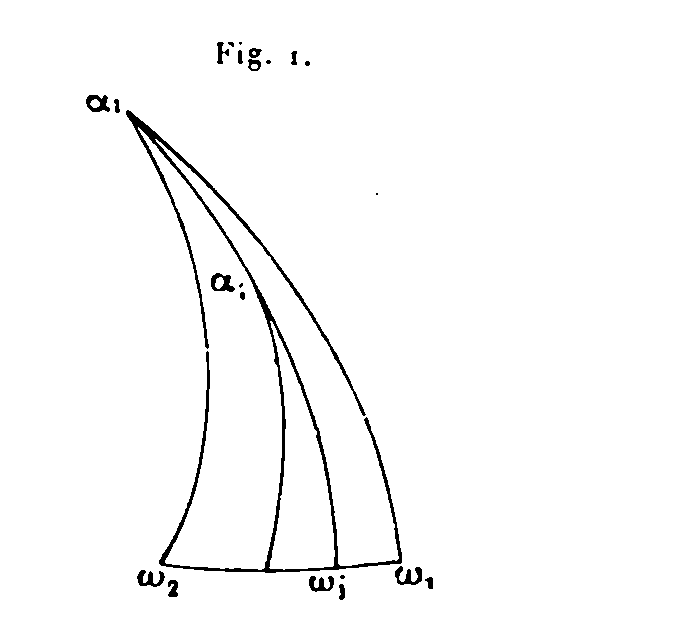
\includegraphics[width=0.43\textwidth]{fig1_scan.png}
\end{center}

Soient
\begin{align*}
&\beta_1 \text{ le point de la courbe C dont l’abscisse est } x_0;\\
&\alpha_1 \text{ le point correspondant de la caractéristique;}\\
&\alpha_1\omega_1 \text{ la tangente à la caractéristique en } \alpha_1;\\
&\omega_1 \text{ le point où } \alpha_1\omega_1 \text{ rencontre l’équateur;}\\
&\alpha_i \text{ un point quelconque de la caractéristique correspondant à un point } \beta_i \text{ situé à droite de } \beta_1;\\
&\alpha_i\omega_i \text{ la tangente en ce point;}\\
&\omega_i \text{ le point où cette tangente rencontre l’équateur.}
\end{align*}

Quand $\alpha_i$ s’avancera sur la caractéristique, $\omega_i$ se déplacera vers la droite, mais en restant toujours sur l’arc d’équateur $\omega_1\omega_2$\footnote{Actuellement, $\omega_2$ désigne l’une des extrémités d’un certain arc d’équateur $\omega_1\omega_2$, qui, en vertu de la troisième hypothèse, comprend tous les points $\omega_i$. (R. G.)}; la demi-caractéristique $\alpha_1\alpha_i$, qui ne peut franchir l’équateur, est convexe par hypothèse, et tout entière comprise dans le triangle sphérique $\alpha_1\omega_1\omega_2$, c’est-à-dire que sa longueur curviligne reste toujours plus petite que $\alpha_1\omega_1+\omega_1\omega_2$, c’est-à-dire qu’elle est finie, ce qui est absurde; la troisième hypothèse est donc inadmissible.

\emph{Quatrième hypothèse.} --- Quand $x$ varie depuis $x_0$ jusqu’à l’infini, l’ordonnée du point $\beta_i$, c’est-à-dire l’angle de direction de la tangente à la caractéristique, va toujours en croissant jusqu’à l’infini.

C’est-à-dire que l’angle de direction de la tangente à la caractéristique peut prendre toutes les valeurs
\[
y_0+n\pi,
\]
où $y_0$ est une constante donnée et $n$ un nombre positif entier quelconque. C’est dire que la tangente de l’angle de direction, c’est-à-dire le coefficient angulaire de la tangente à la caractéristique, est égale à
\[
\operatorname{tang} y_0
\]
pour un nombre infini de points $\beta_i$ différents.

Or le lieu des points où le coefficient angulaire de la tangente à la caractéristique est égal à $\operatorname{tang} y_0$ est une courbe algébrique qui ne peut, d’après l’hypothèse, rencontrer la demi-caractéristique qu’en un nombre fini de points $\alpha_i$. Il faut donc, encore ici, qu’à un point $\alpha_i$ correspondent une infinité de points $\beta_i$, c’est-à-dire que la caractéristique donnée soit un cycle.

En résumé, des quatre hypothèses que l’on peut faire, la première, la deuxième et la quatrième conduisent à ce résultat, que la caractéristique est un cycle; la troisième est inadmissible.

Le théorème est donc démontré.

\emph{Définition.} --- Nous appellerons \emph{polycycle} une courbe fermée comme le cycle, mais présentant des points doubles.

Exemple : intersection de la sphère avec un cylindre qui lui est tangent en un point.

\emph{Système topographique.} --- Si l’on trace sur la sphère un système de cycles et de polycycles, tel que par chacun des points de la sphère passe un cycle ou un polycycle, et un seul, excepté en quelques points singuliers par lesquels ne passe aucun cycle, nous dirons que ce système de cycles est un \emph{système topographique}, parce qu’il est analogue au système des courbes de niveau d’un terrain.

Les points doubles des polycycles sont alors analogues aux cols de ce terrain, les points singuliers par lesquels ne passe aucun cycle sont analogues aux \emph{fonds} et aux \emph{sommets} du terrain; de sorte que nous appellerons ces divers points : \emph{cols, fonds et sommets} du système.

Par exemple, le système des courbes
\[
f(x,y)=\operatorname{const.},
\]
où $f$ est un polynome entier en $x$ et en $y$, si ces courbes ne coupent pas l’équateur, est un système topographique. Les cols sont les points où l’on a à la fois
\[
\frac{df}{dx}=\frac{df}{dy}=0,
\qquad
\left(\frac{d^2f}{dx\,dy}\right)^2-\frac{d^2f}{dx^2}\frac{d^2f}{dy^2}>0;
\]
les sommets sont les points où l’on a
\[
\frac{df}{dx}=\frac{df}{dy}=0,
\qquad
\left(\frac{d^2f}{dx\,dy}\right)^2-\frac{d^2f}{dx^2}\frac{d^2f}{dy^2}<0,
\qquad
\frac{d^2f}{dx^2}<0;
\]
les fonds sont les points où l’on a
\[
\frac{df}{dx}=\frac{df}{dy}=0,
\qquad
\left(\frac{d^2f}{dx\,dy}\right)^2-\frac{d^2f}{dx^2}\frac{d^2f}{dy^2}<0,
\qquad
\frac{d^2f}{dx^2}>0.
\]

De même, si l’on a entre $z$, $x$ et $y$ une relation algébrique
\[
f(z,x,y)=0,
\]
telle que l’on n’ait jamais
\[
\frac{df}{dz}=0,
\]
et que $z$ ne puisse rester fini et réel quand $x$ et $y$ sont infinis et réels, le système des courbes
\[
z=\operatorname{const.}
\]
est un système topographique.

Par exemple, soit
\[
f(z,x,y)=(z-x)^2-2(x^2+y^2+1)=0;
\]
\[
\frac{df}{dz}
\]
ne peut être nul que si
\[
x^2+y^2+1=0,
\]
ce qui est impossible.

De plus, si l’on considère $z$ comme une constante, les termes du degré le plus élevé s’écrivent
\[
-(x^2+2y^2),
\]
c’est-à-dire que les courbes $z=\operatorname{const.}$ ne coupent pas l’équateur, c’est-à-dire que ces courbes forment un système topographique.

Le lieu des points où chacun des cycles d’un système topographique est tangent à une caractéristique s’appellera la \emph{courbe des contacts}.

Si le système topographique est algébrique, la courbe des contacts sera elle-même une courbe algébrique.

Si l’on considère un système topographique et l’un des polycycles du système correspondant à un des cols du système, une partie des fonds et des sommets est à l’extérieur du polycycle, une autre partie à l’intérieur, de sorte que chaque col \emph{distribue d’une certaine manière} les fonds et les sommets du système.

Deux systèmes topographiques sont \emph{analogues} lorsqu’ils ont mêmes cols, mêmes fonds, mêmes sommets et que les fonds et les sommets sont \emph{distribués de la même manière par les cols}.

\ornament

\setcounter{footnote}{0}

\begin{center}
{\bfseries CHAPITRE II.}\\[0.8em]
{\scshape Étude des caractéristiques dans le voisinage d’un point de la sphère.}
\end{center}

\shortline

Avant d’étudier les propriétés des caractéristiques dans toute l’étendue de la sphère, il faut rappeler les résultats déjà acquis relativement à l’étude de ces courbes dans une région limitée de la sphère. Les principaux théorèmes qui se rapportent à cette étude sont énoncés et démontrés dans divers Mémoires de Cauchy, intitulés \emph{Mémoires sur le calcul des limites}, et insérés aux tomes XIV, XV et XVI des \emph{Comptes rendus des séances de l’Académie des Sciences} et dans le célèbre Mémoire de MM. Briot et Bouquet, inséré dans le tome XXXVI du \emph{Journal de l’École Polytechnique}. Je me suis moi-même occupé de cette question dans une Note qui se trouve dans le XLV\textsuperscript{e} Cahier du \emph{Journal de l’École Polytechnique} et dans une Thèse pour le doctorat que j’ai soutenue devant la Faculté des Sciences de Paris\footnote{Voir ce Tome.}.

Supposons d’abord que le point autour duquel on veut étudier les caractéristiques soit
\[
x=\alpha,\qquad y=\beta.
\]
X et Y, qui sont des polynomes en $x$ et en $y$, peuvent être également considérés comme des polynomes en $x-\alpha$ et $y-\beta$.

De sorte que
\[
\begin{aligned}
X&=a_0+a_1(x-\alpha)+a_2(y-\beta)+\cdots,\\
Y&=b_0+b_1(x-\alpha)+b_2(y-\beta)+\cdots.
\end{aligned}
\]

\emph{Premier cas.} --- $a_0$ et $b_0$ ne sont pas nuls à la fois; supposons, par exemple,
\[
a_0\gtrless0;
\]
l’équation différentielle peut s’écrire
\[
\frac{dy}{dx}=\frac{Y}{X}=f(x,y),
\]
où $f$ est une série ordonnée suivant les puissances croissantes de $x-\alpha$ et $y-\beta$.

Donc, en vertu du théorème démontré par Cauchy (\emph{Comptes rendus}, t. XIV), $y$ peut s’exprimer par une série ordonnée suivant les puissances croissantes de $x-\alpha$ et se réduisant à $\beta$ pour $x=\alpha$.

Donc, par le point $(\alpha,\beta)$ passe une caractéristique et une seule.

\emph{Deuxième cas.} --- $a_0=b_0=0$.

Mais $a_1$, $a_2$, $b_1$ et $b_2$ ne sont pas nuls à la fois.

Le point $(\alpha,\beta)$ est alors un point singulier ordinaire. Commençons par rappeler un théorème relatif à ces points singuliers, théorème que j’ai démontré dans ma Thèse inaugurale.

\emph{Si l’équation}
\[
\begin{array}{r@{\quad}c}
(5)&(a_1-\lambda)(b_2-\lambda)-b_1a_2=0
\end{array}
\]
\emph{a deux racines différentes, $\lambda_1$ et $\lambda_2$;} 

\emph{Si le rapport de ces racines est positif ou imaginaire, l’intégrale générale de l’équation}
\[
\frac{dx}{X}=\frac{dy}{Y}
\]
\emph{est de la forme}
\[
z_1^{\lambda_1}z_2^{-\lambda_2}=\operatorname{const.},
\]
\emph{où $z_1$ et $z_2$ sont des séries ordonnées suivant les puissances croissantes de $x-\alpha$, $y-\beta$ et s’annulant pour}
\[
x=\alpha,\qquad y=\beta.
\]

Supposons que le point $(x,y)$ se rapproche indéfiniment du point $(\alpha,\beta)$, de telle façon que
\[
\lim\frac{y-\beta}{x-\alpha}=\mu;
\]
le coefficient angulaire de la tangente en ce point $(x,y)$ aura pour limite
\[
\frac{b_1+b_2\mu}{a_1+a_2\mu}.
\]

Donc la limite de la droite qui joint les points $(x,y)$ et $(\alpha,\beta)$ et la limite de la tangente à la caractéristique au point $(x,y)$ forment un faisceau homographique.

Les droites doubles de ce faisceau sont données par l’équation
\[
\mu(a_1+a_2\mu)=b_1+b_2\mu.
\]

Soient $\mu_1$ et $\mu_2$ les deux racines de cette équation; on calculera aisément $\lambda_1$ et $\lambda_2$ en fonctions rationnelles de $a_1$, $a_2$, $b_1$, $b_2$, $\mu_1$ et $\mu_2$.

Maintenant on peut diviser le deuxième cas en quatre cas subordonnés principaux.

\emph{Premier cas subordonné.} --- Les droites doubles du faisceau homographique sont réelles, et deux droites conjuguées quelconques du faisceau sont ou toutes deux dans l’angle aigu formé par les deux droites doubles, ou toutes deux dans l’angle obtus.

Dans ce cas, $\lambda_1$ et $\lambda_2$ sont réels et leur rapport est positif; le théorème que nous avons rappelé en commençant est donc applicable, et l’intégrale générale s’écrit
\[
z_1^{\lambda_1}z_2^{-\lambda_2}=\operatorname{const.},
\]
où $z_1$, $z_2$ sont des fonctions réelles de $x$ et de $y$ s’annulant pour
\[
x=\alpha,\qquad y=\beta,
\]
pendant que $\lambda_1$ et $\lambda_2$ sont deux nombres réels positifs.

Il s’ensuit que toutes les caractéristiques vont passer par le point singulier $(\alpha,\beta)$, pourvu qu’elles pénètrent dans une région de la sphère assez voisine de ce point pour que $z_1$ et $z_2$ soient convergents.

Un pareil point singulier s’appellera un \emph{nœud}.

Soit, par exemple, à étudier les caractéristiques qui satisfont à l’équation
\[
\frac{dx}{x}=\frac{dy}{2y}
\]
dans le voisinage du point
\[
x=y=0.
\]

L’équation générale de ces caractéristiques s’écrira
\[
y=kx^2,
\]
où $k$ est une constante. Dans le plan, cette équation représente une série de paraboles ayant même axe et ayant leur sommet à l’origine; sur la sphère, cette même équation représentera les intersections de la sphère avec les cônes, qui ont le centre de la sphère pour sommet et ces paraboles pour base.

Toutes ces intersections passent évidemment par le point
\[
x=y=0.
\]

\emph{Deuxième cas subordonné.} --- Les droites doubles du faisceau homographique sont réelles; mais deux droites conjuguées du faisceau sont situées de part et d’autre de ces deux droites doubles.

Dans ce cas, $\dfrac{\lambda_1}{\lambda_2}$ est réel et négatif, et le théorème dont nous avons parlé n’est plus applicable.

Mais MM. Briot et Bouquet ont fait voir, dans un Mémoire inséré au \emph{Journal de l’École Polytechnique}, XXXVI\textsuperscript{e} Cahier, qu’il passe par le point $(\alpha,\beta)$ deux caractéristiques et deux seulement.

Un pareil point singulier s’appellera un \emph{col}.

Soit, par exemple, à étudier dans le voisinage de l’origine des caractéristiques définies par l’équation
\[
\frac{dx}{x}=-\frac{dy}{y}.
\]

L’intégrale générale s’écrit
\[
xy=\operatorname{const.}
\]
et les seules caractéristiques qui passent par le point
\[
x=y=0
\]
sont les deux grands cercles
\[
x=0,\qquad y=0.
\]

\emph{Troisième cas subordonné.} --- Les droites doubles du faisceau homographique sont imaginaires, et ce faisceau ne se réduit pas à un système de droites en involution.

Dans ce cas, $\lambda_1$ et $\lambda_2$ sont deux imaginaires conjuguées et leur rapport est imaginaire. Le théorème général s’applique et l’intégrale générale s’écrit
\[
z_1^{\lambda_1}z_2^{-\lambda_2}=\operatorname{const.},
\]
où $z_1$ et $z_2$, $\lambda_1$ et $\lambda_2$ sont imaginaires conjuguées.

Soit
\[
\begin{aligned}
z_1&=\xi+i\eta,& \lambda_1&=\gamma+i\delta,\\
z_2&=\xi-i\eta,& \lambda_2&=-\gamma+i\delta.
\end{aligned}
\]

L’intégrale générale s’écrit alors
\[
(\xi^2+\eta^2)^\gamma\left(\frac{\xi+\eta i}{\xi-\eta i}\right)^{i\delta}=\operatorname{const.}
\]

Les courbes $\xi^2+\eta^2=\operatorname{const.}$ (où $\xi$ et $\eta$ sont des séries ordonnées suivant les puissances croissantes de $x-\alpha$ et $y-\beta$, et s’annulant pour $x=\alpha$, $y=\beta$) sont évidemment des cycles qui ne se coupent en aucun point et qui forment dans la région voisine du point $(\alpha,\beta)$ un système topographique dont le point $(\alpha,\beta)$ est un sommet.

Or, si l’on remarque que les équations
\[
\xi^2+\eta^2=A,
\qquad
\left(\frac{\xi+i\eta}{\xi-i\eta}\right)^i=B
\]
ne donnent pour $\xi$ et $\eta$, et par conséquent pour $x$ et $y$, qu’un seul système de valeurs réelles, on reconnaîtra que les caractéristiques ne coupent les cycles
\[
\xi^2+\eta^2=A
\]
qu’en un seul point et que, par conséquent, ces caractéristiques ne sont autre chose que des spirales; un point qui parcourt ces spirales dans un certain sens va en se rapprochant indéfiniment de l’origine.

Un pareil point singulier s’appellera un \emph{foyer}.

Soit, par exemple, l’équation
\[
\frac{dx}{x-y}=\frac{dy}{x+y},
\]
dont l’intégrale générale est
\[
(x^2+y^2)\left(\frac{x+iy}{x-iy}\right)^i=\operatorname{const.}
\]

Si l’on passe aux coordonnées polaires, cette intégrale devient
\[
\rho^2e^{-2\omega}=\operatorname{const.},
\]
ce qui nous donne, dans le plan, une spirale logarithmique, et, par conséquent, sur la sphère, une spirale sphérique.

\emph{Quatrième cas subordonné.} --- Les droites doubles du faisceau homographique sont imaginaires et ce faisceau se réduit à un système de droites en involution.

Dans ce cas, $\lambda_1$ et $\lambda_2$ sont imaginaires conjuguées, mais leur rapport est égal à $-1$. Le théorème que nous avons rappelé au début n’est donc pas applicable en général.

Ce quatrième cas est plus particulier que les précédents et il ne se présentera pas si X et Y sont les polynomes les plus généraux de leur degré. Bornons-nous donc à quelques remarques.

D’abord, il est impossible qu’une branche de caractéristique vienne passer par le point $\alpha$, $\beta$, puisque sa tangente devrait être précisément l’une des droites doubles de l’involution qui sont imaginaires.

Mais, d’après ce qu’on verra plus loin, toute caractéristique est un cycle ou une spirale; donc, ou bien les caractéristiques seront des spirales, et un point qui les parcourrait tournerait autour du point $(\alpha,\beta)$ en s’en rapprochant indéfiniment : le point $(\alpha,\beta)$ serait alors encore un \emph{foyer}; ou bien les caractéristiques forment un système topographique dont $(\alpha,\beta)$ est un sommet, et alors le point $(\alpha,\beta)$ est un \emph{centre}.

C’est ce qui arrive quand le théorème que nous énoncions au début est applicable, malgré la valeur négative de $\dfrac{\lambda_1}{\lambda_2}$.

En effet, dans ce cas, l’intégrale s’écrit
\[
z_1z_2=A,
\]
où
\[
z_1=\xi+i\eta,
\qquad
z_2=\xi-i\eta;
\]
c’est-à-dire
\[
\xi^2+\eta^2=A;
\]
et les caractéristiques forment évidemment, dans ce cas, un système topographique de cycles.

Par exemple, l’équation
\[
\frac{dx}{y}=\frac{dy}{-x}
\]
a pour intégrale générale
\[
x^2+y^2=A.
\]

\emph{Cas particuliers laissés de côté.} --- Dans ce qui précède, on a laissé de côté les cas particuliers où
\[
\lambda_1=\lambda_2,
\qquad
\lambda_1=0,
\]
cas qui ne se présenteront pas si X et Y sont les polynomes les plus généraux de leur degré.

Or, pour que
\[
\lambda_1=\lambda_2,
\]
il faut et il suffit que
\[
(a_1+b_2)^2-b_1a_2+a_1b_2=0.
\]

Dans ce cas, MM. Briot et Bouquet ont fait voir qu’une infinité de caractéristiques passent par le point $(\alpha,\beta)$, c’est-à-dire qu’on a encore affaire à un \emph{nœud}.

Les cinq cas précédents comprennent tous les points singuliers $\alpha$, $\beta$, tels que les deux courbes
\[
X=0,\qquad Y=0
\]
s’y coupent en un seul point et non en plusieurs points confondus. Ces points singuliers s’appelleront \emph{points singuliers de première espèce}, et l’on a vu qu’il y avait quatre sortes de pareils points : les nœuds, les cols, les foyers et les centres.

Reste à examiner les cas où
\[
\lambda_1=0
\]
et ceux où
\[
a_1=a_2=0
\]
ou
\[
b_1=b_2=0.
\]

Ces cas se présentent quand les courbes $X=Y=0$ se coupent en plusieurs points confondus au point $(\alpha,\beta)$.

En effet, dire que
\[
a_1=a_2=0,
\]
c’est dire que $X=0$ offre un point multiple en $(\alpha,\beta)$.

Dire que
\[
b_1=b_2=0,
\]
c’est dire que $Y=0$ offre un point multiple en $(\alpha,\beta)$.

Dire que
\[
\lambda_1=0,
\]
c’est dire que
\[
\frac{a_1}{a_2}=\frac{b_1}{b_2},
\]
c’est-à-dire que les courbes $X=0$, $Y=0$ sont tangentes au point $(\alpha,\beta)$.

De pareils points singuliers s’appelleront \emph{points singuliers de seconde espèce}, et il est évident, d’après ce qui précède, qu’ils pourront toujours être considérés comme la limite d’un système de plusieurs points singuliers de première espèce confondus ensemble.

Les particularités que peuvent présenter de pareils points sont trop nombreuses et trop diverses pour que nous les étudiions en détail. Remarquons que de pareils points ne peuvent exister si X et Y sont les polynomes les plus généraux de leur degré.

\emph{Points situés sur l’équateur.} --- Dans ce qui précède, on a supposé implicitement que $\alpha$ et $\beta$ restent finis, c’est-à-dire que le point $(\alpha,\beta)$ n’est pas sur l’équateur.

Mais le cas où $\alpha$, $\beta$ est sur l’équateur peut se ramener aisément aux cas déjà étudiés.

Considérons d’abord un point de l’équateur non situé sur le grand cercle
\[
x=0;
\]
nous poserons
\[
x=\frac1z,
\qquad
y=\frac{t}{z}.
\]

Si l’on considère ensuite $z$ et $t$ comme les coordonnées d’un point dans un plan, ce point ne sera autre chose que la projection gnomonique du point $(x,y)$ de la sphère sur un plan parallèle au plan du grand cercle
\[
x=0.
\]

Pour le point $(\alpha,\beta)$ de la sphère, ces coordonnées $z$ et $t$ seront finies, c’est-à-dire qu’on sera ramené aux cas étudiés dans le commencement de ce Chapitre.

Si l’on voulait étudier les caractéristiques dans le voisinage de l’intersection de l’équateur et du grand cercle
\[
x=0,
\]
on poserait
\[
x=\frac{t}{z},
\qquad
y=\frac1z,
\]
et l’on raisonnerait de la même manière.

\ornament


\ornament
\begin{center}
{\Large CHAPITRE III.}\\[0.4em]
{\small DISTRIBUTION DES POINTS SINGULIERS.}
\end{center}
\shortline

\emph{Théorème II.} --- \emph{Tout système de caractéristiques admet des points singuliers.}

\emph{Première hypothèse.} --- Les courbes
\[
X=0,\qquad Y=0
\]
se coupent en des points non situés sur l’équateur.

Dans ce cas, ces points d’intersection sont évidemment des points singuliers.

\emph{Deuxième hypothèse.} --- Les courbes
\[
X=0,\qquad Y=0
\]
se coupent en un point situé sur l’équateur.

Supposons que ce point ne soit pas sur le grand cercle
\[
x=0;
\]
nous poserons
\[
x=\frac1z,\qquad y=\frac{t}{z},
\]
et, si $m$ est le degré de celui des deux polynomes X et Y dont le degré est le plus élevé, nous poserons
\[
z^mX=X_1,\qquad z^mY=Y_1.
\]
L’équation différentielle devient alors
\[
\frac{dz}{zX_1}=\frac{dt}{Y_1-tX_1};
\]
pour $t=\alpha$, $z=0$, on a, par hypothèse,
\[
Y_1=X_1=0,
\]
et par conséquent
\[
zX_1=0,\qquad Y_1-tX_1=0,
\]
c’est-à-dire que le point
\[
t=\alpha,\qquad z=0
\]
est un point singulier de l’équation proposée.

\emph{Troisième hypothèse.} --- Les courbes $X=0$, $Y=0$ ne se coupent en aucun point. Le degré de X est plus grand que celui de Y. Dans ce cas, l’un au moins des deux polynomes X et Y est de degré pair. De plus $Y_1$ est divisible par $z$, de sorte que
\[
Y_1=zY_2.
\]
Or il est clair que pour
\[
z=t=0,
\]
on a
\[
zX_1=zY_2-tX_1=0,
\]
et que par conséquent le point
\[
z=t=0
\]
est un point singulier.

\emph{Quatrième hypothèse.} --- Les courbes $X=0$, $Y=0$ ne se coupent en aucun point. Le degré de X est inférieur à celui de Y. Dans ce cas on poserait
\[
x=\frac{t}{z},\qquad y=\frac1z,
\]
et, en raisonnant comme dans le cas précédent, on ferait voir que
\[
z=t=0
\]
est un point singulier.

\emph{Cinquième hypothèse.} --- Les courbes $X=0$, $Y=0$ ne se coupent en aucun point. Le degré de X et de Y est le même.

Si, de plus, $X_2$ et $Y_2$ sont les termes du degré le plus élevé de X et Y, on n’a pas identiquement
\[
xY_2-yX_2=0.
\]
Dans ce cas, le degré de X et de Y étant $m$, et nécessairement pair, la fonction $xY_2-yX_2$ est homogène en $x$ et $y$ et de degré $m+1$, et par conséquent de degré impair.

Elle s’annule donc, soit pour $x=0$, soit pour une certaine valeur finie de $\dfrac yx$.

Si elle s’annule pour une certaine valeur $\alpha$ de $\dfrac yx$, on aura à la fois pour
\[
t=\alpha,\qquad z=0,
\]
\[
zX_1=Y_1-tX_1=0
\]
quand on aura posé
\[
x=\frac1z,\qquad y=\frac{t}{z},
\]
c’est-à-dire que le point
\[
t=\alpha,\qquad z=0
\]
sera un point singulier.

Si la fonction $xY_2-yX_2$ s’annule pour $x=0$, on posera
\[
x=\frac{t}{z},\qquad y=\frac1z,
\]
et l’on verra, comme précédemment, que le point
\[
t=z=0
\]
est un point singulier.

\emph{Sixième hypothèse.} --- Les courbes X et Y ne se coupent en aucun point. Le degré de X est le même que celui de Y; si, de plus, $X_2$ et $Y_2$ sont les termes du degré le plus élevé de X et de Y, on a identiquement
\[
xY_2-yX_2=0.
\]
Cette hypothèse est inadmissible.

En effet, si l’on a identiquement
\[
xY_2=yX_2,
\]
$X_2$ est divisible par $x$ et égal à $xX_3$, $Y_2$ est divisible par $y$ et égal à $yY_3$, de sorte que l’on a identiquement
\[
xyY_3=yxX_3
\]
ou
\[
Y_3=X_3.
\]
Maintenant $Y_3=X_3$ est une fonction homogène de degré impair en $x$ et en $y$; donc elle s’annule soit pour $x=0$, soit pour une certaine valeur réelle $\alpha$ de $\dfrac yx$.

Donc, soit pour $x=0$, soit pour $\dfrac yx=\alpha$, on aurait forcément
\[
X_2=Y_2=0,
\]
c’est-à-dire que les courbes $X=0$, $Y=0$ se couperaient en un point de l’équateur, ce qui est contraire à l’hypothèse.

En résumé, des six hypothèses que l’on peut faire, la sixième est inadmissible; si l’une des cinq autres est réalisée, l’équation différentielle admet des points singuliers, soit sur l’équateur, soit hors de l’équateur.

\emph{Cas général.} --- On peut, sans nuire à la généralité, supposer :

1° Que les polynomes X et Y sont de même degré;

2° Que si $X_2$ et $Y_2$ sont les termes du degré le plus élevé de X et de Y, on n’a pas identiquement
\[
xY_2-yX_2=0;
\]
3° Que les courbes $X=Y=0$ ne se coupent nulle part en plusieurs points confondus et ne se coupent pas sur l’équateur;

4° Que l’équation
\[
xY_2-yX_2=0
\]
n’a pas de racines multiples.

Dans ce cas, \emph{l’équateur est toujours une caractéristique}, et tous les points singuliers sont de première espèce. De plus, on peut, sans nuire à la généralité, supposer que tous les points singuliers sont des \emph{nœuds}, des \emph{cols} et des \emph{foyers}.

\emph{Le nombre des points singuliers est évidemment pair}, puisque tout est symétrique par rapport au centre de la sphère.

Le nombre minimum des points singuliers est donc égal à $2$, et ce cas peut se présenter de deux manières :

1° Les courbes
\[
X=0,\qquad Y=0
\]
ne se coupent en aucun point; mais l’équation homogène
\[
xY_2-yX_2=0
\]
admet une solution réelle et une seule.

On a alors sur l’équateur deux points singuliers diamétralement opposés. Je dis que ces points singuliers sont toujours des nœuds. Pour le démontrer, il faut étudier les propriétés générales des points singuliers situés sur l’équateur.

Supposons que pour
\[
t=\alpha,\qquad z=0,
\]
on ait
\[
zX_1=Y_1-tX_1=0
\]
et
\[
X_1\gtrless0,\qquad Y_1\gtrless0.
\]
Posons
\[
t=u+\alpha,
\]
et soit
\[
\begin{aligned}
X_1&=z\xi_1+\lambda_0+\lambda_1u+\lambda_2u^2+\cdots+\lambda_mu^m,\\
Y_1&=z\eta_1+\mu_0+\mu_1u+\mu_2u^2+\cdots+\mu_mu^m,
\end{aligned}
\]
où $\xi_1$ et $\eta_1$ sont des polynomes entiers en $z$ et en $u$, et où les $\lambda$ et les $\mu$ sont des constantes. Il vient, en posant
\[
\begin{aligned}
\lambda_2u^2+\cdots+\lambda_mu^m&=\xi_2u^2,\\
\mu_2u^2+\cdots+\mu_mu^m&=\eta_2u^2,\\
X_1&=u^2\xi_2+z\xi_1+\lambda_0+\lambda_1u,\\
Y_1&=u^2\eta_2+z\eta_1+\mu_0+\mu_1u;
\end{aligned}
\]
d’où l’on tire
\[
Y_1-tX_1=z\theta_1+u^2\theta_2+(\mu_0-\lambda_0\alpha)+(\mu_1-\lambda_1\alpha-\lambda_0)u,
\]
où $\theta_1$ et $\theta_2$ sont des polynomes entiers en $z$ et $u$. L’équation différentielle s’écrit alors, en remarquant que l’on doit avoir $\mu_0=\lambda_0\alpha$,
\[
\frac{dz}{z(\lambda_0+\lambda_1u+z\xi_1+u^2\xi_2)}=
\frac{du}{(\mu_1-\lambda_1\alpha-\lambda_0)u+z\theta_1+u^2\theta_2}.\tag{1}
\]
Les racines de l’équation (5) sont alors
\[
-\lambda_0\quad\text{et}\quad \mu_1-\lambda_1\alpha-\lambda_0.
\]
Ces deux racines sont réelles.

Donc \emph{tout point singulier situé sur l’équateur est un nœud ou un col}. (C’est ce qu’on devait prévoir, l’équateur étant une caractéristique.)

Pour qu’il soit un nœud, il faut et il suffit que
\[
\lambda_0^2+\lambda_0\lambda_1\alpha-\lambda_0\mu_1>0.
\]
Or le premier membre de cette inégalité est précisément la valeur que prend, pour
\[
y=x\alpha,
\]
l’expression
\[
-\frac1{x^{2m}}\frac{d}{dy}(xY_2X_2-yX_2^2).
\]
Nous n’en changerons pas le signe en écrivant\footnote{Dans cette phrase, une erreur de rédaction a été corrigée. (R. G.).}
\[
-\frac{d}{dy}\left(\frac{Y_2}{X_2}-\frac yx\right),
\]
c’est-à-dire que le point singulier
\[
\frac yx=\alpha
\]
sera un col si, quand $\dfrac yx$ passe de $\alpha-\varepsilon$ à $\alpha+\varepsilon$, l’expression $\dfrac{Y_2}{X_2}-\dfrac yx$ passe du négatif au positif, et qu’il sera un nœud si, quand $\dfrac yx$ passe de $\alpha-\varepsilon$ à $\alpha+\varepsilon$, l’expression $\dfrac{Y_2}{X_2}-\dfrac yx$ passe du positif au négatif.

Cela posé, nous allons introduire une considération nouvelle qui nous rendra les plus grands services. Soit un cycle situé tout entier dans un hémisphère. Ce cycle divise la sphère en deux régions, dont l’une, située tout entière dans l’un des hémisphères, s’appellera \emph{l’intérieur du cycle}.

Si le cycle est tout entier dans le premier hémisphère, nous dirons qu’un point mobile décrit le cycle dans le sens positif s’il a constamment l’intérieur du cycle \emph{à sa gauche}; si au contraire, le cycle était dans le second hémisphère, un point décrirait le cycle dans le sens positif s’il en avait constamment l’intérieur \emph{à sa droite}.

Supposons qu’un point mobile décrive le cycle dans le sens positif et considérons les variations de l’expression $\dfrac YX$. Soit $h$ le nombre de fois que cette expression saute de $-\infty$ à $+\infty$; soit $k$ le nombre de fois que cette expression saute de $+\infty$ à $-\infty$. Soit
\[
i=\frac{h-k}{2};
\]
le nombre $i$ s’appellera \emph{l’indice du cycle}.

Si l’on joint deux points A et C d’un cycle ABCDA par un arc AMC situé
\begin{center}
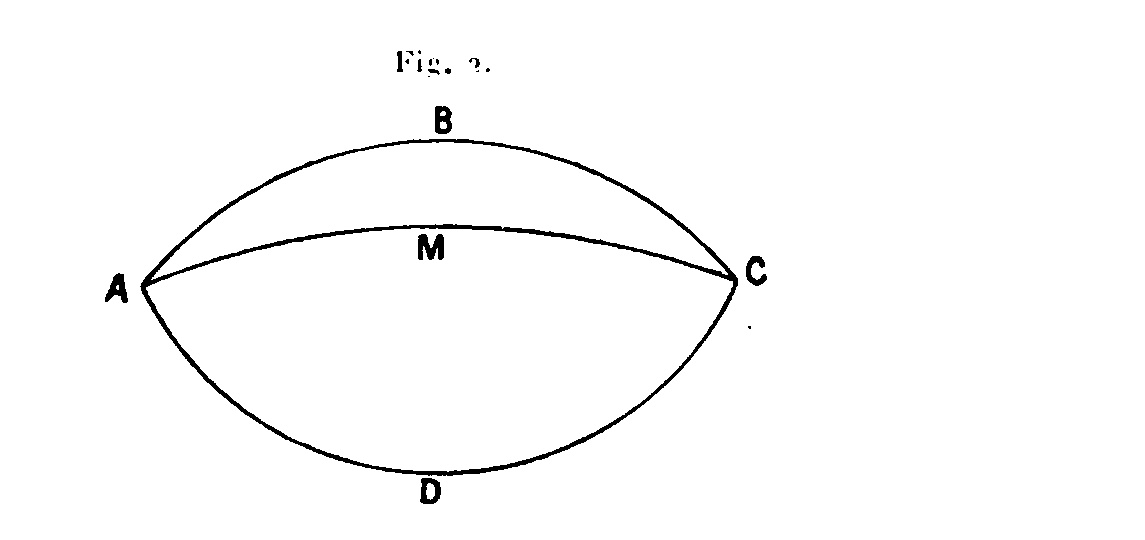
\includegraphics[width=0.48\textwidth]{fig2_scan.jpg}
\end{center}
tout entier à l’intérieur du cycle, le cycle ABCDA se trouve décomposé en deux cycles ABCMA, AMCDA, et l’on a évidemment
\[
\operatorname{ind.}ABCDA=\operatorname{ind.}ABCMA+\operatorname{ind.}AMCDA,
\]
de sorte qu’on peut ramener le calcul de l’indice d’un cycle quelconque au calcul de l’indice des différents cycles infiniment petits qui le composent.

\emph{Théorème III.} --- \emph{Un cycle infiniment petit qui ne contient à son intérieur aucun point singulier a pour indice $0$.}

En effet, si ce cycle n’est pas coupé par la courbe $X=0$,
\[
h=0,\qquad k=0,\qquad i=\frac{h-k}{2}=0.
\]
Si le cycle est coupé par la courbe $X=0$, il n’est pas coupé par la courbe $Y=0$; Y est toujours de même signe et X passe une fois du positif au négatif, une fois du négatif au positif; d’où
\[
h=1,\qquad k=1,\qquad i=\frac{h-k}{2}=0.
\]
De même, si la courbe $X=0$ présentait à l’intérieur du cycle un point multiple d’ordre $m$, on aurait
\[
h=m,\qquad k=m,\qquad i=\frac{h-k}{2}=0.
\]

\emph{Théorème IV.} --- \emph{Si un cycle infiniment petit contient à son intérieur un point singulier, son indice est égal à $\pm1$.}

Il est égal à $+1$ si le point singulier est un col; à $-1$ si le point singulier est un nœud ou un foyer.

En effet, posons
\[
y-\beta=\rho\sin\omega,\qquad x-\alpha=\rho\cos\omega,
\]
et supposons que l’on considère le cycle
\[
(y-\beta)^2+(x-\alpha)^2=\rho^2,
\]
$\rho$ étant une constante infiniment petite.

Pour décrire ce cycle dans le sens positif, il faut faire varier $\omega$ depuis $0$ jusqu’à $2\pi$.

Or on a, en négligeant les infiniment petits et reprenant les notations du Chapitre précédent,
\[
\frac YX=\frac{b_1+b_2\operatorname{tang}\omega}{a_1+a_2\operatorname{tang}\omega}.
\]
X s’annule deux fois, car, quand $\omega$ varie depuis $0$ jusqu’à $2\pi$,
\[
a_1+a_2\operatorname{tang}\omega
\]
s’annule deux fois pour deux valeurs de $\omega$ que nous appellerons $\omega_0$ et $\omega_0+\pi$.

Pour $\omega=\omega_0-\varepsilon$, où $\varepsilon$ est infiniment petit, on a
\[
\operatorname{tang}\omega=\operatorname{tang}\omega_0-\zeta,
\]
où $\zeta$ est positif et infiniment petit. On a donc
\[
\frac YX=\frac{b_1+b_2\operatorname{tang}\omega_0-b_2\zeta}{a_1+a_2\operatorname{tang}\omega_0-a_2\zeta}.
\]
Remarquons que $\operatorname{tang}\omega_0=-\dfrac{a_1}{a_2}$; il viendra, en négligeant $b_2\zeta$ devant $b_1+b_2\operatorname{tang}\omega_0$,
\[
\frac YX=\frac{a_1b_2-a_2b_1}{a_2^2}\,\frac1\zeta.
\]
Donc, si $a_1b_2-a_2b_1<0$, $\dfrac YX$ pour $\omega=\omega_0$ et pour $\omega=\omega_0+
\pi$ saute de $-\infty$ à $+\infty$, on a
\[
h=2,\qquad k=0,\qquad i=\frac{h-k}{2}=1.
\]
Si, au contraire, $a_1b_2-a_2b_1>0$, $\dfrac YX$ pour $\omega=\omega_0$ et pour $\omega=\omega_0+
\pi$ saute de $+\infty$ à $-\infty$, on a
\[
h=0,\qquad k=2,\qquad i=\frac{h-k}{2}=-1.
\]
Maintenant, quelle est la condition pour que
\[
a_1b_2-a_2b_1>0?
\]
Reprenons l’équation (5) qui s’écrit
\[
(a_1-\lambda)(b_2-\lambda)-a_2b_1=0.
\]
Il est évident qu’on aura
\[
a_1b_2-a_2b_1>0,
\]
si les deux racines de l’équation sont imaginaires ou de même signe, c’est-à-dire si le point singulier est un nœud ou un foyer. On aura au contraire
\[
a_1b_2-a_2b_1<0,
\]
si les deux racines sont réelles et de signe contraire, c’est-à-dire si le point singulier est un col.

Le théorème est donc démontré.

\emph{Problème I.} --- \emph{Calculer l’indice d’un cycle situé tout entier dans l’un des hémisphères.}

Soient N le nombre des nœuds, F le nombre des foyers, C le nombre des cols contenus à l’intérieur du cycle.

Si l’on décompose le cycle donné en une infinité de cycles infiniment petits $\gamma$,
\[
\begin{array}{rcl}
\text{Un nombre infini des cycles }\gamma\text{ auront pour indice} & 0,\\
N+F\text{ des cycles }\gamma & -1,\\
C\text{ des cycles }\gamma & +1.
\end{array}
\]
L’indice du cycle donné sera donc
\[
-(N+F-C).
\]

\emph{Problème II.} --- \emph{Calculer l’indice de l’équateur.}

Soient $2N'$ le nombre des nœuds, $2C'$ le nombre des cols situés sur l’équateur.

Soit $t=\dfrac yx=\operatorname{tang}\omega$.

Faisons varier $\omega$ depuis $-\dfrac\pi2$ jusqu’à $+\dfrac\pi2$, c’est-à-dire $\operatorname{tang}\omega$ depuis $-\infty$ jusqu’à $+\infty$. Tout étant symétrique par rapport au centre de la sphère,
\[
\frac YX=\frac{Y_2}{X_2}
\]
prend pour $\omega+\pi$ la même valeur que pour $\omega$; quand on ferait varier $\omega$ depuis $+\dfrac\pi2$ jusqu’à $+\dfrac{3\pi}{2}$, $\dfrac YX$ repasserait par les mêmes valeurs que quand $\omega$ variait de $-\dfrac\pi2$ à $+\dfrac\pi2$.

Donc, $\omega$ variant de $-\dfrac\pi2$ à $+\dfrac\pi2$, $\dfrac YX$ sautera $\dfrac h2$ fois de $-\infty$ à $+\infty$, et $\dfrac k2$ fois de $+\infty$ à $-\infty$.

Ceci posé, si l’on considère l’expression
\[
H=\frac{Y_2}{X_2}-\frac yx=\frac YX-\operatorname{tang}\omega,
\]
pour $\omega=-\dfrac\pi2$, on a
\[
H=+\infty;
\]
pour $\omega=+\dfrac\pi2$, on a
\[
H=-\infty.
\]
Soient $\lambda$ le nombre de fois que H passe du négatif au positif, $\mu$ le nombre de fois que H passe du positif au négatif; on aura évidemment
\[
\mu-\lambda=1.
\]
Or H peut passer du négatif au positif, soit par 0, ce qui correspond à un col, soit par $\infty$, ce qui correspond à l’une des valeurs des $\dfrac h2$ valeurs de $\omega$, pour lesquelles $\dfrac YX$ saute de $-\infty$ à $+\infty$.

On a donc
\[
\lambda=C'+\frac h2.
\]
De même
\[
\mu=N'+\frac k2;
\]
d’où
\[
N'-C'=1+\frac{h-k}{2}=1+i,
\]
d’où
\[
i=N'-C'-1.
\]

\emph{Scolie.} --- Si le nombre des nœuds situés hors de l’équateur est $2N$, celui des foyers situés hors de l’équateur $2F$, celui des cols situés hors de l’équateur $2C$, celui des nœuds situés sur l’équateur $2N'$, celui des cols situés sur l’équateur $2C'$, on a la relation
\[
N'+N+F=C+C'+1.
\]
En effet, pour obtenir ce résultat, il suffit d’égaler les deux valeurs de l’indice de l’équateur obtenues dans les deux problèmes précédents.

\emph{Corollaire I.} --- Le nombre total des nœuds et des foyers est égal au nombre total des cols plus $2$.

\emph{Corollaire II.} --- Le nombre total des points singuliers est un multiple de $4$ plus $2$.

\emph{Corollaire III.} --- Si le nombre des points singuliers se réduit à $2$, ces points sont des nœuds et des foyers; ils sont toujours des nœuds s’ils sont sur l’équateur.

La courbe $X=0$ et la courbe $Y=0$ se composent d’un certain nombre de cycles. Considérons deux quelconques de ces cycles : ils se couperont en un nombre pair de points.

Soient $\alpha_0$, $\alpha_1$, \ldots, $\alpha_{2n}$ les $2n$ points d’intersection de ces deux cycles rangés d’après l’ordre où on les rencontre en parcourant l’un des deux cycles, le cycle $X=0$, par exemple, dans le sens positif.

\emph{Théorème V.} --- \emph{Supposons que deux points consécutifs $\alpha_k$ et $\alpha_{k+1}$ soient situés dans le même hémisphère : je dis que si $\alpha_k$ est un nœud ou un foyer, $\alpha_{k+1}$ est un col, ou réciproquement.}

Pour cela il suffit de faire voir que tout cycle qui enveloppe $\alpha_k$ et $\alpha_{k+1}$ a pour indice $0$.

En effet, soit (fig. 3) AB l’arc du cycle $X=0$, sur lequel se trouvent les points $\alpha_k$ et $\alpha_{k+1}$; soient CD et EF les arcs du cycle $Y=0$ qui viennent couper AB respectivement en $\alpha_k$ et $\alpha_{k+1}$.
\begin{center}
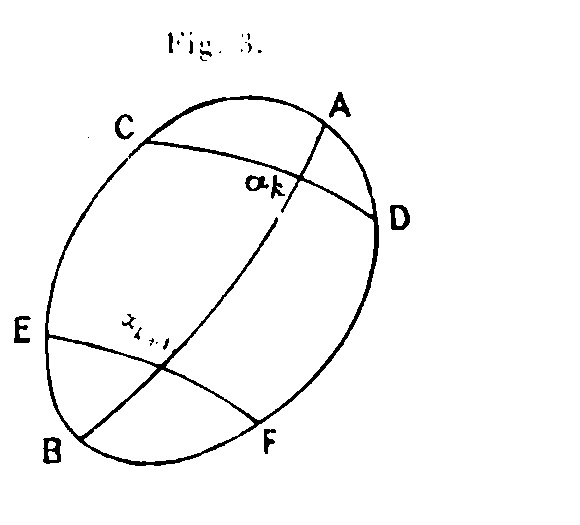
\includegraphics[width=0.30\textwidth]{fig3_scan.jpg}
\end{center}
Il est évident que, pour le cycle ADFBECA,
\[
h=1,\qquad k=1,\qquad i=\frac{h-k}{2}=0.
\]
Supposons, au contraire, que les points $\alpha_k$ et $\alpha_{k+1}$ soient dans deux hémisphères différents :
\begin{center}
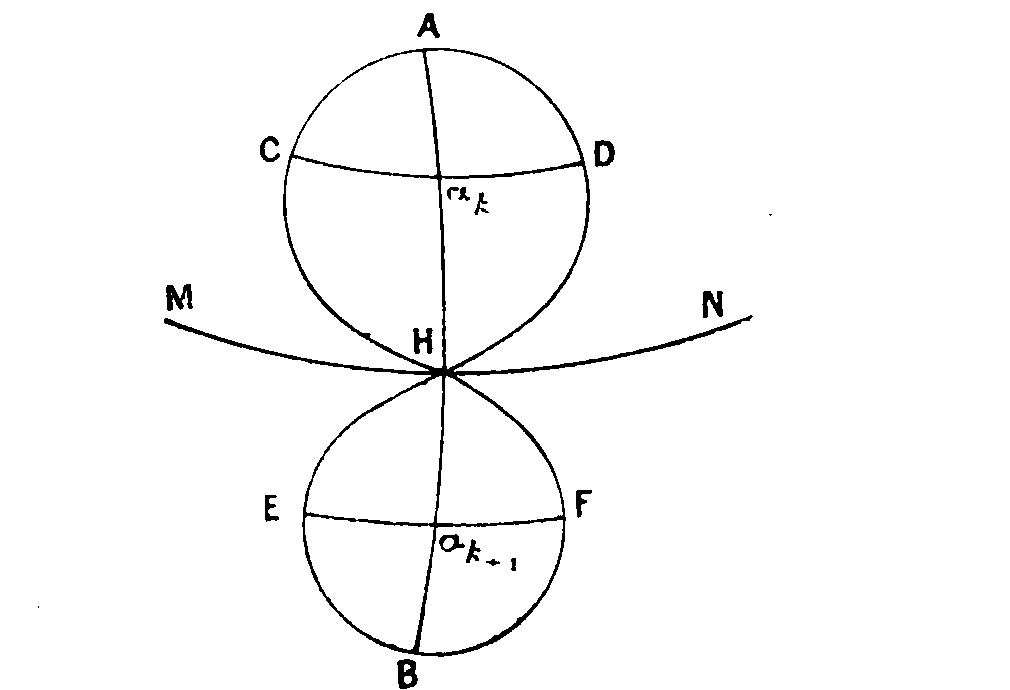
\includegraphics[width=0.38\textwidth]{fig4_scan.jpg}
\end{center}
Je dis que si $\alpha_k$ est un col, $\alpha_{k+1}$ est un col, et que si $\alpha_k$ est un nœud ou un foyer, $\alpha_{k+1}$ est un nœud ou un foyer.

En effet, supposons que AB vienne couper l’équateur MN en H (fig. 4). Considérons le cycle ACHFBEHDA. Ce cycle est parcouru \emph{dans les deux hémisphères} dans le sens positif.

Supposons qu’en franchissant le point A, $\dfrac YX$ saute de $-\infty$ à $+\infty$; il en sera de même quand on franchira le point H ou le point B, c’est-à-dire que si
\[
\operatorname{ind.}ACHD=1,\qquad \operatorname{ind.}ACHFBEHDA=2.
\]
De même, si
\[
\operatorname{ind.}ACHD=-1,\qquad \operatorname{ind.}ACHFBEHDA=-2,
\]
c’est-à-dire que, dans tous les cas,
\[
\operatorname{ind.}ACHDA=\operatorname{ind.}HFBEH.
\]
C. Q. F. D.

\emph{Deuxième cas.} --- Dans tout ce qui précède, nous avons supposé que $X_2$ et $Y_2$ étaient de même degré, sans que
\[
xY_2-yX_2
\]
soit identiquement nul.

Nous n’avons pas examiné ce qui se passerait si nous avions identiquement
\[
xY_2-yX_2=0.
\]
À un certain point de vue, le cas que nous avons étudié est plus général que celui que nous avons laissé de côté.

À un autre point de vue, c’est le contraire; car deux polynomes X et Y quelconques peuvent être considérés comme des cas particuliers des polynomes
\[
X+\lambda xZ,
\qquad
Y+\lambda yZ,
\]
où $\lambda$ est une constante et Z un polynome de même degré que X et Y.

Nous allons donc supposer que l’on a identiquement
\[
X_2=xZ,
\qquad
Y_2=yZ,
\]
où Z est une fonction homogène en $x$ et $y$.

Dans ce cas, \emph{l’équateur n’est plus une caractéristique}, et par conséquent les points singuliers de l’équateur peuvent être tout aussi bien des nœuds, des foyers et des cols.

La règle qui permettait, dans le cas précédent, de trouver l’indice de l’équateur se trouve en défaut; d’ailleurs, si l’équateur contient des points singuliers, les courbes
\[
X=0,
\qquad
Y=0
\]
se coupent sur ce grand cercle, qui n’a par conséquent plus, à proprement parler, d’indice.

Supposons donc que l’équateur ne contienne pas de point singulier, et cherchons quel est l’indice de ce grand cercle.

Nous trouverons que l’on a le long de l’équateur
\[
\frac YX=\frac yx,
\]
c’est-à-dire que l’indice de l’équateur sera égal à $-1$, et si l’on remarque qu’il est déjà égal à
\[
-(N+F-C),
\]
$2N$, $2F$, $2C$ étant le nombre des nœuds, des foyers et des cols, on reconnaîtra que l’on a
\[
F+N=C+1,
\]
c’est-à-dire que le théorème que l’on avait démontré dans le cas précédent est encore vrai.

Supposons maintenant que l’équation contienne des points singuliers, à savoir $2N'$ nœuds, $2F'$ foyers et $2C'$ cols, et voyons comment on pourra tourner la difficulté.

Soit $\alpha x+\beta y+\gamma=0$ un grand cercle qui ne passe par aucun point singulier.

Posons
\[
x'=\frac{x}{\alpha x+\beta y+\gamma},
\qquad
 y'=\frac{y}{\alpha x+\beta y+\gamma};
\]
l’équation différentielle devient
\[
\frac{dx'}{X'}=\frac{dy'}{Y'},
\]
où $X'$ et $Y'$ sont des polynomes entiers en $x'$ et $y'$.

On aura pu choisir le cercle $\alpha x+\beta y+\gamma=0$, de telle façon que :

1° Aucune réduction ne s’opérant, $X'$ et $Y'$ soient de même degré;

2° Que le grand cercle $\alpha x+\beta y+\gamma=0$ ne soit pas une caractéristique, c’est-à-dire que les termes du degré le plus élevé de $y'X'-x'Y'$ se réduisent.

Si $a$, $b$ est un point singulier de l’équation
\[
\frac{dx}{X}=\frac{dy}{Y},
\]
\[
a'=\frac{a}{\alpha a+\beta b+\gamma},
\qquad
b'=\frac{b}{\alpha a+\beta b+\gamma},
\]
sera aussi un point singulier de l’équation
\[
\frac{dx'}{X'}=\frac{dy'}{Y'}.
\]
Si $a$, $b$ est un nœud, un col ou un foyer, $a'$, $b'$ sera un nœud, un col ou un foyer, de sorte que les nombres des nœuds, des cols et des foyers sont $2(N+N')$, $2(C+C')$, $2(F+F')$ et que, se trouvant ramené au cas où l’équateur ne contenait pas de point singulier, on peut écrire
\[
N+N'+F+F'=C+C'+1.
\]

\ornament



\ornament
\begin{center}
{\Large CHAPITRE IV.}\\[0.4em]
{\small THÉORIE DES CONTACTS.}
\end{center}
\shortline

L’étude que nous venons de faire des points singuliers va enfin nous permettre d’aborder la question des formes géométriques que peuvent affecter les caractéristiques \emph{sur toute la surface de la sphère}.

Une première considération, d’une importance capitale, est celle du nombre des points où un arc ou un cycle donné touchent une caractéristique, c’est-à-dire du nombre des contacts de cet arc ou de ce cycle.

Le nombre des contacts d’un arc ou d’un cycle algébriques est toujours fini.

\emph{Remarques préliminaires.} --- On a vu qu’une courbe algébrique sans point double se compose d’un certain nombre de cycles; de même une courbe algébrique à points doubles se compose d’un certain nombre de cycles et de polycycles. Or, ces polycycles eux-mêmes peuvent être considérés comme décomposables en un certain nombre de cycles se touchant aux points doubles et présentant en ces points des points anguleux.

Ainsi la courbe
\[
x^2-y^2=(x^2+y^2)^2
\]
se compose de deux polycycles diamétralement opposés; chacun de ces polycycles se compose de deux cycles qui se touchent au point
\[
x=y=0
\]
et y présentent un point anguleux tel que l’axe des deux tangentes soit de $90^\circ$.

On a vu qu’une courbe algébrique C coupe un cycle algébrique quelconque en un nombre fini et pair de points. Ceci mérite quelques explications.

Si, en un point donné, la courbe algébrique C passe de l’intérieur du cycle à l’extérieur, ou réciproquement, nous dirons que la courbe \emph{traverse} le cycle et ce point comptera pour un seul point d’intersection ou pour un nombre impair de points d’intersection confondus. Si, au contraire, dans le voisinage d’un point donné commun à la courbe C et au cycle, la courbe C reste tout entière extérieure ou intérieure au cycle, nous dirons que la courbe \emph{touche} le cycle, et ce point comptera pour un nombre pair de points d’intersection confondus.

Supposons, par exemple, que le cycle donné présente un point anguleux à l’origine et que son équation s’écrive
\[
0=(y-\lambda x)(y-\mu x)+\theta_3,
\]
$\theta_3$ étant un polynome ne contenant que des termes de degré $3$ et au-dessus.

Supposons qu’un point infiniment voisin de l’origine soit à l’intérieur du cycle donné toutes les fois que\footnote{Ici, comme plus loin, p. 35 et 36, différentes modifications de signes ont été introduites dans la rédaction. (R. G.)}
\[
x>0,\qquad (y-\lambda x)(y-\mu x)<0,
\]
et à l’extérieur si
\[
x<0\qquad\text{ou si}\qquad x>0,\qquad (y-\lambda x)(y-\mu x)>0.
\]
Soit
\[
0=y-mx+\theta_2
\]
l’équation de la courbe C, où $\theta_2$ représente un polynome, ne contenant que des termes de degré $2$ et au-dessus.

Il est aisé de voir que la courbe C traverse le cycle toutes les fois que
\[
(m-\lambda)(m-\mu)<0
\]
et le touche dans le cas contraire.

\emph{Théorème VI.} --- \emph{Le nombre des contacts d’un cycle algébrique qui n’a pas de point anguleux, qui n’a pas de contact d’ordre supérieur avec une caractéristique et qui ne passe par aucun point singulier est toujours fini et pair.}

En effet, soit
\[
\mathrm F(x,y)=0
\]
l’équation de ce cycle, on trouvera ses contacts en cherchant son intersection avec la courbe
\[
\varphi=X\frac{d\mathrm F}{dx}+Y\frac{d\mathrm F}{dy}=0.
\]
Cette courbe étant algébrique, ses intersections avec le cycle donné sont en nombre pair, si l’on a soin de compter pour deux intersections les points où la courbe touche le cycle. Or, en ces points, le cycle aurait, avec une caractéristique, un contact d’ordre pair, ce que nous n’avons pas supposé. Donc, il n’y a nulle part plusieurs points d’intersection confondus des courbes
\[
\varphi=0,\qquad \mathrm F=0.
\]
Donc, le nombre des contacts est pair. \hfill\mbox{C. Q. F. D.}

\emph{Remarque I.} --- Le théorème est encore vrai quand même le cycle donné a des contacts d’ordre supérieur avec une caractéristique; à la condition toutefois que l’on ait soin de compter un contact d’ordre $n$ pour $n$ contacts.

\emph{Remarque II.} --- Supposons maintenant que le cycle algébrique offre un point anguleux. Supposons, pour fixer les idées, que ce point anguleux soit à l’origine, que l’équation du cycle s’écrive encore
\[
0=(y-\lambda x)(y-\mu x)+\theta_3
\]
et que l’intérieur du cycle soit défini par les conditions
\[
x>0,\qquad (y-\lambda x)(y-\mu x)<0.
\]
Le polynome $\varphi$ s’écrit alors, si $X_0$ et $Y_0$ sont les valeurs de X et de Y pour
\[
x=y=0,
\]
\[
\varphi=X_0[2\lambda\mu x-(\lambda+\mu)y]+Y_0[2y-(\lambda+\mu)x]+\theta'_2,
\]
où $\theta'_2$ est un polynome ne contenant que des termes du degré $2$ et au-dessus.

Le coefficient angulaire de la tangente à l’origine à la courbe $\varphi=0$ est alors
\[
\frac{Y_0(\lambda+\mu)-2X_0\lambda\mu}{2Y_0-X_0(\lambda+\mu)},
\]
et la condition pour que la courbe $\varphi=0$ traverse le cycle, c’est que
\[
\begin{aligned}
\alpha&=[Y_0(\lambda+\mu)-2X_0\lambda\mu]-\lambda[2Y_0-X_0(\lambda+\mu)],\\
\beta&=[Y_0(\lambda+\mu)-2X_0\lambda\mu]-\mu[2Y_0-X_0(\lambda+\mu)]
\end{aligned}
\]
soient de signe contraire.

Or, on peut écrire, en simplifiant,
\[
\alpha=(Y_0-X_0\lambda)(\mu-\lambda),
\qquad
\beta=(Y_0-X_0\mu)(\lambda-\mu);
\]
ce qui prouve que la condition pour que $\alpha$ et $\beta$ soient de signe contraire, c’est que $Y_0-X_0\lambda$ et $Y_0-X_0\mu$ soient de même signe, ou, en d’autres termes, que la condition pour que la courbe $\varphi=0$ traverse le cycle donné est que la caractéristique qui passe par l’origine ne la traverse pas.

Donc, un point anguleux comptera pour un contact, si la caractéristique qui passe en ce point ne traverse pas le cycle, et pour deux contacts dans le cas contraire.

\emph{Remarque III.} --- Supposons maintenant que, le cycle passant toujours par l’origine, l’origine soit un point singulier. Soient
\[
X=\alpha x+\beta y+\theta_2,
\qquad
Y=\alpha'x+\beta'y+\theta'_2,
\]
$\theta_2$ et $\theta'_2$ étant des polynomes dont les termes sont de degré $2$ et au-dessus. On aura
\[
\varphi=(\alpha x+\beta y)\frac{d\mathrm F}{dx}+(\alpha'x+\beta'y)\frac{d\mathrm F}{dy}
+\theta_2\frac{d\mathrm F}{dx}+\theta'_2\frac{d\mathrm F}{dy}.
\]
La courbe $\varphi=0$ passe par l’origine.

Si elle n’est pas tangente à la courbe $\mathrm F=0$, le point singulier devra compter pour un contact, mais si elle a avec le cycle $\mathrm F=0$ un contact du $n^{\text{ième}}$ ordre, le point singulier devra compter pour $n+1$ contacts.

Or, pour qu’elle soit tangente à $\mathrm F=0$, il faut et il suffit que, si
\[
\frac{d\mathrm F}{dx}+\lambda\frac{d\mathrm F}{dy}=0,
\]
\[
-\lambda(\alpha+\beta\lambda)+\alpha'+\beta'\lambda=0,
\]
c’est-à-dire qu’il faut et il suffit que le cycle $\mathrm F=0$ soit tangent à une caractéristique, puisque le coefficient angulaire $m$ de la tangente à une des caractéristiques passant par l’origine est donné par l’équation
\[
-m(\alpha+\beta m)+\alpha'+\beta'm=0.
\]
On verrait de même que le cycle $\mathrm F=0$ aura, à l’origine, un contact du $n^{\text{ième}}$ ordre avec la courbe $\varphi=0$, s’il a un contact du $n^{\text{ième}}$ ordre avec une des caractéristiques passant par l’origine.

Donc, un point singulier par où passe le cycle donné, mais qui n’est pas un point anguleux, comptera pour $n+1$ contacts si le cycle a, en ce point, un contact du $n^{\text{ième}}$ ordre avec une caractéristique.

\emph{Remarque IV.} --- Supposons enfin que l’origine soit un point singulier et un point anguleux du cycle donné.

Soient encore
\[
X=\alpha x+\beta y+\theta_2,
\qquad
Y=\alpha'x+\beta'y+\theta'_2,
\]
\[
\mathrm F=(y-\lambda x)(y-\mu x)+\theta_3,
\]
et à l’intérieur du cycle
\[
x>0,
\qquad
(y-\lambda x)(y-\mu x)<0.
\]
On aura
\[
\begin{aligned}
\varphi={}&(\alpha x+\beta y)[2\lambda\mu x-(\lambda+\mu)y]\\
&+(\alpha'x+\beta'y)[2y-(\lambda+\mu)x]+\theta'_3,
\end{aligned}
\]
$\theta'_3$ étant un polynome ne contenant que des termes du degré $3$ et au-dessus.

La courbe $\varphi=0$ présente donc à l’origine deux branches de courbe. L’origine comptera donc pour un nombre pair de contacts si ces deux branches touchent toutes deux ou traversent toutes deux le cycle, pour un nombre impair dans le cas contraire; c’est-à-dire que, pour que l’origine doive être comptée pour un nombre impair de contacts, il faut et il suffit que les deux tangentes à l’origine à la courbe $\varphi=0$ ne soient pas comprises toutes deux dans l’un des angles formés par les tangentes à l’origine à la courbe $\mathrm F=0$, c’est-à-dire qu’il faut et qu’il suffit que
\[
\begin{aligned}
a={}&[(\alpha'+\beta'\lambda)(\lambda+\mu)-2\lambda\mu(\alpha+\beta\lambda)]\\
&-\lambda[2(\alpha'+\beta'\lambda)-(\alpha+\beta\lambda)(\lambda+\mu)],\\
b={}&[(\alpha'+\beta'\mu)(\lambda+\mu)-2\lambda\mu(\alpha+\beta\mu)]\\
&-\mu[2(\alpha'+\beta'\mu)-(\alpha+\beta\mu)(\lambda+\mu)],
\end{aligned}
\]
soient de signe contraire.

Or, on peut écrire, en simplifiant,
\[
a=[(\alpha'+\beta'\lambda)-\lambda(\alpha+\beta\lambda)](\mu-\lambda),
\]
\[
b=[(\alpha'+\beta'\mu)-\mu(\alpha+\beta\mu)](\lambda-\mu).
\]
Si le point singulier est un foyer, l’équation
\[
(\alpha'+\beta'x)-x(\alpha+\beta x)=0
\]
n’a que des racines imaginaires. Son premier membre est donc toujours de même signe, $a$ et $b$ sont de signe contraire et le point singulier compte pour un nombre impair de contacts.

Si le point singulier est un col ou un nœud, il compte soit pour un nombre pair, soit pour un nombre impair de contacts, selon la position des tangentes à l’origine au cycle $\mathrm F=0$.

\emph{Résumé.} --- Le nombre des contacts d’un cycle algébrique est toujours pair à la condition :

\begin{enumerate}[label=\arabic*°]
\item Que l’on compte un contact du $n^{\text{ième}}$ ordre pour $n$ contacts;
\item Qu’un point anguleux du cycle donné soit considéré comme un ou comme deux contacts, selon que la caractéristique qui y passe y touche ou y traverse le cycle;
\item Qu’un point singulier compte pour $n+1$ contacts si le cycle a, en ce point, un contact du $n^{\text{ième}}$ ordre avec une caractéristique;
\item Qu’un foyer qui est un point anguleux du cycle donné soit compté pour un contact;
\item Qu’un col ou un nœud qui est un point anguleux du cycle donné soit compté pour un ou pour deux contacts, selon la position des tangentes au cycle au point anguleux.
\end{enumerate}

\emph{Corollaire.} --- Si deux arcs algébriques ont mêmes extrémités, le nombre de leurs contacts peut être de même parité ou de parité différente si les deux extrémités ne sont pas deux foyers; il est toujours de même parité si les deux extrémités sont deux foyers.

\emph{Théorème VII.} --- \emph{Si, entre deux points de la sphère, on peut mener un arc quelconque sans contact, on peut aussi mener entre ces deux points un arc algébrique sans contact.}

En effet, soient
\[
x=\varphi(t),\qquad y=\psi(t)
\]
les équations de l’arc donné, où $t$ est un paramètre convenablement choisi. On aura pu choisir le paramètre de telle sorte que les extrémités de l’arc correspondent à
\[
t=0,
\qquad
t=\pi.
\]
Si l’arc donné ne coupe pas l’équateur, $x$ et $y$ restent finis quant $t$ varie de $0$ à $\pi$; ce sont donc des fonctions finies et continues de $t$ entre ces limites, et il en est de même de leurs dérivées.

Soient $x_1$, $y_1$ et $x_2$, $y_2$ les valeurs de $x$ et de $y$ pour $t=0$ et pour $t=\pi$; les fonctions
\[
x-x_1\cos\frac t2-x_2\sin\frac t2,
\]
\[
y-y_1\cos\frac t2-y_2\sin\frac t2
\]
sont nulles pour $t=0$ et pour $t=\pi$.

Les fonctions $x$ et $y$ peuvent donc se développer en séries convergentes en $\sin mt$, de la manière suivante :
\[
\begin{aligned}
x&=\sum_{m=1}^{\infty}A_m\sin mt+x_1\cos\frac t2+x_2\sin\frac t2,\\
y&=\sum_{m=1}^{\infty}B_m\sin mt+y_1\cos\frac t2+y_2\sin\frac t2;
\end{aligned}
\]
et l’on aura de même en séries convergentes
\[
\begin{aligned}
\frac{dx}{dt}&=\sum_{m=1}^{\infty}mA_m\cos mt-\frac{x_1}{2}\sin\frac t2+\frac{x_2}{2}\cos\frac t2,\\
\frac{dy}{dt}&=\sum_{m=1}^{\infty}mB_m\cos mt-\frac{y_1}{2}\sin\frac t2+\frac{y_2}{2}\cos\frac t2.
\end{aligned}
\]
Si l’on substitue ces valeurs à la place de $x$, $y$, $\dfrac{dy}{dt}$, $\dfrac{dx}{dt}$ dans l’expression
\[
X\frac{dy}{dt}-Y\frac{dx}{dt},
\]
on aura une fonction de $t$ qui, quand $t$ variera de $0$ à $\pi$, ne s’annulera pas et dont le carré restera par conséquent toujours plus grand qu’une quantité donnée $\varepsilon^2$.

Soient
\[
A_\mu=\sum_{m=1}^{\mu}A_m\sin mt+x_1\cos\frac t2+x_2\sin\frac t2,
\]
\[
B_\mu=\sum_{m=1}^{\mu}B_m\sin mt+y_1\cos\frac t2+y_2\sin\frac t2.
\]
L’arc
\[
x=A_\mu,
\qquad
 y=B_\mu,
\]
est algébrique et a les mêmes extrémités que l’arc donné.

De plus, on aura toujours pu prendre $\mu$ assez grand pour que $A_\mu$, $B_\mu$, $\dfrac{dA_\mu}{dt}$, $\dfrac{dB_\mu}{dt}$ diffèrent aussi peu que l’on veut de $\varphi(t)$, $\psi(t)$, $\dfrac{d\varphi}{dt}$, $\dfrac{d\psi}{dt}$, ou bien pour que
\[
X\frac{dB_\mu}{dt}-Y\frac{dA_\mu}{dt},
\]
où $x$ et $y$ sont remplacés dans X et Y par $A_\mu$ et $B_\mu$, diffère aussi peu que l’on veut de
\[
X\frac{d\psi}{dt}-Y\frac{d\varphi}{dt},
\]
où $x$ et $y$ sont remplacés dans X et Y par $\varphi$ et $\psi$; par exemple, pour que cette expression diffère de $X\dfrac{d\psi}{dt}-Y\dfrac{d\varphi}{dt}$ de moins de $\varepsilon$, pour que l’on ait toujours
\[
X\frac{dB_\mu}{dt}-Y\frac{dA_\mu}{dt}>0.
\]
Dans ce cas, l’arc
\[
x=A_\mu,
\qquad
 y=B_\mu
\]
sera à la fois algébrique et sans contact. \hfill\mbox{C. Q. F. D.}

Si l’arc donné coupait l’équateur, mais ne coupait pas le grand cercle
\[
\alpha x+\beta y+\gamma=0,
\]
on ferait un changement de variables en posant
\[
x'=\frac{x}{\alpha x+\beta y+\gamma},
\qquad
 y'=\frac{y}{\alpha x+\beta y+\gamma},
\]
et le théorème se démontrerait de la même manière.

Si l’arc donné coupait tous les grands cercles de la sphère, on le décomposerait en un certain nombre d’arcs secondaires dont aucun ne couperait tous les grands cercles de la sphère, et le théorème démontré successivement pour chacun de ces arcs secondaires le serait également pour l’arc total.

\emph{Théorème VIII.} --- \emph{Si AB est un arc algébrique sans contact, si $AA_1$ et $BB_1$ sont deux arcs de caractéristiques, on peut mener de $A_1$ à $B_1$ un arc sans contact.}

En effet, soient
\[
x=\varphi(t),
\qquad
 y=\psi(t)
\]
les équations de l’arc AB, où $\varphi$ et $\psi$ sont des fonctions continues de $t$, n’ayant qu’une valeur pour chaque valeur de $t$. Soient $\alpha$ et $\beta$ les valeurs de $t$ qui correspondent aux points A et B.

À chaque valeur de $t$ correspond une caractéristique, et une seule, de telle sorte qu’à $\alpha$ et $\beta$ correspondent les caractéristiques $AA_1$ et $BB_1$. Soient $t_0$, $t_1$, $t_2$, \dots{} les valeurs de $t$ auxquelles correspondent des caractéristiques qui vont passer par un col.

Considérons la caractéristique qui correspond à une valeur donnée de $t$; soit $s$ l’arc de cette caractéristique compté à partir du point où elle coupe l’arc AB. Les deux valeurs de $s$ et de $t$ déterminent un point de la sphère et forment pour ainsi dire un nouveau système de coordonnées. Soient
\[
\begin{array}{lll}
t=\alpha, & s=\gamma & \text{les coordonnées de } A_1,\\
t=\beta,  & s=\delta & \text{les coordonnées de } B_1,\\
t=t_0,    & s=s_0    & \text{les coordonnées des cols,}\\
t=t_1,    & s=s_1,   & \\
\cdots,   & \cdots.&
\end{array}
\]
Une équation
\[
s=\mathrm F(t),
\]
où $\mathrm F$ est une fonction continue de $t$, qui ne prend qu’une valeur pour chaque valeur de $t$, représente un arc de courbe continu et sans contact, toutes les fois que $t$ n’est égal ni à $t_0$, ni à $t_1$, \dots{} et si $t=t_0$, par exemple, toutes les fois que $s<s_0$.

Or, on pourra toujours choisir $\mathrm F$ de telle sorte que
\[
\begin{array}{ll}
\text{pour } t=\alpha, & \mathrm F=\gamma,\\
\text{pour } t=\beta,  & \mathrm F=\delta,\\
\text{pour } t=t_0,    & \mathrm F<s_0,\\
\text{pour } t=t_1,    & \mathrm F<s_1,
\end{array}
\]
c’est-à-dire que l’on peut mener de $A_1$ à $B_1$ un arc sans contact et par conséquent un arc algébrique sans contact. \hfill\mbox{C. Q. F. D.}

\emph{Théorème IX.} --- \emph{Si AB et $A_1B_1$ (fig. 5) sont deux caractéristiques, si $AA_1$ et $BB_1$ sont deux arcs algébriques qui ne coupent AB et $A_1B_1$ en aucun autre point que A, B, $A_1$ ou $B_1$, les nombres des contacts de $AA_1$ et de $BB_1$ sont de même parité.}

\begin{center}
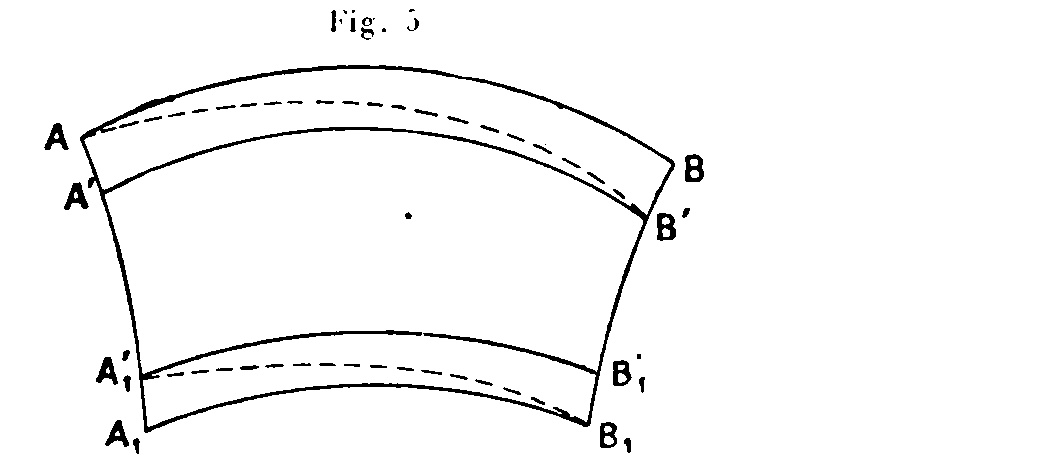
\includegraphics[width=0.55\textwidth]{fig5_scan.jpg}
\end{center}

Soit $A'$ un point assez voisin de A pour que l’arc $AA'$ soit sans contact et que la caractéristique $A'B'$ aille couper $BB_1$ en un point $B'$ tel que $BB'$ soit sans contact.

Supposons de même que $A'_1B'_1$ soit un arc de caractéristique et que $A_1A'_1$, $B_1B'_1$ soient sans contact.

On pourra mener, d’après le théorème précédent, des arcs algébriques $AB'$, $A'_1B_1$ sans contact.

Le nombre des contacts du cycle algébrique
\[
AB'B_1A'_1A
\]
doit être pair.

Or, les caractéristiques AB, $A_1B_1$ touchent le cycle en A et en $B_1$; les caractéristiques $A'B'$ et $A'_1B'_1$ le traversent en $B'$ et en $A'_1$. Donc les quatre points anguleux comptent pour un nombre pair de contacts. Donc on a
\[
\begin{aligned}
&\text{nombre des contacts } AB' + \text{nombre des contacts } B'B_1\\
&\quad + \text{nombre des contacts } B_1A'_1 + \text{nombre des contacts } A'_1A \equiv 0 \pmod 2,
\end{aligned}
\]
ou, ce qui revient au même,
\[
\text{nombre des contacts } AA_1 + \text{nombre des contacts } BB_1 \equiv 0 \pmod 2.
\]
\hfill\mbox{C. Q. F. D.}

\emph{Théorème X.} --- \emph{Si un arc de caractéristique qui ne passe par aucun point singulier est sous-tendu par un arc de courbe, le nombre des contacts de cet arc de courbe est impair.}

En effet, soit $\mathrm F=0$ l’équation de l’arc sous-tendant. Considérons la fonction $\mathrm F$; cette fonction passe, par exemple, du positif au négatif quand le point $(x,y)$, décrivant la caractéristique, passe par l’une des extrémités de l’arc sous-tendant, et du négatif au positif quand il passe par l’autre extrémité de cet arc. C’est dire que, quand le point $(x,y)$ décrit l’arc donné de caractéristique, la fonction $\mathrm F$ passe par un nombre impair de maxima et de minima.

Or, ces maxima et ces minima sont donnés par l’équation
\[
\varphi=X\frac{d\mathrm F}{dx}+Y\frac{d\mathrm F}{dy}=0;
\]
c’est dire que l’arc de caractéristique coupe en un nombre impair de points la courbe $\varphi=0$.

Or, cette courbe, qui est algébrique, coupe en un nombre pair de points le cycle H formé par l’arc de caractéristique et l’arc sous-tendant; donc elle coupe l’arc sous-tendant en un nombre impair de points.

Donc le nombre des contacts de cet arc est impair. \hfill\mbox{C. Q. F. D.}

\emph{Remarque I.} --- Si l’arc de caractéristique passe par un col, comment faudra-t-il modifier le théorème?

Le col appartient évidemment à la courbe $\varphi=0$, mais il n’est un maximum ou un minimum de $\mathrm F$ qu’à la condition que l’arc de caractéristique présente en ce point un point anguleux.

En effet, supposons d’abord qu’il n’y ait pas de point anguleux. Les courbes $\mathrm F=\mathrm F(x_0,y_0)$ et $\varphi=0$ traverseront toutes deux, en général, le cycle H, c’est-à-dire que le col sera un point simple d’intersection du cycle et de $\varphi=0$, sans correspondre à un maximum ou à un minimum de $\mathrm F$.

Si, au contraire, il y a un point anguleux, l’une des courbes $\varphi=0$, $\mathrm F=0$ traversera le cycle H, pendant que l’autre le touchera, de telle sorte que, ou bien le col sera un point simple d’intersection de H et de $\varphi=0$, et en même temps un maximum de $\mathrm F$, ou bien il sera un point double de H et de $\varphi=0$ sans être un maximum de $\mathrm F$.

Donc, si l’arc de caractéristique passe par un col et n’y a pas de point anguleux, le nombre des contacts de l’arc sous-tendant est pair.

Si l’arc de caractéristique passe par un col et y a un point anguleux, le nombre de ces contacts est impair.

\emph{Remarque II.} --- On démontrerait de même que, si un arc de caractéristique ne passe par aucun point singulier, tout arc de courbe qui le sur-tend a un nombre de contacts pair.

\emph{Contacts des systèmes topographiques.} --- Si l’on considère un système topographique algébrique, les contacts de ce système formeront une courbe algébrique.

On distinguera les contacts intérieurs et extérieurs du système topographique, selon que dans le voisinage de ces contacts la caractéristique qui y passe reste intérieure ou extérieure au cycle qu’elle touche, parmi ceux du système topographique.

La courbe des contacts sera donc divisée en un certain nombre d’arcs qui seront les arcs des contacts intérieurs et ceux des contacts extérieurs.

Ces arcs seront séparés :

\begin{enumerate}[label=\arabic*°]
\item Par les points singuliers;
\item Par les points où la courbe des contacts touche un des cycles du système topographique.
\end{enumerate}


\ornament
\begin{center}
{\Large CHAPITRE V.}\\[0.4em]
{\small THÉORIE DES CONSÉQUENTS.}
\end{center}
\shortline

\emph{Convention fondamentale.} --- Considérons une demi-caractéristique quelconque; nous la prolongerons indéfiniment, si l'on peut le faire sans rencontrer un point singulier; si, au contraire, en suivant la demi-caractéristique, nous arrivons à un nœud, nous l'arrêterons à un nœud; si nous arrivons à un col, trois chemins s'ouvriront devant nous quand nous voudrons continuer à suivre la caractéristique, le premier dans le prolongement du chemin suivi jusqu'alors, les deux autres à droite et à gauche; nous conviendrons de suivre l'un des chemins de droite ou de gauche, sans jamais prendre celui qui est directement devant nous. Par exemple, nous considérerons OB ou OD (fig. 6) et non pas OC, comme le prolongement de AO.

\figscan{6}{0.48\textwidth}

De cette façon, on peut dire que dans le voisinage d'un col il y a quatre caractéristiques collées l'une contre l'autre, et ayant deux à deux une branche commune : ce sont les caractéristiques AOB, BOC, COD, DOA.

\emph{Définition des conséquents.} --- Soit
\[
x=\varphi(t),\qquad y=\psi(t)
\]
un arc algébrique sans contact; $\varphi$ et $\psi$ sont des fonctions algébriques de $t$, et n'ont qu'une seule valeur pour chaque valeur de $t$. Les extrémités de l'arc correspondront aux valeurs de $t$,
\[
t=\alpha,\qquad t=\beta.
\]

Un pareil arc, sans contact, aura deux côtés que nous appellerons sa droite et sa gauche; un point infiniment voisin de l'arc AB pourra, en effet, être à droite ou à gauche de cet arc. Par exemple, le point $m$ sera à gauche de l'arc AB (fig. 7), le point $m'$ à droite de l'arc AB, parce qu'on ne peut passer de l'un à l'autre sans traverser l'arc AB, ou sans s'éloigner de cet arc à une distance finie, ou sans passer par un cercle de rayon infiniment petit tracé avec A ou avec B comme centre.

\figscan{7}{0.44\textwidth}

Ceci posé, considérons un point quelconque $\mathrm M_0$ de l'arc AB (fig. 8); de ce point partent deux demi-caractéristiques, l'une vers la gauche, l'autre vers la droite de l'arc AB; considérons celle de gauche.

\figscan{8}{0.55\textwidth}

Il pourra se présenter plusieurs cas :
\begin{enumerate}[label=\arabic*°]
\item Cette demi-caractéristique peut se prolonger indéfiniment, sans qu'on rencontre de nouveau l'arc AB.
\item Cette demi-caractéristique finit en tournant autour d'un foyer, avant d'avoir rencontré de nouveau l'arc AB.
\item Elle aboutit à un nœud où nous devons l'arrêter, d'après la convention fondamentale, et cela avant d'avoir rencontré de nouveau l'arc AB.
\end{enumerate}

Dans ces trois premiers cas, nous dirons que \emph{le point $\mathrm M_0$ n'a pas de conséquent.}

\begin{enumerate}[label=\arabic*°,start=4]
\item La demi-caractéristique vient rencontrer l'arc AB en $\mathrm M_1$ avant d'avoir passé par un point singulier. Nous dirons alors que \emph{le point $\mathrm M_1$ est le conséquent du point $\mathrm M_0$.}
\item La demi-caractéristique aboutit à un col avant d'être arrivée à rencontrer de nouveau l'arc AB. Dans ce cas, d'après la convention fondamentale, il faut tourner soit à droite, soit à gauche, et chacun de ces deux chemins peut nous conduire ou ne pas nous conduire à rencontrer de nouveau l'arc AB. Le point $\mathrm M_0$ peut alors avoir $0$, $1$ ou $2$ conséquents.
\end{enumerate}

Il peut enfin arriver que la demi-caractéristique rencontre deux cols ou plus encore, et dans ce cas le point $\mathrm M_0$ pourrait avoir plus de deux conséquents.

Si, en partant du point $\mathrm M_0$, au lieu de considérer la demi-caractéristique de gauche, on avait envisagé celle de droite, on aurait pu arriver à un point $\mathrm M'$ situé sur l'arc AB.

\emph{Ce point $\mathrm M'$ s'appellera l'antécédent du point $\mathrm M_0$.}

Dans ces conditions, le point $\mathrm M_0$ sera lui-même l'antécédent de son conséquent $\mathrm M_1$.

Si $t_0$ et $t_1$ sont des valeurs de $t$ qui correspondent à $\mathrm M_0$ et à $\mathrm M_1$, la loi de conséquence sera la relation qui lie $t_0$ à $t_1$.

\emph{Théorème XI.} --- \emph{Si $t_0=t_1$, la caractéristique est un cycle. Si $t_0\gtrless t_1$, la caractéristique est une spirale.}

En effet, la première partie de l'énoncé est une véritable tautologie. La seconde se démontre aisément de la manière suivante :

Remarquons d'abord que l'arc $\mathrm M_0\mathrm D\mathrm M_1$ (fig. 9) sur-tend l'arc $\mathrm M_0\mathrm C\mathrm M_1$ de la caractéristique, car il est sans contact.

De plus, cet arc $\mathrm M_0\mathrm D\mathrm M_1$ ne peut rencontrer la caractéristique en aucun autre point que $\mathrm M_0$ et $\mathrm M_1$. Car des arcs tels que $\mathrm M_1\mathrm F\mathrm M_2$, $\mathrm M_0\mathrm H\mathrm M_3$ seraient sous-tendus par les arcs $\mathrm M_1\mathrm M_2$, $\mathrm M_0\mathrm M_3$, ce qui est impossible, puisque ces arcs sont supposés sans contact.

\figscan{9}{0.6\textwidth}

Ceci posé, par le point $\mathrm N_0$ infiniment voisin de $\mathrm M_0$ et à gauche de ce dernier, on pourra mener un arc de caractéristique $\mathrm N_0\mathrm E\mathrm N_1$ qui viendra rencontrer l'arc $\mathrm M_0\mathrm M_1$ en un point $\mathrm N_1$ infiniment voisin de $\mathrm M_1$ et à gauche de ce dernier, car il ne pourrait passer à droite sans couper la caractéristique $\mathrm M_0\mathrm C\mathrm M_1$, ce qui est impossible.

Le cycle $\mathrm N_1\mathrm M_0\mathrm N_0\mathrm E\mathrm N_1$ ne rencontre donc la caractéristique $\mathrm M_0\mathrm C\mathrm M_1$ qu'en un seul point qui est $\mathrm M_0$. Donc, cette caractéristique est une spirale. \hfill\mbox{C. Q. F. D.}

\emph{Théorème XII.} --- \emph{Toute caractéristique qui n'aboutit pas à un nœud est un cycle ou une spirale.}

En effet, si cette caractéristique ne rencontre aucun cycle algébrique en une infinité de points, elle est un cycle, en vertu du théorème I.

Si, au contraire, elle rencontre un cycle algébrique en une infinité de points, comme ce cycle se compose d'un nombre fini d'arcs sans contact, elle rencontrera l'un de ces arcs, et aura contact en plus d'un point, c'est-à-dire que l'un des points d'intersection aura un conséquent.

S'il se confond avec son conséquent, la caractéristique est un cycle; s'il ne se confond pas avec son conséquent, la caractéristique est une spirale, en vertu du théorème XI.

Le théorème est donc démontré.

\emph{Théorème XIII.} --- \emph{Si $\mathrm M_0$ ne correspond pas à une caractéristique passant par un col, et s'il a un conséquent $\mathrm M_1$; si $t_1=\varphi_1(t_0)$ est la loi de conséquence, la fonction $\varphi_1$ est holomorphe pour les valeurs de $t_0$ voisines de celle qui correspond à $\mathrm M_0$.}

En effet, nous avons supposé au début que si
\[
x=\varphi(t),\qquad y=\psi(t)
\]
sont les équations de l'arc sans contact, $\varphi$ et $\psi$ sont des fonctions holomorphes de $t$ dans le voisinage de la valeur de $t$ qui correspond à $\mathrm M_0$, et aussi de celle qui correspond à $\mathrm M_1$.

Supposons que l'on cherche une intégrale de l'équation aux différences partielles
\[
X\frac{dz}{dx}+Y\frac{dz}{dy}=0,
\]
qui soit assujettie à se réduire identiquement à $t_0$, quand on y fait
\[
x=\varphi(t_0),\qquad y=\psi(t_0).
\]

Cette intégrale représente une surface qui passe par la courbe gauche,
\[
x=\varphi(z),\qquad y=\psi(z).
\]

Dans le voisinage du point $\mathrm M_0$, cette intégrale est holomorphe en $x$ et en $y$; car l'arc
\[
x=\varphi(t_0),\qquad y=\psi(t_0)
\]
ne touche pas une caractéristique.

Elle sera de même holomorphe en $x$ et en $y$ tout le long de la caractéristique qui passe par le point $\mathrm M_0$, à moins que cette caractéristique ne passe par un point singulier. Or, nous avons supposé que cette caractéristique allait passer par le point $\mathrm M_1$ sans avoir rencontré aucun point singulier. Dans le voisinage du point $\mathrm M_1$, $z$ est donc fonction holomorphe de $x$ et de $y$; et, si l'on y fait
\[
x=\varphi(t_1),\qquad y=\psi(t_1),
\]
$z$ devient fonction holomorphe de $t_1$, dans le voisinage de la valeur de $t_1$, qui correspond à $\mathrm M_1$.

Or, $z$ n'est autre chose que $t_0$. Donc, $t_0$ est fonction holomorphe de $t_1$. On démontrerait identiquement, de la même manière, que $t_1$ est fonction holomorphe de $t_0$ dans le voisinage de la valeur de $t_0$ qui correspond à $\mathrm M_0$.

\emph{Corollaire I.} --- La fonction $t_1=\varphi_1(t_0)$, qui exprime la loi de conséquence, ne peut offrir de discontinuité que pour les valeurs de $t_0$ qui correspondent à des caractéristiques passant par des cols.

\emph{Corollaire II.} --- Si l'on divise l'arc sans contact AB en arcs partiels, tels que tous les points de chacun de ces arcs aient un conséquent, ou qu'aucun n'en ait, les extrémités de ces arcs partiels seront des points ayant pour conséquent une extrémité de l'arc sans contact AB, ou correspondant à des caractéristiques passant par des cols.

\emph{Corollaire III.} --- Si les extrémités de l'arc sans contact correspondent aux valeurs
\[
t=\alpha,
\qquad
 t=\beta;
\]
si, pour aucune valeur de $t$ telle que
\[
\alpha<t<\beta,
\]
la caractéristique correspondante ne passe pas par un col;

si, pour toutes les valeurs de $t$, telles que ($\alpha_1$ et $\beta_1$ étant des constantes données), on ait
\[
\alpha<\alpha_1<t<\beta_1<\beta,
\]
la caractéristique correspondante est un cycle;

les caractéristiques qui correspondent à une valeur quelconque de $t$ comprise entre $\alpha$ et $\beta$ sont toutes des cycles.

\emph{Théorème XIV.} --- \emph{La valeur de $\dfrac{dt_1}{dt_0}$ est toujours positive.}

En effet, soit AB l'arc sans contact (fig. 11), soit $\mathrm M_0\mathrm M_1$ une caractéristique,

\figscan{10}{0.48\textwidth}

soit $\mathrm N_0$ un point infiniment voisin de $\mathrm M_0$ et situé à droite de ce point. Soit $\mathrm N_0\mathrm N_1$ la caractéristique qui passe par ce point. Le point $\mathrm N_1$ est infiniment voisin de $\mathrm M_1$; je dis qu'il est à droite de ce point. Car, pour qu'il fût à gauche, il faudrait que la caractéristique $\mathrm N_0\mathrm N_1$ sortît du cycle $\mathrm M_0\mathrm H\mathrm M_1\mathrm N_0\mathrm M_0$ quand on la prolonge au delà de $\mathrm N_1$, c'est-à-dire que l'arc de caractéristique $\mathrm N_0\mathrm N_1$ fût sous-tendu par l'arc $\mathrm N_0\mathrm N_1$, ce qui est impossible, puisque cet arc est sans contact.

\emph{Étude de la courbe de conséquence.} --- Si l'on considère les quantités $t_0$ et $t_1$ comme les coordonnées d'un point, la loi de conséquence
\[
t_1=\varphi_1(t_0)
\]
représente une courbe. Cette courbe est comprise tout entière dans le carré
\[
\begin{array}{ll}
t_0=\alpha, & t_1=\alpha,\\
t_0=\beta, & t_1=\beta.
\end{array}
\]

\emph{Premier cas.} --- A aucune valeur de $t$ comprise entre $\alpha$ et $\beta$ ne correspond de caractéristique allant passer par un col.

Dans ce cas, la courbe de conséquence est continue; elle ne rencontre qu'en un point les parallèles aux axes; en suivant la courbe dans un certain sens convenable, on va constamment en s'éloignant de ces deux axes.

C'est dire que si KLCD est le carré (fig. 11)
\[
\begin{array}{ll}
t_0=\alpha, & t_1=\alpha,\\
t_0=\beta, & t_1=\beta,
\end{array}
\]
la courbe présente des formes telles que
\[
\mathrm{AB},\quad \mathrm{CD},\quad \mathrm{EF},\quad \mathrm{GH}.
\]

\figscan{11}{0.45\textwidth}

Elle représentera la forme CD quand les valeurs $\alpha$ et $\beta$ de $t_0$ correspondront à des cycles, pendant qu'aucune valeur de $t_0$ comprise entre $\alpha$ et $\beta$ ne correspondra à un cycle.

\emph{Deuxième cas.} --- Supposons qu'à certaines valeurs de $\gamma_0$, $\gamma'_0$, \ldots{} de $t_0$ comprises entre $\alpha$ et $\beta$ correspondent des caractéristiques allant passer par un col;

que, de plus, aux valeurs $\alpha$ et $\beta$ correspondent des cycles; qu'à aucune valeur intermédiaire ne corresponde un cycle :

De tous les cols partent quatre branches de caractéristiques; certaines de ces branches viennent rencontrer l'arc sans contact donné; d'autres ne le font pas.

Supposons d'abord que toutes celles de ces branches qui viennent rencontrer l'arc sans contact donné partent d'un seul et même col :

$1^\circ$ Il est impossible que les quatre branches issues d'un même col aillent rencontrer l'arc sans contact. Soit, en effet, AB (fig. 12) l'arc sans contact

\figscan{12}{0.5\textwidth}

donné. Soit C le col donné; soient $\mathrm C\mathrm M_0$, $\mathrm C\mathrm M_1$, $\mathrm C\mathrm N_0$, $\mathrm C\mathrm N_1$ les quatre branches de caractéristiques qui partent de ce col, de telle façon que $\mathrm M_1\mathrm C\mathrm M_0$, $\mathrm N_1\mathrm C\mathrm N_0$, ne forment pas de point anguleux.

D'après le théorème X, remarque I, la portion $\mathrm M_0\mathrm M_1$ de l'arc AB sous-tend la caractéristique $\mathrm M_0\mathrm C\mathrm M_1$.

Les deux arcs $\mathrm A\mathrm M_0$, $\mathrm M_1\mathrm B$ sont donc d'un même côté du cycle $\mathrm M_0\mathrm M_1\mathrm C\mathrm M_0$; appelons ce côté du cycle l'extérieur du cycle. Les deux branches de courbe $\mathrm C\mathrm N_0$, $\mathrm C\mathrm N_1$ sont l'une à l'extérieur, l'autre à l'intérieur du cycle $\mathrm M_0\mathrm M_1\mathrm C\mathrm M_0$. Soit $\mathrm C\mathrm N_1$ celle qui est à l'intérieur; elle ne pourrait rencontrer l'arc AB qu'entre $\mathrm M_0$ et $\mathrm M_1$, et du même côté que les branches de courbe $\mathrm C\mathrm M_0$, $\mathrm C\mathrm M_1$, de telle sorte que l'arc algébrique $\mathrm M_1\mathrm N_1$ sous-tendrait l'arc de caractéristique $\mathrm M_1\mathrm C\mathrm N_1$, ce qui est impossible d'après le théorème X.

\emph{Remarque I.} --- L'hypothèse que nous avons faite en commençant est donc absurde. \hfill\mbox{C. Q. F. D.}

$2^\circ$ Il peut se faire que trois des branches issues d'un même col aillent rencontrer l'arc sans contact. Dans ce cas, ou bien il y a un point qui a deux conséquents et les points situés entre ces deux conséquents n'ont pas d'antécédent; ou bien il y a un point qui a deux antécédents, et les points situés entre ces deux antécédents n'ont pas de conséquent.

De telle façon que la courbe de conséquence affecte soit la forme CHFD, soit la forme CABD (fig. 13).

\figscan{13}{0.42\textwidth}

$3^\circ$ Il ne peut se faire que deux ou une seulement des branches issues d'un même col aillent rencontrer l'arc sans contact.

En effet, supposons d'abord qu'il y ait deux branches de caractéristiques $\mathrm C\mathrm M_0$ et $\mathrm C\mathrm M_1$ qui rencontrent AB, et que $\mathrm M_0\mathrm C\mathrm M_1$ (fig. 14) présente un point anguleux

\figscan{14}{0.48\textwidth}

en C. Un point infiniment voisin de $\mathrm M_0$ aura un conséquent s'il est à droite de $\mathrm M_0$, et n'en aura pas s'il est à gauche. Donc, d'après le corollaire II du théorème XIII, les points de l'arc $\mathrm M_0\mathrm A$ n'auront donc pas de conséquent. Un point infiniment voisin de A n'aurait donc pas de conséquent, ce qui est absurde puisque A est son propre conséquent. De même, si l'on supposait que $\mathrm M_1\mathrm C\mathrm M_0$ ne présente pas de point anguleux, ou que $\mathrm C\mathrm M_1$ ne rencontre pas l'arc AB, on arriverait à ce résultat absurde qu'un point infiniment voisin de A n'a pas de conséquent. Les hypothèses faites au début sont donc également absurdes. \hfill\mbox{C. Q. F. D.}

Nous n'examinerons pas en détail les cas où les branches de caractéristiques qui viennent rencontrer l'arc sans contact sont issues de plusieurs cols différents. La discussion se ferait d'après les mêmes principes, elle serait seulement plus longue. Citons seulement quelques exemples de combinaisons possibles\footnote{Il ressort du texte que l'auteur avait en vue un second exemple, correspondant à la courbe représentative CEFGHD. Dans ce cas, l'arc sans contact est rencontré par trois branches de caractéristiques issues d'un premier col, et par trois branches issues d'un second col. (R. G.)}.

$1^\circ$ \emph{Courbe} CABD (fig. 15). --- L'arc sans contact est rencontré par deux

\figscan{15}{0.42\textwidth}

branches de caractéristiques issues d'un premier col $\lambda$ et par deux branches issues d'un second col $\mu$. Ces deux systèmes de deux branches de caractéristiques présentent chacun un point anguleux, l'un en $\lambda$, l'autre en $\mu$.

Si l'on fait varier $t_0$ depuis $\alpha$ jusqu'à la valeur qui correspond au point A et à la caractéristique qui passe en $\lambda$, on a un conséquent; ensuite $t_0$ variant depuis la valeur qui correspond au point A jusqu'à celle qui correspond au point B et à la caractéristique qui passe en $\mu$, on n'a plus de conséquent; et l'on en a un de nouveau quand $t_0$ varie depuis la valeur qui correspond à B jusqu'à $\beta$.

\ornament
\begin{center}
{\Large CHAPITRE VI.}\\[0.4em]
{\small THÉORIE DES CYCLES LIMITES.}
\end{center}
\shortline

D'après ce que nous avons vu plus haut, les caractéristiques peuvent se diviser en quatre catégories :
\begin{enumerate}[label=\arabic*°]
\item Les cycles;
\item Les spirales que l'on peut suivre indéfiniment dans les deux sens sans aboutir à un nœud ou sans tourner autour d'un foyer, et sans revenir au point de départ;
\item Les caractéristiques que l'on peut suivre indéfiniment dans un sens sans rencontrer un nœud ou se rapprocher d'un foyer, mais qui, dans l'autre sens, aboutissent à un nœud ou se rapprochent indéfiniment d'un foyer;
\item Celles qui aboutissent de part et d'autre à un nœud ou à un foyer.
\end{enumerate}

D'après les mêmes principes, les \emph{demi-caractéristiques} se divisent en quatre catégories :
\begin{enumerate}[label=\arabic*°]
\item Les cycles;
\item Les demi-spirales que l'on suit sur un arc infini sans arriver à un nœud ou à un foyer et sans revenir au point de départ;
\item Les demi-caractéristiques qui aboutissent à un nœud;
\item Celles qui tournent indéfiniment autour d'un foyer.
\end{enumerate}

D'après le théorème I, les demi-caractéristiques de la seconde catégorie rencontrent certains cycles algébriques, et par conséquent certains arcs algébriques sans contact en une infinité de points.

Soit AB un de ces arcs algébriques sans contact.

Soit $\mathrm M_0$ (fig. 16) le point d'où est issue la demi-caractéristique considérée.

\figscan{16}{0.62\textwidth}

Soit $\mathrm M_1$ le conséquent de $\mathrm M_0$, et supposons que $\mathrm M_1$ soit à droite de $\mathrm M_0$.

Soient $\mathrm M_2$ le conséquent de $\mathrm M_1$, $\mathrm M_3$ celui de $\mathrm M_2$, etc.; $\mathrm M_2$ sera à droite de $\mathrm M_1$, $\mathrm M_3$ sera à droite de $\mathrm M_2$, etc.

En général, $\mathrm M_{n+1}$ sera à droite de $\mathrm M_n$, et comme, quelque grand que soit $n$, $\mathrm M_n$ est toujours sur l'arc AB, $\mathrm M_n$ tendra vers une limite quand $n$ augmentera indéfiniment. Soit H cette limite.

Le conséquent de $\mathrm M_n$, quand $n$ est infiniment grand, est infiniment rapproché de $\mathrm M_n$. Donc H est son propre conséquent; donc la caractéristique qui passe par H est un cycle; nous l'appellerons \emph{cycle limite} de la demi-caractéristique donnée. On peut suivre sur la caractéristique qui passe par $\mathrm M_0$ un arc assez grand pour se rapprocher autant que l'on veut du point H.

Soit HK un arc de la caractéristique qui passe par le point H. Soit CD un arc algébrique passant par K.

On pourra prendre $n$ assez grand pour que l'arc de caractéristique issu de $\mathrm M_n$ aille rencontrer CD.

Supposons, par exemple, que l'arc issu de $\mathrm M_2$ aille rencontrer CD en $\mathrm N_2$. L'arc issu de $\mathrm M_3$ ira rencontrer CD en $\mathrm N_3$, ... l'arc issu de $\mathrm M_n$, en un point $\mathrm N_n$.

$\mathrm N_3$ sera à droite de $\mathrm N_2$, ..., $\mathrm N_{n+1}$ sera à droite de $\mathrm N_n$. De sorte que la demi-caractéristique donnée rencontrera CD en une infinité de points $\mathrm N_2$, $\mathrm N_3$, ..., $\mathrm N_n$, et que $\mathrm N_n$ tendra vers K quand $n$ augmentera indéfiniment.

En résumé, toute demi-caractéristique de la seconde catégorie a un cycle limite.

Tout arc algébrique, si petit qu'il soit, qui coupe ce cycle, coupe la demi-caractéristique en une infinité de points.

On peut trouver un point de la demi-caractéristique qui soit aussi rapproché qu'on voudra d'un point quelconque de son cycle limite.

Soit AB (fig. 17) un arc algébrique sans contact. Supposons qu'à aucun

\figscan{17}{0.45\textwidth}

point M situé entre A et B ne corresponde une caractéristique allant passer par un col; qu'au point $\mathrm M_0$ corresponde un cycle limite, et qu'à aucun point M différent de $\mathrm M_0$, situé entre A et B, ne corresponde un cycle limite. Toute caractéristique qui rencontre AB aura pour cycle limite le cycle qui passe par $\mathrm M_0$.

Si l'on considère un cycle limite C (fig. 18) qui ne passe pas par un col et qui passe par un point $\mathrm M_0$, on pourra mener par $\mathrm M_0$ un arc algébrique AB assez petit pour qu'il soit sans contact; pour qu'entre A et $\mathrm M_0$, ou entre $\mathrm M_0$ et B il n'y ait aucun point auquel corresponde une caractéristique passant par un col ou un cycle limite. Toutes les caractéristiques qui rencontrent AB ont alors C

\figscan{18}{0.47\textwidth}

pour cycle limite, de sorte que C est le cycle limite de deux séries de caractéristiques situées l'une à l'intérieur du cycle, l'autre à l'extérieur.

Voyons ce qui se passe quand C va passer par un col.

Soient H le col, HA, HB, HC, HD les quatre branches de caractéristiques issues de ce col. Supposons que deux de ces branches, HA et HB par exemple, aillent aboutir à un même point M, de façon à former un cycle HAMBH; ce cycle sera toujours cycle limite de courbes telles que $\alpha\alpha$; l'inspection de la figure le démontre (fig. 19).

\figscan{19}{0.75\textwidth}

Considérons, au contraire, la courbe $\beta\beta$; il est aisé de voir que, si les branches de courbe HC, HD ne vont pas aboutir en un même point N, le cycle HAMBH n'est pas cycle limite de $\beta\beta$.

Si, au contraire, HC et HD vont se réunir en N, $\beta\beta$ a pour cycle limite le polycycle
\[
\mathrm{HAMBHDNCH}.
\]

\emph{Théorème XV.} --- \emph{A l'intérieur et à l'extérieur d'un cycle limite quelconque, il y a toujours au moins un foyer ou un nœud.}

Pour démontrer ce théorème nous allons appeler \emph{tangences d'un cycle} les points où il touche un des grands cercles $x=\mathrm{const.}$

Les tangences seront directes si, dans le voisinage du point de contact, le grand cercle tangent reste à l'extérieur du cycle. Elles seront inverses dans le cas contraire.

Nous démontrerons ensuite les deux lemmes suivants :

\emph{Lemme I.} --- \emph{Si les points d'intersection de l'équateur avec le grand cercle $x=0$, points que nous appellerons $m$, $m'$, sont tous deux à l'extérieur d'un cycle, l'excès du nombre des tangences directes de ce cycle sur le nombre de ses tangences inverses est de 2.}

Si les points $m$, $m'$ sont tous deux à l'intérieur du cycle, cet excès est de $-2$.

Si les points $m$, $m'$ sont l'un à l'extérieur, l'autre à l'intérieur, cet excès est de 0.

En effet, on peut passer d'un cycle quelconque A à un autre cycle également quelconque B par voie de déformation continue, c'est-à-dire en passant du cycle A à un cycle qui en diffère infiniment peu, A', et ensuite par une série de cycles C infiniment peu différents les uns des autres, on arrivera à un cycle B', infiniment peu différent de B.

Dans ces déformations successives, une tangence directe ne se transformera jamais en une tangence inverse, ni une tangence inverse en une tangence directe, car cela ne pourrait avoir lieu que si l'un des grands cercles $x=\mathrm{const.}$ devenait osculateur à l'un des cycles; dans ce cas, ce serait que deux tangences, l'une directe et l'autre inverse, seraient venues à se confondre, et, dans ce cas, elles disparaîtraient en général pour un des cycles infiniment voisins de C.

L'excès qu'il s'agit d'évaluer dans ce lemme ne peut se modifier dans ces déformations continues du cycle que si deux des tangences viennent à se confondre, puis à disparaître. Or cela peut arriver dans deux cas :

$1^\circ$ Quand l'un des cycles C vient à passer par l'un des points $m$, $m'$; mais nous supposerons : $1^\circ$ que les points $m$, $m'$ sont tous deux à l'intérieur de A et tous deux à l'extérieur de B; $2^\circ$ ou que les points $m$, $m'$ sont tous deux à l'extérieur de A et à l'extérieur de B; $3^\circ$ ou que $m$ soit à l'extérieur de A et de B pendant que $m'$ est à l'intérieur de ces deux cycles; et, par conséquent, on aura pu toujours choisir la série des cycles C qui permettent de passer du cycle A au cycle B, de telle sorte qu'aucun des cycles C ne passe ni par $m$, ni par $m'$.

$2^\circ$ Cela peut arriver encore si l'un des cycles C devient osculateur à l'un des cercles $x=\mathrm{const.}$ Mais, dans ce cas, c'est une tangence directe et une tangence inverse qui se confondent et disparaissent. L'excès à évaluer n'est donc pas modifié.

Donc cet excès est le même pour A et pour B.

Mais supposons que A soit un cycle convexe quelconque, et B le cycle donné.

L'excès en question sera de 2 pour A si $m$ et $m'$ sont à l'extérieur de A; il sera de $-2$ s'ils sont tous deux à l'intérieur, et 0 s'ils sont l'un à l'intérieur et l'autre à l'extérieur.

L'excès en question sera donc, pour B, de 2, de $-2$ et de 0 dans les mêmes conditions.

Le lemme est donc démontré.

\emph{Lemme II.} --- \emph{Si l'on parcourt un cycle de manière à avoir toujours l'intérieur à sa gauche et que l'on observe les variations du coefficient angulaire $\frac{dy}{dx}$, on observera qu'à chaque tangence directe, $\frac{dy}{dx}$ sautera de $+\infty$ à $-\infty$ si l'on est dans le premier hémisphère, et de $-\infty$ à $+\infty$ si l'on est dans le second hémisphère, et que c'est le contraire pour les tangences inverses.}

\emph{Démonstration du théorème.} --- Supposons d'abord que le cycle limite considéré soit tel que les deux points $m$ et $m'$ soient d'un même côté de ce cycle, côté que nous appellerons l'\emph{extérieur du cycle}.

Soient :

$\nu$ le nombre des nœuds et des foyers contenus à l'intérieur du cycle;

$\nu'$ le nombre des nœuds et des foyers situés à l'extérieur du cycle;

$\gamma$ et $\gamma'$ le nombre des cols situés à l'intérieur et à l'extérieur de ce cycle.

On a
\[
\nu+\nu'-\gamma-\gamma'=2.
\]

Le cycle coupe l'équateur en un certain nombre de points, de telle façon qu'on peut le partager en un certain nombre de cycles secondaires situés les uns tout entiers dans le premier hémisphère, les autres tout entiers dans le second hémisphère, et formés à l'aide d'arcs du cycle primitif et d'arcs de l'équateur.

Supposons, pour fixer les idées, que le cycle donné soit le cycle ALDKCGBHA, qui coupe l'équateur aux points A, B, C, D (fig. 20). Le cycle se décompose

\figscan{20}{0.62\textwidth}

en trois cycles secondaires :
\[
\mathrm{AEBHA},\qquad \mathrm{CFDKC},\qquad \mathrm{CGBEALDFC}.
\]

Or, d'après le théorème IV, on a
\[
-(\nu-\gamma)=\operatorname{ind.}\mathrm{AEBHA}+\operatorname{ind.}\mathrm{CFDKC}+\operatorname{ind.}\mathrm{CGBEALDFC}.
\]

Soient, maintenant, $\alpha$, $\alpha'$, $\alpha''$, $\alpha'''$ le nombre des tangences directes des arcs AHB, CKD, CGB, ALD; $\beta$, $\beta'$, $\beta''$, $\beta'''$ le nombre de leurs tangences inverses; soient $\lambda$ et $\lambda'$ le nombre de fois que $\frac{Y}{X}$ saute de $-\infty$ à $+\infty$ quand on parcourt les arcs AEB et CFD; $\mu$ et $\mu'$ le nombre de fois que $\frac{Y}{X}$ saute de $+\infty$ à $-\infty$ quand on parcourt les arcs AEB et CFD; on a, en vertu du lemme II et en remarquant que tout le long du cycle donné on a
\[
\frac{dy}{dx}=\frac{Y}{X},
\]
\[
\begin{aligned}
2\operatorname{ind.}\mathrm{AEBHA}&=-\alpha+\lambda-\mu+\beta,\\
2\operatorname{ind.}\mathrm{CFDKC}&=-\alpha'+\lambda'-\mu'+\beta',\\
2\operatorname{ind.}\mathrm{CGBEAL}&=-\alpha''-\alpha'''+\beta''+\beta'''-\lambda-\lambda'+\mu+\mu'.
\end{aligned}
\]
d'où
\[
-(2\nu-2\gamma)=\beta+\beta'+\beta''+\beta'''-\alpha-\alpha'-\alpha''-\alpha''',
\]
ou, d'après le lemme I,
\[
-(2\nu-2\gamma)=-2,\qquad \nu-\gamma=1.
\]
On a donc aussi
\[
\nu'-\gamma'=1,
\]
d'où
\[
\nu>0,\qquad \nu'>0.
\]
\hfill\mbox{C. Q. F. D.}

Dans les cas où les points $m$, $m'$ sont de part et d'autre du cycle, la difficulté est facile à tourner. En effet, on trouvera toujours sur la sphère deux points diamétralement opposés qui soient d'un même côté du cycle, et il suffira d'un changement de variables pour retomber sur le cas précédent.

Si l'on ne trouve pas sur la sphère deux points diamétralement opposés qui soient d'un même côté du cycle, c'est que les points du cycle sont deux à deux diamétralement opposés, c'est-à-dire que le cycle est symétrique à lui-même par rapport au centre de la sphère, et alors le théorème est évident par lui-même.

\emph{Théorème XVI.} --- \emph{Un cycle algébrique qui passe par tous les nœuds et par tous les foyers rencontre tous les cycles limites.}

En effet, soit un cycle limite C quelconque; il contient certains nœuds et certains foyers à son intérieur, certains nœuds et certains foyers à l'extérieur.

Il y a donc des points du cycle algébrique donné qui sont à l'extérieur de C, et d'autres qui sont à l'intérieur, c'est-à-dire que le cycle algébrique donné rencontre C. \hfill\mbox{C. Q. F. D.}

\emph{Corollaire.} --- Tout cycle algébrique qui passe par tous les nœuds et par tous les foyers rencontre toutes les caractéristiques.

\emph{Théorème XVII.} --- \emph{Les cycles limites sont en nombre fini, pourvu qu'aucun d'eux ne passe par un col.}

En effet, faisons passer un cycle algébrique C par tous les nœuds et par tous les foyers. Soient
\[
x=\varphi(t),\qquad y=\psi(t)
\]
les équations de ce cycle C.

Ce cycle C, rencontrant tous les cycles limites, aurait une infinité de points d'intersection avec ces cycles limites, si ceux-ci étaient en nombre infini. Il y aurait donc un point de ce cycle C autour duquel ces points d'intersection seraient infiniment rapprochés, c'est-à-dire que si
\[
t_1=\varphi_1(t_0)
\]
est la loi de conséquence d'un certain arc sans contact du cycle C, il y aura une certaine valeur $\tau$ de $t_0$, telle que, $t_0$ variant de $\tau-\varepsilon$ à $\tau+\varepsilon$, $t_1$ devienne un nombre infini de fois égal à $t_0$.

Mais, si $\tau$ ne correspond pas à une caractéristique passant par un col, $\varphi(t_0)$ est holomorphe pour $t_0=\tau$, et l'on ne peut donc avoir une infinité de fois ($t_0$ variant de $\tau-\varepsilon$ à $\tau+\varepsilon$)
\[
t_0=\varphi(t_0).
\]

Cela ne peut arriver non plus si $\tau$ ne correspond pas à un cycle limite.

Donc on ne peut avoir une infinité de cycles limites que si l'un d'eux va passer par un col.

\emph{Théorie des anneaux limites.} --- Soit encore un cycle algébrique C passant par tous les nœuds et par tous les foyers. On peut y découper un certain nombre d'arcs sans contact contenant tous les points qui correspondent à des cycles limites et ne contenant aucun des points qui correspondent à des caractéristiques passant par des cols.

Soit $t_1=\varphi(t_0)$ la loi de conséquence de l'un de ces arcs, et supposons que l'on fasse varier $t_0$ depuis $\alpha$ jusqu'à $\beta$; que les points $t_0=\alpha$, $t_0=\beta$ aient deux

\figscan{21}{0.56\textwidth}

conséquents $t_1=\alpha'$, $t_1=\beta'$. Soit $\mathrm A_1$ le point de l'arc sans contact qui correspond à $t_0=\tau$. Supposons que l'on considère le point de la sphère qui se trouve sur la caractéristique qui passe par $\mathrm A_1$, et qui est séparé de $\mathrm A_1$ par un arc $s$ de caractéristique, et qu'on fasse correspondre à ce point un point du plan qui ait pour coordonnées $s$ et $\tau$ (fig. 21).

A l'arc sans contact correspondront :

$1^\circ$ Le segment de la droite $s=0$ compris entre les points
\[
\tau=\alpha,\qquad \tau=\beta,\qquad \mathrm{soit}\quad \mathrm{AB}\ (\text{fig. }21);
\]

$2^\circ$ Un certain arc de courbe CD, défini par l'équation
\[
s=\lambda(\tau),
\]
$\lambda(\tau)$ étant la longueur de la caractéristique passant par $\mathrm A_1$ qu'il faut parcourir avant de rencontrer de nouveau l'arc sans contact.

Un point quelconque de l'arc sans contact sera représenté par un point $\mathrm B_i$ du segment AB et par un point $\mathrm D_i$ de l'arc CD. Tout arc de courbe allant de $\mathrm D_i$ à $\mathrm B_i$ représente un cycle; ce cycle sera sans contact si l'arc de courbe $\mathrm D_i\mathrm B_i$ n'est tangent à aucune des droites $\tau=\mathrm{const.}$

Or il est clair qu'on peut joindre par des droites A et C, B et D, puis sillonner le quadrilatère mixtiligne ABCD par des arcs de courbe qui ne sont tangents à aucune des droites $\tau=\mathrm{const.}$ et qui ne se coupent en aucun point.

\emph{Conséquence.} --- Autour d'un cycle limite quelconque se trouve une région annulaire qui est limitée par deux cycles sans contact que nous appellerons \emph{cycles frontières}, et qui est sillonnée de cycles sans contact qui ne se coupent en aucun point.

Ces régions annulaires s'appelleront \emph{anneaux limites} et seront en nombre fini.

Autour des nœuds et des foyers, on peut également tracer une série de cycles sans contact s'enveloppant mutuellement, de sorte que les nœuds et les foyers ont aussi leurs anneaux limites.

Nous avons implicitement supposé qu'aucun cycle limite ne passait par un col, car nous avons envisagé sur le cycle algébrique C des arcs sur lesquels se trouvaient tous les points auxquels correspondent des cycles limites, et ne se trouvait aucun des points auxquels correspondent des caractéristiques passant par des cols.

Supposons maintenant qu'un cycle limite aille passer par un col; nous savons que deux cas peuvent se présenter :

$1^\circ$ Une pareille caractéristique n'est cycle limite que des caractéristiques qui lui sont suffisamment voisines et qui sont situées à l'intérieur du cycle (voir fig. 19). Dans ce cas, on découpera sur le cycle C un arc sans contact, limité au point qui correspond au cycle limite qui passe par un col, et ne contenant aucun autre point correspondant à une caractéristique passant par un col et, raisonnant comme dans le cas général, on fera voir que le cycle qui passe par un col a également un anneau limite, mais dont il est lui-même le cycle frontière.

$2^\circ$ Les cycles HAMBH, HCNDH (fig. 19) sont cycles limites des caractéristiques situées à l'intérieur de ces cycles pendant que le polycycle HAMBHDNCH est cycle limite des caractéristiques extérieures.

Raisonnant comme dans le premier cas particulier, on verrait que chacun de ces trois cycles a un anneau limite, dont il est lui-même le cycle frontière; de sorte que ces trois anneaux limites forment par leur juxtaposition une seule région annulaire.

\emph{Régions interannulaires.} --- Les cycles frontières divisent la sphère en deux catégories de régions : $1^\circ$ les anneaux limites que nous venons d'étudier; $2^\circ$ les régions interannulaires.

Un mobile parcourant une caractéristique d'une vitesse uniforme et partant d'un point situé dans une région interannulaire ira, après un temps fini, traverser un cycle frontière pour passer dans un anneau limite.

\figscan{22}{0.62\textwidth}

Car les régions interannulaires ne contiennent ni nœud, ni foyer, ni aucun point des cycles limites.

Je dis que les régions interannulaires sont, comme les anneaux limites, sillonnées par des cycles sans contact. En effet, supposons, pour fixer les idées, qu'une région interannulaire soit limitée par trois cycles frontières A, B, C et divisée en deux parties, sillonnées, la première par des caractéristiques allant de A en B, la seconde par des caractéristiques allant de A en C. Les deux parties de la région devront être séparées par une caractéristique allant passer par un col D (fig. 22). Soient $\alpha D$, $\alpha'D$, $\beta D$, $\beta'D$ les quatre branches de caractéristiques issues de D.

Soit $\tau$ un paramètre quelconque définissant un point $\lambda_1$ du cycle A. Soient $(x,y)$ un point d'une caractéristique issue de $\lambda_1$, et $s$ l'arc de caractéristique qui sépare $(x,y)$ de $\lambda_1$. Représentons le point de la sphère $(x,y)$ par le point du plan dont les coordonnées sont $s$ et $\tau$. La droite $\mathrm A_1\mathrm C_1\mathrm B_1$ ($s=0$) (fig. 23)

\figscan{23}{0.55\textwidth}

représentera le cycle A; $\mathrm A_1$ et $\mathrm B_1$ représenteront le point $\alpha$; $\mathrm C_1$ représentera le point $\alpha'$; les arcs $\mathrm E_4\mathrm E_3$, $\mathrm E_2\mathrm E_1$ représenteront respectivement les cycles B et C; $\mathrm D_1$, $\mathrm D_2$, $\mathrm D_3$ représenteront le point D; $\mathrm E_4$ et $\mathrm E_3$ représenteront $\beta$; $\mathrm E_2$ et $\mathrm E_1$ représenteront $\beta'$. D'ailleurs, on aura
\[
\mathrm E_4\mathrm D_3=\mathrm E_3\mathrm D_1,\qquad
\mathrm E_2\mathrm D_1=\mathrm E_1\mathrm D_2,\qquad
\mathrm A_1\mathrm D_3=\mathrm B_1\mathrm D_2.
\]

Les arcs de courbe $\alpha\beta\gamma$, $\delta\varepsilon$, $\zeta\theta$, où l'on a
\[
\begin{array}{lll}
\mathrm A_1\alpha<\mathrm A_1\mathrm D_3, & \beta\mathrm C_1<\mathrm D_1\mathrm C_1, & \mathrm A_1\alpha=\mathrm B_1\gamma,\\
 & \varepsilon\mathrm C_1>\mathrm D_1\mathrm C_1, & \varepsilon\mathrm D_1=\delta\mathrm D_3,\\
 & \zeta\mathrm C_1>\mathrm D_1\mathrm C_1, & \theta\mathrm D_2=\zeta\mathrm D_1,
\end{array}
\]
représentent des cycles, et ces cycles seront sans contact si les arcs $\alpha\beta\gamma$, $\delta\varepsilon$, $\zeta\theta$ n'ont pas de tangente parallèle à l'axe des $s$. Or il est clair qu'on peut sillonner le polygone mixtiligne $\mathrm A_1\mathrm B_1\mathrm E_1\mathrm E_2\mathrm E_3\mathrm E_4$ d'arcs satisfaisant à cette condition. Donc on peut sillonner la région interannulaire de cycles sans contact, ce qui permet d'énoncer le théorème suivant :

\emph{Théorème XVIII.} --- \emph{Il existe toujours un système topographique formé de cycles sans contact, de polycycles sans contact et de cycles limites. Ce système topographique sillonne toute la surface de la sphère. Les fonds et les sommets sont les nœuds et les foyers de l'équation donnée. Les cols sont les cols de l'équation donnée.}

La connaissance de ce système topographique permet de discuter complètement les formes affectées par les courbes que définit l'équation différentielle donnée. On le comprendra mieux, d'ailleurs, par les exemples qui vont suivre.

\ornament

\begin{center}
{\Large CHAPITRE VII.}\\[0.4em]
{\small EXEMPLES DE DISCUSSIONS COMPLÈTES.}
\end{center}
\shortline

\emph{Premier exemple.} --- Soit (fig. 24) l'équation
\[
\frac{dy}{xy-1}=\frac{dx}{1-x^2-y^2}.
\]

On peut remarquer d'abord que les courbes $\mathrm X=0$, $\mathrm Y=0$, qui sont l'une
\[
xy=1,
\]
l'autre
\[
x^2+y^2=1,
\]
ne se coupent en aucun point, ni en dehors de l'équateur, ni sur l'équateur.

Si, de plus, $X_2$ et $Y_2$ sont les termes du second degré de $X$ et de $Y$, on a
\[
X_2=-(x^2+y^2),\qquad Y_2=xy,
\]
\[
xY_2-yX_2=y(2x^2+y^2).
\]

L'expression $xY_2-yX_2$ ne s'annule que pour $y=0$.

Donc l'équation ne présente aucun point singulier en dehors de l'équateur, et sur l'équateur même elle en a deux qui sont à l'intersection de l'équateur avec le grand cercle $y=0$, et qui sont évidemment des nœuds.

L'équateur, passant par tous les points singuliers, rencontre tous les cycles limites; mais, comme c'est une caractéristique et qu'elle ne passe par aucun col, elle ne peut rencontrer aucune autre caractéristique en aucun autre point qu'aux deux nœuds N et N$'$; elle ne rencontre donc aucun cycle limite : donc il n'y a pas de cycle limite; donc toutes les caractéristiques partent de N pour aller aboutir en N$'$.

La figure 24 représente la projection stéréographique du premier hémisphère.

\figscan{24}{0.55\textwidth}

NBN$'$B est l'équateur; NN$'$ sont les nœuds; NAN$'$, NA$'$N$'$ sont des caractéristiques.

\emph{Deuxième exemple.} --- Soit (fig. 25) l'équation
\[
\frac{dy}{5xy-5}=\frac{dx}{x^2+y^2-1}.
\]

Ici encore les courbes $X=0$, $Y=0$ ne se coupent pas, mais l'expression $xY_2-yX_2$ se réduit à
\[
y(4x^2-y^2),
\]
de sorte qu'elle s'annule pour
\[
y=0,\qquad y=2x,\qquad y=-2x.
\]
C'est dire :
\begin{enumerate}[label=\arabic*°]
\item Qu'en dehors de l'équateur il n'y a pas de point singulier;
\item Que sur l'équateur il y a six points singuliers, dont quatre nœuds et deux cols.
\end{enumerate}

En posant
\[
x=\frac1z,\qquad y=\frac tz,
\]
l'équation devient
\[
\frac{dz}{z(-1-t^2+z^2)}
=
\frac{dt}{t(4-t^2)-z^2(5-t)}.
\]

Faisons successivement $t=0$, $t=2$, $t=-2$; le coefficient de $z$ dans le dénominateur de $dz$ sera toujours négatif.

\figscan{25}{0.68\textwidth}

Considérons la différentielle du dénominateur de $dt$ par rapport à $t$; elle sera
\[
\begin{array}{ll}
\text{Négative} & \text{pour }t=-2,\\
\text{Positive} & \text{pour }t=0,\\
\text{Négative} & \text{pour }t=2.
\end{array}
\]

Donc les points $z=0$, $t=\pm2$ sont des nœuds; le point $z=t=0$ est un col.

La figure représente encore la projection stéréographique du premier hémisphère : A et B sont les deux cols; C, D, E, F, les quatre nœuds.

Le système topographique des cycles sans contact a pour fonds et pour sommets C, D, E, F; pour cols A et B.

Considérons maintenant le grand cercle
\[
x=2.
\]
En aucun point de ce grand cercle qui se projette en GH on n'a
\[
x^2+y^2=1,
\]
ni par conséquent $dx=0$. C'est donc un cycle sans contact. Donc, si C est un fond du système topographique des cycles sans contact, E est également un fond pendant que D et F sont des sommets.

Les lignes tracées en traits pleins sur la figure représentent alors le système topographique des cycles sans contact. D'ailleurs, on ferait voir, comme dans le premier exemple, qu'il n'y a pas de cycle limite.

Les caractéristiques issues de C iront donc aboutir soit en F, soit en D, et la région occupée par les caractéristiques allant de C en F sera séparée de celle qui est occupée par les caractéristiques allant de C en D, par une caractéristique allant de C en A.

Il y a donc une caractéristique allant de C en A, s'il y en a allant de C en D. Dans ce cas, il y en a également une allant de D en B.

Nous nous trouvons donc en présence de deux hypothèses :
\[
\begin{array}{r|c|c}
& \text{Première hypothèse.} & \text{Deuxième hypothèse.}\\[0.2em]
\text{Une infinité de caractéristiques allant}\ldots &
\begin{array}{c}\text{de C en F}\\\text{de C en D}\\\text{de E en D}\end{array}&
\begin{array}{c}\text{de C en F}\\\text{de E en F}\\\text{de E en D}\end{array}\\[1em]
\text{Une caractéristique allant}\ldots &
\begin{array}{c}\text{de C en A}\\\text{de D en B}\end{array}&
\begin{array}{c}\text{de E en A}\\\text{de F en B}\end{array}
\end{array}
\]

Pour décider entre ces deux hypothèses, remarquons que l'arc de grand cercle $y=0$, qui va de A en B, est un arc sans contact. La caractéristique issue du point A ne peut donc le couper. Elle est donc tout entière dans l'un des deux quarts de sphère AOBCGF, AOBDHE.

Dans le voisinage du point A, l'équation différentielle s'écrit
\[
z\frac{dt}{dz}
=\frac{4t-t^3-5z^2+tz^2}{-1-t^2+z^2}
=-4t+5z^2-5tz^2+5t^3+\varphi_4,
\]
$\varphi_4$ représentant une série commençant par les termes du quatrième degré en $z$ et en $t$; d'où nous tirons\footnote{Il y a ici une erreur de calcul, le développement de $t$ est de la forme $t=\frac56z^2+z^3\theta$; en conséquence, c'est la deuxième hypothèse qu'il faut adopter. Le lecteur rectifiera aisément la figure 25 conformément à cette hypothèse. \hfill(R. G.)}
\[
t=-\frac52 z^2+z^3\theta\ldots
\]
$\theta$ étant une fonction holomorphe en $z$.

Donc, dans le voisinage du point A, la caractéristique qui passe par ce point, passe par des points correspondant à $t<0$, c'est-à-dire que la caractéristique est dans le quart de sphère AFGCBO. Elle est donc tout entière dans ce quart de sphère; elle ne peut donc aboutir au nœud E; elle aboutit donc au nœud C. C'est la première hypothèse qui doit être adoptée, et les caractéristiques présentent les formes représentées en trait plein sur la figure 25.

\emph{Troisième exemple.} --- Soit (fig. 26) l'équation
\[
\frac{dx}{x(x^2+y^2-1)-y(x^2+y^2+1)}
=
\frac{dy}{y(x^2+y^2-1)+x(x^2+y^2+1)}.
\]

Il n'y a qu'un point singulier dans chaque hémisphère; c'est le point
\[
x=y=0
\]
qui est un foyer.

Il n'y a aucun point singulier sur l'équateur, qui est une caractéristique et qui est par conséquent un cycle limite.

\figscan{26}{0.58\textwidth}

Considérons le système topographique des cercles qui ont leur centre à l'origine, c'est-à-dire des cycles
\[
x^2+y^2=\mathrm{const.}
\]

La courbe des contacts de ce système topographique est
\[
(x^2+y^2)(x^2+y^2-1),
\]
c'est-à-dire que tous ces cercles sont des cycles sans contact, excepté le cercle de rayon 1 qui est un cycle limite. Il n'y a pas d'autre cycle limite. Le système des caractéristiques présente donc l'aspect de la figure 26.

\emph{Quatrième exemple.} --- Soit (fig. 27) l'équation
\[
\begin{aligned}
&\frac{dx}{x(x^2+y^2-1)(x^2+y^2-9)-y(x^2+y^2-2x-8)}\\[0.3em]
&\qquad =\frac{dy}{y(x^2+y^2-1)(x^2+y^2-9)+x(x^2+y^2-2x-8)}.
\end{aligned}
\]

On voit qu'il y a trois points singuliers :
\begin{enumerate}[label=\arabic*°]
\item Le point O
\[
x=y=0;
\]
\item Les points A et B d'intersection des cercles
\[
x^2+y^2-9=0,\qquad x^2+y^2-2x-8=0.
\]
\end{enumerate}

Le point O est un foyer; le point A est un nœud; le point B est un col. On verrait, comme dans l'exemple précédent, que l'équateur est un cycle limite; que les cercles qui ont l'origine pour centre sont des cycles sans contact, excepté les cercles
\[
x^2+y^2-1=0,
\]
\[
x^2+y^2-9=0,
\]
qui sont des caractéristiques.

\figscan{27}{0.68\textwidth}

Le premier, qui ne passe par aucun point singulier, est un cycle limite; le second passe par un nœud et par un col.

Il y a donc trois catégories de caractéristiques : les premières tournent autour du foyer O (fig. 27) et ont pour cycle limite
\[
x^2+y^2-1=0;
\]
les secondes aboutissent au nœud A et ont pour cycle limite
\[
x^2+y^2-1=0;
\]
les troisièmes aboutissent au nœud A et ont pour cycle limite l'équateur.

Comme caractéristiques exceptionnelles, on a :
\begin{enumerate}[label=\arabic*°]
\item L'équateur;
\item Le cercle $x^2+y^2=1$;
\item Le cercle $x^2+y^2=9$;
\item Une caractéristique partant du col B et ayant pour cycle limite l'équateur;
\item Une caractéristique partant du col B et ayant pour cycle limite
\[
x^2+y^2=1.
\]
\end{enumerate}

Un point mobile qui, si $t$ représente le temps, se meut d'après la loi
\[
\frac{dx}{dt}=x(x^2+y^2-1)(x^2+y^2-9)-y(x^2+y^2-2x-8),
\]
\[
\frac{dy}{dt}=y(x^2+y^2-1)(x^2+y^2-9)+x(x^2+y^2+2x-8)
\]
ne pourra sortir du cercle
\[
x^2+y^2=1
\]
s'il se trouve à l'intérieur de ce cercle.

\emph{Cinquième exemple.} --- Soit (fig. 28) l'équation
\[
\frac{dx}{AC-B}=\frac{dy}{BC+A},
\]
où
\[
A=x(2x^2+2y^2+1),
\]
\[
B=y(2x^2+2y^2-1),
\]
\[
C=(x^2+y^2)^2+x^2-y^2+0{,}1.
\]

Les points singuliers nous sont donnés par les équations
\[
AC-B=0,
\]
\[
BC+A=0;
\]
d'où
\[
A=B=0.
\]

Ils sont donc au nombre de trois, dans chaque hémisphère, à savoir :
\begin{enumerate}[label=\arabic*°]
\item Deux foyers
\[
x=0,\qquad y=\pm\frac1{\sqrt2};
\]
\item Un col
\[
x=y=0.
\]
\end{enumerate}

\figscan{28}{0.68\textwidth}

Si nous considérons les courbes
\[
F=(x^2+y^2)^2+x^2-y^2=\mathrm{const.},
\]
leurs contacts nous seront donnés par l'équation
\[
\frac{dF}{dx}(AC-B)+\frac{dF}{dy}(BC+A)=0.
\]
Or
\[
A=\frac12\frac{dF}{dx},\qquad B=\frac12\frac{dF}{dy};
\]
l'équation précédente devient donc
\[
(A^2+B^2)C=0,
\]
ou
\[
C=0.
\]

Mais la courbe $C=0$ est elle-même une des courbes
\[
F=\mathrm{const.}
\]

Toutes les courbes $F=\mathrm{const.}$ sont donc formées de cycles sans contact, excepté la courbe $C=0$, qui est formée de cycles limites.

L'équateur est aussi un cycle limite.

Il reste à construire les courbes algébriques
\[
(x^2+y^2)^2+x^2-y^2=K.
\]

Pour $K<-\frac14$, la courbe est entièrement imaginaire.

Pour $K=-\frac14$, elle se réduit aux deux points singuliers
\[
x=0,\qquad y=\pm\frac1{\sqrt2}.
\]

Pour $0>K>-\frac14$, elle se compose de deux cycles.

Il en est ainsi, en particulier, de la courbe $C=0$, qui se compose de deux cycles limites.

Pour $K=0$, elle se réduit à un polycycle ayant un point double à l'origine.

Pour $K>0$, elle se compose d'un seul cycle.

Le système des caractéristiques présente donc la forme qui est indiquée par la figure 28.

\ornament

\begin{center}
{\Large CHAPITRE VIII.}\\[0.4em]
{\small RECHERCHE DES CYCLES SANS CONTACT.}
\end{center}
\shortline

La facilité avec laquelle se discutent complètement les exemples précédents est due à deux causes. En premier lieu, les cycles limites étant algébriques, le système topographique des cycles sans contact et des cycles limites est lui-même algébrique; en second lieu, la forme même de l’équation différentielle permet de trouver immédiatement ce système topographique; mais il est évident que cela n’aura pas lieu en général.

Quand les cycles limites ne sont pas algébriques, une discussion complète est évidemment impossible; car on ne pourra jamais trouver en termes finis l’équation des cycles limites. Mais on peut arriver à diviser la sphère : 1\textsuperscript{o} en régions acycliques, où l’on est certain de n’avoir aucun point d’aucun cycle limite; 2\textsuperscript{o} en régions monocycliques, où se trouvent tous les points d’un des cycles limites et où l’on n’a aucun des points d’aucun autre cycle limite.

Une pareille séparation des cycles limites sera toujours possible quand les cycles limites seront en nombre fini.

Dans ce qui va suivre, nous supposerons : 1\textsuperscript{o} qu’il n’y a que deux points singuliers situés en dehors de l’équateur et que, par conséquent, ces deux points sont des foyers ou des nœuds; 2\textsuperscript{o} que ces deux points ont pour coordonnées
\[
x=y=0.
\]
Dans les cas où il y aurait plus de deux points singuliers, la discussion serait plus longue et plus compliquée.

Dans le cas auquel nous nous restreignons, il n’y a qu’un nombre fini de cycles limites; de sorte que la séparation de ces cycles est toujours possible.

Nous ne considérerons que ce qui se passe dans le premier hémisphère. En effet, tout se passe de même de l’autre côté de l’équateur, qui est en général un cycle limite.

Nous diviserons cet hémisphère :
\begin{enumerate}[label=\arabic*\textsuperscript{o}, leftmargin=3em]
\item En régions acycliques, qui ne peuvent être traversées par aucun cycle limite;
\item En régions monocycliques, qui contiennent un cycle limite tout entier, et ne sont traversées par aucun autre;
\item En régions cycliques, qui contiennent certainement un cycle limite tout entier, et sont peut-être traversées par un ou plusieurs autres cycles limites;
\item En régions douteuses, qui contiennent peut-être un cycle limite tout entier, peut-être plusieurs, et qui peut-être ne sont traversées par aucun cycle limite.
\end{enumerate}

On poussera la discussion en cherchant à étendre les régions acycliques de façon à resserrer les cycles limites dans des régions monocycliques de moins en moins étendues, et à faire disparaître les régions cycliques et les régions douteuses. On pourra, si l’on veut, terminer la discussion, quand il n’y aura plus que des régions acycliques et monocycliques; on pourra aussi la pousser plus loin, de façon à étendre encore les régions acycliques et à y tracer un plus grand nombre de cycles sans contact.

\emph{Méthode générale.} --- Considérons une fonction algébrique
\[
F_1(x,y):
\]
\begin{enumerate}[label=\arabic*\textsuperscript{o}, leftmargin=3em]
\item Qui reste toujours finie et déterminée, ainsi que ses dérivées, quand $x$ et $y$ prennent des valeurs réelles et finies, et devienne infinie quand $x$ ou $y$ sont infinis;
\item Qui soit nulle pour $x=y=0$, et positive toutes les fois que $x$ ou $y$ sont différents de 0;
\item Dont les dérivées du premier ordre ne s’annulent à la fois que si
\[
x=y=0;
\]
\item Telle que, pour $x=y=0$, on ait l’inégalité
\[
\left(\frac{d^2F_1}{dx\,dy}\right)^2\left(\frac{dX}{dy}-\frac{dY}{dx}\right)^2
-4\frac{dX}{dx}\frac{dY}{dy}\frac{d^2F_1}{dx^2}\frac{d^2F_1}{dy^2}<0;
\]
\item Telle que la courbe
\[
X\frac{dF_1}{dx}+Y\frac{dF_1}{dx}=0
\]
ne coupe pas l’équateur.
\end{enumerate}

L’équation
\[
F_1=K_1,
\]
où $K_1$ est une constante quelconque, représente un système topographique ayant pour sommet l’origine et dont l’équateur est un cycle.

La courbe des contacts dont l’équation est
\[
X\frac{dF_1}{dx}+Y\frac{dF_1}{dy}=0
\]
ne coupe pas l’équateur, en vertu de la cinquième condition, et a à l’origine un point isolé, en vertu de la quatrième condition\footnote{Dans l’énoncé de cette condition, il y a une erreur de calcul aisée à rectifier. [R. G.]}.

Les cycles $F_1=K$ sont donc sans contact si $K_1$ est très petit et s’il est très grand. Faisons varier $K_1$ depuis 0 jusqu’à $+\infty$, et supposons, par exemple, que pour
\[
\begin{array}{ll}
0<K_1<\alpha, & \text{le cycle }F_1=K_1\text{ soit sans contact;}\\
\alpha<K_1<\beta, & \text{ne soit pas sans contact;}\\
\beta<K_1<\gamma, & \text{soit sans contact;}\\
\gamma<K_1<\delta, & \text{ne soit pas sans contact;}\\
\delta<K_1<+\infty, & \text{soit sans contact.}
\end{array}
\]

Alors les régions de la sphère, définies par les inégalités
\[
0<F_1<\alpha,
\qquad
\beta<F_1<\gamma,
\qquad
\delta<F_1<+\infty,
\]
seront acycliques; les régions définies par les inégalités
\[
\alpha<F_1<\beta,
\qquad
\gamma<F_1<\delta
\]
seront douteuses.

\emph{Premier problème.} --- Reconnaître si une région douteuse est cyclique.

Pour cela, nous allons donner un moyen de reconnaître si dans une région douteuse passe un nombre pair ou impair de cycles limites. Il est clair que, si l’on trouve que le nombre des cycles limites qui traversent une région douteuse est impair, c’est que cette région est cyclique. Pour résoudre le problème que nous nous sommes proposé, il est nécessaire d’introduire une notion nouvelle.

Soit ABC un arc d’un cycle sans contact, soit EBD un arc du grand cercle $y=0$. Soient (fig. 29) EB la portion de cet arc qui est située à l’extérieur du cycle ABC;

\figscan{29}{0.52\textwidth}

BD la portion qui est située à l’intérieur; BC la portion de l’arc ABC qui serait à droite d’un observateur ayant les pieds sur la sphère en B et regardant du côté de E; BA la portion qui serait à la gauche de cet observateur. Nous dirons que le cycle ABC est positif, par rapport à l’arc de grand cercle $y=0$, quand la caractéristique qui passe en B est située dans l’angle EBC, en FB par exemple, et qu’il est négatif quand cette caractéristique est située dans l’angle EBA, en F$'$B par exemple.

Ceci posé, remarquons que, si l’on fait varier le cycle ABC, ce cycle change de signe : 1\textsuperscript{o} toutes les fois qu’il devient un cycle limite; 2\textsuperscript{o} toutes les fois que EB est tangent à FB.

Maintenant nous sommes en état de résoudre le problème proposé. A cet effet, considérons la région douteuse comprise entre les cycles
\[
F_1=\alpha,
\qquad
F_1=\beta.
\]
Soient A et B les points où l’arc de grand cercle $y=0$ rencontre ces cycles. Soit $\lambda$ le nombre des cycles limites compris dans la région douteuse; soit $\mu$ le nombre des contacts du grand cercle $y=0$ compris entre A et B; soit $\nu$ un nombre qui est pair si les cycles $F_1=\alpha$, $F_1=\beta$ sont de même signe, impair dans le cas contraire; soit $\theta$ le nombre de fois que les cycles sans contact du système topographique défini au théorème XVIII changent de signe quand on passe du cycle $F_1=\alpha$ au cycle $F_1=\beta$. On aura
\[
\theta=\lambda+\mu,
\qquad
\theta\equiv\nu\pmod 2;
\]
d’où
\[
\lambda\equiv\mu+\nu\pmod 2,
\]
ce qui permet de voir si le nombre des cycles limites est pair ou impair.

\emph{Problème II.} --- Reconnaître si une région est monocyclique.

Pour résoudre ce problème, appuyons-nous sur le théorème suivant.

\emph{Théorème XIX.} --- Si l’on pose
\[
x=\rho\cos\omega,
\qquad
 y=\rho\sin\omega,
\]
et que l’équation différentielle devienne
\[
\frac{d\rho}{d\omega}=\varphi(\rho,\omega);
\]
si $\psi(\rho)$ est une fonction quelconque de $\rho$ n’ayant qu’une valeur finie pour chaque valeur finie de $\rho$; entre deux cycles limites quelconques, il y a toujours des points où
\[
\frac{d\psi}{d\rho}=\infty
\qquad\text{ou}\qquad
\varphi(\rho)=\infty,
\]
ou bien où
\[
\frac{d}{d\rho}\left(\varphi\frac{d\psi}{d\rho}\right)=0.
\]

Soient, en effet, $\omega_0$ une certaine valeur de $\omega$, $\rho_0$ et $\rho'_0$ les valeurs de $\rho$ qui correspondent aux points d’intersection des deux cycles limites considérés et de l’arc de grand cercle
\[
\omega=\omega_0.
\]
Considérons la fonction
\[
\psi(\rho'_0)-\psi(\rho_0)=\Theta(\omega_0),
\]
et voyons comment elle varie quand $\omega_0$ varie de 0 à $2\pi$. Il est clair qu’elle varie d’une façon continue, qu’elle reste finie et qu’elle revient à la même valeur.

Elle passe donc par un maximum, et, pour une certaine valeur $\omega_1$ de $\omega_0$ correspondant à des valeurs $\rho_1$ et $\rho'_1$ de $\rho_0$ et $\rho'_0$, on aura
\[
\frac{d\Theta}{d\omega_0}=0,
\]
ou
\[
\frac{d\psi}{d\rho'_0}\varphi(\rho'_1,\omega_1)=\frac{d\psi}{d\rho_0}\varphi(\rho_1,\omega_1).
\]
Donc, si l’on considère $\omega$ comme une constante égale à $\omega_1$, et qu’on fasse varier $\rho$ depuis $\rho_1$ jusqu’à $\rho'_1$, la fonction
\[
\frac{d\psi}{d\rho}\varphi(\rho,\omega)
\]
deviendra infinie ou passera par un maximum, c’est-à-dire que l’on aura ou bien
\[
\frac{d\psi}{d\rho}=\infty,
\]
ou bien
\[
\varphi=\infty,
\]
ou bien
\[
\frac{d}{d\rho}\left[\frac{d\psi}{d\rho}\varphi(\rho,\omega)\right]=0.
\]

\emph{Théorème XIX généralisé.} --- Si $\varphi(x,y)$ et $\psi(x,y)$ sont deux fonctions continues de $x$ et de $y$ telles qu’à chaque système de valeurs de $x$ et de $y$ corresponde un système de valeurs de $\varphi$ et de $\psi$, et un seul, et qu’à chaque système de valeurs de $\varphi$ et de $\psi$ corresponde un système de valeurs de $x$ et de $y$, et un seul,
si l’on pose
\[
\varphi(x,y)=\xi,
\qquad
\psi(x,y)=\eta,
\]
si, après cette transformation, l’équation devient
\[
\frac{d\xi}{d\eta}=\theta(\xi,\eta),
\]
dans la région comprise entre deux cycles limites, il y aura toujours des points tels que
\[
\theta=\infty,
\]
ou bien
\[
\frac{d\theta}{d\xi}=0.
\]

En effet, soient C et C$'$ les deux cycles limites donnés. Supposons qu’en aucun point de la région R comprise entre ces deux cycles on n’ait $\theta=\infty$; je dis qu’il y aura dans cette région des points où l’on aura
\[
\frac{d\theta}{d\xi}=0.
\]

En effet, soit $m$ un point du cycle C, et soit $\eta_0$ la valeur correspondante de la fonction $\psi(x,y)$; l’arc de courbe
\[
\psi(x,y)=\eta_0,
\]
qui passe en $m$, va couper le cycle C$'$ en un point $m'$, car, s’il ne coupait pas le cycle C$'$, il ne pourrait sortir de la région R qu’en recoupant le cycle C; il devrait donc, dans cette région R, être tangent à une caractéristique (en vertu du théorème X). Or cela est impossible, puisqu’on a supposé que dans la région R on n’a pas
\[
\theta=\infty.
\]

Soient donc $\xi_0$ et $\xi'_0$ les valeurs de $\xi$ qui correspondent aux points $m$ et $m'$. Quand le point $m$ fera le tour du cycle C, la fonction
\[
\xi'_0-\xi_0
\]
passera par un maximum, c’est-à-dire que pour une certaine valeur $\eta_1$ de $\eta_0$, à laquelle correspondent les valeurs de $\xi_1$ et $\xi'_1$ de $\xi_0$ et $\xi'_0$, on aura
\[
\theta(\xi'_1,\eta_1)=\theta(\xi_1,\eta_1),
\]
c’est-à-dire que, quand $\eta$ est égal à $\eta_1$ et que l’on fait varier $\xi$ depuis $\xi_1$ jusqu’à $\xi'_1$, la fonction $\theta$ passe par un maximum ou un minimum, ou que
\[
\frac{d\theta}{d\xi}=0.
\]
\begin{flushright}C. Q. F. D.\end{flushright}

\emph{Résolution du deuxième problème.} --- Pour démontrer qu’une région douteuse est monocyclique ou acyclique, il suffit donc de faire voir que l’on peut trouver deux fonctions $\xi$ et $\eta$ satisfaisant aux conditions de l’énoncé du théorème précédent, et telles que l’on n’ait en aucun point de la région
\[
\theta=\infty
\qquad\text{ou}\qquad
\frac{d\theta}{d\xi}=0.
\]

\emph{Suite de la discussion.} --- Si le système topographique
\[
F_1=k_1
\]
ne suffit pas pour obtenir une séparation complète des cycles limites, on considérera un nombre aussi grand qu’on voudra de systèmes satisfaisant aux mêmes conditions
\[
F_2=k_2,
\qquad
F_3=k_3;
\]
\begin{enumerate}[label=\arabic*\textsuperscript{o}, leftmargin=3em]
\item Il est clair que, chacun de ces systèmes fournissant de nouveaux cycles sans contact, certaines portions des régions douteuses laissées par le système $F_1=k_1$ seront sillonnées par ces cycles et deviendront acycliques;
\item Parmi les régions douteuses laissées par l’ensemble de tous ces systèmes, il y en aura dans l’intérieur desquelles il sera impossible de faire passer un cycle entourant l’origine; ces régions seront donc aussi acycliques (\emph{voir} l’exemple II au Chapitre suivant);
\item Les régions douteuses, devenant de plus en plus restreintes, finiront en général par devenir toutes acycliques ou monocycliques, de manière à achever la séparation des cycles limites; cette séparation sera même toujours possible; et quand on n’aura pas deux cycles limites confondus, on pourra toujours s’apercevoir qu’elle est terminée;
\item Les régions cycliques devenant de plus en plus restreintes, on connaîtra le cycle limite avec une approximation aussi grande que l’on voudra.
\end{enumerate}

\emph{Remarque.} --- La théorie de la séparation des cycles limites présente quelque analogie avec les procédés qui servent à séparer les racines d’une équation algébrique.

A ce point de vue, la manière dont se résout le premier problème rappelle la méthode des substitutions, qui permet de reconnaître si, dans un intervalle donné, une équation algébrique admet un nombre pair ou impair de racines.

Le théorème XIX est l’équivalent du théorème de Rolle.

Quant au cas des cycles limites confondus, qui correspond à celui des racines multiples, il présente certaines difficultés spéciales que je n’ai pas encore résolues.

\ornament

\begin{center}
{\Large CHAPITRE IX.}\\[0.4em]
{\small EXEMPLES DE DISCUSSIONS INCOMPLÈTES.}
\end{center}
\shortline

\emph{Exemple I.} --- Soit l’équation différentielle
\[
\frac{dx}{x(x^2+y^2-2x-3)-y}
=
\frac{dy}{y(x^2+y^2-2x-3)+x},
\]
qui, en posant
\[
x=\rho\cos\omega,
\qquad
 y=\rho\sin\omega,
\]
devient
\[
d\rho=\rho(\rho^2-2\rho\cos\omega-3)\,d\omega.
\]

Prenons, pour le système topographique $F_1=k_1$, le système des cercles
\[
\rho=k_1.
\]
La courbe des contacts de ces cercles se réduit à l’ellipse sphérique
\[
\rho^2-2\rho\cos\omega-3=0,
\]
qui enveloppe l’origine. Par conséquent, les régions
\[
\rho<1,
\qquad
\rho>3
\]
sont acycliques pendant que la région
\[
1<\rho<3
\]
est douteuse; mais, si l’on observe que les cycles $\rho=1$, $\rho=3$ sont de signe contraire, on verra qu’elle est cyclique.

Appuyons-nous maintenant sur le théorème XIX, en faisant
\[
\psi(\rho)=L\rho,
\qquad
\varphi(\rho,\omega)=\rho(\rho^2-2\rho\cos\omega-3),
\]
d’où
\[
\frac{d}{d\rho}\left(\varphi\frac{d\psi}{d\rho}\right)=2\rho-2\cos\omega.
\]

La courbe $2\rho-2\cos\omega=0$ est une ellipse sphérique passant par l’origine et tangente au cercle $\rho=1$. Donc, en aucun point de la région $1<\rho<3$, on n’a ni
\[
\frac{d\psi}{d\rho}=\infty,
\qquad
\varphi=\infty,
\qquad
\frac{d}{d\rho}\left(\varphi\frac{d\psi}{d\rho}\right)=0.
\]
Donc cette région est monocyclique.

\emph{Conséquences.} --- Outre l’équateur, il y a un cycle limite dans chaque hémisphère, et un seul; ce cycle est tout entier dans la région
\[
1<\rho<3.
\]
Si un point mobile se meut suivant la loi suivante ($t$ étant le temps) :
\[
\begin{aligned}
dx&=[x(x^2+y^2-2x-3)-y]dt,\\
dy&=[y(x^2+y^2-2x-3)+x]dt,
\end{aligned}
\]
si pour $t=0$ on a $\rho<1$, le mobile sortira certainement du cercle $\rho=1$, et il ne sortira certainement pas du cercle $\rho=3$.

\emph{Exemple II.} --- Soit l’équation
\[
\frac{dx}{-y+2x(x^2+y^2-4x+3)}
=
\frac{dy}{x+2y(x^2+y^2-4x+3)},
\]
d’où
\[
\frac{d\rho}{d\omega}=2\rho(\rho^2-4\rho\cos\omega+3).
\]

Considérons encore les cercles $\rho=k_1$, nous verrons que les régions $\rho<1$, $\rho>3$ sont acycliques pendant que la région $1<\rho<3$ est douteuse.

Seulement ici les cycles $\rho=1$, $\rho=3$ sont de même signe; de sorte que l’on ne peut affirmer que cette région soit cyclique.

Considérons le cycle
\[
\varphi(\rho,\omega)=\rho^2-3{,}5\rho\cos\omega-2=0.
\]
Pour qu’il eût un contact, il faudrait que l’on eût
\begin{equation*}
\tag{$\lambda$}
\frac1\rho\frac{d\varphi}{d\omega}=-2\frac{d\varphi}{d\rho}(\rho^2-4\rho\cos\omega+3).
\end{equation*}

Mais tout le long du cycle $\varphi=0$, on a
\[
\left|\frac{\frac1\rho\frac{d\varphi}{d\omega}}{\frac{d\varphi}{d\rho}}\right|<1{,}5
\]
et
\[
\rho^2-4\rho\cos\omega+3>1{,}25.
\]
La relation $(\lambda)$ ne peut donc être satisfaite, c’est-à-dire que le cycle $\varphi=0$ est sans contact. Il en sera de même des cycles $\varphi=k_2$, pourvu que $-\varepsilon<k_2<+\varepsilon$ et que $\varepsilon$ soit suffisamment petit.

La région $-\varepsilon<\varphi<+\varepsilon$ est donc acyclique. Il resterait donc deux régions douteuses :
\[
\begin{array}{ll}
1\textsuperscript{o} & \text{La région }1<\rho<3,\quad \varphi>+\varepsilon;\\
2\textsuperscript{o} & \text{La région }1<\rho<3,\quad \varphi<-\varepsilon.
\end{array}
\]
Mais dans aucune de ces régions on ne peut faire passer de cycle enveloppant l’origine. Elles sont donc aussi acycliques.

\emph{Conséquences.} --- Il n’y a pas d’autre cycle limite que l’équateur.

Un point mobile se mouvant suivant la loi
\[
\begin{aligned}
dx&=[-y+2x(x^2+y^2-4x+3)]dt,\\
dy&=[x+2y(x^2+y^2-4x+3)]dt
\end{aligned}
\]
peut se rapprocher indéfiniment de l’équateur.

\emph{Exemple III.} --- Soit l’équation
\[
\frac{d\rho}{d\omega}=\rho(\rho^2-2\rho\cos\omega-3)(\rho^2-2\rho\cos\omega-8).
\]
La considération des cycles $\rho=\mathrm{const.}$ nous montre :
\begin{enumerate}[label=\arabic*\textsuperscript{o}, leftmargin=3em]
\item Que les régions $\rho<1$ et $\rho>4$ sont acycliques;
\item Que la région $1<\rho<4$ est douteuse.
\end{enumerate}

De plus, les cycles $\rho=1$ et $\rho=4$ étant de même signe, il doit y avoir dans cette région un nombre pair de cycles limites.

Considérons le cycle
\[
\theta(\rho,\omega)=\rho^2-2\rho\cos\omega-5{,}5=0.
\]
Ce cycle est tout entier dans la région douteuse; il est sans contact, ainsi que les cycles
\[
\rho^2-2\rho\cos\omega-5{,}5=k_2,
\qquad\text{où}\qquad
k_2<+\varepsilon,
\qquad
k_2>-\varepsilon,
\]
et où $\varepsilon$ est très petit. De plus, ces cycles ne sont pas de même signe que les cycles $\rho=1$ et $\rho=4$.

Nous avons donc les régions suivantes :
\[
\begin{array}{llll}
1^{\mathrm{re}}\ \text{région} & \rho<1 & & \text{Acyclique}\\
2^{\mathrm{e}}\ \text{région} & 1<\rho<4, & \theta< -\varepsilon & \text{Cyclique}\\
3^{\mathrm{e}}\ \text{région} & 1<\rho<4, & -\varepsilon<\theta<+\varepsilon & \text{Acyclique}\\
4^{\mathrm{e}}\ \text{région} & 1<\rho<4, & \theta>+\varepsilon & \text{Cyclique}\\
5^{\mathrm{e}}\ \text{région} & \rho>4 & & \text{Acyclique.}
\end{array}
\]

Appliquons maintenant le théorème XIX, en faisant
\[
\psi(\rho)=L\rho,
\qquad
\varphi(\rho,
\omega)=\rho(\rho^2-2\rho\cos\omega-3)(\rho^2-2\rho\cos\omega-8),
\]
où
\[
\frac{d}{d\rho}\left(\varphi\frac{d\psi}{d\rho}\right)=4(\rho-
\cos\omega)(\rho^2-2\rho\cos\omega-5{,}5).
\]

La courbe
\[
\frac{d}{d\rho}\left(\varphi\frac{d\psi}{d\rho}\right)=0
\]
se réduit donc aux deux cycles
\[
\rho=\cos\omega,
\qquad
\rho^2=2\rho\cos\omega+5{,}5,
\]
qui sont tout entiers l’un dans la première, l’autre dans la troisième région.

Comme d’ailleurs ni $\varphi$ ni $\dfrac{d\psi}{d\rho}$ ne deviennent infinis, la deuxième et la quatrième région sont monocycliques.

\emph{Conclusion.} --- En dehors de l’équateur, il y a dans chaque hémisphère deux cycles limites, et il n’y en a que deux.

\ornament


\begin{center}
{\Large SUR LES COURBES DÉFINIES}\\[0.8em]
{\small PAR}\\[0.8em]
{\large LES ÉQUATIONS DIFFÉRENTIELLES}
\end{center}
\shortline
\begin{center}
\emph{Comptes rendus de l’Académie des Sciences}, t. 93, p. 951-952 (5 décembre 1881).
\end{center}
\shortline

Dans une Note que j’ai eu l’honneur de présenter à l’Académie en 1880, j’ai étudié les propriétés d’une équation différentielle de la forme
\begin{equation}\tag{1}
\frac{dx}{X}=\frac{dy}{Y},
\end{equation}
où X et Y sont des polynomes entiers en $x$ et $y$. Considérant $x$ et $y$ comme les coordonnées d’un point dans un plan, je projetais gnomoniquement ce point sur une sphère, et j’étudiais la forme géométrique des \emph{caractéristiques}, c’est-à-dire des courbes sphériques définies par l’équation (1).

J’ai reconnu que par un point non singulier de la sphère passe une seule caractéristique, et que les points singuliers se répartissent \emph{en général} en trois catégories : les \emph{nœuds} par où passent une infinité de caractéristiques, les \emph{cols} par où passent deux caractéristiques, et les \emph{foyers} par où ne passe aucune caractéristique, mais autour desquels une infinité de caractéristiques tournent comme des spirales en s’en rapprochant indéfiniment. J’ai démontré de plus que le nombre des nœuds et des foyers surpasse de deux unités celui des cols.

Je vais envisager aujourd’hui un cas plus général; j’étudierai l’équation
\begin{equation}\tag{2}
F\left(x,y,\frac{dy}{dx}\right)=0,
\end{equation}
où F est un polynome entier. Je poserai
\[
x=\varphi_1(\xi,\eta,\zeta),\qquad
 y=\varphi_2(\xi,\eta,\zeta),\qquad
\frac{dy}{dx}=\varphi_3(\xi,\eta,\zeta),
\]
où $\varphi_1$, $\varphi_2$, $\varphi_3$ sont des fonctions rationnelles en $\xi$, $\eta$, $\zeta$; on en tirera
\begin{equation}\tag{3}
\Phi(\xi,\eta,\zeta)=0.
\end{equation}

Si $\xi$, $\eta$, $\zeta$ sont les coordonnées d’un point dans l’espace, l’équation (3) représente une surface, et l’équation (2) définit certaines \emph{caractéristiques} ou courbes tracées sur cette surface. Par un point non singulier de la surface passera une seule caractéristique, et les points singuliers seront, comme plus haut, des nœuds, des foyers et des cols.

On aura pu choisir les fonctions rationnelles $\varphi_1$, $\varphi_2$ et $\varphi_3$ de telle sorte que la surface (3) n’ait pas de branches infinies. Cette surface se compose alors d’un certain nombre de nappes fermées.

Soit S une de ces nappes, $p$ son genre, c’est-à-dire le nombre de cycles séparés que l’on peut tracer sur cette nappe sans la séparer en deux régions différentes (ainsi une sphère, et en général une surface convexe sera de genre 0, un tore sera de genre 1, une surface primitivement convexe dans laquelle on aurait percé $p$ trous sera de genre $p$).

Soient N, F et C les nombres des nœuds, des foyers et des cols qui seront situés sur S, on aura la relation
\[
N+F-C=2-2p.
\]

Les autres résultats, énoncés dans la Note citée plus haut, sont également susceptibles d’être étendus au cas qui nous occupe.

\ornament
\clearpage

\begin{center}
{\Large SUR LES COURBES DÉFINIES}\\[0.8em]
{\small PAR}\\[0.8em]
{\large LES ÉQUATIONS DIFFÉRENTIELLES}
\end{center}
\shortline
\begin{center}
\emph{Comptes rendus de l’Académie des Sciences}, t. 98, p. 287-289 (4 février 1884).
\end{center}
\shortline

Dans une Note que j’ai eu l’honneur de présenter à l’Académie le 13 février 1882, j’ai étudié les points singuliers des courbes de l’espace définies par les équations
\begin{equation}\tag{1}
\frac{dx}{X}=\frac{dy}{Y}=\frac{dz}{Z},
\end{equation}
où X, Y et Z sont des polynomes entiers en $x$, $y$ et $z$. Mais l’étude de ces courbes dans le voisinage d’un point singulier ne nous donnerait qu’une idée imparfaite de leur forme générale. Il est nécessaire d’introduire ici un genre nouveau de considérations.

Il faut d’abord chercher à reconnaître si, parmi les courbes qui satisfont aux équations (1) et que j’appellerai, pour abréger, les courbes C, il y a des courbes fermées; on y parviendra en appliquant des procédés analogues à ceux que j’ai employés dans ma Note du 23 juillet 1883. Supposons donc qu’on ait trouvé parmi les courbes C une courbe fermée $C_0$, et étudions la forme des courbes C dans le voisinage de $C_0$.

Prenons pour origine un point de $C_0$; soit $(x,y)$ un point du plan des $xy$ très voisin de cette origine. Par ce point passera une courbe C qui viendra couper de nouveau le plan des $xy$ en un point $(x_1,y_1)$. En général, $x_1$ et $y_1$, qui s’annuleront en même temps que $x$ et $y$, seront des fonctions holomorphes de ces coordonnées initiales, de sorte qu’on aura
\begin{equation}\tag{2}
\left\{
\begin{aligned}
x_1&=\alpha x+\beta y+\cdots,\\
y_1&=\gamma x+\delta y+\cdots.
\end{aligned}
\right.
\end{equation}

\emph{Premier cas.} --- Si $\alpha\delta-\beta\gamma<0$, les courbes C qui passent dans le voisinage de $C_0$, après s’être approchées d’abord de cette courbe, finissent par s’en éloigner.

\emph{Deuxième cas.} --- Si $\alpha\delta-\beta\gamma>0$, $\alpha+\delta<0$, on peut construire une surface qui enveloppe $C_0$ et qui ne touche en aucun point aucune des courbes C. C’est une \emph{surface sans contact} qu’une courbe C ne peut traverser qu’une fois. Un point qui décrira la courbe C se rapprochera indéfiniment de la courbe $C_0$.

\emph{Troisième cas.} --- Supposons maintenant $\alpha\delta-\beta\gamma>0$, $\alpha+\delta=0$; si une infinité d’autres conditions où entrent les coefficients des termes d’ordre supérieur des développements (2) ne sont pas remplies à la fois, il y a encore une surface sans contact, et l’on retombe sur le cas précédent.

\emph{Quatrième cas.} --- Supposons maintenant que toutes ces conditions, dont je viens de parler, soient remplies à la fois. Il pourra se faire alors qu’il existe une surface S sur laquelle la courbe C reste constamment, et qu’elle remplisse complètement (\emph{überalldicht}).

\emph{Cinquième cas.} --- Mais il peut arriver aussi qu’il n’existe pas de pareille surface, et que les coordonnées $x$, $y$, $z$ d’un point de la courbe C puissent croître sans limite. Dans ce cas, la courbe C remplit complètement (\emph{überalldicht}) l’espace tout entier.

\emph{Sixième cas.} --- Enfin il peut se faire que la courbe C ne reste pas constamment sur une surface, mais qu’elle reste constamment à l’intérieur d’une certaine surface, de sorte qu’elle remplisse complètement (\emph{überalldicht}) non l’espace tout entier, mais toute une région de l’espace.

Voyons maintenant comment ce qui précède peut se rattacher à la question de convergence des séries de M. Lindstedt.

Nous pourrons écrire les équations de la courbe $C_0$ sous la forme
\begin{equation}\tag{3}
x=\varphi(t),\qquad y=\psi(t),\qquad z=\theta(t),
\end{equation}
$\varphi$, $\psi$ et $\theta$ étant des séries ordonnées suivant les sinus et cosinus des multiples de $t$. Posons ensuite, pour une courbe C voisine de $C_0$,
\[
x=\varphi(t)+\delta x,\qquad
 y=\psi(t)+\delta y,\qquad
 z=\theta(t)+\delta z;
\]
les équations (1) deviendront
\begin{equation}\tag{4}
\frac{d\delta x}{dt}
=\frac{dX}{dx}\delta x+\frac{dX}{dy}\delta y+\frac{dX}{dz}\delta z+
\frac{1}{2}\frac{d^2X}{dx^2}\delta x^2+\cdots,
\end{equation}
avec deux équations analogues donnant les valeurs de $\dfrac{d\delta y}{dt}$ et $\dfrac{d\delta z}{dt}$.

Dans les équations (4), on a remplacé, dans les coefficients $\dfrac{dX}{dx}$, $\dfrac{dX}{dy}$, \ldots, $x$, $y$ et $z$ par leurs valeurs (3). Ces coefficients sont donc des fonctions périodiques de $t$ avec la période $2\pi$, de sorte que les équations (4) sont bien de la forme étudiée par M. Lindstedt.

Appliquons donc à ces équations la méthode de ce savant. Dans les trois premiers cas, il s’introduira des termes séculaires dans les séries auxquelles on sera conduit, et la méthode ne s’appliquera pas. Dans les trois derniers cas, au contraire, et c’est ce qui arrive en général dans les équations de la Dynamique, il n’y aura jamais de pareil terme, et les séries trigonométriques existeront toujours. Mais, dans le quatrième cas, elles seront convergentes et même uniformément convergentes pour toutes les valeurs de $t$; dans le cinquième cas, elles seront encore convergentes, mais pas uniformément (\emph{gleichmässig}). Dans le sixième cas enfin, elles ne sont plus convergentes.

\ornament
\clearpage

\begin{center}
{\Large SUR LES COURBES DÉFINIES}\\[0.8em]
{\small PAR}\\[0.8em]
{\large LES ÉQUATIONS DIFFÉRENTIELLES}
\end{center}
\shortline
\begin{center}
\emph{Journal de Mathématiques pures et appliquées}, 4\textsuperscript{e} série, t. 1, p. 167-244 (1885).
\end{center}
\shortline

Les deux premières Parties de ce travail ont paru dans ce Journal, la première au mois de novembre et décembre 1881 (3\textsuperscript{e} série, t. VII) et la deuxième au mois d’août 1882 (3\textsuperscript{e} série, t. VIII)\footnote{Ces deux premières Parties sont reproduites dans ce Tome, la première, de la page 3 à la page 44, la seconde, de la page 44 à la page 84.}. Dans ce qui va suivre, je conserverai, malgré les objections auxquelles elles peuvent donner lieu, les dénominations employées dans les deux premières Parties, afin de n’avoir pas à donner de définitions nouvelles.

\ornament

\begin{center}
{\Large CHAPITRE X.}\\[0.4em]
{\small STABILITÉ ET INSTABILITÉ.}
\end{center}
\shortline

On n’a pu lire les deux premières Parties de ce Mémoire sans être frappé de la ressemblance que présentent les diverses questions qui y sont traitées avec le grand problème astronomique de la stabilité du système solaire. Ce dernier problème est, bien entendu, beaucoup plus compliqué, puisque les équations différentielles du mouvement des corps célestes sont d’ordre très élevé. Il y a même plus, on rencontrera, dans ce problème, une difficulté nouvelle, essentiellement différente de celles que nous avons eu à surmonter dans l’étude du premier ordre, et j’ai l’intention de la faire ressortir, sinon dans cette troisième Partie, du moins dans la suite de ce travail.

Mais, quoi qu’il en soit, si la solution exige de plus grands efforts et des procédés nouveaux, l’analogie des questions à résoudre n’en est pas moins évidente. Pour étudier l’équation différentielle
\[
\frac{dx}{X}=\frac{dy}{Y},
\]
on peut poser
\[
\frac{dx}{dt}=X,\qquad \frac{dy}{dt}=Y.
\]

Regardant ensuite $x$ et $y$ comme les coordonnées d’un point mobile, $t$ comme le temps, on a à rechercher quel est le mouvement d’un point dont on donne la vitesse en fonction de ses coordonnées. C’est ce mouvement que nous avons étudié, et nous avons cherché à résoudre des questions telles que celles-ci : Le point mobile décrira-t-il une courbe fermée? Restera-t-il toujours à l’intérieur d’une certaine portion du plan? En d’autres termes, et pour parler le langage astronomique, nous avons recherché si l’orbite de ce point était stable ou instable.

Nous pourrons nous poser des questions analogues, lorsque X et Y ne seront plus des polynomes en $x$ et $y$, mais des fonctions algébriques de ces variables, ou bien encore lorsque l’équation différentielle sera d’ordre supérieur au premier.

Mais auparavant il importe de définir exactement ce qu’on doit entendre par stabilité ou instabilité. Pour cela, nous allons étudier les cinq équations qui suivent et qui nous donneront des exemples de tous les cas qui peuvent se présenter :

1\textsuperscript{o} Soient d’abord
\[
\frac{dx}{dt}=-y,
\qquad
\frac{dy}{dt}=x,
\]
il vient, pour l’équation de la trajectoire,
\[
x^2+y^2=\mathrm{const.}
\]
Les trajectoires étant des courbes fermées, la stabilité est complète.

2\textsuperscript{o} Soient maintenant, en coordonnées polaires,
\[
\frac{d\omega}{dt}=h,
\qquad
\frac{d\rho}{dt}=\sqrt{1-(\rho-2)^2},
\]
$h$ étant une constante quelconque. Il serait aisé, d’ailleurs, de passer de cette équation en coordonnées polaires à l’équation correspondante en coordonnées rectangulaires, et l’on verrait que, si l’on met cette équation sous la forme
\[
\frac{dx}{dt}=X,
\qquad
\frac{dy}{dt}=Y,
\]
X et Y ne seront plus des polynomes entiers en $x$ et $y$, mais des fonctions algébriques de ces variables. L’équation différentielle sera encore du premier ordre, mais sera de degré supérieur.

On trouve immédiatement l’intégrale
\[
\rho=2+\sin\left(\frac{\omega}{h}+C\right),
\]
C étant une constante d’intégration.

Si $h$ est commensurable avec $2\pi$, la trajectoire est une courbe fermée, et l’on retombe sur le cas précédent. Supposons qu’il n’en soit pas ainsi.

Il arrivera alors que la trajectoire ne sera pas une courbe fermée; mais néanmoins elle jouira d’une certaine stabilité : on peut même dire d’une certaine périodicité d’une nature particulière. En effet, soit M un point de la trajectoire, occupé un temps $t$ par le point mobile. Décrivons autour du point M un cercle de rayon $r$ aussi petit que nous voudrons. Le point mobile partant du point M sortira évidemment de ce cercle, mais il viendra traverser de nouveau ce petit cercle une \emph{infinité de fois}, et cela, quelque petit que soit $r$. En d’autres termes, le point mobile partant du point M ne pourra jamais revenir en ce point, mais il reviendra en des points infiniment voisins de M.

En second lieu, le point M restera toujours à l’intérieur de la couronne limitée par les deux cercles
\[
\rho=1\qquad\text{et}\qquad \rho=3.
\]
Mais sa trajectoire remplira entièrement cette couronne, sans laisser de lacune. Je veux dire que, dans toute aire plane, si petite qu’elle soit, située à l’intérieur de la couronne, il y a des points de la trajectoire. Les Allemands diraient que la \emph{Punktmenge}, formée par les différents points de la trajectoire, est \emph{überalldicht} à l’intérieur de la couronne.

Ce second cas ne peut pas se présenter pour les équations différentielles du premier ordre et du premier degré. C’est pourquoi nous ne l’avons jamais rencontré jusqu’ici.

3\textsuperscript{o} Soient maintenant, en coordonnées polaires,
\[
\frac{d\rho}{dt}=1+\rho^2,
\qquad
\frac{d\omega}{dt}=\frac{1}{h},
\]
ou, en coordonnées rectangulaires,
\[
\frac{dx}{dt}=\frac{1+x^2+y^2}{\sqrt{x^2+y^2}}x-\frac{y}{h},
\qquad
\frac{dy}{dt}=\frac{1+x^2+y^2}{\sqrt{x^2+y^2}}y+\frac{x}{h}.
\]
L’intégrale générale est
\[
\rho=\operatorname{tang}(h\omega+C),
\]
C étant une constante d’intégration.

Ici encore, si $h$ est incommensurable avec $2\pi$, le point mobile ne peut jamais revenir à son point de départ, mais il peut revenir en des points infiniment voisins.

La différence avec le cas précédent, c’est que le point mobile n’est plus assujetti à rester dans une certaine région du plan, et que c’est le plan tout entier que la trajectoire remplit sans lacune (\emph{überalldicht}).

Ce troisième cas ne peut, pas plus que le deuxième, se présenter pour les équations du premier ordre et du premier degré.

4\textsuperscript{o} Comme quatrième exemple, nous prendrons la spirale logarithmique dont l’équation différentielle s’écrit
\[
\frac{d\rho}{d\omega}=m\rho
\]
ou bien
\[
\frac{dx}{d\omega}=mx-y,
\qquad
\frac{dy}{d\omega}=my+x.
\]
L’intégrale générale est, comme on sait,
\[
\rho=Ce^{m\omega}.
\]

Soit M le point de départ du point mobile; si nous décrivons autour du point M un cercle de rayon suffisamment petit, nous verrons le point mobile, partant de M, sortir de ce cercle, et, après en être sorti, n’y plus jamais rentrer. C’est le contraire de ce qui se passait dans les trois cas examinés plus haut, et où le point mobile, après être sorti d’un cercle très petit, y rentrait ensuite une infinité de fois. A ce point de vue, on peut dire que la trajectoire est instable.

On sait que les cercles $\rho=\mathrm{const.}$ sont, pour nos trajectoires, des \emph{cycles sans contact}. De plus, tout le plan est sillonné par ces cycles sans contact, sans qu’il y ait de \emph{cycles limites}. C’est à la présence de ces cycles sans contact qu’est due l’instabilité de la trajectoire.

5\textsuperscript{o} Soit enfin l’équation
\[
\frac{d\rho}{d\omega}=(\rho-1)(\rho-2).
\]
Les cercles $\rho=\mathrm{const.}$ sont encore des cycles sans contact, excepté les cercles $\rho=1$ et $\rho=2$ qui sont des cycles limites. L’intégrale générale étant
\[
\rho=\frac{Ce^\omega-2}{Ce^\omega-1},
\]
on voit aisément que la trajectoire est instable, c’est-à-dire que, après être sortie d’un cercle suffisamment petit décrit autour du point de départ, elle ne pourra plus y rentrer.

La différence avec le cas précédent tient à l’existence des cycles limites. Il en résulte que, si le point de départ est à l’intérieur de la couronne limitée par les deux cercles $\rho=1$ et $\rho=2$, le point mobile restera toujours à l’intérieur de cette couronne.

Nous pouvons maintenant, en nous référant aux exemples précédents, donner une définition précise de la stabilité. Nous dirons que la trajectoire d’un point mobile est stable, lorsque, décrivant autour du point de départ un cercle ou une sphère de rayon $r$, le point mobile, après être sorti de ce cercle ou de cette sphère, y rentrera une infinité de fois, et cela, quelque petit que soit $r$. C’est ce qui arrive dans les trois premiers exemples.

Elle sera instable si, après être sorti de ce cercle ou de cette sphère, le point mobile n’y rentre plus. C’est ce qui arrive dans les deux derniers exemples.

La stabilité ainsi définie n’a qu’une importance théorique. Pour la pratique, il faudrait déterminer une région de l’espace où le point mobile reste constamment renfermé. Il arrive justement que la détermination d’une pareille région est beaucoup plus difficile dans le cas de la stabilité que dans le cas de l’instabilité. Il y a là une difficulté, sur laquelle je ne veux pas insister dans ce moment, mais qui fera, dans la suite de ce travail, l’objet d’assez longs développements.

Dans les cas que nous avons étudiés jusqu’ici, c’est-à-dire pour les équations du premier ordre et du premier degré, les trajectoires sont des cycles, c’est-à-dire des courbes fermées ou des spirales (voir théorème XII, t. VIII, p. 255)\footnote{Voir ce Tome, p. 47.}. Dans le premier cas, elles sont stables; dans le second, instables. On ne peut donc jamais rencontrer rien de semblable à ce que nous venons d’observer dans les deuxième et troisième exemples.

En général, le plan est sillonné d’une infinité de cycles sans contact et de cycles limites (théorème XVIII, t. VIII, p. 274)\footnote{Voir ce Tome, p. 65.}. Toutes les trajectoires sont des spirales, excepté les cycles limites.

L’instabilité est donc la règle, et la stabilité l’exception.

Il peut arriver aussi, dans des cas très exceptionnels, que le plan, au lieu d’être sillonné par une infinité de cycles sans contact, est sillonné par une infinité de courbes fermées satisfaisant à l’équation différentielle proposée et formant un de ces systèmes que nous avons appelés topographiques (t. VII, p. 383)\footnote{Voir ce Tome, p. 11.}. Il y a alors stabilité. C’est ce qui arrive en particulier dans le voisinage de ces points singuliers exceptionnels que j’ai appelés centres (t. VII, p. 391)\footnote{Voir ce Tome, p. 17.} et dont nous allons faire une étude plus approfondie.

\ornament

\begin{center}
{\large CHAPITRE XI.}\\[0.4em]
{\small THÉORIE DES CENTRES.}
\end{center}
\shortline

Écrivons notre équation différentielle sous la forme
\[
\frac{dx}{dt}=X,\qquad \frac{dy}{dt}=Y,
\]
de manière à lui faire représenter le mouvement d’un point mobile. Supposons que X et Y sont des polynomes de degré $n$ en $x$ et en $y$. Supposons de plus que nous ayons pris pour origine le point singulier que nous voulons étudier, de telle façon que X et Y s’annulent avec $x$ et $y$. Nous pourrons écrire alors
\[
X=X_1+X_2+\cdots+X_n,
\qquad
Y=Y_1+Y_2+\cdots+Y_n,
\]
$X_i$ et $Y_i$ étant des polynomes homogènes de degré $i$ en $x$ et en $y$. Cherchons maintenant si l’on peut former un polynome F en $x$ et en $y$, de telle façon que, dans l’expression
\[
\Phi=\frac{dF}{dx}X+\frac{dF}{dy}Y,
\]
qui est aussi un polynome entier en $x$ et en $y$, les termes de degré inférieur à $p$ en $x$ et en $y$ soient tous nuls.

Nous pourrons écrire
\[
F=F_2+F_3+F_4+\cdots
\]
($F_i$ étant homogène de degré $i$ en $x$ et en $y$), en supposant, ce qui est nécessaire pour notre objet, que F ne contienne pas de terme de degré 0 ou 1.

Posons ensuite
\[
\Phi_{ik}=\frac{dF_i}{dx}X_k+\frac{dF_i}{dy}Y_k;
\]
$
\Phi_{ik}
$ sera un polynome homogène de degré $i+k-1$.

Si nous écrivons que, dans $\Phi$, tous les termes de degré inférieur à $p$ sont nuls, il viendra
\begin{equation}\tag{1}
\left\{
\begin{aligned}
\Phi_{21}&=0,\\
\Phi_{31}&=-\Phi_{22},\\
\Phi_{41}&=-\Phi_{32}-\Phi_{23},\\
\Phi_{51}&=-\Phi_{42}-\Phi_{33}-\Phi_{24},\\
&\hspace{2em}\cdots\cdots\cdots\cdots\cdots\cdots\cdots,\\
\Phi_{p-1,1}&=-\Phi_{p-2,2}-\Phi_{p-3,3}-\cdots-\Phi_{2,p-2}.
\end{aligned}
\right.
\end{equation}

La première de ces équations nous donnera $F_2$, la deuxième $F_3$, $\ldots$, et enfin la $p-2^{\text{ième}}$ nous donnera $F_{p-1}$, \emph{pourvu toutefois qu’il soit possible d’y satisfaire}.

Considérons d’abord la première équation.

Soient
\[
F_2=ax^2+2bxy+cy^2,
\qquad
X_1=\alpha x+\beta y,
\qquad
Y_1=\gamma x+\delta y,
\]
il vient
\[
\frac{1}{2}\Phi_{21}=(ax+by)(\alpha x+\beta y)+(bx+cy)(\gamma x+\delta y),
\]
de sorte que la première équation (1) entraîne les trois suivantes :
\begin{equation}\tag{2}
\left\{
\begin{aligned}
a\alpha+b\gamma&=0,\\
a\beta+b(\alpha+\delta)+c\gamma&=0,\\
b\beta+c\delta&=0;
\end{aligned}
\right.
\end{equation}
ces équations ne sont compatibles que si l’on a
\begin{equation}\tag{3}
\begin{vmatrix}
\alpha&0&\gamma\\
\beta&\alpha+\delta&\gamma\\
0&\beta&\delta
\end{vmatrix}=0.
\end{equation}

Nous supposerons de plus que les valeurs de $a$, $b$ et $c$, que l’on tire des équations (2), sont telles que la forme $F_2$ soit définie positive.

Si ces deux conditions sont remplies, on retombera sur le \emph{quatrième cas subordonné} dont nous avons dit quelques mots à la page 390 du Tome VII\footnote{Voir ce Tome, p. 17.}, mais que nous n’avons pas encore étudié à fond.

Si elles n’étaient pas remplies, au contraire, le point singulier serait un nœud, un foyer ou un col, et nous n’aurions rien à ajouter à ce que nous avons déjà dit au sujet de ces points. Nous supposerons donc ces deux conditions satisfaites.

La forme $F_2$ étant définie positive, nous pouvons toujours l’écrire sous la forme suivante :
\[
(\lambda x+\mu y)^2+(\lambda' x+\mu' y)^2.
\]

Si nous changeons ensuite de variables en posant
\[
x'=(\lambda x+\mu y),
\qquad
y'=(\lambda'x+\mu'y),
\]
il viendra
\[
F_2=x'^2+y'^2.
\]

En conséquence, nous pouvons toujours supposer que
\[
F_2=x^2+y^2;
\]
car, si cela n’était pas, il suffirait d’un changement linéaire de variables pour ramener $F_2$ à cette forme. Nous ferons désormais cette hypothèse.

Quelles en sont les conséquences au sujet de $X_1$ et de $Y_1$?

Les équations (2) deviennent
\[
\alpha=0,
\qquad
\delta=0,
\qquad
\beta+\gamma=0;
\]
d’où
\[
X_1=\beta y,
\qquad
Y_1=-\beta x.
\]

Les autres équations (1) s’écrivent alors
\begin{equation}\tag{4}
y\frac{dF_q}{dx}-x\frac{dF_q}{dy}=H_q,
\end{equation}
où $F_q$ est un polynome homogène de degré $q$ qu’il s’agit de déterminer, pendant que $H_q$ est un polynome homogène de degré $q$ qu’on peut considérer comme donné, puisqu’il ne dépend que des polynomes X et Y et des polynomes homogènes $F_2$, $F_3$, $\ldots$, $F_{q-1}$ que l’on a dû calculer avant $F_q$.

Dans quel cas est-il possible de satisfaire à une équation de la forme (4)?

Pour résoudre cette question, nous allons passer aux coordonnées polaires, en posant
\[
x=\rho\cos\omega,
\qquad
y=\rho\sin\omega.
\]
Il viendra
\[
y\frac{dF}{dx}-x\frac{dF}{dy}=-\frac{dF}{d\omega}
\]
et
\[
F_q=\rho^q\varphi(\omega),
\qquad
H_q=\rho^q\psi(\omega).
\]

De plus, on aura
\[
\varphi(\omega)=\sum A_k\cos k\omega+\sum B_k\sin k\omega,
\]
\[
\psi(\omega)=\sum C_k\cos k\omega+\sum D_k\sin k\omega.
\]

Dans ces expressions, $k$ ne pourra prendre que des valeurs inférieures ou au plus égales à $q$, et de même parité que $q$. En particulier, si $q$ est impair, il ne pourra pas y avoir de terme tout connu (c’est-à-dire de terme où $k=0$).

L’équation (4) s’écrit alors
\[
-\frac{d\varphi}{d\omega}=\psi(\omega).
\]

Pour qu’on puisse y satisfaire, il faut et il suffit que $\psi(\omega)$ ne contienne pas de terme tout connu, c’est-à-dire que l’on ait
\[
C_0=0.
\]

Cette condition est remplie d’elle-même, comme nous venons de le voir, lorsque $q$ est impair. Elle ne l’est pas, au contraire, en général, lorsque $q$ est pair.

Si $q$ est impair, il y a donc toujours une manière et une seule de satisfaire à l’équation (4); il suffit de poser
\[
A_k=\frac{D_k}{k},
\qquad
B_k=-\frac{C_k}{k}.
\]

Si $q$ est pair et si, cependant, $C_0$ est nul, il y a une infinité de manières de satisfaire à notre équation; on fera encore, en effet,
\[
A_k=\frac{D_k}{k},
\qquad
B_k=-\frac{C_k}{k},
\]
si $k$ est différent de zéro, et l’on pourra choisir $A_0$ arbitrairement.

Qu’arrive-t-il enfin si $q$ est pair et si $C_0$ n’est pas nul? Dans ce cas, il est impossible de satisfaire à l’équation (4), mais on peut choisir $F_q$ de telle façon que
\[
y\frac{dF_q}{dx}-x\frac{dF_q}{dy}<H_q
\]
pour toutes les valeurs de $x$ et de $y$ si $C_0$ est positif.

Au contraire, si $C_0$ est négatif, on pourra choisir $F_q$ de telle façon que l’on ait toujours
\[
y\frac{dF_q}{dx}-x\frac{dF_q}{dy}>H_q.
\]

Il suffit, pour cela, de faire
\[
A_k=\frac{D_k}{k},
\qquad
B_k=-\frac{C_k}{k}
\]
pour toutes les valeurs de $k$ différentes de zéro, $A_0$ restant arbitraire. Il vient alors
\[
\psi(\omega)+\frac{d\varphi}{d\omega}=C_0
\]
ou bien
\[
H_q-y\frac{dF_q}{dx}+x\frac{dF_q}{dy}=C_0(x^2+y^2)^{\frac q2}.
\]

Soient, par exemple,
\[
q=4,
\qquad
H_q=\beta x^4-2\alpha x^2y^2+\beta y^4.
\]
Il viendra
\[
H_4=\rho^4\left(\frac{3\beta-\alpha}{4}+\frac{\alpha+\beta}{4}\cos4\omega\right).
\]
Faisons alors
\[
F_4=\rho^4\left(-\frac{\alpha+\beta}{16}\sin4\omega\right)
=-\frac{\alpha+\beta}{4}(x^2-y^2)xy.
\]
Il viendra
\[
H_4-y\frac{dF_4}{dx}+x\frac{dF_4}{dy}=\frac{3\beta-\alpha}{4}(x^2+y^2)^2.
\]

Si $3\beta=\alpha$, le premier membre de cette équation est nul, et l’on a satisfait à l’équation (4). Si $3\beta>\alpha$, le premier membre est positif, quels que soient $x$ et $y$. Si $3\beta<\alpha$, le premier membre est négatif, quels que soient $x$ et $y$.

Cela posé, on voit aisément que l’on peut faire deux hypothèses :

1\textsuperscript{o} On peut supposer d’abord que l’on puisse déterminer $F_2$, $F_3$, $\ldots$, $F_{q-1}$ de façon à satisfaire aux $q-2$ premières équations (1); mais qu’il soit impossible ensuite de déterminer $F_q$ de façon à satisfaire à la $q-1^{\text{ième}}$ équation (1). Dans ce cas, $q$ est nécessairement pair, et nous déterminerons $F_q$, comme il vient d’être dit, de telle façon que
\[
H_q-y\frac{dF_q}{dx}+x\frac{dF_q}{dy}=C_0(x^2+y^2)^{\frac q2}.
\]
Nous poserons ensuite
\[
F=F_2+F_3+\cdots+F_{q-1}+F_q.
\]
Je dis que, si $k$ est une constante positive suffisamment petite, l’équation
\[
F=k
\]
représentera une courbe fermée qui sera un cycle sans contact.

En effet, si $\rho$ est suffisamment petit (plus petit que $\rho_0$, par exemple), la fonction F va en décroissant quand $\rho$ décroît de $\rho_0$ à zéro, $\omega$ restant constant; car, si $\rho$ est très petit, c’est $\dfrac{dF_2}{d\rho}=2\rho$ qui donne son signe à $\dfrac{dF}{d\rho}$.

Soit $k_0$ la plus petite valeur que puisse prendre F le long du cercle $\rho=\rho_0$, et soit $k<k_0$.

Il est clair que $F=k$ sera une courbe fermée, ou plutôt que, parmi les branches dont se compose cette courbe algébrique, il y en a une qui est fermée, qui enveloppe l’origine et qui est intérieure au cercle $\rho=\rho_0$. C’est cette branche que nous envisagerons à l’exclusion de toutes les autres.

Maintenant, pour qu’il y eût contact entre ce cycle et une de nos trajectoires, il faudrait que l’on eût
\[
\Phi=X\frac{dF}{dx}+Y\frac{dF}{dy}=0.
\]

Or le polynome $\Phi$, par hypothèse, n’a pas de terme de degré inférieur à $q$, et ses termes de degré $q$ se réduisent à
\[
-C_0(x^2+y^2)^{\frac q2}.
\]

Si $\rho$ est inférieur à une certaine limite (et nous pourrons toujours supposer que $\rho_0$ est inférieur à cette limite), ce sont ces termes de degré $q$ qui donnent leur signe à $\Phi$, et, comme ils sont toujours de même signe, $\Phi$ ne peut pas s’annuler.

Il ne peut donc y avoir de contact entre nos deux courbes.

Ainsi l’intérieur de la courbe $F=k_0$ est sillonné par une infinité de cycles sans contact s’enveloppant mutuellement et enveloppant l’origine.

Supposons $C_0$ négatif pour fixer les idées, on aura, à l’intérieur du cercle $\rho=\rho_0$,
\[
\frac{dF}{dt}=X\frac{dF}{dx}+Y\frac{dF}{dy}>0.
\]

Donc, lorsque $t$ tendra vers $+\infty$, le point mobile ira en s’éloignant de l’origine jusqu’à ce qu’il soit sorti de la courbe $F=k_0$, et, une fois sorti de cette courbe, il n’y pourra plus rentrer. Lorsque $t$ tendra vers $-\infty$, le point mobile se rapprochera indéfiniment et asymptotiquement de l’origine en décrivant une infinité de spires autour de ce point. La trajectoire est donc une spirale.

En d’autres termes, \emph{il y aura instabilité, et l’origine sera un foyer}.

Si $C_0$ était positif, il suffirait de changer le signe de $t$, et l’on retomberait sur les mêmes résultats.

Soient, par exemple,
\[
\frac{dx}{dt}=y-\frac{\beta x^3}{2},
\qquad
\frac{dy}{dt}=-x+\frac{2\alpha x^2y-\beta y^3}{2}.
\]

Nous ferons $F_2=x^2+y^2$, $F_3=0$, et la troisième équation (1) s’écrira
\[
y\frac{dF_4}{dx}-x\frac{dF_4}{dy}=\beta x^4-2\alpha x^2y^2+\beta y^4=H_4.
\]

Nous avons vu qu’il est impossible, en général, de satisfaire à cette équation. Nous prendrons
\[
F_4=\frac{\alpha+\beta}{4}(y^2-x^2)xy,
\]
et il viendra, comme nous l’avons vu,
\[
H_4-y\frac{dF_4}{dx}+x\frac{dF_4}{dy}=\frac{3\beta-\alpha}{2}(x^2+y^2)^2.
\]

D’après ce que nous venons de voir, si $3\beta-\alpha$ n’est pas nul, les courbes
\[
F_2+F_4=k
\]
seront des cycles sans contact, pourvu que $k$ soit suffisamment petit. Il y aura instabilité, et l’origine sera un foyer.

Supposons maintenant que $3\beta=\alpha$. La troisième équation (1) sera alors satisfaite. Nous prendrons $F_5=0$, et la cinquième équation (1) s’écrira
\[
y\frac{dF_6}{dx}-x\frac{dF_6}{dy}=H_6.
\]

On trouve, d’ailleurs, en faisant $\beta=1$, $\alpha=3$,
\[
H_6=\frac{3}{2}x^5y-9x^3y^3+\frac{3}{2}y^5x,
\]
et l’on voit qu’il est possible de satisfaire à la cinquième équation (1) en faisant\footnote{Il s’est introduit ici une erreur de calcul, qui, d’ailleurs, ne modifie pas les conclusions. [R. G.]}
\[
F_6=\frac{5}{4}x^6+3x^4y^2+\frac{3}{4}x^2y^4.
\]
Nous prendrons ensuite $F_7=0$, et la septième équation (1) s’écrira
\[
y\frac{dF_8}{dx}-x\frac{dF_8}{dy}=H_8,
\]
où
\[
8H_8=30x^8-96x^6y^2-42x^4y^4+12x^2y^6
\]
ou
\[
\frac{4}{3}H_8=5x^8-16x^6y^2-7x^4y^4+2x^2y^6.
\]

Posons $x=\rho\cos\omega$, $y=\rho\sin\omega$; développons ensuite $H_8$ suivant les sinus et cosinus des multiples de $\omega$, et voyons si le terme tout connu
\[
\frac{4}{3}C_0\rho^8
\]
est nul. On trouve
\[
\frac{\frac{4}{3}H_8}{\rho^8}=12\cos^8\omega+4\cos^6\omega-13\cos^4\omega+2\cos^2\omega;
\]
d’où
\[
\frac{4}{3}C_0=\frac{12\cdot35}{128}+\frac{4\cdot5}{16}-\frac{13\cdot6}{16}+\frac{2}{2}=\frac{84}{128}.
\]

Ainsi il est impossible de satisfaire à la septième équation (1); l’origine est donc encore un foyer.

On doit conclure de là que, si le mouvement d’un point mobile est défini par les équations
\[
\frac{dx}{dt}=y-\frac{\beta x^3}{2},
\qquad
\frac{dy}{dt}=-x+\frac{2\alpha x^2y-\beta y^3}{2},
\]
la trajectoire de ce point sera toujours instable, quels que soient $\alpha$ et $\beta$.

Ainsi, l’on cherchera à résoudre successivement toutes les équations (1), et, dès qu’on se trouvera arrêté, on sera certain que la trajectoire est instable.

2\textsuperscript{o} Mais il peut arriver aussi qu’on ne soit jamais arrêté, ce qui exige une infinité de conditions. Ces conditions sont évidemment nécessaires, pour que la trajectoire soit stable, ou pour que l’origine soit un centre. Sont-elles suffisantes? C’est ce que nous allons examiner.

Formons successivement, à l’aide des équations (1), les polynomes $F_2$, $F_3$, $\ldots$, $F_q$, et considérons la série infinie
\[
F=F_2+F_3+\cdots+F_q+\cdots.
\]
Si elle est convergente, il n’y a pas de difficulté, car elle satisfera à l’équation
\[
\frac{dF}{dx}X+\frac{dF}{dy}Y=0.
\]
Les courbes $F=k$ seront donc les trajectoires du point mobile, et ce seront des courbes fermées si $k$ est suffisamment petit.

Il reste à examiner si la série F converge.

Posons
\[
X=R\cos\omega-\rho\Omega\sin\omega,
\qquad
Y=R\sin\omega+\rho\Omega\cos\omega.
\]
L’équation précédente deviendra
\[
\frac{dF}{d\rho}R+\frac{dF}{d\omega}\Omega=0.
\]

Nous pourrons développer la fonction $-\dfrac{R}{\Omega}$ suivant les puissances croissantes de $\rho$, le développement commençant par un terme en $\rho^2$; nous écrirons
\[
-\frac{R}{\Omega}=\rho^2\theta_2+\rho^3\theta_3+\cdots,
\]
$\theta_2$, $\theta_3$, $\ldots$ étant des fonctions de $\omega$. L’équation précédente deviendra
\[
\frac{dF}{d\omega}=\frac{dF}{d\rho}(\rho^2\theta_2+\rho^3\theta_3+\cdots);
\]
et, si l’on pose
\[
F_q=\rho^qz_q,
\qquad
z'_q=\frac{dz_q}{d\omega},
\]
les $z_q$ étant des fonctions de $\omega$, on déterminera successivement les $z_q$ à l’aide des équations suivantes qui remplaceront les équations (1) :
\begin{equation}\tag{1 bis}
\left\{
\begin{aligned}
z_2&=1,\\
z'_3&=2z_2\theta_2,\\
z'_4&=3z_3\theta_2+2z_2\theta_3,\\
z'_5&=4z_4\theta_2+3z_3\theta_3+2z_2\theta_4,\\
&\hspace{2em}\cdots\cdots\cdots\cdots\cdots\cdots\cdots,\\
z'_q&=(q-1)z_{q-1}\theta_2+(q-2)z_{q-2}\theta_3+\cdots+3z_3\theta_{q-2}+2z_2\theta_{q-1},\\
&\hspace{2em}\cdots\cdots\cdots\cdots\cdots\cdots\cdots.
\end{aligned}
\right.
\end{equation}

S’il est possible de satisfaire aux équations (1) avec des polynômes entiers en $x$ et en $y$, il sera possible de satisfaire aux équations (1 bis) avec des fonctions purement trigonométriques de $\omega$ (c’est-à-dire avec des polynômes en $\cos\omega$ et $\sin\omega$).

Si, au contraire, il n’est pas possible de satisfaire aux équations (1) (c’est-à-dire si les quantités $C_0$ ne sont pas toutes nulles), on pourra néanmoins résoudre les équations (1 bis) et calculer successivement les fonctions $z_q$; mais ces fonctions, au lieu de ne contenir que des termes trigonométriques, contiendront des termes où $\omega$ entrera, en dehors des signes sinus et cosinus, soit à la première puissance, soit à une puissance supérieure.

Il est impossible de n’être pas frappé de l’analogie des termes ainsi introduits avec les termes que les astronomes appellent \emph{séculaires}. Il y a, cependant, une différence essentielle qu’il importe de remarquer. Quand, dans les méthodes habituelles de la Mécanique céleste, on rencontre un terme séculaire, il n’est pas permis, pour cela, de conclure à l’instabilité de l’orbite; car il peut se faire, ou bien que la série soit divergente, ou bien que le terme ainsi obtenu ne soit que le premier terme d’un développement dont la somme reste toujours finie. C’est ainsi que $\alpha\omega$ peut être le premier terme du développement
\[
\sin\alpha\omega=\alpha\omega-\frac{\alpha^3\omega^3}{6}+\frac{\alpha^5\omega^5}{120}-\cdots.
\]

Il n’en est pas de même dans le cas qui nous occupe et avec la méthode que je viens d’exposer. Si, dans la suite des calculs, on rencontre un terme séculaire, on pourra conclure immédiatement à l’instabilité; il n’est pas même nécessaire, pour cela, que la série
\[
F=\rho^2z_2+\rho^3z_3+\cdots
\]
soit convergente.

Nous pouvons poser la question de la convergence même dans le cas où les fonctions $z_q$ contiennent des termes séculaires; car, bien que cette question présente alors beaucoup moins d’intérêt, il est avantageux, pour arriver plus facilement à la solution, de se débarrasser des restrictions inutiles.

Commençons par dire quelques mots des trois cas simples suivants :
\[
-\frac{R}{\Omega}=\rho^2\frac{d\varphi}{d\omega},
\qquad
-\frac{R}{\Omega}=(\rho^2+\rho^3)\frac{d\varphi}{d\omega},
\qquad
-\frac{R}{\Omega}=(\rho^2+\rho^4)\frac{d\varphi}{d\omega}.
\]
On trouve alors, pour les intégrales générales des équations du mouvement, en appelant $k$ une constante d’intégration,
\[
\frac1\rho-\varphi=k,
\qquad
\frac1\rho+\mathrm L\frac{\rho}{\rho+1}-\varphi=k,
\qquad
\frac1\rho+\operatorname{arc\ tang}\rho-\varphi=k.
\]

Cherchons à former F.

Dans le premier cas, on trouve aisément
\[
F=\frac{\rho^2}{(1-\varphi\rho)^2}.
\]

Dans le troisième cas, si nous posons
\[
\frac{\rho}{1+\rho\operatorname{arc\ tang}\rho}=\zeta,
\]
le premier membre de cette égalité sera une fonction holomorphe de $\rho$ (pour $\rho=0$) qui s’annule avec $\rho$, mais dont la dérivée ne s’annule pas avec $\rho$. On en déduira, d’après un théorème connu,
\[
\rho=\psi(\zeta),
\]
$\psi$ étant une fonction holomorphe de $\zeta$. On aura alors
\[
F=\left[\psi\left(\frac{\rho}{1+\rho\operatorname{arc\ tang}\rho-\rho\varphi}\right)\right]^2.
\]

Cette fonction, comme dans le premier cas, est holomorphe en $\rho$ et $\varphi$, pourvu que ces variables soient suffisamment petites.

Dans le deuxième cas, on ne peut appliquer ce procédé, parce que la fonction
\[
\frac{1}{\frac1\rho+\mathrm L\frac{\rho}{\rho+1}}
\]
n’est pas holomorphe. Posons alors
\[
F=H_0+H_1\varphi+\frac{H_2\varphi^2}{1\cdot2}+\cdots+\frac{H_n\varphi^n}{1\cdot2\cdots n}+\cdots,
\]
en développant F non plus suivant les puissances de $\rho$, mais suivant celles de $\varphi$. On déterminera ensuite les fonctions H successivement à l’aide des équations suivantes :
\begin{equation}\tag{1 ter}
\left\{
\begin{aligned}
H_0&=\rho^2,\\
H_1&=(\rho^2+\rho^3)\frac{dH_0}{d\rho},\\
H_2&=(\rho^2+\rho^3)\frac{dH_1}{d\rho},\\
&\hspace{2em}\cdots\cdots\cdots\cdots,\\
H_n&=(\rho^2+\rho^3)\frac{dH_{n-1}}{d\rho},\\
&\hspace{2em}\cdots\cdots\cdots\cdots.
\end{aligned}
\right.
\end{equation}

Les fonctions H ainsi définies sont des polynomes entiers en $\rho$, et il est aisé de voir que tous les coefficients sont positifs, que le degré de $H_n$ est $2(n+1)$, et que ce polynome $H_n$ ne contient pas de terme de degré plus petit que $n+2$.

Soient $S_n$ la somme des coefficients de $H_n$, et $S'_n$ celle des coefficients de sa dérivée $\dfrac{dH_n}{d\rho}$; $H_n$ étant de degré $2(n+1)$, on aura
\[
S'_n<2S_n(n+1).
\]

D’ailleurs, les formules (1 ter) nous donnent
\[
S_{n+1}=2S'_n;
\]
d’où
\[
S_{n+1}<4S_n(n+1)
\]
et
\[
S_{n+1}<4^{n+1}(n+1)!.
\]

Supposons $\rho$ positif et plus petit que 1, et envisageons le terme général de la série qui définit F; on aura
\[
\left|\frac{H_n\varphi^n}{n!}\right|<(4\rho\varphi)^n.
\]

Si donc $\rho\varphi$ est positif et plus petit que $\dfrac14$, la série est convergente et, comme tous ses termes sont positifs, absolument convergente.

La conclusion, c’est que F est une fonction holomorphe de $\rho$ et de $\varphi$, pourvu que
\[
|\rho|<1,
\qquad
|\rho\varphi|<\frac14.
\]

Il était aisé de prévoir ce résultat. Posons, en effet,
\begin{equation}\tag{5}
\frac1\rho+\mathrm L\frac{\rho}{\rho+1}-\varphi
=\frac1\zeta+\mathrm L\frac{\zeta}{\zeta+1}.
\end{equation}
Je dis que $\zeta$ est une fonction holomorphe de $\rho$ et de $\varphi$ dans le voisinage du point $\rho=\varphi=0$\footnote{Cet énoncé, de forme trop générale, devrait être remplacé par le suivant : la fonction multiforme $\zeta(\rho,\varphi)$ définie par (5) possède une branche, holomorphe pour $\rho=0$, $\varphi=0$, et se réduisant à $\rho$ pour $\varphi=0$. C’est à cette branche que s’appliquent les considérations du 1\textsuperscript{o} et du 2\textsuperscript{o}. [R. G.]}. Pour cela, il faut démontrer deux choses :

1\textsuperscript{o} Que $\zeta$ tend vers zéro, toutes les fois que $\rho$ et $\varphi$ tendent simultanément vers zéro.

En effet, si $\rho$ et $\varphi$ tendent vers zéro, les deux membres de l’équation (5) croîtront indéfiniment. Or, pour que
\[
\frac1\zeta+\mathrm L\frac{\zeta}{\zeta+1}
\]
croisse indéfiniment, il faut que $\zeta$ tende vers zéro ou vers $-1$. Mais, si la valeur initiale de $\zeta$ est suffisamment voisine de zéro, il faudra que $\zeta$ tende vers zéro et non pas vers $-1$. Il suffira de le vérifier, ce qui est facile, lorsque, $\varphi$ et l’argument de $\rho$ restant constants, le module de $\rho$ tend vers zéro. Cela sera suffisant, parce que nous allons voir un peu plus loin que $\zeta$ est une fonction \emph{uniforme} de $\rho$ et de $\varphi$.

2\textsuperscript{o} Il faut démontrer ensuite que $\zeta$ revient à la même valeur quand $\rho$ décrit dans son plan, et $\varphi$ dans le sien, un contour suffisamment petit enveloppant le point zéro. Or, dans ces conditions, le premier et, par conséquent, le second membre de l’équation (5) augmenteront d’un multiple de $2i\pi$, ce qui fera décrire au point $\zeta$ un contour fermé enveloppant le point zéro.

Donc $\zeta$, et, par conséquent,
\[
F=\zeta^2
\]
sont une fonction holomorphe de $\rho$ et de $\varphi$ si ces variables sont assez petites.

Supposons maintenant
\[
-\frac{R}{\Omega}=P(\rho)=\rho^2+\beta\rho^3+\gamma\rho^4+\cdots,
\]
$P(\rho)$ étant une série ordonnée suivant les puissances de $\rho$ et convergente, pourvu que $\rho$ soit suffisamment petit.

L’intégrale générale des équations différentielles sera
\[
\omega+\int\frac{d\rho}{P(\rho)}=\mathrm{const.}
\]
On trouvera, d’ailleurs,
\[
\int\frac{d\rho}{P(\rho)}=-\frac1\rho-\beta\mathrm L\rho-Q(\rho),
\]
$Q(\rho)$ étant une fonction de $\rho$ holomorphe pour $\rho=0$.

Posons maintenant
\begin{equation}\tag{5 bis}
\frac1\rho+\beta\mathrm L\rho+Q(\rho)-\omega
=\frac1\zeta+\beta\mathrm L\zeta+Q(\zeta).
\end{equation}

Nous considérerons, parmi les fonctions $\zeta$ qui satisfont à cette équation, celle qui se réduit à $\rho$ pour $\omega=0$. Je dis que ce sera une fonction holomorphe de $\rho$ et de $\omega$, si ces variables sont suffisamment petites.

Pour cela, il faut faire voir que, si $\rho$ et $\omega$ sont assez petits, $\zeta$ est une fonction uniforme de $\rho$ et de $\omega$ qui tend vers zéro quand ces variables tendent simultanément vers zéro. Le raisonnement serait absolument le même que dans le cas précédent. Il en résulte que
\[
F=\zeta^2
\]
est une fonction holomorphe de $\rho$ et de $\omega$.

Il est, d’ailleurs, aisé de trouver les coefficients du développement de F suivant les puissances de $\rho$ et de $\omega$. Écrivons, en effet,
\[
F=H_0+H_1\omega+\frac{H_2\omega^2}{2}+\cdots+\frac{H_n\omega^n}{n!}+\cdots,
\]
\[
P(\rho)=\sum a_p\rho^p,
\qquad
H_n=\sum h_{np}\rho^p.
\]
Nous supposerons, ce qui est utile pour notre objet, que tous les $a_p$ sont positifs, et nous pourrons trouver deux nombres $\mu$ et $a$, tels que
\[
a_p<\mu a^p.
\]

Les H nous seront donnés par les équations
\[
H_0=\rho^2,
\qquad
H_1=P(\rho)\frac{dH_0}{d\rho},
\qquad
\cdots\cdots\cdots,
\qquad
H_{n+1}=P(\rho)\frac{dH_n}{d\rho}.
\]

Nous adopterons la notation suivante : l’inégalité
\[
f(\rho)\ll\varphi(\rho),
\]
avec un double signe d’inégalité, signifiera (lorsque les coefficients des fonctions $f$ et $\varphi$ développées suivant les puissances de $\rho$ sont positifs, ce que nous supposerons) que chaque coefficient de $f$ est plus petit que le coefficient correspondant de $\varphi$. Nous pourrons écrire alors
\[
P(\rho)\ll\frac{\mu}{1-a\rho}.
\]

Je dis qu’on pourra toujours trouver un nombre $M_n$, tel que
\[
H_n(\rho)\ll\frac{M_n n!}{(1-a\rho)^{2n+1}}.
\]

Supposons, en effet, que cela soit vrai pour $H_n$, je dis que cela sera vrai pour $H_{n+1}$. Il viendra, dans cette hypothèse,
\[
\frac{dH_n}{d\rho}\ll
\frac{M_n a n!(2n+1)}{(1-a\rho)^{2n+2}}
\ll
\frac{2aM_n(n+1)!}{(1-a\rho)^{2n+2}};
\]
d’où
\[
H_{n+1}=P\frac{dH_n}{d\rho}
\ll
\frac{2a\mu M_n(n+1)!}{(1-a\rho)^{2n+3}};
\]
d’où
\[
M_{n+1}=2a\mu M_n,
\qquad
M_n=M_0(2a\mu)^n.
\]
Il vient alors
\[
F=\sum\frac{H_n\omega^n}{n!}
\ll
\sum\frac{M_0(2a\mu\omega)^n}{(1-a\rho)^{2n+1}}
=\frac{M_0}{1-a\rho}\cdot\frac{1}{1-\dfrac{2a\mu\omega}{(1-a\rho)^2}}.
\]

On conclut de cette inégalité que la série F converge, pourvu que, par exemple,
\[
|\rho|<\frac{1}{2a},
\qquad
|\omega|<\frac{1}{8a\mu}.
\]

Mais il est aisé de voir que le développement de $H_0$ commence par un terme en $\rho^2$, celui de $H_1$, par un terme en $\rho^3$, $\ldots$, celui de $H_n$ par un terme en $\rho^{n+2}$. Donc la fonction F est une fonction holomorphe, non seulement de $\rho$ et de $\omega$, mais de $\rho$ et $\rho\omega$. La série F convergera donc, pourvu que
\[
|\rho|<\frac{1}{2a},
\qquad
|\rho\omega|<\frac{1}{16a^2\mu}.
\]
Donc cette série sera convergente pour toutes les valeurs de $\omega$ comprises entre zéro et $2\pi$, pourvu que
\[
|\rho|<\frac{1}{2a},
\qquad
|\rho|<\frac{1}{32a^2\mu\pi}.
\]

Voici comment ce qui précède se rattache aux principes exposés par MM. Briot et Bouquet dans le XXXVI\textsuperscript{e} Cahier du \emph{Journal de l’École Polytechnique}.

Considérons $\omega$ comme une constante; nous aurons, entre $\zeta$ et $\rho$, l’équation différentielle
\[
\frac{d\zeta}{P(\zeta)}=\frac{d\rho}{P(\rho)}
\]
ou
\[
\frac{d\zeta}{d\rho}
=\frac{\zeta^2}{\rho^2}\frac{1+\beta\zeta+\cdots}{1+\beta\rho+\cdots}
=\frac{\zeta^2}{\rho^2}[1+\beta(\zeta-\rho)+\psi],
\]
$\psi$ représentant un ensemble de termes de degré au moins égal à 2 en $\zeta$ et en $\rho$.

Posons
\[
\zeta=\rho(1+\nu).
\]
Il viendra
\[
\rho\frac{d\nu}{d\rho}=\nu+\nu^2+\beta(1+\nu)^2\rho\nu+(1+\nu)^2\psi,
\]
la fonction $\psi$ contenant $\rho^2$ en facteur.

C’est là un type d’équations qui, d’après un théorème de MM. Briot et Bouquet, admet une infinité d’intégrales holomorphes, s’annulant avec $\rho$.

Donc $\zeta$ est fonction holomorphe de $\rho$. \hfill c. q. f. d.

Passons maintenant au cas général.

Il importe d’abord de rappeler et de préciser le sens de la notation $\ll$ déjà employée plus haut. Quand j’écrirai dans ce qui va suivre :
\[
f(\rho,\omega)\ll\varphi(\rho,\omega),
\]
je regarderai les deux fonctions $f$ et $\varphi$ comme développées suivant les puissances croissantes de $\rho$. Les coefficients des deux développements seront des fonctions de $\omega$ que je regarderai momentanément comme une constante et que je supposerai réelle et comprise entre zéro et $2\pi$.

L’inégalité signifiera alors que, pour toutes les valeurs réelles de $\omega$ comprises entre zéro et $2\pi$, tous les coefficients du développement de $\varphi$ sont positifs et plus grands en valeur absolue que les coefficients correspondants du développement de $f$.

Soient
\[
R=\rho^2+R_3\rho^3+\cdots+R_p\rho^p,
\]
\[
\Omega=1+\Omega_1\rho+\Omega_2\rho^2+\cdots+\Omega_q\rho^q.
\]
Les coefficients $R_i$ et $\Omega_i$ des deux polynomes R et $\Omega$ seront des fonctions trigonométriques de $\omega$. Supposons que toutes ces fonctions trigonométriques restent constamment inférieures en valeur absolue à une certaine quantité positive L. Il viendra
\begin{equation}\tag{6}
-\frac{R}{\Omega}
\ll
\frac{(\rho^2+\rho^3+\cdots+\rho^p)\mathrm L}{1-(\rho+\rho^2+\cdots+\rho^q)\mathrm L}
\ll
\frac{\rho^2\mathrm L}{1-\rho(\mathrm L+1)}.
\end{equation}

La fonction $\dfrac{\rho^2\mathrm L}{1-\rho(\mathrm L+1)}$ qui ne dépend que de $\rho$ est développable suivant les puissances de $\rho$, pourvu que $\rho$ soit suffisamment petit.

Il en résulte qu’il existe une série $F_1$, ordonnée suivant les puissances croissantes de $\rho$ et de $\omega$, convergente pour toutes les valeurs réelles de $\omega$ comprises entre zéro et $2\pi$, pourvu que $\rho$ soit suffisamment petit, et satisfaisant à l’égalité
\[
\frac{dF_1}{d\omega}=\frac{dF_1}{d\rho}\frac{\rho^2\mathrm L}{1-\rho(\mathrm L+1)}.
\]

De plus, $F_1$ se réduit à $\rho^2$ pour $\omega=0$. Posons, comme plus haut,
\[
F=z_2\rho^2+z_3\rho^3+\cdots+z_q\rho^q+\cdots,
\]
\[
F_1=u_2\rho^2+u_3\rho^3+\cdots+u_q\rho^q+\cdots.
\]
Les fonctions $z_q$ seront définies par les équations (1 bis) et les fonctions $u_q$ par les équations analogues
\begin{equation}\tag{7}
\begin{aligned}
u_2&=1,\\
u'_q&=(q-1)u_{q-1}\theta'_2+(q-2)u_{q-2}\theta'_3+\cdots+2u_2\theta'_{q-1},
\end{aligned}
\end{equation}
où
\[
\theta'_{q+2}=(\mathrm L+1)^q\mathrm L.
\]

Cela posé, je dis qu’on aura constamment, $\omega$ étant réel et plus petit que $2\pi$,
\begin{equation}\tag{8}
|z_q|<u_q.
\end{equation}
Pour cela, je vais supposer que l’inégalité (8) a lieu pour $z_2$, $z_3$, $\ldots$, $z_{q-1}$, et démontrer qu’elle a encore lieu pour $z_q$.

En effet, s’il en est ainsi, on a, en comparant les relations (1 bis), (6) et (7),
\begin{equation}\tag{9}
|z'_q|<u'_q.
\end{equation}

La fonction $z_q$ n’est pas entièrement déterminée par les équations (1 bis); ces équations ne nous donnent en effet que la dérivée de $z_q$ en fonction de $z_2$, $z_3$, $\ldots$, $z_{q-1}$. Il en résulte que $z_q$ n’est connue qu’à une constante d’intégration près. Nous disposerons de cette constante de telle façon que $z_q$ s’annule avec $\omega$.

Dans ces conditions, l’inégalité (9) entraîne l’inégalité
\[
|z_q|<u_q.
\]
\hfill c. q. f. d.

Donc on a
\[
F\ll F_1,
\]
et, comme pour les petites valeurs de $\rho$, $F_1$ est convergent quand $\omega$ varie de zéro à $2\pi$, il en sera de même de F.

Mais, d’après la façon dont nous avons déterminé les $z_q$, ce sont des fonctions trigonométriques de $\omega$ (dans le cas où tous les $C_0$ sont nuls). Si donc F converge pour les valeurs de $\omega$ comprises entre zéro et $2\pi$, cette série devra converger pour toutes les valeurs réelles de $\omega$.

Il est à remarquer que, si, partant de la série F telle que nous venons de la définir, on repasse des coordonnées polaires $\rho$ et $\omega$ aux coordonnées rectilignes $x$ et $y$, F ne sera plus une série ordonnée suivant les puissances croissantes de $x$ et de $y$. Cela tient à la façon dont nous avons disposé des constantes d’intégration, de façon que $z_q$ s’annule avec $\omega$.

Il pourra se faire alors, par exemple, que l’on ait
\[
F=\rho^2+\rho^3(1-\cos\omega)+\cdots,
\]
ce qui donne
\[
F=x^2+y^2+(x^2+y^2)^{\frac32}-x(x^2+y^2)+\cdots.
\]

En effet, si l’on tient à ce que F soit une fonction holomorphe de $x$ et de $y$, on peut disposer de la constante d’intégration (que nous avons appelée plus haut $A_0$) lorsque $q$ est pair, mais on n’en peut plus disposer quand $q$ est impair. Il ne sera donc pas possible en général de s’arranger pour que $z_q$ s’annule avec $\omega$.

Cela n’a d’ailleurs que peu d’importance au point de vue qui nous occupe; mais il est aisé de tourner la difficulté. On a
\[
\frac{dF}{d\omega}=-\frac{R}{\Omega}\frac{dF}{d\rho}.
\]
Soit $F_2$ ce que devient F quand on y change $\rho$ en $-\rho$, et $\omega$ en $\omega+\pi$. On aura encore, comme il est aisé de le vérifier,
\[
\frac{dF_2}{d\omega}=-\frac{R}{\Omega}\frac{dF_2}{d\rho},
\]
car $-\dfrac{R}{\Omega}$ change de signe quand on y change $\rho$ en $-\rho$, et $\omega$ en $\omega+\pi$. On aura donc encore
\[
\frac{d(F+F_2)}{d\omega}=-\frac{R}{\Omega}\frac{d(F+F_2)}{d\rho},
\]
et la série $F+F_2$ sera convergente pour toutes les valeurs réelles de $\omega$, pourvu que $\rho$ soit suffisamment petit. Si d’ailleurs on repasse aux coordonnées rectilignes $x$ et $y$, $F+F_2$ sera une fonction holomorphe de $x$ et de $y$. On voit donc qu’il existe toujours, si tous les $C_0$ sont nuls, une série F convergente, ordonnée suivant les puissances de $x$ et de $y$ et satisfaisant à l’équation
\[
X\frac{dF}{dx}+Y\frac{dF}{dy}=0.
\]

En résumé, \emph{pour que l’origine soit un centre, c’est-à-dire pour que la trajectoire du point mobile soit stable, il faut et il suffit que toutes les quantités que nous avons appelées $C_0$ soient nulles à la fois}.

Toutefois, il sera souvent difficile de reconnaître si ces conditions, en nombre infini, sont remplies à la fois. Il y a donc intérêt à signaler des cas où l’on est certain d’avance que tous les $C_0$ sont nuls.

Je ne signalerai que le plus simple d’entre eux.

Supposons que, quand on change $y$ en $-y$, sans changer $x$, X se change en $-X$ et que Y ne change pas. Je dis que les trajectoires du point mobile seront des courbes fermées symétriques par rapport à l’axe des $x$.

En effet, partons, pour $t=0$, d’un point initial situé sur l’axe des $x$. La vitesse initiale du point mobile sera, d’après les hypothèses faites, perpendiculaire à cet axe. Si l’on change $t$ en $-t$, $y$ en $-y$, $x$ en $-x$, les équations du mouvement et ses conditions initiales ne changent pas. Donc le point mobile occupera aux temps $t$ et $-t$ deux points du plan symétriques par rapport à l’axe des $x$. D’après la forme des équations, si le point de départ de notre mobile est suffisamment voisin de l’origine, il arrivera à une époque $t_0$ où sa trajectoire viendra recouper l’axe des $x$. Ainsi, aux deux époques $t_0$ et $-t_0$, le point mobile occupera un même point de l’axe des $x$. Sa trajectoire sera donc une courbe fermée, et il résulte de ce qui précède qu’elle doit être symétrique par rapport à l’axe des $x$. Donc on est certain d’avance que tous les $C_0$ sont nuls.

On rencontre un exemple du cas que nous venons de signaler dans un problème astronomique sur lequel M. Tisserand a bien voulu appeler mon attention. Delaunay a rencontré dans sa théorie de la Lune les équations suivantes :
\[
\frac{de}{dt}=M(1+M_1e^2+M_2e^4)\sin\theta,
\]
\[
\frac{d\theta}{dt}=N(1+N_1e^2+N_2e^4+N_3e^6)+\frac{M}{e}(1+P_1e^2+P_2e^4)\cos\theta.
\]

On suppose que, pour $t=0$, $e$ est très petit et que, le coefficient M étant de l’ordre du carré de cette petite quantité, les autres coefficients sont finis (\emph{Mémoires de l’Académie des Sciences}, t. XXVIII, p. 107).

Delaunay donne les expressions suivantes :
\[
e\cos\theta=\sum A_i\cos i(\alpha t+c),
\]
\[
e\sin\theta=\sum B_i\sin i(\alpha t+c);
\]
mais il ne traite pas la question de la convergence et de la possibilité du développement.

Les équations sont de même forme que celles que nous étudions. Posons, en effet,
\[
e\cos\theta=x,
\qquad
e\sin\theta=y,
\]
il viendra
\[
\frac{dx}{dt}=Mxy(M_1-P_1+M_2e^2-P_2e^2)-Ny(1+N_1e^2+N_2e^4+N_3e^6)=X,
\]
\[
\frac{dy}{dt}=M+My^2(M_1+M_2e^2)+Mx^2(P_1+P_2e^2)+Nx(1+N_1e^2+N_2e^4+N_3e^6)=Y,
\]
où
\[
e^2=x^2+y^2;
\]
X et Y s’annulent, pour $y=0$,
\begin{equation}\tag{10}
M(1+P_1x^2+P_2x^4)+Nx(1+N_1x^2+N_2x^4+N_3x^6)=0.
\end{equation}

En vertu des hypothèses faites sur les coefficients, l’équation (10) est satisfaite pour $x=x_1$, $x_1$ étant une quantité très petite de l’ordre de M.

Le point $x=x_1$, $y=0$ est un centre; car X change de signe et Y ne change pas quand on change $y$ en $-y$. On est donc certain d’avance que toutes les quantités que nous avons appelées $C_0$ sont nulles à la fois.

Il en résulte que $x$ et $y$ sont des fonctions périodiques du temps $t$, qui peuvent être représentées par des séries de la forme obtenue par Delaunay.

Si l’on a reconnu d’une manière ou d’une autre que toutes les quantités $C_0$ sont nulles, on est certain qu’il y a autour du centre une certaine région du plan R qui est sillonnée par des courbes fermées ou cycles enveloppant le centre et qui sont les trajectoires du point mobile dans la région considérée. Au delà de la région R, les trajectoires seront en général des spirales. Cette région sera limitée par un certain cycle frontière qui sera la dernière trajectoire fermée. Je dis que ce cycle frontière doit passer par un point singulier.

En effet, nous pourrons toujours tracer un arc sans contact venant couper ce cycle frontière, ainsi que les trajectoires fermées qui en sont très voisines et se prolongeant au delà de ce cycle frontière en dehors de la région R. Nous définirons la position d’un point sur cet arc à l’aide d’un paramètre $t$ qui sera, par exemple, nul sur le cycle frontière, négatif à l’intérieur de la région R et positif à l’extérieur de cette région.

Reportons-nous maintenant au Chapitre V (II\textsuperscript{e} Partie)\footnote{Voir ce Tome, p. 44.} et à ce que nous avons appelé la loi de conséquence
\[
t_1=\varphi_1(t_0).
\]

Pour les valeurs négatives de $t_0$, on est à l’intérieur de R; les trajectoires sont fermées, et l’on a
\[
\varphi_1(t_0)=t_0.
\]

Au contraire, pour les valeurs positives de $t_0$, on est hors de R; les trajectoires ne sont plus fermées, et l’on a
\[
\varphi_1(t_0)\gtrless t_0.
\]

Il est donc impossible que la fonction $\varphi_1$ soit holomorphe pour $t_0=0$. Donc, en vertu du théorème XIII (t. VIII, p. 255)\footnote{Voir ce Tome, p. 47.}, le cycle frontière doit aller passer par un point singulier.

\ornament

\begin{center}
{\large CHAPITRE XII.}\\[0.4em]
{\small ÉQUATIONS DE DEGRÉ SUPÉRIEUR.}
\end{center}
\shortline

Nous allons étudier maintenant les équations différentielles du premier ordre et de degré supérieur, c’est-à-dire les équations de la forme
\begin{equation}\tag{1}
\mathrm{F}\left(x,y,\frac{dy}{dx}\right)=0,
\end{equation}
F étant un polynome entier en $x$, $y$ et $\frac{dy}{dx}$.

Voici le mode de représentation géométrique que nous adopterons. Nous pourrions d’abord envisager la surface
\begin{equation}\tag{2}
\mathrm{F}(x,y,z)=0,
\end{equation}
et exprimer les équations du mouvement du point mobile sur cette surface, de la façon suivante :
\begin{equation}\tag{2 bis}
\frac{dx}{dt}=-\frac{d\mathrm{F}}{dz},\qquad
\frac{dy}{dt}=-z\frac{d\mathrm{F}}{dz},\qquad
\frac{dz}{dt}=\frac{d\mathrm{F}}{dx}+z\frac{d\mathrm{F}}{dy},
\end{equation}
de telle sorte que $\frac{dx}{dt}$, $\frac{dy}{dt}$, $\frac{dz}{dt}$ sont égaux à des polynomes entiers en $x$, $y$, $z$.

C’est là le mode de représentation le plus simple, toutes les fois que la surface $\mathrm{F}(x,y,z)$ n’a pas de nappes infinies ou de singularités gênantes. Mais il peut être avantageux, dans certains cas, d’employer un mode de représentation plus général.

Posons
\begin{equation}\tag{3}
\xi=\varphi_1(x,y,z),\qquad
\eta=\varphi_2(x,y,z),\qquad
\zeta=\varphi_3(x,y,z),
\end{equation}
les fonctions $\varphi_1$, $\varphi_2$ et $\varphi_3$ étant rationnelles en $x$, $y$, $z$.

Sauf des cas exceptionnels que nous laisserons de côté, on déduira des équations (2) et (3) les équations
\begin{equation}\tag{4}
\mathrm{F}_1(\xi,\eta,\zeta)=0
\end{equation}
et
\begin{equation}\tag{5}
x=\theta_1(\xi,\eta,\zeta),\qquad
y=\theta_2(\xi,\eta,\zeta),\qquad
z=\theta_3(\xi,\eta,\zeta),
\end{equation}
$\mathrm{F}_1$ étant un polynome entier et $\theta_1$, $\theta_2$, $\theta_3$ des fonctions rationnelles. Les deux surfaces (2) et (4) se correspondront alors point par point par une transformation birationnelle, et l’on aura
\[
\frac{d\xi}{\psi_1(\xi,\eta,\zeta)}
=
\frac{d\eta}{\psi_2(\xi,\eta,\zeta)}
=
\frac{d\zeta}{\psi_3(\xi,\eta,\zeta)},
\]
les fonctions $\psi_1$, $\psi_2$ et $\psi_3$ étant rationnelles.

On pourra disposer de ce qu’il y a d’indéterminé dans la transformation birationnelle (3) pour que la surface (4) n’ait pas de nappes infinies et aussi pour atteindre différents autres buts, par exemple pour faire disparaître des singularités gênantes. Voici donc comment nous nous poserons le problème des équations différentielles de degré supérieur.

On donne une surface S ayant pour équation
\[
\mathrm{F}(x,y,z)=0
\]
et n’ayant pas de nappes infinies; et l’on demande d’étudier le mouvement d’un point mobile sur cette surface, les équations du mouvement étant
\[
\frac{dx}{dt}=\mathrm{X},
\qquad
\frac{dy}{dt}=\mathrm{Y},
\qquad
\frac{dz}{dt}=\mathrm{Z},
\]
où X, Y et Z sont des polynomes entiers en $x$, $y$ et $z$ avec la condition
\[
\frac{d\mathrm{F}}{dx}\mathrm{X}+\frac{d\mathrm{F}}{dy}\mathrm{Y}+\frac{d\mathrm{F}}{dz}\mathrm{Z}=\mathrm{MF}.
\]

Étudions d’abord les trajectoires du point mobile dans le voisinage d’un point M de la surface. Nous distinguerons le cas où le point M est un point ordinaire de la surface S (tout en pouvant être un point singulier pour les équations différentielles) et le cas où le point M est un point singulier de la surface S.

Dans le premier cas, on pourra exprimer, dans le voisinage du point M, $x$, $y$ et $z$ par des fonctions holomorphes de deux paramètres $u$ et $v$ et de telle façon que les trois déterminants fonctionnels
\[
\frac{d(x,y)}{d(u,v)},
\qquad
\frac{d(y,z)}{d(u,v)}
\quad\text{et}\quad
\frac{d(x,z)}{d(u,v)}
\]
ne soient pas nuls à la fois.

On pourra écrire alors
\[
\frac{du}{dt}=\mathrm{U},
\qquad
\frac{dv}{dt}=\mathrm{V},
\]
U et V étant des fonctions holomorphes en $u$ et en $v$. On est alors ramené à l’étude des courbes planes définies par une équation différentielle du premier ordre et du premier degré; car, dans le voisinage du point considéré, les fonctions U et V ont tous les caractères des polynomes entiers.

Si le point considéré est un point ordinaire, il passe par ce point une trajectoire et une seule.

Si c’est un point singulier de l’équation différentielle, c’est-à-dire si
\[
\mathrm{U}=\mathrm{V}=0,
\]
ce peut être un col, un foyer, un nœud ou un centre, présentant les mêmes propriétés que les points de même nom définis dans la première Partie\footnote{Voir ce Tome, p. 14-17.}.

Dans le cas des équations (2) et (2 \emph{bis}), les points singuliers sont donnés par les équations
\[
\mathrm{F}=0,
\qquad
\frac{d\mathrm{F}}{dz}=\frac{d\mathrm{F}}{dx}+z\frac{d\mathrm{F}}{dy}=0.
\]

Supposons maintenant que le point envisagé soit un point singulier pour la surface S elle-même, c’est-à-dire que l’on ait
\[
\frac{d\mathrm{F}}{dx}=\frac{d\mathrm{F}}{dy}=\frac{d\mathrm{F}}{dz}=0.
\]

Ce cas se ramène au précédent. Supposons d’abord, par exemple, que la surface S présente une courbe double, que le point considéré soit un point de cette courbe double, et que les deux plans tangents en ce point soient distincts. Alors on pourra exprimer, dans le voisinage du point envisagé, $x$, $y$ et $z$ en fonctions holomorphes de deux paramètres $u$ et $v$, et cela de deux manières, l’une des manières se rapportant à l’une des nappes de la surface qui passent par la courbe double, et la seconde manière à l’autre nappe. On retombe donc sur le cas précédent.

De même, supposons que le point considéré, que nous pourrons prendre pour origine des coordonnées, soit un point conique du second ordre. Soit, par exemple,
\[
\mathrm{F}=\mathrm{F}_2+\mathrm{F}_3+\cdots+\mathrm{F}_n,
\]
$\mathrm{F}_i$ étant un polynome homogène de degré $i$ en $x$, $y$, $z$. Considérons la portion de cette surface qui est voisine de l’origine, c’est-à-dire du point conique. Je dis que nous pourrons, par une transformation birationnelle, transformer cette portion de surface en une autre qui n’aura pas de point singulier. Il suffit pour cela de poser
\[
\xi=\frac{x}{z}(1-z),
\qquad
\eta=\frac{y}{z}(1-z),
\qquad
\zeta=1-z;
\]
d’où
\[
x=\frac{\xi}{\zeta}(1-\zeta),
\qquad
y=\frac{\eta}{\zeta}(1-\zeta),
\qquad
z=1-\zeta.
\]

Cette transformation birationnelle est donc réciproque et elle a pour effet de transformer la surface F dans la suivante :
\[
z^{n-2}\mathrm{F}_2+z^{n-3}(1-z)\mathrm{F}_3+z^{n-4}(1-z)^2\mathrm{F}_4+\cdots+(1-z)^n\mathrm{F}_n=0.
\]

Cette surface transformée est coupée par le plan $z=1$ suivant la conique
\[
\mathrm{F}_2(x,y,1)=0,
\]
et elle ne présente pas de point singulier le long de cette conique. D’ailleurs, la portion de la surface S, voisine du point conique, devient, après la transformation, la portion de la surface transformée voisine de cette conique, c’est-à-dire une portion de surface dépourvue de point singulier.

On est donc encore ramené au cas précédent. D’ailleurs, nous supposerons, dans ce qui va suivre, que la surface S ne présente pas de pareils points singuliers.

D’après les hypothèses faites, la surface S qui est algébrique n’a pas de nappes infinies; elle se compose donc d’un certain nombre de nappes fermées $\mathrm{S}_1$, $\mathrm{S}_2$, $\ldots$, $\mathrm{S}_p$ séparées les unes des autres. Au point de vue qui nous occupe, il nous suffira d’étudier séparément la forme des trajectoires sur une de ces nappes, sur la nappe $\mathrm{S}_1$ par exemple.

Il est une notion qui va jouer un rôle fondamental dans ce qui va suivre, c’est le genre de la nappe $\mathrm{S}_1$, au point de vue de la géométrie de situation.

Voici la définition de ce genre. Si l’on peut tracer, sur la surface fermée $\mathrm{S}_1$, $p$ cycles fermés n’ayant aucun point commun, sans partager la surface en deux régions séparées, et si l’on n’en peut tracer davantage, on dira que la surface $\mathrm{S}_1$ est de genre $p$ (ou ce qui revient au même qu’elle est $2p+1$ fois connexe). Ainsi la sphère est de genre 0, parce qu’on ne peut y tracer de cycle fermé sans partager sa surface en deux régions. Le tore est de genre 1, parce qu’un cercle méridien ou un cercle parallèle ne le divise pas en deux régions; et, si l’on a tracé sur la surface un cercle méridien, par exemple, on ne peut plus y tracer un nouveau cycle fermé, ne rencontrant pas le premier, sans partager le tore en deux régions.

Terminons ce Chapitre en étendant au cas qui nous occupe un théorème important de la première Partie\footnote{Voir ce Tome, p. 8.}.

Nous conserverons la convention faite au commencement de la deuxième Partie\footnote{Voir ce Tome, p. 44.}, c’est-à-dire que nous supposerons que toute trajectoire qui va passer par un nœud est arrêtée à ce nœud, et que toute trajectoire qui va passer par un col est continuée soit à droite, soit à gauche, par l’une des branches de courbe qui vont passer par ce col.

Cela posé, il est clair que les trajectoires peuvent se partager en quatre catégories :

1° Les cycles ou courbes fermées;

2° Les trajectoires qui sont arrêtées à un nœud;

3° Les trajectoires qui se terminent en tournant indéfiniment autour d’un foyer dont elles se rapprochent asymptotiquement;

4° Les trajectoires que l’on peut prolonger indéfiniment sans jamais revenir au point de départ, sans jamais rencontrer un nœud ou se rapprocher asymptotiquement d’un foyer.

Il est clair que la longueur de ces dernières est infinie, soit qu’on compte cette longueur d’arc sur la surface $\mathrm{S}_1$ elle-même, soit qu’on la compte sur la projection de la courbe sur un plan quelconque.

Considérons maintenant une trajectoire qui ne rencontre aucun cycle algébrique qu’en un nombre fini de points. Il est évident qu’elle ne pourra appartenir à la troisième catégorie, car tout arc algébrique passant par un foyer rencontre en une infinité de points toute trajectoire qui tourne indéfiniment autour de ce foyer. Je dis qu’elle ne pourra pas non plus appartenir à la quatrième catégorie. Pour cela, je vais faire voir que, en supposant qu’une trajectoire de cette catégorie ne rencontre aucun cycle algébrique qu’en un nombre fini de points, on trouverait que la projection de cette trajectoire sur un certain plan devrait avoir une longueur finie, ce qui est contraire à ce que nous venons de voir.

En effet, considérons la portion de la trajectoire décrite par le point mobile depuis une certaine époque $t=t_0$ que nous déterminerons davantage plus loin, jusqu’à $t=+\infty$.

Nous partagerons la surface $\mathrm{S}_1$ par un certain nombre de cycles algébriques en un certain nombre de régions, telles que chacun d’eux ne puisse être rencontré qu’en un seul point par une parallèle à l’axe des $z$. Ces cycles algébriques ne seront rencontrés par la trajectoire qu’en un nombre fini de points. Donc nous pourrons prendre $t_0$ assez grand pour que, à partir de l’époque $t_0$, le point mobile ne rencontre plus aucun de ces cycles et reste, par conséquent, à l’intérieur d’une des régions que nous venons de définir.

Il arrivera alors que, à partir de l’époque $t_0$, la projection du point mobile sur le plan des $xy$ restera constamment à l’intérieur d’une certaine région finie R de ce plan.

Considérons sur la surface $\mathrm{S}_1$ le lieu des points, tels que la projection sur le plan des $xy$ de la trajectoire qui passe par ce point présente un point d’inflexion. Ce lieu sera algébrique et, par conséquent, ne pourra être rencontré qu’en un nombre fini de points par la trajectoire que nous considérons. Nous pouvons donc prendre $t_0$ assez grand pour que, à partir de cette époque $t_0$, la projection de cette trajectoire sur le plan des $xy$ ne présente plus de point d’inflexion et soit, par conséquent, une courbe convexe.

Le lieu des points de la surface $\mathrm{S}_1$ où l’on a $\frac{dx}{dt}=0$, et celui des points où l’on a $\frac{dy}{dt}=0$, sont encore algébriques. On peut en conclure, en raisonnant comme nous venons de le faire, que l’on peut prendre $t_0$ assez grand pour que, à partir de cette époque, $\frac{dx}{dt}$ et $\frac{dy}{dt}$ restent toujours de même signe, positifs par exemple.

Soient maintenant $\mathrm{M}_0$ la projection du point mobile au temps $t_0$, $\mathrm{M}_1$ la projection de ce point au temps $t_1$ ($t_1>t_0$). Par le point $\mathrm{M}_0$, je mène une parallèle à l’axe des $x$; par le point $\mathrm{M}_1$ je mène une parallèle à l’axe des $y$ rencontrant la première en P.

Soit R$'$ un rectangle dont les côtés soient parallèles aux deux axes et qui soit tel que la région R définie plus haut y soit située tout entière. Le triangle curviligne $\mathrm{M}_0\mathrm{M}_1\mathrm{P}$ formé par l’arc de trajectoire $\mathrm{M}_0\mathrm{M}_1$ et les deux droites $\mathrm{M}_0\mathrm{P}$, $\mathrm{M}_1\mathrm{P}$ sera convexe et situé tout entier à l’intérieur de R$'$. Son périmètre sera donc plus petit que celui de R$'$.

Donc l’arc $\mathrm{M}_0\mathrm{M}_1$ est toujours plus petit que le périmètre de R$'$, et cela quel que soit le point $\mathrm{M}_1$. Donc la longueur de la projection de notre trajectoire serait finie, ce qui est absurde et nous oblige à rejeter l’hypothèse que la trajectoire soit de la quatrième catégorie.

D’où la conclusion suivante :

Toute trajectoire qui ne rencontre aucun cycle algébrique qu’en un nombre fini de points est un cycle fermé ou va aboutir à un nœud, où l’on doit l’arrêter.

\ornament

\begin{center}
{\large CHAPITRE XIII.}\\[0.4em]
{\small DISTRIBUTION DES POINTS SINGULIERS.}
\end{center}
\shortline

Reprenons la nappe $\mathrm{S}_1$, de genre $p$, et supposons que cette nappe ne présente ni point conique, ni courbe multiple.

Soient C le nombre des cols situés sur cette nappe, N le nombre des nœuds, F celui des foyers; je dis qu’on aura la relation
\[
\mathrm{N}+\mathrm{F}-\mathrm{C}=2-2p.
\]

Traçons sur la surface $\mathrm{S}_1$ un cycle quelconque. Ce cycle sera touché en certains de ses points par diverses trajectoires, mais les unes le toucheront extérieurement, les autres intérieurement. Soient E le nombre des contacts extérieurs, I celui des contacts intérieurs; le nombre
\[
\mathrm{J}=\frac{\mathrm{E}-\mathrm{I}-2}{2}
\]
s’appellera l’indice du cycle. Si le cycle présente un point anguleux, il pourra arriver que la trajectoire qui passe par ce point traverse ce cycle en passant de l’extérieur à l’intérieur, auquel cas ce point ne doit pas compter pour un contact. Il pourra arriver aussi que cette trajectoire ne passe pas de l’extérieur du cycle à l’intérieur, mais reste constamment à l’extérieur si le point anguleux est saillant, ou constamment à l’intérieur si le point anguleux est rentrant. Alors le point anguleux devra compter pour un contact extérieur ou intérieur (voir la première Partie, p. 35). Nous supposerons que le cycle a été choisi, de façon à partager la nappe $\mathrm{S}_1$ en deux régions dont une au moins simplement connexe.

Si la nappe $\mathrm{S}_1$ est de genre 0, les deux régions sont toutes deux simplement connexes, et il faudra une convention spéciale pour décider laquelle des deux doit être regardée comme l’intérieur du cycle.

Si la nappe $\mathrm{S}_1$ est de genre $>0$, l’une des régions sera simplement connexe, et l’autre multiplement connexe, et ce sera la première que l’on considérera comme l’intérieur du cycle.

Cela posé, joignons deux points A et B par trois arcs de courbe AMB, ANB, APB (fig. 30). Nous déterminerons ainsi trois cycles
\[
\begin{gathered}
\mathrm{C}_1=\mathrm{ANBMA},\\
\mathrm{C}_2=\mathrm{APBNA},\\
\mathrm{C}_3=\mathrm{APBMA}.
\end{gathered}
\]
Le troisième pourra être regardé comme la somme des deux autres
\[
\mathrm{C}_3=\mathrm{C}_1+\mathrm{C}_2,
\]
je dis que l’on aura
\[
\operatorname{ind}.\,\mathrm{C}_3=\operatorname{ind}.\,\mathrm{C}_1+\operatorname{ind}.\,\mathrm{C}_2
\]
ou, ce qui revient au même,
\begin{equation}\tag{1}
\mathrm{E}_3-\mathrm{I}_3-\mathrm{E}_1+\mathrm{I}_1-\mathrm{E}_2+\mathrm{I}_2=-2,
\end{equation}
$\mathrm{E}_1$, $\mathrm{E}_2$, $\mathrm{E}_3$ étant le nombre des contacts extérieurs, $\mathrm{I}_1$, $\mathrm{I}_2$, $\mathrm{I}_3$ celui des contacts intérieurs des trajectoires avec les trois cycles.

\figscan{30}{0.25\textwidth}

Ces contacts se diviseront en cinq catégories :

1° Ceux qui ont lieu le long de AMB.

2° Ceux qui ont lieu le long de APB.

Les premiers n’appartiennent qu’aux cycles $\mathrm{C}_1$ et $\mathrm{C}_3$, les seconds n’appartiennent qu’aux cycles $\mathrm{C}_2$ et $\mathrm{C}_3$. Un contact d’une de ces deux catégories entrera donc deux fois dans le premier membre de l’égalité (1), une fois avec le signe $+$, une fois avec le signe $-$; les termes correspondants se détruiront.

3° Ceux qui ont lieu le long de ANB.

Un contact de cette catégorie est extérieur pour $\mathrm{C}_1$ et intérieur pour $\mathrm{C}_2$, ou inversement. Il entrera donc deux fois dans le premier membre de l’égalité (1), une fois avec le signe $+$ et une fois avec le signe $-$. Les termes correspondants se détruiront.

4° Ceux qui peuvent avoir lieu en A.

Suivant la position de la trajectoire qui passe en A, on pourra avoir :

Ou bien un contact extérieur pour les trois cycles;

Ou bien un contact extérieur pour le cycle $\mathrm{C}_1$ seulement ou pour le cycle $\mathrm{C}_2$ seulement;

Ou bien (dans le cas seulement où le point A serait un angle rentrant du cycle $\mathrm{C}_3$) un contact intérieur pour le cycle $\mathrm{C}_3$;

Ou bien encore (dans le cas seulement où le point A serait un angle rentrant des deux cycles $\mathrm{C}_1$ et $\mathrm{C}_3$) un contact intérieur pour les cycles $\mathrm{C}_1$ et $\mathrm{C}_3$ et un contact extérieur pour $\mathrm{C}_2$.

Dans tous les cas, la somme des termes correspondants du premier membre de (1) se réduira à $-1$.

5° Les contacts qui ont lieu en B.

Pour la même raison, la somme des termes correspondants se réduira à $-1$.

Le premier membre de (1) se réduit donc à $-2$, de telle façon que cette égalité est vérifiée.

Donc l’indice d’un cycle total est égal à la somme des indices des cycles partiels qui le composent.

Cherchons maintenant à déterminer l’indice d’un cycle infiniment petit.

Si le cycle infiniment petit n’enveloppe aucun point singulier, nous pourrons toujours supposer qu’il est convexe, car, s’il ne l’était pas, on pourrait le décomposer en plusieurs cycles plus petits encore et convexes. Alors la figure 31 indique que le cycle a seulement deux contacts extérieurs avec les trajectoires MP et M$''$P$''$.

\begin{center}
\begin{minipage}{0.42\textwidth}
\figscan{31}{0.95\linewidth}
\end{minipage}\hfill
\begin{minipage}{0.42\textwidth}
\figscan{32}{0.95\linewidth}
\end{minipage}
\end{center}

L’indice est donc égal à 0.

Si le cycle enveloppe un col, nous le supposerons encore convexe, et la figure 32 montrera qu’il a quatre contacts extérieurs, et que son indice est égal à 1.

Si le cycle enveloppe un nœud ou un foyer, je dis que son indice est $-1$. En effet, dans le voisinage d’un nœud ou d’un foyer, on pourra toujours mener un cycle sans contact que nous supposerons tout entier intérieur au cycle considéré. Ce cycle considéré pourra alors être décomposé en plusieurs autres, à savoir : le cycle sans contact dont il vient d’être question et d’autres cycles convexes n’enveloppant pas le point singulier. L’indice du cycle sans contact sera égal à $-1$; celui des autres cycles, à 0.

L’indice du cycle total sera donc $-1$.

Il résulte de tout ce qui précède que l’indice d’un cycle quelconque est égal au nombre des cols qu’il contient diminué du nombre des nœuds et de celui des foyers.

Les centres qui sont des points singuliers exceptionnels rentreront, à ce point de vue, dans les foyers; en effet, autour d’un centre, on peut mener un cycle fermé avec deux contacts intérieurs et deux contacts extérieurs; ce cycle aura alors pour indice $-1$.

Nous allons maintenant partager la surface de la nappe $\mathrm{S}_1$, en un certain nombre de régions simplement connexes en y traçant un certain nombre de cycles.

La somme des indices de tous ces cycles sera évidemment
\[
\mathrm{C}-\mathrm{F}-\mathrm{N}.
\]

Pour évaluer, d’une autre manière, cette somme d’indices, nous assimilerons à un polyèdre la figure formée par la nappe $\mathrm{S}_1$ divisée en régions simplement connexes.

Tout le monde connaît le théorème d’Euler, d’après lequel, si $\alpha$, $\beta$, $\gamma$ sont le nombre des faces, des arêtes et des sommets d’un polyèdre convexe, on doit avoir
\[
\alpha-\beta+\gamma=2.
\]

Ce théorème s’étend aisément au cas où le polyèdre, au lieu d’être convexe, forme une surface de genre $p$; on trouve alors
\[
\alpha-\beta+\gamma=2-2p.
\]

Mais, en géométrie de situation, on n’a pas à s’inquiéter de la forme des faces et des arêtes; nous n’avons donc pas besoin de supposer que les faces du polyèdre sont planes, et ses arêtes rectilignes. Il en résulte que la figure, formée par la nappe $\mathrm{S}_1$, divisée en régions simplement connexes, est un véritable polyèdre curviligne auquel s’applique le théorème d’Euler. Les faces sont alors les régions simplement connexes elles-mêmes; une arête sera la portion du périmètre d’une de ces régions qui lui sert de frontière commune avec une région limitrophe; un sommet sera l’extrémité d’une arête, c’est-à-dire un point commun au périmètre de trois ou de plusieurs régions.

Supposons qu’un sommet soit commun au périmètre de $\nu$ régions; il sera assimilable à un angle solide à $\nu$ faces d’un polyèdre rectiligne. On aura, d’ailleurs,
\[
\sum \nu=2\beta.
\]

Nous pourrons, d’ailleurs, supposer que les angles, formés par les diverses arêtes qui aboutissent à un sommet, sont tous saillants.

Nous cherchons à évaluer, pour l’ensemble de nos cycles, l’excès du nombre $\sum\mathrm{E}$ des contacts extérieurs sur le nombre $\sum\mathrm{I}$ des contacts intérieurs.

D’abord nous n’aurons pas à nous préoccuper des contacts qui ont lieu en un point d’une arête; car, si un pareil contact est extérieur par rapport au cycle qui forme le périmètre d’une des deux régions auxquelles l’arête sert de frontière commune, il sera un contact intérieur pour le périmètre de la seconde de ces régions, et réciproquement.

Nous n’avons donc à considérer que les contacts qui peuvent avoir lieu aux sommets. Soit donc un sommet commun à $\nu$ cycles. La trajectoire qui passe en ce point traversera deux de ces cycles et aura un contact extérieur avec les $\nu-2$ autres. On a donc
\[
\sum\mathrm{E}-\sum\mathrm{I}=\sum(\nu-2)=\sum\nu-2\gamma=2\beta-2\gamma.
\]

La somme cherchée des indices est, d’ailleurs, égale à
\[
\sum \frac{\mathrm{E}-\mathrm{I}-2}{2}
=\frac12\left(\sum\mathrm{E}-\sum\mathrm{I}\right)-\alpha,
\]
ou à
\[
\beta-\alpha-\gamma=2p-2.
\]
Il vient donc
\[
\mathrm{C}-\mathrm{F}-\mathrm{N}=2p-2.
\]
\begin{flushright}c. q. f. d.\end{flushright}

Il résulte immédiatement de cette formule que les surfaces de genre 1 sont les seules qui puissent ne présenter aucun point singulier.

\ornament

\begin{center}
{\large CHAPITRE XIV.}\\[0.4em]
{\small GÉNÉRALISATION DES DEUX PREMIÈRES PARTIES.}
\end{center}
\shortline

Nous allons reprendre maintenant chacun des théorèmes des Chapitres IV à VI pour voir s’ils s’étendent au cas qui nous occupe et dans quelle mesure ils doivent être modifiés.

Le théorème VI, d’après lequel tout cycle algébrique a un nombre de contacts pair, est encore vrai, mais seulement des cycles qui divisent la nappe $\mathrm{S}_1$ en deux régions dont une au moins simplement connexe.

En effet, l’indice d’un pareil cycle, qui dépend du nombre des points singuliers qui y sont contenus, est essentiellement entier. Donc $\Sigma\mathrm{E}-\Sigma\mathrm{I}$ et, par conséquent, $\Sigma\mathrm{E}+\Sigma\mathrm{I}$, c’est-à-dire le nombre des contacts, sont toujours pairs.

Le théorème VII, d’après lequel, si l’on peut mener entre deux points un arc quelconque sans contact, on peut aussi mener entre ces deux points un arc algébrique sans contact, est encore vrai pour les équations de degré supérieur. On n’a pour s’en assurer qu’à se reporter à la démonstration de la page 38, première Partie. Nous aurons toutefois une modification à y introduire; nous représenterons l’arc sans contact par les équations
\[
x=\varphi(t),\qquad y=\psi(t),\qquad \mathrm{F}(x,y,z)=0,
\]
les extrémités de cet arc correspondant à $t=0$, $t=\pi$. La démonstration continuerait de la même façon que dans la première Partie.

Il importe de remarquer que les séries
\[
\begin{aligned}
\frac{dx}{dt}&=\sum mA_m\cos mt-\frac{x_1}{2}\sin\frac{t}{2}+\frac{x_2}{2}\cos\frac{t}{2},\\
\frac{dy}{dt}&=\sum mB_m\cos mt-\frac{y_1}{2}\sin\frac{t}{2}+\frac{y_2}{2}\cos\frac{t}{2},
\end{aligned}
\]
sont non seulement convergentes, mais uniformément convergentes, ce qui est nécessaire pour la suite de la démonstration; car la somme de la série
\[
\sum mA_m\cos mt,
\]
reprenant la même valeur pour $t$ et pour $2\pi-t$, est une fonction continue de $t$ quand cette variable croît de $-\infty$ à $+\infty$.

Le théorème VIII et sa démonstration subsistent aussi sans modification. Si donc on peut joindre deux points A et B par un arc sans contact, et si $\mathrm{A}_1$ et $\mathrm{B}_1$ sont deux points des trajectoires qui passent par A et B, on pourra également joindre $\mathrm{A}_1$ et $\mathrm{B}_1$ par un arc sans contact.

Le théorème IX s’énonce ainsi :

\emph{Si $\mathrm{AB}$ et $\mathrm{A}_1\mathrm{B}_1$ sont deux arcs de trajectoires et si $\mathrm{AA}_1$, $\mathrm{BB}_1$ sont des arcs algébriques ne coupant $\mathrm{AB}$ et $\mathrm{A}_1\mathrm{B}_1$ en aucun autre point que $\mathrm{A}$, $\mathrm{B}$, $\mathrm{A}_1$ et $\mathrm{B}_1$, les nombres des contacts de $\mathrm{AA}_1$ et de $\mathrm{BB}_1$ seront de même parité.}

Ce théorème subsistera encore dans le cas qui nous occupe, pourvu que le cycle $\mathrm{ABA}_1\mathrm{B}_1$ partage la nappe $\mathrm{S}_1$ en deux régions, dont une simplement connexe.

\emph{Théorème X. — Si un arc de trajectoire qui ne passe par aucun point singulier est sous-tendu par un arc de courbe, le nombre des contacts de cet arc de courbe est impair.}

Ce théorème sera encore vrai, si le cycle formé par les deux arcs divise la nappe $\mathrm{S}_1$ en deux régions, dont une simplement connexe.

Ainsi les théorèmes du Chapitre IV, qui constituent ce que j’ai appelé la théorie des contacts, s’étendent avec quelques modifications au cas qui nous occupe. Je passe maintenant à la théorie des conséquents.

Soient
\[
x=\varphi(t),\qquad y=\psi(t)
\]
un arc algébrique sans contact, et $\mathrm{M}_0$, $\mathrm{M}_1$ deux points consécutifs d’intersection de cet arc avec une même trajectoire. $\mathrm{M}_1$ est le conséquent de $\mathrm{M}_0$, $\mathrm{M}_0$ l’antécédent de $\mathrm{M}_1$, et si $t_0$ et $t_1$ sont les valeurs de $t$ qui correspondent à ces deux points $\mathrm{M}_0$ et $\mathrm{M}_1$, la relation qui lie $t_1$ et $t_0$ est la loi de conséquence.

Les théorèmes XI et XII ne subsistent qu’avec d’importantes modifications sur lesquelles nous reviendrons plus loin.

Le théorème XIII, au contraire, reste vrai pour les équations de degré supérieur.

Si $t_1=\varphi_1(t_0)$ est la loi de conséquence, la fonction $\varphi_1$ est holomorphe. Il n’y a d’exception que pour les valeurs de $t_0$ qui correspondent à une trajectoire allant aboutir à un point singulier avant d’avoir rencontré de nouveau l’arc sans contact, et pour les valeurs de $t_0$ ou de $t_1$ qui correspondent aux extrémités de cet arc sans contact.

Le théorème XIV reste vrai également, mais la démonstration doit être modifiée, car le cycle $\mathrm{M}_0\mathrm{H}\mathrm{M}_1\mathrm{N}_0\mathrm{M}_0$ dont il est question dans la démonstration donnée dans le Chapitre V pourrait ne pas partager la nappe $\mathrm{S}_1$ en deux régions. Mais soit $\mathrm{P}_0$ un point situé sur l’arc sans contact entre $\mathrm{N}_0$ et $\mathrm{M}_1$ (voir fig. 10, p. 49, II\textsuperscript{e} Partie) et à une distance finie de $\mathrm{N}_0$. Soit $\mathrm{P}_1$ un point situé sur l’arc sans contact à droite de $\mathrm{M}_1$ et à une distance finie de ce point. Joignons $\mathrm{P}_0$, $\mathrm{P}_1$ par un arc de courbe tel que le cycle fermé $\mathrm{M}_0\mathrm{M}_1\mathrm{P}_1\mathrm{P}_0\mathrm{M}_0$ enferme une région simplement connexe. La trajectoire $\mathrm{N}_0\mathrm{N}_1$ ne pourrait sortir de cette région sans s’éloigner de la trajectoire $\mathrm{M}_0\mathrm{M}_1$ à une distance finie ou sans la traverser, ce qui est impossible. Donc le point $\mathrm{N}_1$ doit être à droite du point $\mathrm{M}_1$.
\begin{flushright}C. Q. F. D.\end{flushright}

Je dis qu’on peut toujours mener sur la nappe $\mathrm{S}_1$ des cycles sans contact. En effet :

1\textsuperscript{o} Dans le voisinage des nœuds et des foyers, on peut tracer des cycles sans contact enveloppant des points singuliers.

2\textsuperscript{o} Si $\mathrm{M}_0$ et $\mathrm{M}_1$ sont deux points d’intersection consécutifs d’une trajectoire $\mathrm{M}_0\mathrm{P}\mathrm{M}_1$ et d’un arc sans contact $\mathrm{M}_0\mathrm{Q}\mathrm{M}_1$, le cycle $\mathrm{M}_0\mathrm{Q}\mathrm{M}_1\mathrm{P}\mathrm{M}_0$ pourra être regardé comme sans contact. Soient en effet $\mathrm{N}_0$ un point infiniment voisin de $\mathrm{M}_0$ et à droite de ce point comme dans la figure 10 que nous venons de citer, $\mathrm{N}_1$ le conséquent du point $\mathrm{N}_0$. Nous pourrons tracer dans la région infiniment mince comprise entre les deux trajectoires $\mathrm{M}_0\mathrm{M}_1$ et $\mathrm{N}_0\mathrm{N}_1$ un arc $\mathrm{N}_0\mathrm{R}\mathrm{M}_1$ ne coupant chaque trajectoire qu’une fois. Le cycle $\mathrm{N}_0\mathrm{R}\mathrm{M}_1\mathrm{Q}\mathrm{N}_0$, qui diffère infiniment peu de $\mathrm{M}_0\mathrm{P}\mathrm{M}_1\mathrm{Q}\mathrm{M}_0$, sera alors sans contact.

Ainsi donc, si la nappe $\mathrm{S}_1$ contient un nœud ou un foyer, on sera certain de pouvoir tracer un cycle sans contact; si elle n’en contient pas, toute trajectoire devra couper au moins un cycle algébrique en une infinité de points (à moins de se réduire à un cycle fermé, comme nous l’avons vu dans le Chapitre XII). Ce cycle algébrique pourra être partagé en un nombre fini d’arcs sans contact. Donc au moins un de ces arcs sans contact sera coupé par la trajectoire en une infinité de points. Parmi ces points, nous retiendrons deux points consécutifs $\mathrm{M}_0$ et $\mathrm{M}_1$ et ils nous donneront un cycle sans contact, ainsi qu’on vient de le voir. \emph{Il y a donc toujours des cycles sans contact à moins que toutes les trajectoires ne se réduisent à des cycles fermés.}

Si un cycle sans contact divise la nappe $\mathrm{S}_1$ en deux régions dont une simplement connexe, cette dernière contient au moins un nœud ou un foyer.

En effet, l’indice du cycle sans contact est égal à $-1$. Si donc N, F et C désignent le nombre des nœuds, des foyers et des cols contenus à l’intérieur de notre région simplement connexe, on aura
\[
\mathrm{N}+\mathrm{F}-\mathrm{C}=1,
\]
ce qui démontre le théorème énoncé.

Supposons maintenant que le cycle sans contact divise la nappe $\mathrm{S}_1$ en deux régions pouvant toutes deux être multiplement connexes. Je dis qu’il y aura des points singuliers dans chacune de ces deux régions.

Soit R l’une de ces régions que je supposerai $q$ fois connexe. Il s’agit de trouver l’indice du cycle sans contact C en considérant la région R comme l’intérieur de ce cycle. Nous pourrons construire une calotte $\mathrm{R}_1$ simplement connexe et admettant pour frontière le cycle C. L’ensemble des deux régions R et $\mathrm{R}_1$ formera alors une surface fermée de genre $\frac{q-1}{2}$, ce qui prouve en passant que $q$ doit être impair (\emph{cf.} Riemann, \emph{Gesammelte Mathematische Werke}, 1\textsuperscript{re} éd., p. 12; Leipzig, Teubner, 1876). Posons donc
\[
q=2h+1.
\]

Si nous décomposons la région R en un certain nombre de régions simplement connexes, la surface fermée $\mathrm{R}+\mathrm{R}_1$ pourra être assimilée à un polyèdre. En appliquant à ce polyèdre le théorème d’Euler et en raisonnant comme dans le Chapitre précédent, on trouvera
\[
\text{indice de }\mathrm{C}=\Sigma i-2h,
\]
$\Sigma i$ désignant la somme des indices des cycles à l’aide desquels la région R a été partagée en régions simplement connexes. Or, si N, F et C sont les nombres des nœuds, des foyers et des cols de la région R, on a
\[
\Sigma i=\mathrm{C}-\mathrm{N}-\mathrm{F}.
\]
De plus, le cycle C étant sans contact, il vient
\[
\text{indice de }\mathrm{C}=-1;
\]
d’où
\[
\mathrm{C}-\mathrm{N}-\mathrm{F}=2h-1
\]
ou
\[
\mathrm{N}+\mathrm{F}+\mathrm{C}\equiv 1,\qquad (\mathrm{mod}.\ 2),
\]
ce qui prouve que N, F et C ne peuvent pas être nuls à la fois.

Au point de vue qui nous occupe en ce moment, toute trajectoire fermée et ne passant par aucun point singulier pourra être assimilée à un cycle sans contact, je veux dire que son indice sera égal à $-1$. Une trajectoire fermée n’a pas d’indice à proprement parler, mais les cycles qui en diffèrent infiniment peu en auront un, et je dis que cet indice sera $-1$.

En effet, il peut se présenter deux cas :

Soit $\mathrm{M}_0\mathrm{P}\mathrm{M}_0$ une trajectoire fermée, soit $\mathrm{A}\mathrm{M}_0\mathrm{B}$ un arc sans contact, soit $t$ le paramètre qui définit la position d’un point sur cet arc; soit 0 la valeur de $t$ qui correspond à $\mathrm{M}_0$. Soit
\[
t_1=\varphi_1(t_0)
\]
la loi de conséquence sur notre arc. On aura
\[
\varphi_1(0)=0.
\]

Il pourra se faire d’abord que la fonction $\varphi_1-t_0$ ne soit pas identiquement nulle. Dans ce cas, soient $t_0$ une valeur infiniment petite de $t$, $\mathrm{N}_0$ le point correspondant, $\mathrm{N}_1$ son conséquent et $t_1$ la valeur infiniment petite correspondante de $t$. Soit $\mathrm{N}_0\mathrm{Q}\mathrm{N}_1$ l’arc de trajectoire qui joint $\mathrm{N}_0$ à $\mathrm{N}_1$. Le cycle $\mathrm{N}_0\mathrm{Q}\mathrm{N}_1\mathrm{N}_0$, qui différera infiniment peu de $\mathrm{M}_0\mathrm{P}\mathrm{M}_0$, pourra être assimilé, d’après ce qu’on a vu plus haut, à un cycle sans contact. Dans ce cas, la trajectoire fermée $\mathrm{M}_0\mathrm{P}\mathrm{M}_0$ est un \emph{cycle limite} et jouit des propriétés de ces cycles démontrées dans la deuxième Partie\footnote{Voir ce Tome, p. 53.}.

Il peut arriver aussi que la fonction $\varphi_1-t_0$ soit identiquement nulle. Dans ce cas, les trajectoires voisines de $\mathrm{M}_0\mathrm{P}\mathrm{M}_0$ sont des cycles fermés s’enveloppant mutuellement.

Si alors on mène un cycle infiniment peu différent de $\mathrm{M}_0\mathrm{P}\mathrm{M}_0$, le nombre de ses contacts extérieurs sera le même que celui de ses contacts intérieurs et son indice sera encore $-1$.
\begin{flushright}C. Q. F. D.\end{flushright}

Si donc une trajectoire fermée partage la nappe $\mathrm{S}_1$ en deux régions, il y aura des points singuliers dans chacune d’elles.

Donc \emph{tout cycle algébrique qui passe par tous les points singuliers rencontre tous ceux des cycles sans contact et toutes celles des trajectoires fermées qui partagent la nappe $\mathrm{S}_1$ en deux régions.}

C’est la généralisation du théorème XVI de la deuxième Partie\footnote{Voir ce Tome, p. 60.}.

Passons maintenant à la généralisation du théorème XVIII qui est l’objet principal de ce Chapitre. Ce théorème généralisé s’énonce ainsi :

\emph{On peut sillonner la nappe $\mathrm{S}_1$ par une série de cycles et de polycycles (courbes fermées à point double), de telle façon que par chaque point de cette nappe passe un de ces cycles et un seul, excepté par les foyers et les nœuds qui seront regardés comme des cycles infiniment petits. Parmi ces cycles, les uns seront des cycles sans contact, les autres des trajectoires fermées.}

Si le genre $p$ de la nappe $\mathrm{S}_1$ est égal à 0, la généralisation est immédiate. En effet, pour démontrer sur la sphère les théorèmes X à XVIII des deux premières Parties\footnote{Voir ce Tome, p. 42-65.}, nous nous sommes appuyés seulement sur une propriété de la sphère, celle d’être simplement connexe ou de genre 0.

Il est encore un autre cas où cette généralisation peut se faire immédiatement. Supposons qu’on ait découpé sur la nappe $\mathrm{S}_1$ une région R doublement connexe et limitée par deux cycles sans contact C et C$'$. Supposons de plus que cette région R ne renferme aucun point singulier. Je dis que le théorème XVIII s’appliquera à cette région, c’est-à-dire qu’on pourra sillonner cette région par une infinité de cycles K qui seront tous des cycles sans contact ou des trajectoires fermées.

Il est clair d’ailleurs que ces cycles K devront être disposés de façon à partager la région R en deux autres, la première, limitée par les cycles K et C, la seconde par les cycles K et C$'$. En d’autres termes, il n’est pas possible que le cycle K forme à lui seul la frontière d’une région R$'$ contenue tout entière dans R. En effet, l’indice de ce cycle est égal à $-1$; tandis que R, et par conséquent R$'$, ne renfermerait pas de point singulier.

Divisons maintenant, à l’aide d’un point M quelconque, toute trajectoire en demi-trajectoires analogues aux demi-caractéristiques des deux premières Parties\footnote{Voir ce Tome, p. 8 et 44.}. L’une de ces demi-trajectoires comprendra les points où le point mobile passera après être passé au point M et l’autre les points où le point mobile était passé avant d’arriver au point M.

Les demi-trajectoires se diviseront alors en trois catégories :

1\textsuperscript{o} Les trajectoires fermées qui resteront tout entières à l’intérieur de R;

2\textsuperscript{o} Les demi-trajectoires qui s’étendront indéfiniment sans jamais se fermer, et sans jamais sortir de R;

3\textsuperscript{o} Les demi-trajectoires qui sortent de R par l’un des cycles C et C$'$.

Nous commencerons par entourer les trajectoires fermées dans des \emph{anneaux limites} ainsi que nous l’avons fait dans la deuxième Partie (p. 61). A cet effet, joignons un point de C à un point de C$'$ par un arc algébrique quelconque. Cet arc algébrique pourra être décomposé en un nombre fini d’arcs sans contact. Par chacune des extrémités de ces divers arcs je fais passer un petit arc sans contact. J’ai ainsi tracé à l’intérieur de R un certain nombre d’arcs sans contact et je suis certain que toute demi-trajectoire de la première catégorie rencontrera au moins un d’entre eux.

Considérons un quelconque de ces arcs sans contact et cherchons quels sont ceux des points de cet arc qui ont un conséquent. Nous convenons pour cela que, si la trajectoire qui passe par un point $\mathrm{M}_0$ de l’arc sans contact sort de la région R ou si elle ne vient plus couper de nouveau l’arc sans contact, le point $\mathrm{M}_0$ sera regardé comme sans conséquent. Si, au contraire, la trajectoire qui passe en $\mathrm{M}_0$ vient couper de nouveau l’arc sans contact en un point $\mathrm{M}_1$, sans être sortie de R, le point $\mathrm{M}_1$ sera le conséquent de $\mathrm{M}_0$.

Parmi les arcs sans contact, en nombre fini, que j’ai tracés dans la région R, les uns ne seront rencontrés par aucune trajectoire fermée de la première catégorie et devront être rejetés, les autres seront rencontrés par au moins une trajectoire fermée; je les appellerai \emph{arcs auxiliaires}.

Considérons un arc auxiliaire quelconque; sur cet arc on pourra toujours trouver des points admettant un conséquent; car le point où il est coupé par une trajectoire fermée est son propre conséquent. De plus, aucune trajectoire issue d’un point de l’arc auxiliaire n’ira passer par un col, puisque la région R n’en renferme pas. La courbe de conséquence affectera donc l’une des formes indiquées sur la figure 11 (II\textsuperscript{e} Partie, p. 50).

Nous avons vu que, si l’on joint un point $\mathrm{M}_0$ d’un arc sans contact à son conséquent $\mathrm{M}_1$ par un arc de trajectoire $\mathrm{M}_0\mathrm{P}\mathrm{M}_1$, le cycle $\mathrm{M}_0\mathrm{P}\mathrm{M}_1\mathrm{M}_0$ peut être regardé comme un cycle sans contact. Il y aurait exception, bien entendu, si les deux points $\mathrm{M}_0$ et $\mathrm{M}_1$ se confondaient, auquel cas le cycle sans contact se réduirait à une trajectoire fermée. Nous traçons les cycles sans contact ainsi obtenus pour tous les points de l’arc auxiliaire qui admettent un conséquent. L’ensemble de ces cycles formera alors un anneau limite comme ceux que nous avons envisagés dans la deuxième Partie.

Cet anneau limite sera sillonné par une série de cycles sans contact dont quelques-uns se réduiront à des trajectoires fermées. De plus, cet anneau limite partagera la région R en deux autres régions analogues R$'$ et R$''$, ne renfermant plus qu’un nombre moindre d’arcs auxiliaires.

En continuant de la sorte sur les deux régions R$'$ et R$''$, on arrivera à partager la région R en un certain nombre d’anneaux limites et en un certain nombre de régions interannulaires à l’intérieur desquelles on ne pourra plus tracer aucune trajectoire fermée (\emph{cf.} II\textsuperscript{e} Partie, p. 63).

Considérons une de ces régions interannulaires; elle sera tout à fait analogue à la région R; seulement on n’y pourra pas tracer de demi-trajectoires de la première catégorie. Je dis qu’on n’en pourra pas non plus tracer de la deuxième.

En effet, toute demi-trajectoire de la deuxième catégorie admet un cycle limite qui ne pourrait être qu’une demi-trajectoire de la première; car, dans l’intérieur de la région R, les théorèmes du Chapitre V s’appliquent sans restriction; donc une demi-trajectoire ne peut rester constamment à l’intérieur de la région interannulaire qui n’est traversée par aucune trajectoire de la première catégorie.

Ainsi une région interannulaire ne peut renfermer que des demi-trajectoires de la troisième catégorie; d’où il suit que toute trajectoire qui traverse cette région va aboutir de part et d’autre à deux extrémités situées sur les deux cycles $\gamma$ et $\gamma'$ qui limitent la région. Il n’est pas possible que les deux extrémités soient sur un même cycle $\gamma$; car un arc sans contact ne peut sous-tendre un arc de trajectoire.

Donc toute trajectoire tracée dans la région interannulaire va d’un point du cycle $\gamma$ à un point du cycle $\gamma'$; ce qui démontre la possibilité de sillonner cette région de cycles sans contact.

Le théorème XVIII est donc démontré pour la région R.

Un cas particulier digne d’intérêt est celui où la loi de conséquence sur un des arcs auxiliaires s’écrit $t_1=t_0$. On reconnaîtrait alors par un raisonnement analogue à celui que nous avons employé à la fin du Chapitre XI, en remarquant que la région R ne renferme aucun point singulier, que toutes les trajectoires qui traversent cette région sont fermées.

Si on laisse de côté ce cas particulier, toutes les trajectoires fermées sont des cycles limites; et le théorème XVII, d’après lequel ces cycles limites sont en nombre fini, se généralise aisément. (Il ne s’agit jusqu’ici, bien entendu, que des cycles limites et trajectoires fermées situés tout entiers à l’intérieur de R.)

Les théorèmes XVII et XVIII sont encore vrais quand un des cycles C et C$'$ qui limitent la région R, au lieu d’être un cycle sans contact, devient une trajectoire fermée. Il y aurait exception toutefois pour le théorème XVII si le cycle C se réduisait à une trajectoire fermée allant passer par un col.

Il me reste, pour démontrer les théorèmes XVII et XVIII dans toute leur généralité, à faire voir la possibilité de décomposer la nappe $\mathrm{S}_1$ en un certain nombre de régions telles que R.

Pour cela, nous allons d’abord faire quelques remarques préliminaires.

Nous avons vu que si l’on joint deux points $\mathrm{M}_0$ et $\mathrm{M}_1$ d’un arc sans contact par un arc de trajectoire $\mathrm{M}_0\mathrm{P}\mathrm{M}_1$, le cycle $\mathrm{M}_0\mathrm{M}_1\mathrm{P}\mathrm{M}_0$ peut être regardé comme sans contact, c’est-à-dire que par chacun de ses points on peut mener un cycle sans contact qui diffère infiniment peu du cycle $\mathrm{M}_0\mathrm{M}_1\mathrm{P}\mathrm{M}_0$.

De même, supposons qu’un arc de trajectoire $\mathrm{M}_0\mathrm{Q}\mathrm{M}_1$ vienne aboutir en $\mathrm{M}_1$ à un cycle sans contact $\mathrm{M}_1\mathrm{P}\mathrm{M}_1$. Je dis que le cycle $\mathrm{M}_1\mathrm{P}\mathrm{M}_1\mathrm{Q}\mathrm{M}_0\mathrm{Q}\mathrm{M}_1$ pourra être regardé comme sans contact.

En effet, soient $\mathrm{M}_0'\mathrm{Q}'\mathrm{M}_1'$, $\mathrm{M}_0''\mathrm{Q}''\mathrm{M}_1''$, $\ldots$, $\mathrm{M}_0^k\mathrm{Q}^k\mathrm{M}_1^k$ des arcs de trajectoire infiniment peu différents de $\mathrm{M}_0\mathrm{Q}\mathrm{M}_1$. Nous pourrons toujours tracer un arc de courbe, quittant le cycle sans contact $\mathrm{M}_1\mathrm{P}\mathrm{M}_1$ en $\mathrm{M}_1'$, coupant chacun de ces arcs de trajectoire en un seul point, allant passer par le point $\mathrm{M}_0$ et venant rejoindre le cycle sans contact en $\mathrm{M}_1^k$. Le cycle fermé $\mathrm{M}_1^k\mathrm{P}\mathrm{M}_1'\mathrm{Q}''\mathrm{M}_0\mathrm{M}_1^k$, qui diffère infiniment peu de $\mathrm{M}_1\mathrm{P}\mathrm{M}_1\mathrm{Q}\mathrm{M}_0\mathrm{Q}\mathrm{M}_1$, sera alors sans contact.

Imaginons maintenant qu’on ait tracé sur la nappe $\mathrm{S}_1$ un certain nombre de cycles sans contact (ou de trajectoires fermées), et qu’on ait déterminé ainsi sur cette nappe une certaine région P limitée par ces divers cycles sans contact. (Il peut se faire que la région P contienne la nappe $\mathrm{S}_1$ tout entière; ainsi supposons que $\mathrm{S}_1$ soit un tore, et qu’on ait tracé sur ce tore un cercle méridien C qui soit un cycle sans contact. La nappe $\mathrm{S}_1$ forme alors tout entière une région P limitée par \emph{deux} cycles, car on devra distinguer les deux lèvres de la coupure que l’on a faite sur le tore.)

Cela posé, je dis que par tout point $\mathrm{M}_0$ de la région P on peut tracer \emph{à l’intérieur de cette région} un cycle sans contact. Considérons, en effet, la demi-trajectoire qui passe par $\mathrm{M}_0$. Voici les cas qui pourront se présenter :

1\textsuperscript{o} Il pourra arriver que la demi-trajectoire se ferme sans être sortie de la région P. C’est le seul cas d’exception; on ne pourra pas faire passer par le point $\mathrm{M}_0$ de cycle sans contact, mais seulement une trajectoire fermée.

2\textsuperscript{o} Ou bien que la demi-trajectoire $\mathrm{M}_0\mathrm{Q}\mathrm{M}_1$ sorte de la région P en $\mathrm{M}_1$ par un des cycles sans contact qui la limitent, par exemple par le cycle $\mathrm{M}_1\mathrm{H}\mathrm{M}_1$. Dans ce cas, le cycle $\mathrm{M}_1\mathrm{H}\mathrm{M}_1\mathrm{Q}\mathrm{M}_0\mathrm{Q}\mathrm{M}_1$ peut être regardé comme sans contact, ainsi qu’on vient de le voir.

3\textsuperscript{o} Ou bien que la demi-trajectoire aboutisse à un nœud ou à un foyer. Ce cas se ramène au précédent, car on peut entourer le nœud ou le foyer d’un petit cycle sans contact, que la trajectoire est obligée de traverser pour aboutir au nœud ou au foyer.

4\textsuperscript{o} Ou bien que la demi-trajectoire s’étende indéfiniment, sans se fermer, sans aboutir à un nœud ou à un foyer, et sans sortir de la région P. On pourra alors trouver, dans la région P, un arc sans contact qui coupe la demi-trajectoire en deux points $\mathrm{N}_0$ et $\mathrm{N}_1$. Il s’ensuit, d’après le théorème VIII, qu’on pourra joindre $\mathrm{M}_0$ à un autre point $\mathrm{M}_1$ de la demi-trajectoire par un arc sans contact. Dans ce cas, le cycle formé par l’arc sans contact $\mathrm{M}_0\mathrm{M}_1$ et par l’arc de trajectoire $\mathrm{M}_0\mathrm{M}_1$ pourra être regardé comme sans contact.

Ainsi l’on pourra toujours mener, par le point $\mathrm{M}_0$ et dans la région P, un cycle sans contact qui pourra, dans certains cas, se réduire à une trajectoire fermée.

Si le point $\mathrm{M}_0$ est un col, il aboutit à ce col, non pas deux, mais quatre demi-trajectoires. On peut alors mener par le point $\mathrm{M}_0$ deux cycles sans contact formant, par leur ensemble, une courbe fermée à point double.

Cela posé, voici comment nous opérerons pour partager la nappe $\mathrm{S}_1$ en régions analogues à R. Nous commencerons par envelopper tous les nœuds et tous les foyers par des cycles infiniment petits sans contact. Soit dans la région P ainsi déterminée un col quelconque; par ce col, je pourrai faire passer deux cycles sans contact; j’aurai alors divisé la nappe $\mathrm{S}_1$ en régions P plus petites; j’opérerai de même sur chacun des cols, et j’aurai finalement partagé la nappe $\mathrm{S}_1$ en un certain nombre de régions R limitées par des cycles sans contact et ne contenant aucun point singulier.

Je dis que chacune de ces régions est doublement connexe et limitée par deux cycles seulement.

Supposons, en effet, que la région R soit $q$ fois connexe et limitée par $n$ cycles.

Nous aurons d’abord (voir Riemann, \emph{loc. cit.}, p. 12)
\[
q>n>0,\qquad q\equiv n\pmod{2}.
\]

De plus, chacun des cycles a pour indice $-1$, et il n’y a pas de point singulier dans la région. Si nous fermons la région R en construisant, sur chacun des cycles C qui la limitent, une calotte simplement connexe, puis que nous divisions la région elle-même en domaines simplement connexes par des cycles C$'$, nous obtiendrons une sorte de polyèdre curviligne qui sera de genre $\frac{q-n}{2}$. Le théorème d’Euler nous donnera donc
\[
\Sigma i+\Sigma i'=q-n-2,
\]
si l’on désigne par $\Sigma i$ la somme des indices des cycles C et par $\Sigma i'$ la somme des indices des cycles C$'$. Or on a
\[
\Sigma i=-n,
\qquad
\Sigma i'=0,
\]
d’où
\[
q=2,\qquad n=2.
\]
\begin{flushright}C. Q. F. D.\end{flushright}

Ainsi toutes nos régions sont doublement connexes et limitées par deux cycles : nous pouvons donc sillonner chacune d’elles de cycles sans contact, ce qui démontre le théorème XVIII dans toute sa généralité.

Quand on aura construit sur la nappe $\mathrm{S}_1$ une série de cycles sans contact et de cycles limites s’enveloppant mutuellement, on pourra s’en servir pour construire les trajectoires elles-mêmes.

Si un cycle sans contact divise $\mathrm{S}_1$ en deux régions, il ne pourra être coupé en plus d’un point par une même trajectoire.

Cela ne sera plus vrai, au contraire, si le cycle sans contact ne partage pas $\mathrm{S}_1$ en deux régions; mais, même dans ce cas, la considération des cycles sans contact n’en conserve pas moins une importance capitale. C’est ce que l’on comprendra mieux par les exemples que je vais donner dans le Chapitre suivant.

\ornament

\begin{center}\itshape [Les chapitres XV et XVI de ce Mémoire ne figurent pas encore dans cette édition.]\end{center}

\clearpage
\begin{center}
{\Large CHAPITRE XVII.}\\[0.6em]
{\large INTÉGRATION PAR LES SÉRIES.}
\end{center}
\shortline

Nous avons vu qu’une équation différentielle quelconque peut toujours se mettre sous la forme
\begin{equation}
\frac{dx_1}{dt}=X_1,\qquad \frac{dx_2}{dt}=X_2,\qquad \ldots,\qquad \frac{dx_n}{dt}=X_n,
\tag{1}
\end{equation}
où les $X$ sont des polynômes entiers.

Si l’on regarde $t$ comme représentant le temps, ces équations définiront le mouvement d’un point mobile dans l’espace à $n$ dimensions.

Il arrivera alors, quand le temps croîtra indéfiniment :

1\textsuperscript{o} Ou bien que le point mobile restera toujours à distance finie et ne se rapprochera pas indéfiniment d’un point singulier;

2\textsuperscript{o} Ou bien que le point mobile s’éloignera à l’infini;

3\textsuperscript{o} Ou bien que le point mobile ira, au bout d’un temps fini, passer par un point singulier;

4\textsuperscript{o} Ou bien que le point mobile ira en se rapprochant indéfiniment d’un foyer;

5\textsuperscript{o} Ou bien que le point mobile viendra repasser, à des intervalles de temps finis et une infinité de fois dans le voisinage d’un point singulier, de telle sorte que sa distance à ce point singulier puisse devenir plus petite que toute quantité donnée, mais pour redevenir toujours finie dans les intervalles des différents passages.

En d’autres termes, la distance du point mobile à un point singulier quelconque peut, ou bien rester finie (premier cas et deuxième cas), ou bien tendre vers zéro (troisième et quatrième cas), ou bien osciller de façon à devenir plus petite que toute quantité donnée $\varepsilon$, mais sans rester plus petite que cette quantité $\varepsilon$ et par conséquent sans tendre vers 0 (cinquième cas).

Il y a donc cinq espèces de trajectoires, et il est aisé de construire des exemples de ces cinq espèces.

Il y aurait évidemment un grand intérêt à exprimer $x_1,x_2,\ldots,x_n$ à l’aide de séries ordonnées suivant diverses fonctions du temps, et convergentes pour toutes les valeurs réelles du temps depuis $t=-\infty$ jusqu’à $t=+\infty$.

Il est toujours possible de résoudre ce problème, et je vais en effet en donner une solution. Mais, d’après sa nature même, ce problème peut être résolu d’une infinité de manières. Rien ne prouve donc que la solution que je vais donner soit toujours la plus avantageuse; bien au contraire, il est extrêmement peu probable qu’une même solution convienne également bien à tous les cas particuliers possibles. Il faudra donc, pour chaque équation qu’on aura à intégrer, chercher une solution analogue, mais non identique à celle que je vais développer, et s’efforcer de la choisir convenablement en s’inspirant des conditions spéciales du problème.

Introduisons une nouvelle variable $s$ en écrivant
\begin{equation}
\frac{dx_1}{ds}=Y_1,\qquad \frac{dx_2}{ds}=Y_2,\qquad \ldots,\qquad \frac{dx_n}{ds}=Y_n,
\tag{2}
\end{equation}
de telle sorte que
\[
\frac{ds}{dt}=\frac{X_1}{Y_1}=\frac{X_2}{Y_2}=\cdots=\frac{X_n}{Y_n}.
\]

Les $Y$ seront des fonctions de $x_1,x_2,\ldots,x_n$ satisfaisant aux conditions suivantes.

Pour toutes les valeurs réelles des $x$ et pour toutes les valeurs des $x$ dont la partie imaginaire est comprise entre $-\beta$ et $+\beta$, les fonctions $Y$ sont holomorphes et leur module est plus petit que $M$.

Si donc on a à la fois :
\[
|\operatorname{Partie\ imaginaire}\,x_1|<\beta,
\quad |\operatorname{Partie\ imaginaire}\,x_2|<\beta,
\quad \ldots,
\quad |\operatorname{Partie\ imaginaire}\,x_n|<\beta,
\]
on aura ainsi à la fois
\[
|Y_1|<M,
\quad |Y_2|<M,
\quad \ldots,
\quad |Y_n|<M.
\]

Soient alors
\[
x_1^0,x_2^0,\ldots,x_n^0
\]
un système de valeurs réelles de
\[
x_1,x_2,\ldots,x_n.
\]
Toutes les fois que
\[
|x_1-x_1^0|<\beta,
\quad |x_2-x_2^0|<\beta,
\quad \ldots,
\quad |x_n-x_n^0|<\beta,
\]
les fonctions $Y$ seront holomorphes, et leur module sera plus petit que $M$.

Si donc nous développons $Y$ selon les puissances croissantes de
\[
x_1-x_1^0,\quad x_2-x_2^0,\quad \ldots,
\quad x_n-x_n^0,
\]
les coefficients seront plus petits que ceux de
\[
\frac{M\beta}{\beta-x_1-x_2-\cdots-x_n+x_1^0+x_2^0+\cdots+x_n^0}=Z.
\]

Nous écrirons, en employant les notations du Chapitre XI,
\[
Y<Z,
\]
les $Y$ et $Z$ étant supposés développés suivant les puissances des $x_i-x_i^0$.

Soit $s_0$ la valeur réelle de $s$ qui correspond aux valeurs $x_i^0$ des $x_i$. En partant des équations (2), on pourra développer les $x$ suivant les puissances de $s-s_0$,
\[
x_1=\varphi_1(s),\qquad x_2=\varphi_2(s),\qquad \ldots,\qquad x_n=\varphi_n(s).
\]

Si l’on suppose maintenant un autre point mobile dont les coordonnées $x$ satisfont aux équations
\begin{equation}
\frac{dx_1}{ds}=\frac{dx_2}{ds}=\cdots=\frac{dx_n}{ds}=Z,
\tag{2 bis}
\end{equation}
on pourra aussi développer les coordonnées de ce nouveau point mobile suivant les puissances de $s-s_0$,
\[
x_1=\psi_1(s),\qquad x_2=\psi_2(s),\qquad \ldots,
\qquad x_n=\psi_n(s).
\]

Les coefficients des séries $\psi$ seront tous positifs et respectivement plus grands que les coefficients correspondants des séries $\varphi$.

Cherchons les valeurs des $\psi$, c’est-à-dire intégrons les équations (2 bis). Il viendra d’abord
\[
x_1-x_1^0=x_2-x_2^0=\cdots=x_n-x_n^0.
\]

Appelons $u$ la valeur commune de ces quantités. Les équations (2 bis) se réduiront à
\[
\frac{du}{ds}=\frac{M}{1-\frac{nu}{\beta}},
\]
d’où
\[
u-\frac{n u^2}{2\beta}=M(s-s_0)
\]
et enfin
\[
nu=\beta-\sqrt{\beta^2-2\beta nM(s-s_0)}.
\]

Le radical s’annule pour
\[
s-s_0=\frac{\beta}{2Mn}.
\]

Donc les séries $\psi$ sont convergentes toutes les fois que
\[
|s-s_0|<\frac{\beta}{2Mn}.
\]

Il en est donc de même des séries $\varphi$.

Ainsi les fonctions $\varphi(s)$ sont holomorphes à l’intérieur d’un cercle de rayon $\dfrac{\beta}{2Mn}$ ayant son centre en un point quelconque $s_0$ de l’axe X des quantités réelles.

Si nous menons de part et d’autre de X deux parallèles à une distance de X égale à $\dfrac{\beta}{2Mn}$, ces deux parallèles, dont l’équation sera
\[
\operatorname{Partie\ imaginaire\ de}\ s=\pm\frac{\beta}{2Mn},
\]
limiteront une bande B du plan à l’intérieur de laquelle les fonctions $\varphi$ seront holomorphes.

Nous allons chercher la représentation conforme (\emph{ähnliche Abbildung}) de cette bande sur un cercle. Soit
\[
\nu=\frac{e^{\alpha s}-1}{e^{\alpha s}+1},\qquad \text{avec}\qquad s=s_1+is_2.
\]
Cherchons la condition pour que
\[
\operatorname{mod}\nu<1.
\]
Il vient
\[
\nu=\frac{e^{\alpha s_1}(\cos \alpha s_2+i\sin \alpha s_2)-1}{e^{\alpha s_1}(\cos \alpha s_2+i\sin \alpha s_2)+1},
\]
\[
\operatorname{mod}^2\nu=\frac{(e^{\alpha s_1}\cos\alpha s_2-1)^2+e^{2\alpha s_1}\sin^2\alpha s_2}{(e^{\alpha s_1}\cos\alpha s_2+1)^2+e^{2\alpha s_1}\sin^2\alpha s_2},
\]
ou
\[
\operatorname{mod}^2\nu=\frac{e^{2\alpha s_1}+1-2e^{\alpha s_1}\cos\alpha s_2}{e^{2\alpha s_1}+1+2e^{\alpha s_1}\cos\alpha s_2}.
\]

Pour que cette quantité soit plus petite que 1, il faut et il suffit que $\cos\alpha s_2$ soit positif, ou que
\[
|\alpha s_2|<\frac{\pi}{2}.
\]

En d’autres termes, le point $s$ devra être à l’intérieur d’une bande comprise entre les deux droites
\[
s_2=\pm\frac{\pi}{2\alpha}.
\]

Si nous prenons
\[
\alpha=\frac{nM\pi}{\beta},
\]
cette bande sera la bande B, et la relation entre $\nu$ et $s$ définira la représentation conforme de B sur le cercle de centre 0 et de rayon 1.

Si nous considérons maintenant $x_1,x_2,\ldots,x_n$ comme fonctions non plus de $s$, mais de $\nu$, ce seront alors des fonctions holomorphes à l’intérieur de ce cercle; ces quantités pourront donc être développées en séries ordonnées suivant les puissances croissantes de $\nu$, et convergentes toutes les fois que le module de $\nu$ est plus petit que 1.

Les coefficients de ces séries peuvent se calculer par récurrence.

Il n’existe, en effet, qu’un système de séries développées suivant les puissances croissantes de
\[
\frac{e^{\alpha s}-1}{e^{\alpha s}+1},
\]
et qui satisfassent formellement aux équations (2).

Ces séries sont convergentes pour toutes les valeurs réelles de $s$; car, quand $s$ est réel, le module de $\nu$ est plus petit que 1.

Je vais maintenant montrer que l’on peut toujours choisir une variable $s$ satisfaisant aux conditions précédentes. Il suffit pour cela de prendre
\[
\frac{ds}{dt}=\frac{X_i}{Y_i}=1+X_1^2+X_2^2+\cdots+X_n^2.
\]

Je dis, en premier lieu, que
\[
Y_i=\frac{X_i}{1+\Sigma X^2}
\]
sera holomorphe pour toutes les valeurs réelles des $x$. En effet, cette fonction ne pourrait cesser d’être holomorphe que si l’on avait
\[
1+\Sigma X^2=0,
\]
ce qui n’est pas possible quand les $x$ sont réels.

En second lieu, si les $X$ sont réels, $Y_i$ sera toujours plus petit que $\frac12$ en valeur absolue.

Soient $x_1^0,x_2^0,\ldots,x_n^0$ un système de valeurs réelles des $x$; et soit $\Delta$ un domaine formé de tous les systèmes de valeurs des $x$, tels que
\[
|x_1-x_1^0|<\rho,
\quad |x_2-x_2^0|<\rho,
\quad \ldots,
\quad |x_n-x_n^0|<\rho.
\]

La quantité $\rho$ pourra s’appeler le rayon, et le système de valeurs $x_1^0,x_2^0,\ldots,x_n^0$ pourra s’appeler le centre du domaine $\Delta$.

On pourra toujours prendre le rayon de $\Delta$ assez petit pour qu’à l’intérieur de ce domaine les $Y$ restent holomorphes et plus petites que 1 en valeur absolue; mais nous choisirons pour $\rho$ la plus grande valeur qui satisfasse à cette condition.

Je dis maintenant que $\rho$ restera toujours supérieur à une quantité constante $\rho_0$, quel que soit le centre du domaine $\Delta$. En effet, lorsque ce centre se déplacera d’une manière continue, $\rho$ variera aussi d’une manière continue; $\rho$ ne pourra jamais s’annuler pour un système de valeurs finies de $x_1^0,x_2^0,\ldots,x_n^0$, sans quoi les fonctions $Y$ cesseraient d’être holomorphes en ce point.

Il reste à faire voir que, quand le centre du domaine $\Delta$ s’éloignera indéfiniment, $\rho$ ne tendra pas vers 0.

Supposons, par exemple, que $x_1^0$ croisse indéfiniment pendant que les autres quantités $x_i^0$ pourront croître aussi indéfiniment ou rester finies.

Changeons de variables en posant
\[
x_1=\frac1{y_1},\qquad x_2=\frac{y_2}{y_1},\qquad \ldots,
\qquad x_n=\frac{y_n}{y_1},
\]
\[
x_1^0=\frac1{y_1^0},\qquad x_2^0=\frac{y_2^0}{y_1^0},\qquad \ldots.
\]

Nous pouvons supposer qu’en même temps que $x_1^0$ croît indéfiniment les quantités $y_2^0,\ldots,y_n^0$ tendent vers des limites finies; en effet, si cela n’était pas on n’aurait qu’à faire entre les $x$ un changement linéaire de variables.

Nous pouvons toujours supposer : 1\textsuperscript{o} que les polynômes $X_1,X_2,\ldots,X_n$ sont tous d’un même degré $m$; 2\textsuperscript{o} que les termes de degré $m$ de ces $n$ polynômes ne peuvent s’annuler à la fois sans que toutes les variables $x_1,x_2,\ldots,x_n$ s’annulent aussi. Si, en effet, il n’en était pas ainsi, on ferait un changement linéaire de variables (je veux parler ici d’une substitution linéaire fractionnaire).

Toutes ces hypothèses étant faites, nous poserons
\[
X_i=\frac{1}{y_1^m}X_i',
\]
et il viendra
\[
Y_i=\frac{y_1^m X_i'}{y_1^{2m}+X_1'^2+X_2'^2+\cdots+X_n'^2}.
\]

Cette fonction ne pourrait cesser d’être holomorphe par rapport aux $y$ (si les $y$ sont réels) que si l’on a à la fois
\[
y_1=X_1'=X_2'=\cdots=X_n'=0.
\]
Or cela est impossible, d’après les hypothèses faites plus haut.

Donc, si
\[
y_1^0=0,
\quad y_2^0,\ldots,y_n^0
\]
sont un système de valeurs réelles des $y$, on pourra trouver une quantité $\rho'$, telle que les fonctions $Y$ soient holomorphes et de module plus petit que 1, toutes les fois que
\[
|y_1|<\rho',\quad |y_2-y_2^0|<\rho',\quad \ldots,
\quad |y_n-y_n^0|<\rho'.
\]

Cela suffit pour montrer que $\rho$ ne tend pas vers 0.

Il en résulte qu’il existe une quantité $\rho_0$ qui est toujours plus petite que $\rho$ et qui est telle, par conséquent, que les $Y$ soient holomorphes et de module inférieur à 1, toutes les fois que les parties imaginaires de tous les $x$ seront plus petites que $\rho_0$ en valeur absolue. \begin{flushright}C. Q. F. D.\end{flushright}

Ainsi, la variable $s$ étant définie comme nous l’avons fait plus haut, les $x$ peuvent se développer suivant les puissances de
\[
\frac{e^{\alpha s}-1}{e^{\alpha s}+1},
\]
et le développement est valable pour toutes les valeurs réelles de $s$ ou de $t$.

Nous avons vu, toutefois, qu’il y aurait une difficulté si les termes de degré le plus élevé des polynômes $X$ pouvaient s’annuler à la fois; il suffirait alors, comme nous l’avons dit, de faire un changement de variables. Mais il est plus simple d’opérer de la façon suivante : nous pouvons toujours trouver un polynôme $Z$ de degré $m$, tel que les termes de degré $m$ des $n+1$ polynômes $X_1,X_2,\ldots,X_n$ et $Z$ ne puissent s’annuler à la fois sans que tous les $x$ s’annulent. On poserait alors
\[
Y_i=\frac{X_i}{1+X_1^2+X_2^2+\cdots+X_n^2+Z^2},
\]
et l’on démontrerait, comme précédemment, que les $Y$ restent holomorphes et de module plus petit que 1, toutes les fois que les parties imaginaires des $x$ sont inférieures en valeur absolue à une quantité donnée $\rho_0$.

Les séries que nous venons de définir, et qui sont ordonnées suivant les puissances de
\[
\frac{e^{\alpha s}-1}{e^{\alpha s}+1},
\]
représenteront toutes une trajectoire; il convient, toutefois, d’observer que si cette trajectoire va passer par un point singulier, elle devra être regardée comme coupée en ce point singulier qu’on considérera comme un point d’arrêt. En effet, le point mobile ne peut (d’après la forme même des équations) atteindre un point singulier que pour des valeurs infinies de $s$ et de $t$.

Parmi les équations auxquelles on pourrait être tenté d’appliquer la méthode précédente, on peut citer les équations du problème des trois corps, auxquelles elle est effectivement applicable.

Les développements ordonnés suivant les puissances croissantes de
\[
\frac{e^{\alpha s}-1}{e^{\alpha s}+1}
\]
seront alors valables pour toutes les valeurs du temps.

Il y aurait exception seulement si les données initiales étaient telles que deux des trois corps vinssent à se choquer au bout d’un temps fini; il arriverait alors en effet que $s$ deviendrait infini à l’époque du choc. Les formules ne seraient donc valables que jusqu’à l’époque du choc; mais il est évident que, pour des époques postérieures au choc, le problème est illusoire.

Soit maintenant $t$ le temps [il s’agit ici du temps véritable et non du temps auxiliaire que j’avais introduit un peu arbitrairement dans les équations (1)]. Si l’on était sûr à l’avance que la distance de deux quelconques des trois corps restera toujours supérieure à une limite donnée (elle peut d’ailleurs croître indéfiniment), on pourrait affirmer que les coordonnées des trois corps peuvent être développées suivant les puissances de
\[
\frac{e^{\alpha t}-1}{e^{\alpha t}+1}
\]
en séries toujours convergentes.

Je ne crois pas toutefois qu’on puisse tirer grand parti des applications de cette méthode à la Mécanique céleste. Je n’ai voulu, je le répète, que donner un exemple, et non exposer une méthode qu’il convient d’appliquer dans tous les cas. On peut choisir la variable $s$ d’une infinité de manières; le choix que j’ai fait était tout à fait arbitraire, et rien n’empêche de multiplier à l’infini les méthodes analogues à celle que je viens d’exposer.

\ornament

\begin{center}
{\Large CHAPITRE XVIII.}\\[0.6em]
{\large DISTRIBUTION DES POINTS SINGULIERS.}
\end{center}
\shortline

Ce Chapitre sera tout entier une application d’un théorème de M. Kronecker. Ce théorème est l’objet de deux Mémoires intitulés : \emph{Ueber Systeme von Functionen mehrerer Variabeln}, et ont été insérés dans les \emph{Monatsberichte} de l’Académie de Berlin (mars 1869, août 1869).

Soit
\[
F(x,y,z)=0
\]
une surface quelconque que je supposerai fermée.

Soit $d\omega$ un élément quelconque de cette surface. Soient
\[
S=+\sqrt{X^2+Y^2+Z^2},
\qquad
\Sigma=+\sqrt{\frac{dF^2}{dx^2}+\frac{dF^2}{dy^2}+\frac{dF^2}{dz^2}},
\]
\[
R=\frac1{\Sigma}
\begin{vmatrix}
0 & \dfrac{dF}{dx} & \dfrac{dF}{dy} & \dfrac{dF}{dz}\\
X & \dfrac{dX}{dx} & \dfrac{dX}{dy} & \dfrac{dX}{dz}\\
Y & \dfrac{dY}{dx} & \dfrac{dY}{dy} & \dfrac{dY}{dz}\\
Z & \dfrac{dZ}{dx} & \dfrac{dZ}{dy} & \dfrac{dZ}{dz}
\end{vmatrix}.
\]

L’intégrale
\[
-\frac1{4\pi}\int\frac{R\,d\omega}{S^3},
\]
étendue à tous les éléments de la surface considérée ou d’une nappe fermée quelconque de cette surface, s’appellera l’\emph{indice} de cette surface ou de cette nappe.

Soit, par exemple,
\[
X=x,\qquad Y=y,\qquad Z=z,
\]
\[
F=x^2+y^2+z^2-a^2.
\]
Notre surface est alors une sphère qui enveloppe l’origine, laquelle est un nœud.

Il vient
\[
S=\sqrt{x^2+y^2+z^2}=a,
\qquad
\Sigma=\sqrt{4x^2+4y^2+4z^2}=2a,
\]
\[
R=\frac1{2a}
\begin{vmatrix}
0&2x&2y&2z\\
x&1&0&0\\
y&0&1&0\\
z&0&0&1
\end{vmatrix}
=-\frac{x^2+y^2+z^2}{a}=-a.
\]

L’indice est alors égal à
\[
-\frac1{4\pi}\int\frac{-a\,d\omega}{a^3}
=\frac1{4\pi a^2}\int d\omega.
\]

Mais $\int d\omega$ est la surface de notre sphère, $F=0$, c’est-à-dire $4\pi a^2$. L’indice est donc égal à 1.

Si $X=x$, $Y=y$, $Z=-z$, l’origine est un col et l’indice est égal à $-1$.

Si $X=x$, $Y=-y$, $Z=-z$, l’origine est encore un col, mais l’indice est égal à $+1$.

Si $X=-x$, $Y=-y$, $Z=-z$, l’origine est un nœud et l’indice est égal à $-1$.

Voici maintenant le théorème général qu’on peut déduire aisément de celui de M. Kronecker.

Nous distinguerons deux sortes de points singuliers : les points singuliers positifs, pour lesquels le déterminant
\begin{equation}
\begin{vmatrix}
\dfrac{dX}{dx}&\dfrac{dX}{dy}&\dfrac{dX}{dz}\\
\dfrac{dY}{dx}&\dfrac{dY}{dy}&\dfrac{dY}{dz}\\
\dfrac{dZ}{dx}&\dfrac{dZ}{dy}&\dfrac{dZ}{dz}
\end{vmatrix}
\tag{1}
\end{equation}
est positif, et les points singuliers négatifs pour lesquels ce déterminant est négatif.

Il est aisé de voir qu’il y a des nœuds, des foyers, des cols et des cols-foyers positifs, et d’autre part des nœuds, des foyers, des cols et des cols-foyers négatifs.

C’est le contraire de ce qui arriverait dans le cas des équations du premier ordre
\[
\frac{dx}{dt}=X,
\qquad
\frac{dy}{dt}=Y.
\]
Dans ce cas, en effet, tous les nœuds et tous les foyers sont positifs et tous les cols sont négatifs.

D’après le théorème de M. Kronecker, l’indice d’une surface fermée quelconque est égal au nombre des points singuliers positifs situés à l’intérieur de cette surface, diminué du nombre des points singuliers négatifs.

Supposons maintenant que la surface considérée soit une surface sans contact, c’est-à-dire qu’on n’ait en aucun point réel de cette surface
\[
\frac{dF}{dx}X+\frac{dF}{dy}Y+\frac{dF}{dz}Z=0.
\]

Je distinguerai d’abord, parmi les surfaces sans contact, deux espèces différentes : l’espèce positive, pour laquelle
\[
\frac{dF}{dt}=\frac{dF}{dx}X+\frac{dF}{dy}Y+\frac{dF}{dz}Z>0,
\]
et l’espèce négative, pour laquelle
\[
\frac{dF}{dt}=\frac{dF}{dx}X+\frac{dF}{dy}Y+\frac{dF}{dz}Z<0.
\]

Pour distinguer ces espèces, il convient de choisir $F$ de telle sorte que $F$ soit plus grand à l’extérieur de la surface fermée qu’à l’intérieur de cette même surface.

Cela posé, je vais montrer que l’indice d’une surface sans contact ne dépend que de son espèce et de son genre (au point de vue de l’\emph{Analysis Situs}, cf. III\textsuperscript{e} Partie, Chap. XII).

Je vais faire voir que l’indice d’une surface d’espèce positive ne change pas quand on remplace $X,Y$ et $Z$ par $\dfrac{dF}{dx},\dfrac{dF}{dy}$ et $\dfrac{dF}{dz}$; et que celui d’une surface d’espèce négative ne change pas quand on remplace $X,Y$ et $Z$ par $-\dfrac{dF}{dx},-\dfrac{dF}{dy},-\dfrac{dF}{dz}$.

Représentons, en effet, la vitesse du point mobile par une flèche dont les projections sur les trois axes seront $X,Y$ et $Z$. Par chacun des points de notre surface passera donc une flèche; toutes ces flèches seront dirigées vers l’extérieur, si la surface est positive, et toutes vers l’intérieur si la surface est négative.

Nous allons maintenant faire varier d’une manière continue $X,Y,Z$ et $F$, de façon à déformer la surface et à faire varier les flèches. L’indice ne changera pas, pourvu qu’à aucun moment de la déformation la vitesse d’aucun point de la surface ne devienne nulle.

C’est ce qui arrivera si la surface reste constamment sans contact, et si elle conserve son genre et son espèce.

Ainsi l’indice d’une surface sans contact ne dépend que du genre et de l’espèce, et en particulier on peut remplacer $X,Y$ et $Z$ par $\pm\dfrac{dF}{dx}$, $\pm\dfrac{dF}{dy}$, $\pm\dfrac{dF}{dz}$ en prenant le signe $+$ ou le signe $-$, suivant que la surface est positive ou négative.

En particulier, considérons une sphère sans contact; nous avons vu par l’exemple traité plus haut,
\[
X=x,\qquad Y=y,\qquad Z=z,
\qquad F=x^2+y^2+z^2-a^2,
\]
qu’une pareille sphère a pour indice $+1$ si elle est positive; elle a d’ailleurs pour indice $-1$ si elle est négative, comme on le voit en faisant
\[
X=-x,
\qquad Y=-y,
\qquad Z=-z,
\qquad F=x^2+y^2+z^2-a^2.
\]

Ainsi une surface sans contact de genre 0 a pour indice $\pm1$, selon qu’elle est positive ou négative. Dans le cas des équations du premier ordre
\[
\frac{dx}{dt}=X,
\qquad \frac{dy}{dt}=Y,
\]
un cycle sans contact avait toujours pour indice $+1$, qu’il fût positif ou négatif.

Il résulte de là les conséquences suivantes :

A l’intérieur d’une surface sans contact de genre 0 et positive, le nombre des points singuliers positifs est supérieur d’une unité à celui des points singuliers négatifs; il lui est inférieur d’une unité si la surface est négative.

A l’intérieur d’une surface sans contact de genre 0, il y a toujours au moins un point singulier.

Ce sont des considérations analogues qui, dans le cas du premier ordre, nous avaient conduits à une relation entre le nombre des cols, des foyers et des nœuds. Nous n’avons ici rien à attendre de semblable. C’était en effet une relation entre le nombre des points singuliers positifs (à savoir les nœuds et les foyers) et le nombre des points singuliers négatifs (à savoir les cols). Mais, dans le cas qui nous occupe maintenant, un nœud, un col, un foyer ou un col-foyer peut aussi bien être positif que négatif. C’est ce qui empêche la relation dont je viens de parler de se généraliser.

Soit maintenant une surface sans contact de genre 0 et positive; et une seconde surface sans contact de genre 0 et négative, intérieure à la première. Soit E l’espace compris entre les deux surfaces. La différence des indices est égale à 2. Donc le nombre des points singuliers positifs situés dans l’espace E est supérieur de deux unités à celui des points singuliers négatifs. (Il lui serait inférieur de deux unités si la surface positive était intérieure à la surface négative.)

Donc, entre deux surfaces sans contact de genre 0 et d’espèce différente, il y a toujours au moins deux points singuliers.

Cherchons maintenant l’indice d’une surface sans contact de genre 1. Soit
\[
F=(x^2+y^2+z^2+a^2)^2-4a^2(x^2+y^2)=c^4
\]
l’équation générale d’une famille de surfaces, $c^4$ étant un paramètre arbitraire (surfaces engendrées par la révolution d’un système d’ovales de Cassini).

Les surfaces $F=c^4$ sont de genre 0 si $c>a$, et de genre 1 si $c<a$. Si $c=a$ la surface $F=a^4$ admet un point conique.

Les équations différentielles des trajectoires orthogonales de ces surfaces seront
\[
\frac{dx}{dt}=\frac{dF}{dx},
\qquad
\frac{dy}{dt}=\frac{dF}{dy},
\qquad
\frac{dz}{dt}=\frac{dF}{dz}.
\]

Pour ces trajectoires, il n’y a qu’un point singulier qui est l’origine, et ce point singulier est positif, comme il est aisé de s’en assurer.

De plus, pour ces mêmes trajectoires, les surfaces $F=c^4$ seront des surfaces sans contact positives.

Soient donc deux surfaces $F=b^4$, $F=d^4$, $(b^4<a^4<d^4)$ : la première sera de genre 1, la seconde de genre 0; l’indice de la seconde est $+1$; soit $I$ l’indice de la première. La différence des indices devra être égale au nombre des points singuliers positifs compris entre les deux surfaces, moins le nombre des points singuliers négatifs. Or il y a entre les deux surfaces un point singulier positif et pas de point singulier négatif. On a donc
\[
1-I=+1,
\]
d’où
\[
I=0.
\]

Ainsi l’indice d’une surface sans contact de genre 1 et positive est nul, et il en serait de même de l’indice d’une surface sans contact de genre 1 et négative.

En raisonnant de la même manière, on verrait que l’indice d’une surface sans contact de genre $p$ est $-(p-1)$ si elle est positive, et $+(p-1)$ si elle est négative.

La conséquence immédiate de ce résultat est qu’à l’intérieur d’une surface sans contact quelconque, il y a toujours des points singuliers, à moins que cette surface ne soit de genre 1, auquel cas on ne sait rien.

Soient deux surfaces sans contact, l’une extérieure à l’autre; et soit E l’espace compris entre ces deux surfaces.

Si ces surfaces sont toutes deux positives ou toutes deux négatives, l’espace E contiendra toujours des points singuliers, à moins que les deux surfaces ne soient de même genre.

Si ces deux surfaces sont l’une positive et l’autre négative, l’espace E contiendra toujours des points singuliers, à moins que les deux surfaces ne soient l’une de genre 0 et l’autre de genre 2 ou toutes deux de genre 1.

Il est aisé d’étendre les résultats qui précèdent au cas général des équations
\[
\frac{dx_1}{X_1}=\frac{dx_2}{X_2}=\cdots=\frac{dx_n}{X_n}=dt.
\]

Soit, en effet,
\[
F(x_1,x_2,\ldots,x_n)=0
\]
l’équation d’une multiplicité $(n-1)$\textsuperscript{ième} (\emph{Mannigfaltigkeit}) qui jouera dans l’espace à $n$ dimensions le même rôle qu’une surface dans l’espace ordinaire.

Soit $d\omega$ un élément quelconque de cette multiplicité. Soient
\[
S=+\sqrt{X_1^2+X_2^2+\cdots+X_n^2},
\]
\[
\Sigma=+\sqrt{\left(\frac{dF}{dx_1}\right)^2+\left(\frac{dF}{dx_2}\right)^2+\cdots+\left(\frac{dF}{dx_n}\right)^2}.
\]

Soit $\Delta$ un déterminant où le premier élément de la première colonne est 0; où le $(i+1)$\textsuperscript{ième} élément de la première colonne est $X_i$; où le $(i+1)$\textsuperscript{ième} élément de la première ligne est $\dfrac{dF}{dx_i}$; ou enfin le $(k+1)$\textsuperscript{ième} élément de la $(i+1)$\textsuperscript{ième} colonne est $\dfrac{dX_k}{dx_i}$.

Soit $\omega$ l’intégrale
\[
\int d\omega,
\]
étendue à tous les éléments de la multiplicité
\[
x_1^2+x_2^2+\cdots+x_n^2=1.
\]

L’intégrale
\[
-\frac1{\omega}\int\frac{\Delta\,d\omega}{\Sigma S^n},
\]
étendue à tous les éléments de la multiplicité $F=0$, sera l’\emph{indice} de cette multiplicité.

La distinction des points singuliers positifs et négatifs se fera comme dans le cas particulier déjà étudié, et l’on verra que l’indice d’une multiplicité est égal au nombre des points singuliers positifs situés à l’intérieur de cette multiplicité, diminué du nombre des points singuliers négatifs.

Mais il y a lieu ici de faire une remarque importante. Pour classer les points singuliers, on forme l’équation en $S$,
\[
\begin{vmatrix}
\dfrac{dX_1}{dx_1}-S & \dfrac{dX_1}{dx_2} & \cdots & \dfrac{dX_1}{dx_n}\\
\dfrac{dX_2}{dx_1} & \dfrac{dX_2}{dx_2}-S & \cdots & \dfrac{dX_2}{dx_n}\\
\cdots & \cdots & \cdots & \cdots\\
\dfrac{dX_n}{dx_1} & \dfrac{dX_n}{dx_2} & \cdots & \dfrac{dX_n}{dx_n}-S
\end{vmatrix}=0.
\]

Supposons que cette équation de degré $n$ ait $p$ racines réelles positives, $q$ racines réelles négatives; $2r$ racines imaginaires à partie réelle positive; $2s$ racines imaginaires à partie réelle négative. On a
\[
p+q+2r+2s=n.
\]

Les quatre nombres $p,q,r,s$ caractériseront le point singulier et feront connaître la forme des trajectoires dans le voisinage de ce point. Toutefois, les points $(p,q,r,s)$ et les points $(q,p,s,r)$ devront être regardés comme de même espèce, c’est-à-dire que la forme des trajectoires est la même dans les deux cas.

Ainsi, si nous faisons $n=3$, on voit que pour les équations
\[
\frac{dx}{dt}=x,
\qquad
\frac{dy}{dt}=y,
\qquad
\frac{dz}{dt}=z,
\]
l’origine, qui est un point singulier caractérisé par les quatre nombres $(3,0,0,0)$, est un nœud de même que pour les équations
\[
\frac{dx}{dt}=-x,
\qquad
\frac{dy}{dt}=-y,
\qquad
\frac{dz}{dt}=-z,
\]
où elle est caractérisée par les quatre nombres $(0,3,0,0)$.

Maintenant un point singulier est positif si $q$ est pair, et négatif si $q$ est impair.

Il est aisé de voir que si $n$ est pair,
\[
p\equiv q\pmod 2,
\]
et que si $n$ est impair,
\[
p\equiv q+1\pmod 2.
\]

D’où il suit que, si $n$ est pair, les deux points singuliers $(p,q,r,s)$ et $(q,p,r,s)$ sont tous deux positifs ou tous deux négatifs. Si, au contraire, $n$ est impair, ces deux points singuliers sont de signe contraire.

Il résulte de là que, si $n$ est pair, deux points singuliers de même espèce sont toujours de même signe, et qu’il n’en est plus de même si $n$ est impair.

C’est ainsi que, pour $n=2$, les foyers et les nœuds sont toujours positifs et les cols toujours négatifs, et que, pour $n=3$, les nœuds (de même que les foyers, les cols et les cols-foyers) peuvent être positifs ou négatifs.

On définira, comme on l’a fait plus haut pour les surfaces, les multiplicités $(n-1)$\textsuperscript{ième} sans contact, qui pourront se répartir en deux espèces, l’espèce positive et l’espèce négative.

Une multiplicité $(n-1)$\textsuperscript{ième} sera caractérisée au point de vue de l’\emph{Analysis Situs} par ses $n-2$ ordres de connexions tels qu’ils sont définis par Riemann (\emph{Gesammelte Werke}; Leipzig, Teubner, 1876, p. 448), et par Brioschi (\emph{Annali di Matematica}, t. V).

L’indice d’une multiplicité sans contact ne dépendra que de ses ordres de connexion et de son espèce.

Considérons maintenant deux multiplicités sans contact, ayant mêmes ordres de connexion et étant l’une positive, l’autre négative; leurs indices seront égaux et de même signe si $n$ est pair, égaux et de signe contraire si $n$ est impair.

Une multiplicité sans contact, simplement connexe et positive, aura pour indice $+1$. Le nombre des points singuliers positifs situés à l’intérieur surpassera d’une unité le nombre des points singuliers négatifs.

Si $n$ est pair, les points singuliers de même espèce seront toujours de même signe, et nous aurons ainsi une relation entre le nombre des points singuliers des différentes espèces. Nous n’en aurons pas si $n$ est impair. C’est ainsi que nous avons obtenu une pareille relation pour $n=2$, et que nous n’en avons pas obtenu pour $n=3$.

Soient $M$ et $M'$ deux multiplicités sans contact ayant mêmes ordres de connexion, la première positive, la seconde négative, la première extérieure à la seconde. Soit E l’espace compris entre M et M$'$.

Lorsque $n$ sera impair, l’espace E contiendra toujours des points singuliers si l’indice de M n’est pas nul, et en particulier si M est simplement connexe. Nous ne pourrons, au contraire, rien affirmer si $n$ est pair.

\ornament

\clearpage
\begin{center}
{\Large CHAPITRE XIX.}\\[0.6em]
{\large ÉTUDE DES COURBES FERMÉES.}
\end{center}
\shortline

Parmi les trajectoires d’un point mobile, définies par les équations
\[
\frac{dx}{X}=\frac{dy}{Y}=\frac{dz}{Z}=dt,
\]
il peut y en avoir qui soient des courbes fermées. Nous allons voir qu’on peut faire, au sujet des trajectoires qui s’approchent assez près d’une trajectoire fermée, une théorie tout à fait analogue à celle que nous avons faite au Chapitre XVI pour les trajectoires qui s’approchent assez près d’un point singulier; de sorte que ces courbes fermées jouent dans une certaine mesure le même rôle que les points singuliers.

Il faudrait d’abord savoir reconnaître s’il existe des trajectoires fermées; mais je ne puis, pour le moment, donner à ce sujet beaucoup de développements. Je me bornerai, en me réservant de revenir plus tard sur ce point, à donner ici un exemple simple.

Soit un tore sans contact à l’intérieur duquel il n’y ait aucun point singulier. Coupons-le par des plans méridiens, et supposons que ces plans n’aient non plus aucun contact avec les trajectoires à l’intérieur du tore.

Prenons un système particulier de coordonnées. Supposons d’abord qu’on ait choisi pour axe des $z$ l’axe du tore, et pour plan des $x,y$ son plan de symétrie, de telle sorte que son équation s’écrive
\[
\left(x^2+y^2+z^2+R^2-r^2\right)^2=4R^2(x^2+y^2).
\]
Posons ensuite
\[
z=\eta,
\qquad x=(\xi+R)\cos\omega,
\qquad y=(\xi+R)\sin\omega,
\]
de telle sorte que l’équation du tore devienne
\[
\xi^2+\eta^2=r^2.
\]
Les plans méridiens $\omega=\mathrm{const.}$ étant sans contact, $\dfrac{d\omega}{dt}$ sera constamment de même signe, constamment positif, par exemple. Quant au tore, je supposerai, pour fixer les idées, que c’est une surface sans contact négative, de telle sorte que le point mobile, une fois entré à l’intérieur du tore, ne puisse plus en sortir. Par le point $\mathrm{M}_0$ intérieur au tore et ayant pour coordonnées
\[
\xi=\xi_0,
\qquad \eta=\eta_0,
\qquad \omega=0,
\]
je fais passer une trajectoire; au bout d’un certain temps $t$, le point mobile parti de sa position initiale $\mathrm{M}_0$ se trouvera en un point $\mathrm{M}_1$ intérieur au tore, et dont les coordonnées seront
\[
\xi=\xi_1,
\qquad \eta=\eta_1,
\qquad \omega=2\pi.
\]
Posons
\[
\Xi=\xi_1-\xi_0,
\qquad \mathrm{H}=\eta_1-\eta_0;
\]
$\Xi$ et $\mathrm{H}$ seront des fonctions holomorphes de $\xi_0$ et de $\eta_0$. Si l’on a
\[
\Xi=\mathrm{H}=0,
\]
la trajectoire qui passe par le point $\mathrm{M}_0$ sera fermée.

Dans le plan méridien $\omega=0$, appelons \emph{indice} d’une courbe quelconque,
\[
F(\xi_0,\eta_0)=0,
\]
l’intégrale suivante
\[
-\frac1{2\pi}\int \frac{\mathrm{R}\,ds}{\mathrm{S}^2},
\]
étendue à tous les éléments $ds$ de cette courbe. Dans cette expression on pose, comme dans l’intégrale de M. Kronecker,
\[
\mathrm{S}=\sqrt{\Xi^2+\mathrm{H}^2},
\qquad
\Sigma=\sqrt{\frac{dF^2}{d\xi_0^2}+\frac{dF^2}{d\eta_0^2}},
\]
et
\[
\mathrm{R}=\frac1{\Sigma}
\begin{vmatrix}
0&\dfrac{dF}{d\xi_0}&\dfrac{dF}{d\eta_0}\\[0.6em]
\Xi&\dfrac{d\Xi}{d\xi_0}&\dfrac{d\Xi}{d\eta_0}\\[0.6em]
\mathrm{H}&\dfrac{d\mathrm{H}}{d\xi_0}&\dfrac{d\mathrm{H}}{d\eta_0}
\end{vmatrix}.
\]
Considérons, en particulier, la courbe
\[
\xi_0^2+\eta_0^2=r^2,
\]
c’est-à-dire le cercle méridien du tore. Si l’on observe que l’on a constamment, le long de cette courbe,
\[
\xi_0\Xi+\eta_0\mathrm{H}<0,
\]
et, par conséquent,
\[
\Xi\frac{dF}{d\xi_0}+\mathrm{H}\frac{dF}{d\eta_0}>0,
\]
on verra sans peine que l’indice de notre cercle méridien est égal à $+1$.

Donc il y a à l’intérieur de ce cercle au moins un point $\xi_0,\eta_0$ pour lequel $\Xi$ et $\mathrm{H}$ s’annulent; donc il y a à l’intérieur du tore une trajectoire fermée.
\begin{flushright}C. Q. F. D.\end{flushright}

Je rappellerai en outre que, dans une Note insérée au Tome I du \emph{Bulletin astronomique}, et intitulée \emph{Sur certaines solutions particulières du problème des trois corps}, j’ai montré que les équations de la Mécanique céleste admettent certaines intégrales particulières qui peuvent, à un certain point de vue, être regardées comme représentant des trajectoires fermées.

Supposons donc que, d’une façon ou d’une autre, on ait démontré l’existence d’une trajectoire fermée. Appelons $s$ l’arc de cette trajectoire, compté à partir d’une certaine origine, et $l$ la longueur totale de la courbe. Nous ferons usage d’un système particulier de coordonnées.

Soient O l’origine des arcs, M un point quelconque de la trajectoire fermée. Soit $s$ l’arc OM. Au point M, je mène un plan normal à la trajectoire, dans ce plan, et par le point M deux axes rectangulaires. Soient $x$ et $y$ les coordonnées d’un point de ce plan normal, par rapport à ces deux axes.

Un point quelconque de l’espace sera alors déterminé par ces trois coordonnées $x,y$ et $s$. Ce système de coordonnées convient pour représenter un point très voisin de la trajectoire fermée.

Soit $\mathrm{P}_0$ un point du plan normal $s=0$ de coordonnées $x_0,y_0$ et $0$. Si $x_0$ et $y_0$ sont suffisamment petits, la trajectoire qui passe par le point $\mathrm{P}_0$ ira couper successivement tous les plans normaux, de telle façon que $s$ ira constamment en croissant. Elle finira par couper en un point $\mathrm{P}_1$ de coordonnées $x_1,y_1$ et $l$ le plan normal $s=l$, qui n’est d’ailleurs autre chose que le plan $s=0$ lui-même. Si $x_0$ et $y_0$ sont assez petits, $x_1$ et $y_1$ sont des fonctions holomorphes de $x_0$ et $y_0$ s’annulant avec ces variables. Soient
\[
x_1=\alpha x_0+\beta y_0+\mathrm{R},
\qquad
y_1=\gamma x_0+\delta y_0+\mathrm{R}',
\]
$\mathrm{R}$ et $\mathrm{R}'$ désignant un ensemble de termes de degré supérieur au premier en $x_0$ et $y_0$.

Posons
\[
s=\frac{lt}{2\pi},
\]
les équations différentielles pourront s’écrire
\[
\frac{dx}{dt}=X,
\qquad
\frac{dy}{dt}=Y.
\]
Les fonctions $X$ et $Y$ seront des séries développées suivant les puissances croissantes de $x$ et $y$, et convergentes si $x$ et $y$ sont assez petits. Les coefficients de ces séries seront eux-mêmes des séries trigonométriques ordonnées suivant les sinus et les cosinus des multiples de $t$. Enfin $X$ et $Y$ s’annuleront avec $x$ et $y$. Soient
\[
hx+ky,
\qquad
h'x+k'y
\]
les termes du premier degré de $X$ et de $Y$. Les coefficients $h,k,h'$ et $k'$ seront, comme nous l’avons dit, des séries trigonométriques. Considérons les équations
\[
\frac{dx}{dt}=hx+ky,
\qquad
\frac{dy}{dt}=h'x+k'y.
\]
Leurs intégrales seront de la forme suivante :
\begin{equation}
\left\{
\begin{aligned}
x&=A_1e^{\lambda_1t}\varphi_1(t)+A_2e^{\lambda_2t}\varphi_2(t),\\
y&=A_1e^{\lambda_1t}\psi_1(t)+A_2e^{\lambda_2t}\psi_2(t).
\end{aligned}
\right.
\tag{1}
\end{equation}
Dans ces expressions $A_1$ et $A_2$ sont des constantes d’intégration; $\varphi_1,\varphi_2,\psi_1$ et $\psi_2$ seront des séries trigonométriques. Quant à $\lambda_1$ et $\lambda_2$, ce sont des constantes qui nous sont données par l’équation
\[
\begin{vmatrix}
\alpha-e^{2\lambda\pi}&\beta\\
\gamma&\delta-e^{2\lambda\pi}
\end{vmatrix}=0
\]
ou
\begin{equation}
\mathrm{S}^2-(\alpha+\delta)\mathrm{S}+(\alpha\delta-\beta\gamma)=0,
\qquad
\mathrm{S}=e^{2\lambda\pi}.
\tag{2}
\end{equation}

Étudions maintenant les divers cas qui peuvent se présenter.

\emph{Premier cas.} — Il peut arriver que les deux racines de l’équation en $\mathrm{S}$ soient imaginaires conjuguées, et que leur module ne soit pas égal à 1.

On trouve alors
\[
\lambda_1=\lambda+i\lambda',
\qquad
\lambda_2=\lambda-i\lambda',
\qquad
A_1=Ae^{i\theta},
\qquad
A_2=Ae^{-i\theta},
\]
\[
\varphi_1=\varphi+i\varphi',
\qquad
\varphi_2=\varphi-i\varphi',
\qquad
\psi_1=\psi+i\psi',
\qquad
\psi_2=\psi-i\psi',
\]
$\lambda,\lambda',A,A',\varphi,\varphi',\psi$ et $\psi'$ étant réels. De plus, $\lambda$ n’est pas nul. Nous supposerons, pour fixer les idées,
\[
\lambda>0.
\]
Les équations (1) deviennent
\begin{equation}
\left\{
\begin{aligned}
x&=Ae^{\lambda t}\left[\cos(\lambda't+\theta)\varphi(t)-\sin(\lambda't+\theta)\varphi'(t)\right],\\
y&=Ae^{\lambda t}\left[\cos(\lambda't+\theta)\psi(t)-\sin(\lambda't+\theta)\psi'(t)\right].
\end{aligned}
\right.
\tag{1 bis}
\end{equation}
Posons
\[
F(x,y,t)=\frac{(x\psi'-y\varphi')^2+(x\psi-y\varphi)^2}{(\varphi\psi'-\psi\varphi')^2}.
\]
Les surfaces
\[
F(x,y,t)=C
\]
seront (si $x,y$, et par conséquent $C$, sont assez petits) des surfaces de genre 1 à l’intérieur desquelles la trajectoire fermée se trouvera contenue.

Si dans $F$ on remplace $x$ et $y$ par leurs valeurs (1 bis), il vient
\[
F=A^2e^{2\lambda t},
\]
d’où
\[
\frac{\partial F}{\partial t}=2\lambda A^2e^{2\lambda t}>0.
\]
Mais si l’on observe que les équations (1 bis) sont les intégrales des équations différentielles
\[
\frac{dx}{dt}=hx+ky,
\qquad
\frac{dy}{dt}=h'x+k'y,
\]
on verra que l’on a
\[
\frac{\partial F}{\partial t}=\frac{dF}{dt}+\frac{dF}{dx}(hx+ky)+\frac{dF}{dy}(h'x+k'y).
\]
On a donc
\[
\frac{dF}{dt}+\frac{dF}{dx}(hx+ky)+\frac{dF}{dy}(h'x+k'y)>0.
\]
Mais, si $x$ et $y$ sont assez petits, $hx+ky$ et $h'x+k'y$ différeront assez peu de $X$ et $Y$, de sorte qu’on aura
\[
\frac{dF}{dt}+X\frac{dF}{dx}+Y\frac{dF}{dy}>0.
\]
Ainsi donc les surfaces $F=C$ sont des surfaces sans contact, si $C$ est assez petit.

Si $\lambda>0$, ces surfaces sont positives, et le point mobile va constamment en s’éloignant de la trajectoire fermée. Si, au contraire, $\lambda<0$, nos surfaces sont négatives, et le point mobile se rapproche asymptotiquement de la trajectoire fermée.

\emph{Second cas.} — Il peut arriver ensuite que l’équation en $\mathrm{S}$ ait ses deux racines réelles positives, et toutes deux plus grandes que 1. Alors $\lambda_1$ et $\lambda_2$ sont réels et positifs.

Posons
\[
\xi=\frac{x\psi_2-y\varphi_2}{\varphi_1\psi_2-\varphi_2\psi_1},
\qquad
\eta=\frac{x\psi_1-y\varphi_1}{\varphi_1\psi_2-\varphi_2\psi_1},
\qquad
F=\xi^2+\eta^2.
\]
On verrait, comme précédemment, que, si $C$ est assez petit, les surfaces $F=C$ sont des surfaces de genre 1 contenant la trajectoire fermée, et que de plus on a
\[
\frac{dF}{dt}+X\frac{dF}{dx}+Y\frac{dF}{dy}>0,
\]
ce qui montre que les surfaces $F=C$ sont sans contact et positives. Cela prouve que le point mobile, infiniment voisin de la trajectoire fermée pour $t=-\infty$, va constamment en s’en éloignant.

Si, au contraire, les deux racines de l’équation en $\mathrm{S}$ étaient réelles, positives et toutes deux plus petites que 1, la même analyse montrerait que les surfaces $F=C$ sont sans contact et négatives. Par conséquent, le point mobile se rapprocherait asymptotiquement de la trajectoire fermée.

\emph{Troisième cas.} — Les deux racines de l’équation en $\mathrm{S}$ sont toutes deux réelles positives, mais l’une plus grande et l’autre plus petite que 1. Alors les deux $\lambda$ sont réels et de signe contraire.

Je dis que dans ce cas on peut, dans le plan normal $s=0$, faire passer deux courbes K et K$'$ qui rencontrent la trajectoire fermée aux points $x=0,y=0,s=0$ et qui, de plus, jouissent des deux propriétés suivantes :

1\textsuperscript{o} On peut mettre leur équation sous la forme
\[
x=\varphi(u),
\qquad
y=\psi(u),
\]
$\varphi$ et $\psi$ étant des fonctions holomorphes d’une même variable $u$, s’annulant avec cette variable;

2\textsuperscript{o} Si le point $x_0,y_0$ est sur l’une des courbes K ou K$'$, il en sera de même du point $x_1,y_1$.

En effet, nous pouvons toujours, par un changement linéaire de variables, amener les relations qui lient $x_1,y_1$ à $x_0,y_0$ à la forme suivante :
\begin{equation}
\left\{
\begin{aligned}
y_1&=\mathrm{S}_1y_0+\Phi_1(x_0,y_0),\\
x_1&=\mathrm{S}_2x_0+\Phi_2(x_0,y_0),
\end{aligned}
\right.
\tag{3}
\end{equation}
$\Phi_1$ et $\Phi_2$ étant des séries ordonnées suivant les puissances croissantes de $x_0$ et $y_0$, et commençant par des termes du second degré.

Soit
\[
y=a_2x^2+a_3x^3+\cdots+a_nx^n+\cdots=\psi(x)
\]
l’équation de la courbe K. Nous devrons avoir identiquement
\[
\mathrm{S}_1\psi(x_0)+\Phi_1\{x_0,\psi(x_0)\}
=\psi\{\mathrm{S}_2x_0+\Phi_2[x_0,\psi(x_0)]\}.
\]
En identifiant les deux membres de cette égalité, on trouve une série de relations qui donneront successivement
\[
a_2,
\quad a_3,
\quad \ldots,
\quad a_n,
\quad \ldots.
\]
Nous supposerons $\mathrm{S}_1>1>\mathrm{S}_2$. Nous pourrons toujours trouver deux quantités positives $\mathrm{M}$ et $\beta$ telles que l’on ait, en employant la notation du Chapitre XI,
\[
-\Phi_1(x_0,y_0)<\frac{\mathrm{M}\beta^2(x_0+y_0)^2}{1-\beta(x_0+y_0)},
\qquad
\Phi_2(x_0,y_0)<\frac{\mathrm{M}\beta^2(x_0+y_0)^2}{1-\beta(x_0+y_0)}.
\]
Cela posé, considérons, à côté des équations (3), les équations auxiliaires
\begin{equation}
\left\{
\begin{aligned}
y_1&=\mathrm{S}_1y_0-\frac{\mathrm{M}\beta^2(x_0+y_0)^2}{1-\beta(x_0+y_0)},\\
x_1&=\mathrm{S}_2x_0+\frac{\mathrm{M}\beta^2(x_0+y_0)^2}{1-\beta(x_0+y_0)}.
\end{aligned}
\right.
\tag{3 bis}
\end{equation}
Si nous raisonnons sur ces équations (3 bis) comme nous l’avons fait sur les équations (3), nous verrons qu’il existe une série
\[
y=a'_2x^2+a'_3x^3+\cdots+a'_nx^n+\cdots=\psi'(x)
\]
qui satisfait à la condition
\[
\mathrm{S}_1\psi'(x_0)-\frac{\mathrm{M}\beta^2[x_0+\psi'(x_0)]^2}{1-\beta[x_0+\psi'(x_0)]}
=\psi'\left\{\mathrm{S}_2x_0+\frac{\mathrm{M}\beta^2[x_0+\psi'(x_0)]^2}{1-\beta[x_0+\psi'(x_0)]}\right\}.
\]
On a, d’ailleurs,
\[
\psi(x)<\psi'(x).
\]
Or la série $\psi'(x)$ est convergente; car on l’obtient en résolvant l’équation\footnote{Voir aux Notes (J. D.).}
\[
\psi'=\frac{\mathrm{M}\beta^2}{\mathrm{S}_1-\mathrm{S}_2^2}(x+\psi')^2
+\frac{\mathrm{M}\beta^3}{\mathrm{S}_1-\mathrm{S}_2^3}(x+\psi')^3+\\[-0.2em]
\cdots+
\frac{\mathrm{M}\beta^n}{\mathrm{S}_1-\mathrm{S}_2^n}(x+\psi')^n+\cdots.
\]
La série $\psi$ est donc également convergente.
\begin{flushright}C. Q. F. D.\end{flushright}

On démontrerait de même l’existence de la courbe K$'$, qui aurait pour équation
\[
x=\beta_2y^2+\beta_3y^3+\cdots+\beta_ny^n+\cdots.
\]
L’existence des courbes K et K$'$ étant établie, on reconnaîtrait sans peine que les trajectoires se répartissent en trois espèces :

1\textsuperscript{o} Celles qui rencontrent la courbe K; les points qui décrivent ces trajectoires, infiniment voisins de la trajectoire fermée pour $t=-\infty$, vont constamment en s’en éloignant;

2\textsuperscript{o} Celles qui rencontrent la courbe K$'$, et qui vont en se rapprochant asymptotiquement de la trajectoire fermée;

3\textsuperscript{o} Enfin les autres trajectoires, qui restent à une distance finie de la trajectoire fermée.

Il resterait à examiner le cas où une ou deux des racines de l’équation en $\mathrm{S}$ seraient négatives; mais il ne peut pas arriver qu’une seule des racines soit négative, et si elles le sont toutes deux, on retombe sur les formules du premier cas en y faisant
\[
\lambda'=\frac12.
\]
Il est impossible de n’être pas frappé de l’analogie que présente l’analyse qui précède avec la théorie des points singuliers. Le premier cas (les deux $\lambda$ imaginaires) correspond au cas des foyers; le second cas (les deux $\lambda$ réels et de même signe) correspond au cas des nœuds, et le troisième (les deux $\lambda$ réels et de signe contraire) correspond au cas des cols. Il nous restera à examiner un cas exceptionnel, celui où les deux $\mathrm{S}$ sont imaginaires conjugués, et ont pour module 1. Ce cas correspond à celui que nous avons étudié en détail au Chapitre XI. Nous allons voir l’analogie se poursuivre pendant un certain temps, et nous trouverons des résultats tout à fait semblables à ceux de ce Chapitre. Mais, en approfondissant notre analyse, nous verrons surgir des différences essentielles, et nous rencontrerons des difficultés tout à fait nouvelles.

Mettons les équations différentielles sous la forme
\[
\frac{dx}{dt}=X_1+X_2+\cdots+X_n+\cdots=X,
\]
\[
\frac{dy}{dt}=Y_1+Y_2+\cdots+Y_n+\cdots=Y;
\]
$X_i$ et $Y_i$ seront des polynômes homogènes de degré $i$ en $x$ et en $y$, dont les coefficients seront des séries trigonométriques ordonnées suivant les sinus et cosinus des multiples de $t$.

Posons maintenant
\[
F=F_2+F_3+\cdots+F_i+\cdots+F_n,
\]
$F$ sera un polynôme entier en $x$ et en $y$, dont les coefficients seront des séries trigonométriques de $t$; et $F_i$ représentera l’ensemble des termes de degré $i$ en $x$ et en $y$.

Le polynôme $F$ ne contient donc ni terme de degré 0, ni terme de degré 1. Nous allons chercher à déterminer $F_2,F_3,\ldots,F_{p-1}$ de telle façon que, dans l’expression
\[
\Phi=\frac{dF}{dx}X+\frac{dF}{dy}Y+\frac{dF}{dt},
\]
tous les termes de degré inférieur à $p$ en $x$ et $y$ soient nuls.

Si nous posons
\[
\Phi_{ik}=\frac{dF_i}{dx}X_k+\frac{dF_i}{dy}Y_k,
\]
il viendra
\begin{equation}
\left\{
\begin{aligned}
\frac{dF_2}{dt}+\Phi_{21}&=0,\\
\frac{dF_3}{dt}+\Phi_{31}&=-\Phi_{22},\\
\frac{dF_4}{dt}+\Phi_{41}&=-\Phi_{32}-\Phi_{23},\\
&\hspace{1em}\cdots\cdots\cdots\cdots\cdots,\\
\frac{dF_{p-1}}{dt}+\Phi_{p-1,1}&=-\Phi_{p-2,2}-\Phi_{p-3,3}-\cdots-\Phi_{2,p-2}.
\end{aligned}
\right.
\tag{4}
\end{equation}
La première de ces équations nous donnera $F_2$, la seconde $F_3$, \ldots, et la $(p-1)$\textsuperscript{ième} nous donnera $F_{p-1}$, pourvu toutefois qu’il soit possible d’y satisfaire.

D’après les hypothèses que nous avons faites au sujet des racines de l’équation en $\mathrm{S}$, il est toujours possible de satisfaire à la première des équations (4). En effet, les intégrales des équations linéaires
\begin{equation}
\frac{dx}{dt}=X_1,
\qquad
\frac{dy}{dt}=Y_1
\tag{5}
\end{equation}
pourront, comme dans le premier cas, se mettre sous la forme (1 bis), avec cette différence que $\lambda$ sera nul; on aura donc, pour les intégrales de ces équations (5),
\[
x=A\left[\cos(\lambda't+\theta)\varphi(t)-\sin(\lambda't+\theta)\varphi'(t)\right],
\]
\[
y=A\left[\cos(\lambda't+\theta)\psi(t)-\sin(\lambda't+\theta)\psi'(t)\right].
\]
Si nous posons
\[
\xi=\frac{x\psi'-y\varphi'}{\varphi\psi'-\psi\varphi'},
\qquad
\eta=\frac{x\psi-y\varphi}{\varphi\psi'-\psi\varphi'},
\]
et que nous prenions $\xi$ et $\eta$ pour nouvelles variables à la place de $x$ et de $y$ (ce qui est un changement de variables linéaire en ce qui concerne $x$ et $y$, mais non linéaire en ce qui concerne $t$), les équations (5) deviendront
\[
\frac{d\xi}{dt}=\lambda'\eta,
\qquad
\frac{d\eta}{dt}=-\lambda'\xi.
\]
Nous pourrons toujours supposer que ce changement de variables ait été fait, et par conséquent que
\[
X_1=\lambda'y,
\qquad
Y_1=-\lambda'x.
\]
Nous prendrons donc
\[
F_2=x^2+y^2.
\]
Les autres équations (4) s’écriront alors
\begin{equation}
\frac{dF_q}{dt}+\lambda'\left(y\frac{dF_q}{dx}-x\frac{dF_q}{dy}\right)=H_q,
\tag{6}
\end{equation}
où $F_q$ est un polynôme homogène de degré $q$ qu’il s’agit de déterminer, et où $H_q$ est un polynôme de même degré que l’on peut regarder comme donné, car il ne dépend que de $F_2,F_3,\ldots,F_{q-1}$, que l’on a dû calculer avant $F_q$. Les coefficients de $H_q$, comme ceux de $F_q$, sont d’ailleurs des séries trigonométriques en $t$.

Si l’on pose
\[
x=\rho\cos\omega,
\qquad
 y=\rho\sin\omega,
\]
il viendra
\[
F_q=\rho^q\varphi(\omega,t),
\qquad
H_q=\rho^q\psi(\omega,t),
\]
$\varphi(\omega,t)$ et $\psi(\omega,t)$ étant des séries trigonométriques dépendant des deux arguments $\omega$ et $t$.

L’équation (6) devient alors
\begin{equation}
\frac{d\varphi}{dt}-\lambda'\frac{d\varphi}{d\omega}=\psi(\omega,t).
\tag{6 bis}
\end{equation}
On peut toujours trouver une série trigonométrique $\varphi$ en $\omega$ et en $t$ satisfaisant à cette équation, pourvu que la série trigonométrique $\psi(\omega,t)$ ne contienne pas de terme $C_0$ indépendant de $\omega$ et de $t$ (et que, d’ailleurs, $\lambda'$ soit incommensurable, ce que nous supposerons).

Si $C_0$ n’est pas nul, il est impossible de satisfaire à l’équation (6); mais on peut choisir $F_q$ de telle façon que l’on ait toujours
\[
\frac{dF_q}{dt}+\lambda'\left(y\frac{dF_q}{dx}-x\frac{dF_q}{dy}\right)<H_q
\]
si $C_0$ est positif (l’inégalité changeant de sens, si $C_0$ est négatif).

Nous prendrons pour cela
\[
F_q=\rho^q\varphi,
\qquad
\frac{d\varphi}{dt}-\lambda'\frac{d\varphi}{d\omega}=\psi-C_0.
\]
Si nous envisageons alors le polynôme de degré $q$,
\[
F=F_2+F_3+\cdots+F_q,
\]
l’expression
\[
\Phi=X\frac{dF}{dx}+Y\frac{dF}{dy}+\frac{dF}{dt}
\]
sera une série ordonnée suivant les puissances de $x$ et de $y$, et dont les coefficients seront des séries trigonométriques de $t$. Les termes du degré le moins élevé de $\Phi$ se réduiront d’ailleurs à
\[
-C_0(x^2+y^2)^{q/2}.
\]
Si donc on envisage les surfaces $F=K$, où K est une constante, ce seront, si K est assez petit, des surfaces de genre 1 enveloppant la trajectoire fermée, et qui seront sans contact et positives si $C_0$ est négatif, sans contact et négatives si $C_0$ est positif.

Ainsi, si tous les $C_0$ ne sont pas nuls, on retombe sur le premier cas et il y a instabilité.

Le cas où tous les $C_0$ sont nuls semble d’abord très exceptionnel, puisque, pour le rencontrer, il faut remplir une infinité de conditions; il n’en est pas moins très important, non seulement à cause des difficultés spéciales qu’il présente, mais encore parce que c’est celui sur lequel on tombe en étudiant les équations générales de la Dynamique.

Nous avons à résoudre d’abord le problème suivant : comment pourra-t-on reconnaître \emph{a priori} que tous les $C_0$ s’annulent à la fois, car on ne saurait se contenter de le vérifier, puisqu’il faudrait une infinité de vérifications. Voici, à cet égard, une règle simple.

S’il existe une fonction M qui soit holomorphe en $x,y$ et $t$, et de plus réelle, positive et bien déterminée en tous les points de la trajectoire fermée; si, de plus, on a
\begin{equation}
\frac{d(\mathrm{M}X)}{dx}+\frac{d(\mathrm{M}Y)}{dy}+\frac{d\mathrm{M}}{dt}=0,
\tag{7}
\end{equation}
on est certain d’avance que tous les $C_0$ seront nuls.

Je vais démontrer en effet que, s’il en est ainsi, il ne peut y avoir de surface
\[
F=K
\]
de genre 1, enveloppant la trajectoire fermée, et de plus sans contact.

Considérons en effet un instant $x,y$ et $t$ comme représentant les trois coordonnées rectangulaires d’un point dans l’espace. Les points qui satisferont aux conditions
\[
F<K,
\qquad 0<t<2\pi
\]
rempliront un certain volume V, limité d’une part par une sorte de surface cylindrique $F=K$, et d’autre part par deux plans $t=0$, $t=2\pi$. Soit $d\omega$ un élément quelconque de la surface $F=K$.

Soit
\[
\Sigma=\sqrt{\frac{dF^2}{dx^2}+\frac{dF^2}{dy^2}+\frac{dF^2}{dt^2}}.
\]
Le théorème de Green nous donnera
\[
\iint \frac{\mathrm{M}}{\Sigma}\left(\frac{dF}{dx}X+\frac{dF}{dy}Y+\frac{dF}{dt}\right)d\omega
+\iint \mathrm{M}\,dx\,dy-\iint \mathrm{M}\,dx\,dy
\]
\[
=\iiint\left[\frac{d(\mathrm{M}X)}{dx}+\frac{d(\mathrm{M}Y)}{dy}+\frac{d\mathrm{M}}{dt}\right]dx\,dy\,dt.
\]
Dans le premier membre, la première intégrale est étendue à tous les éléments de la surface $F=K$, la deuxième à tous les éléments du plan $t=0$, la troisième à tous les éléments du plan $t=2\pi$; enfin l’intégrale du second membre est étendue à tous les éléments du volume V.

L’intégrale du second membre est nulle en vertu de la relation (7); les deuxième et troisième intégrales du premier membre se détruisent, puisque la fonction M reprend la même valeur quand $t$ augmente de $2\pi$.

La première intégrale devrait donc être nulle. Mais cela est impossible, puisque $\dfrac{\mathrm{M}}{\Sigma}$ est toujours positif, et que $\dfrac{dF}{dx}X+\dfrac{dF}{dy}Y+\dfrac{dF}{dt}$ est toujours de même signe.

Donc il ne peut pas y avoir de surface sans contact $F=K$. Donc tous les $C_0$ sont nuls.
\begin{flushright}C. Q. F. D.\end{flushright}

Envisageons, en particulier, l’équation
\[
\frac{d^2x}{dt^2}=\varphi_1x+\varphi_2x^2+\cdots,
\]
où les $\varphi$ sont des séries trigonométriques ordonnées suivant les sinus et cosinus des multiples de $t$ (nous ne supposons, pour le moment, qu’un seul argument), et qui a été étudiée par MM. Gyldén, Lindstedt et Callandreau. Nous pouvons écrire cette équation sous la forme
\[
\frac{dx}{dt}=y=X,
\qquad
\frac{dy}{dt}=\varphi_1x+\varphi_2x^2+\cdots=Y,
\]
qui est précisément la forme que nous étudions. On voit aisément que
\[
\frac{dX}{dx}+\frac{dY}{dy}=0,
\]
et par conséquent que tous les $C_0$ sont nuls.

Il résulte de là que, si l’on cherche à intégrer l’équation
\[
X\frac{dF}{dx}+Y\frac{dF}{dy}+\frac{dF}{dt}=0
\]
par approximations successives, en négligeant d’abord les puissances troisièmes de $x$ et de $y$, puis les puissances quatrièmes, et ainsi de suite, il ne s’introduira jamais de terme séculaire. C’est là l’explication du succès de la méthode de M. Lindstedt; nous sommes maintenant en mesure de démontrer que cette méthode doit toujours réussir; M. Lindstedt n’avait pu établir cette proposition qu’en imposant des restrictions inutiles dont nous pouvons désormais nous affranchir.

Si tous les $C_0$ sont nuls, il existe une série
\[
F=F_2+F_3+\cdots,
\]
ordonnée suivant les puissances croissantes de $x$ et de $y$ et suivant les sinus et cosinus des multiples de $t$, et satisfaisant formellement à l’équation
\[
X\frac{dF}{dx}+Y\frac{dF}{dy}+\frac{dF}{dt}=0.
\]
Si donc cette série est convergente, il existera une série de surfaces $F=K$ qui seront des surfaces fermées de genre 1, et sur lesquelles seront tracées les trajectoires.

Jusqu’ici, l’analogie avait été parfaite avec l’analyse du Chapitre XI, mais elle va maintenant cesser. Dans le Chapitre XI, la série $F$ était toujours convergente; il n’en sera plus de même ici; cela tient à ce que l’intégrale de l’équation
\begin{equation}
\frac{d\varphi}{dt}-\lambda'\frac{d\varphi}{d\omega}=\psi=\sum A\cos(mt+n\omega+\theta)
\tag{6 bis}
\end{equation}
s’écrit
\[
\varphi=\sum \frac{A\sin(mt+n\omega+\theta)}{m-n\lambda'},
\]
et que le diviseur $m-n\lambda'$ peut être très petit.

Il en résulte qu’il n’arrivera pas toujours que les trajectoires soient tracées sur une série de surfaces $F=K$. Pour mieux nous en rendre compte, nous allons prendre un exemple particulier.

Nous allons faire usage d’un système particulier de coordonnées. Posons, en effet,
\[
x=r\cos\omega,
\qquad
y=r\sin\omega.
\]
Posons ensuite
\[
\rho=\log\frac{(r-1)^2+z^2}{r},
\qquad
\varphi=\operatorname{arc\,tang}\frac{z}{r-1}
-\operatorname{arc\,tang}\frac{z}{r+1}.
\]
À chaque système de valeurs de $\rho,\omega$ et $\varphi$ correspondra un point M de l’espace, et un seul; ce point restera le même quand $\omega$ ou $\varphi$ croîtra de $2\pi$.

Les surfaces $\rho=\mathrm{const.}$ sont des tores qui s’enveloppent mutuellement. La surface $\rho=-\infty$ se réduit au cercle $r=1,z=0$; et si $\rho=-\infty$, la position du point M est indépendante de $\varphi$. La surface $\rho=+\infty$ se réduit à l’axe des $z$, et si $\rho=+\infty$, la position du point M est indépendante de $\omega$. Les surfaces $\omega=\mathrm{const.}$ sont des plans passant par l’axe des $z$. Les surfaces $\varphi=\mathrm{const.}$ sont des sphères ayant leurs centres sur l’axe des $z$.

Cela posé, envisageons les équations différentielles
\[
\frac{d\omega}{dt}=\alpha,
\qquad
\frac{d\varphi}{dt}=\beta,
\qquad
\frac{d\rho}{dt}=\sum A_{mn}\cos(m\omega+n\varphi+\theta_{mn})=\Theta.
\]
Je supposerai que la série $\Theta$ est uniformément et absolument convergente pour toutes les valeurs de $\omega$ et de $\varphi$. D’ailleurs, $m$ et $n$ peuvent prendre toutes les valeurs entières positives et négatives.

L’intégrale générale de ces équations est
\[
\omega=\alpha t+\omega_0,
\qquad
\varphi=\beta t+\varphi_0,
\]
\[
\rho=\rho_0+\sum \frac{A_{mn}}{m\alpha+n\beta}\left[\sin(m\omega+n\varphi+\theta_{mn})-\sin(m\omega_0+n\varphi_0+\theta_{mn})\right],
\]
$\omega_0,\varphi_0$ et $\rho_0$ étant des constantes d’intégration. Dans la dernière formule, nous supposerons implicitement compris le terme
\[
A_{00}t.
\]
Nous pourrons toujours supposer que l’origine du temps, celle des $\omega$, et l’unité de longueur aient été choisies de telle sorte que
\[
\omega_0=\varphi_0=\rho_0=0.
\]
Pour simplifier les formules, je supposerai en outre que tous les $\theta_{mn}$ sont nuls, quitte à revenir plus tard sur le cas général. Il reste alors
\[
\omega=\alpha t,
\qquad
\varphi=\beta t,
\]
\[
\rho=A_{00}t+\sum \frac{A_{mn}}{m\alpha+n\beta}\sin(m\omega+n\varphi).
\]
Plusieurs cas peuvent se présenter.

\emph{Premier cas.} — Le rapport $\dfrac{\alpha}{\beta}$ est incommensurable, et $A_{00}$ n’est pas nul.

Je dis qu’alors on pourra trouver une fonction $F(\omega,\varphi)$ développable en série trigonométrique et telle que la surface
\[
\rho=F(\omega,\varphi)
\]
soit une surface sans contact, c’est-à-dire que l’on ait
\begin{equation}
\Theta>\alpha\frac{dF}{d\omega}+\beta\frac{dF}{d\varphi}
\tag{8}
\end{equation}
pour toutes les valeurs de $\omega$ et de $\varphi$, ou bien l’inégalité de sens contraire.

Je pourrai écrire
\[
\Theta=\Theta_1+\Theta_2+A_{00},
\]
$\Theta_1$ ne comprenant qu’un nombre fini de termes de $\Theta$, et $\Theta_2$ étant aussi petit que l’on veut (cela est toujours possible, puisque la série $\Theta$ est absolument et uniformément convergente).

Je prendrai
\[
|\Theta_2|<|A_{00}|.
\]
Soit alors
\[
\Theta_1=\sum A_{pq}\cos(p\omega+q\varphi)
\]
et
\[
F=\sum \frac{A_{pq}}{p\alpha+q\beta}\sin(p\omega+q\varphi)
\]
de sorte que
\[
\alpha\frac{dF}{d\omega}+\beta\frac{dF}{d\varphi}=\Theta_1.
\]
L’inégalité (8) devient alors
\[
A_{00}+\Theta_2+\Theta_1>\Theta_1
\]
ou
\[
A_{00}>-\Theta_2,
\]
ou bien l’inégalité contraire et l’une des deux est évidente, puisque la valeur absolue du premier membre est supérieure à celle du second.

Nous nous trouvons donc dans le cas déjà étudié des surfaces sans contact enveloppant la trajectoire fermée, il y a instabilité.

\emph{Deuxième cas.} — Le rapport $\dfrac{\alpha}{\beta}$ est commensurable et $A_{00}$ est nul.

Supposons, pour fixer les idées, que $\beta=1$ et que $\alpha$ soit un nombre entier positif. Il n’est plus avantageux dans ce cas-ci de supposer que les valeurs initiales $\omega_0,\varphi_0$ et $\rho_0$ de $\omega,\varphi$ et $\rho$ sont nulles. Posons, pour abréger,
\[
\mu=m\alpha+n\beta=m\alpha+n;
\]
$\mu$ sera un nombre entier, et l’on retrouvera le même nombre $\mu$ pour une infinité de systèmes de valeurs de $m$ et de $n$. On aura $\mu=0$ si $n=-\alpha m$.

On trouve alors
\[
\omega=\alpha t+\omega_0,
\qquad
\varphi=t+\varphi_0,
\]
\[
\rho=\rho_0+t\sum A'_m\cos m(\omega_0-\alpha\varphi_0)
+\sum \frac{A_{mn}}{\mu}\left[\sin(\mu t+m\omega_0+n\varphi_0)-\sin(m\omega_0+n\varphi_0)\right],
\]
où
\[
A'_m=A_{mn}
\qquad \text{pour}\qquad n=-\alpha m,
\qquad \text{ou}\qquad \mu=0.
\]
Ici, comme le nombre $\mu$ est toujours entier, la série trigonométrique qui donne $\rho$ est uniformément convergente.

Quant au coefficient de $t$,
\[
\sum A'_m\cos m(\omega_0-\alpha\varphi_0),
\]
il peut être positif ou négatif selon les valeurs de $\omega_0$ et de $\varphi_0$. Il en résulte que, selon la trajectoire choisie, $\rho$ tend vers $+\infty$ ou $-\infty$ quand le temps $t$ croît indéfiniment.

Il y a donc encore instabilité, puisque $\rho$ ne reste pas fini, mais c’est une instabilité d’une nature toute différente de celle du premier cas; il est impossible, en effet, de construire une surface sans contact.

Le point mobile se rapproche asymptotiquement, soit de l’axe des $z$, soit du cercle $z=0,r=1$, suivant la région où se trouve sa position initiale. Il y a même des trajectoires fermées qui correspondent au cas où
\[
\sum A'_m\cos m(\omega_0-\alpha\varphi_0)=0.
\]

\emph{Troisième cas.} — Le rapport $\dfrac{\alpha}{\beta}$ est incommensurable et $A_{00}$ est nul.

Nous supposerons de nouveau
\[
\omega_0=\varphi_0=\rho_0=0,
\]
de sorte qu’on aura
\[
\omega=\alpha t,
\qquad
\varphi=\beta t,
\qquad
\rho=\sum \frac{A_{mn}}{\mu}\sin\mu t.
\]
Il peut arriver alors que la série qui donne $\rho$ soit uniformément convergente pour toutes les valeurs de $t$, c’est-à-dire que la série à termes positifs
\begin{equation}
\sum \left|\frac{A_{mn}}{\mu}\right|
\tag{9}
\end{equation}
soit convergente. Alors la trajectoire se trouvera tout entière sur la surface
\[
\rho=\sum \frac{A_{mn}}{\mu}\sin(m\omega+n\varphi),
\]
qui est de genre 1 et analogue à un tore. La forme des trajectoires sur cette surface est tout à fait semblable à celle qui a été étudiée au Chapitre XV.

\emph{Quatrième cas.} — Nous ferons les mêmes hypothèses que dans le cas précédent, avec cette différence que la série
\[
\sum \frac{A_{mn}}{\mu}\sin\mu t
\]
convergera, mais non uniformément, de telle sorte que la série (9) soit divergente.

Cette hypothèse peut se réaliser. Supposons, par exemple,
\[
\beta=1,
\qquad
\alpha>1,
\qquad
A_{mn}=\left(\frac12\right)^{|m|+|n|}.
\]
Nous serons certains alors que la série
\[
\sum A_{mn}\cos(m\omega+n\varphi)
\]
converge absolument et uniformément.

Réduisons maintenant $\alpha$ en fraction continue
\[
\alpha=a_1+\frac1{a_2+\dfrac1{a_3+\cdots}}.
\]
Soit $\dfrac{P_n}{Q_n}$ la $n$\textsuperscript{ième} réduite de $\alpha$; nous supposerons
\[
\frac{P_n}{Q_n}>\alpha>\frac{P_{n+1}}{Q_{n+1}}.
\]
Considérons la série
\begin{equation}
\sum \frac{A_{mn}}{\mu}\sin\mu t;
\tag{10}
\end{equation}
le coefficient de $\sin(P_n-Q_n\alpha)t$ dans cette série sera
\[
\frac1{2^{P_n+Q_n}}\frac1{P_n-Q_n\alpha}.
\]
On aura
\[
P_n-Q_n\alpha<\frac1{Q_{n+1}}
\]
et
\[
Q_{n+1}=Q_{n-1}+a_{n+1}Q_n>a_{n+1}.
\]
Or je peux prendre arbitrairement les nombres $a_n$; je supposerai donc, par exemple,
\[
a_{n+1}=H^{Q_n},
\]
H étant un entier.

Le coefficient de $\sin(P_n-Q_n\alpha)t$ sera alors plus grand que
\[
\frac{H^{Q_n}}{2^{P_n+Q_n}}=\left(\frac{H}{2^{\alpha+1}}\right)^{Q_n}\frac1{2^{P_n-Q_n\alpha}}.
\]
Il est aisé de voir que si H est plus grand que $2^{\alpha+1}$, cette expression croît indéfiniment avec $n$. Les coefficients de la série (10) peuvent donc croître au delà de toute limite, et par conséquent cette série ne peut être uniformément convergente.

Plaçons-nous donc dans l’hypothèse où la convergence de cette série n’est pas uniforme.

J’appellerai \emph{surface de genre 1 régulière} une surface continue qui satisfera à des conditions analogues à celles dites de Dirichlet (dans l’étude de la série de Fourier) et dont, par conséquent, l’équation pourra s’écrire
\[
\rho=\sum B_{mn}\cos(m\omega+n\varphi)+\sum C_{mn}\sin(m\omega+n\varphi).
\]
Il est impossible qu’une surface régulière soit sans contact.

Si, en effet, elle était par exemple positive, on devrait avoir en tous ses points
\[
\frac{d\rho}{dt}+\frac{d\rho}{d\omega}\frac{d\omega}{dt}+\frac{d\rho}{d\varphi}\frac{d\varphi}{dt}>0
\]
ou
\[
K=\sum A_{mn}\cos(m\omega+n\varphi)+\sum B_{mn}(\alpha m+\beta n)\sin(m\omega+n\varphi)
\]
\[
\hspace{4em}+\sum C_{mn}(\alpha m+\beta n)\cos(m\omega+n\varphi)>0
\]
et, par conséquent,
\[
\int_0^{2\pi}d\omega\int_0^{2\pi}K\,d\varphi>0.
\]
Or cette intégrale est nulle, car $A_{00}$ est supposé nul.

Il ne peut pas arriver non plus qu’une trajectoire soit tout entière sur une surface régulière. Car sur cette surface on devrait avoir
\[
K=0
\]
et, par conséquent,
\[
B_{mn}=0,
\qquad
C_{mn}=\frac{A_{mn}}{\alpha m+\beta n}.
\]
La série
\[
\sum C_{mn}\sin(m\omega+n\varphi)
\]
ne serait pas alors convergente.

Mais il y a plus, nous avons
\[
\rho=\sum \frac{A_{mn}}{m\alpha+n\beta}\sin(m\alpha+n\beta)t.
\]
La série du second membre, qui n’est pas uniformément convergente, peut devenir plus grande que toute quantité donnée, ainsi que je l’ai établi dans une Note insérée au \emph{Bulletin astronomique}, t. I, p. 319.

Ainsi donc $\rho$ peut croître indéfiniment, sans qu’il y ait de surface sans contact. Mais on peut se demander si $\rho$ tend vers l’infini, c’est-à-dire si l’on peut prendre $t$ assez grand pour qu’à partir de l’époque $t$, $\rho$ reste plus grand que toute quantité donnée, ou bien si la valeur de $\rho$ va constamment en oscillant de façon que l’amplitude des oscillations aille indéfiniment en croissant, et que les limites supérieure et inférieure atteintes dans ces oscillations tendent respectivement vers $+\infty$ et $-\infty$. Dans ce dernier cas, $\rho$ repassera une infinité de fois par une valeur quelconque.

Il est aisé de voir que les deux cas peuvent se présenter. Soit, en effet, D un entier positif non carré parfait; soient $u$ et $v$ deux entiers positifs tels que
\[
u^2-Dv^2=1.
\]
Soit
\[
(u-v\sqrt{D})^n=u_n-v_n\sqrt{D}=\lambda^n,
\]
$u_n$ et $v_n$ étant entiers. Nous prendrons alors
\[
\frac{d\rho}{dt}=\Theta=\sum(A\lambda)^n\cos(u_n\omega-v_n\varphi)
\qquad (n=0,1,2,\ldots\ \mathrm{ad\ inf.}).
\]
et
\[
\frac{d\omega}{dt}=\alpha=1,
\qquad
\frac{d\varphi}{dt}=\beta=\sqrt{D},
\]
de sorte que
\[
\rho=\sum A^n\sin\lambda^nt.
\]
Si $|A|>1$, $|A\lambda|<1$, cette série est convergente sans l’être uniformément.

Si A est positif et suffisamment grand, tout en restant inférieur à $\dfrac1\lambda$, la valeur de $\rho$ tend vers l’infini; si, au contraire, A est négatif et compris entre $-1$ et $-\dfrac1\lambda$, la valeur de $\rho$ subit des oscillations indéfiniment croissantes.

Pour la démonstration, il faut se reporter à une Note que j’ai communiquée à l’Académie des Sciences (\emph{Comptes rendus des séances de l’Académie des Sciences}, séance du 7 décembre 1885)\footnote{Ce Tome, p. 164.}.

Ainsi deux cas peuvent se présenter : ou bien $\rho$ varie depuis $-\infty$ jusqu’à $+\infty$, et tout se passe alors comme si $A_{00}$ n’était pas nul; ou bien $\rho$ prend une infinité de fois toutes les valeurs possibles.

Nous aurons évidemment
\[
|\Theta|<\mathrm{M},
\]
M étant une quantité positive convenablement choisie. Nous aurons donc
\[
\left|\frac{d\rho}{dt}\right|<\mathrm{M},
\qquad
|\rho|<|\mathrm{M}t|.
\]
Cela posé, nous ferons $\alpha=1$, de sorte que, à des intervalles de temps périodiques et égaux à $2\pi$, $\omega$ prenne les valeurs $0,2\pi,4\pi,\ldots,2n\pi,\ldots$, et que le point mobile se retrouve dans le plan $\omega=0$; on aura d’ailleurs, à ces époques,
\[
\varphi=2\beta n\pi.
\]
Nous poserons
\[
\mathrm{R}(\varphi)=\varphi-2m\pi,
\]
$m$ étant un entier choisi de telle sorte que $\mathrm{R}(\varphi)$ soit compris entre 0 et $2\pi$.

Si nous considérons le cercle C, qui a pour équations
\[
\rho=0,
\qquad
\omega=0,
\]
la position d’un point sur ce cercle sera déterminée par la valeur de $\mathrm{R}(\varphi)$, puisque
\[
\mathrm{R}(\varphi+2\pi)=\mathrm{R}(\varphi).
\]
Les équations de notre trajectoire nous donneront
\[
\rho=\sum \frac{A_{mn}}{\mu}\sin\mu t=\Phi(t).
\]
Pour $t=2n\pi$, $\omega\equiv0\pmod{2\pi}$, $\varphi=2\beta n\pi$,
\[
\rho=\Phi(2n\pi).
\]
À chaque point du cercle C, pour lequel
\[
\mathrm{R}(\varphi)=(2\beta n-2m)\pi
\qquad (n\ \text{et}\ m\ \text{entiers}),
\]
correspondra donc une valeur de $\rho$ qui sera $\Phi(2n\pi)$. Considérons cette valeur de $\rho$ comme une fonction du point considéré du cercle C, c’est-à-dire comme une fonction de $\mathrm{R}(\varphi)$, et appelons-la
\[
F[\mathrm{R}(\varphi)].
\]
Cette fonction sera discontinue et ne sera bien définie que pour les points
\[
\mathrm{R}(\varphi)=(2\beta n-2m)\pi.
\]
Je vais montrer d’abord que, sur un arc de cercle C, \emph{si petit que soit cet arc}, il y a toujours des points pour lesquels notre fonction F est définie et a des valeurs aussi grandes qu’on le veut.

En effet, je vais envisager le point suivant, que j’appelle P,
\[
\rho=0,
\qquad
\omega=t,
\qquad
\varphi=\beta t.
\]
Les valeurs de $\omega$ et de $\varphi$ sont les mêmes pour notre point mobile et pour le point P. D’ailleurs, ce point reste constamment sur le tore $\rho=0$.

Soit AB l’arc du cercle C que je considère. On voit sans peine que, si petit que soit cet arc, on peut trouver une quantité $h$ assez grande pour jouir de la propriété suivante :

Soit $t_0$ une valeur quelconque de $t$, choisie arbitrairement; pour une valeur de $t$ comprise entre $t_0$ et $t_0+h$, le point P viendra sur l’arc AB. En d’autres termes, l’intervalle de temps qui s’écoule entre deux passages consécutifs du point P à travers l’arc AB est toujours plus petit que $h$.

Soit donc une valeur de $t$, pour laquelle
\[
\rho=\Phi(t)
\]
soit positif et très grand; appelons $t_0$ cette valeur de $t$. Nous avons vu plus haut qu’il en existe de telles.

Il existera une quantité $k$ plus petite que $h$ telle que le point P,
\[
\rho=0,
\qquad
\omega=t_0+k,
\qquad
\varphi=\beta(t_0+k),
\]
soit situé sur l’arc AB. On aura alors
\[
\Phi(t_0+k)>\Phi(t_0)-\mathrm{M}k>\Phi(t_0)-\mathrm{M}h.
\]
Comme $\Phi(t_0)$ est positif et très grand, tandis que M et $h$ sont finis, $F(t_0+k)$ sera aussi positif et très grand. Au point du cercle C,
\[
\mathrm{R}(\varphi)=\mathrm{R}(\beta t_0+\beta k),
\]
qui appartient à l’arc AB, la valeur de $F[\mathrm{R}(\varphi)]$ est donc positive et très grande.
\begin{flushright}C. Q. F. D.\end{flushright}

On établirait de même que $F[\mathrm{R}(\varphi)]$ peut devenir, sur l’arc AB, négatif et très grand; car $\Phi(t)$ peut devenir négatif et très grand, soit pour des valeurs positives, soit pour des valeurs négatives de $t$.

Soit maintenant
\[
\varphi_1,
\quad \varphi_2,
\quad \ldots,
\quad \varphi_n,
\quad \ldots
\]
une suite indéfinie de valeurs de $\varphi$, telles que
\[
\lim \mathrm{R}(\varphi_n)=A,
\qquad
\lim F[\mathrm{R}(\varphi_n)]=F_1.
\]
Nous disons que $F_1$ est une des valeurs limites de la fonction F pour le point
\[
\mathrm{R}(\varphi)=A.
\]
Supposons qu’aux deux points
\[
\mathrm{R}(\varphi)=A_0,
\qquad
\mathrm{R}(\varphi)=A'_0
\]
la fonction F soit bien définie et ait respectivement pour valeurs F et $F_0$. Je suppose, de plus, qu’au point $\mathrm{R}(\varphi)=A_0$ elle admette la valeur limite $F_1$. Je dis qu’elle admettra au point $\mathrm{R}(\varphi)=A'_0$ une valeur limite $F'_1$, et que cette valeur sera
\[
F_1-F_0+F'_0.
\]
En effet, d’après les hypothèses faites, il existera deux entiers $\lambda$ et $\lambda'$, tels que
\[
\mathrm{R}(2\beta\lambda\pi)=A_0,
\qquad
\mathrm{R}(2\beta\lambda'\pi)=A'_0,
\]
\[
\Phi(2\lambda\pi)=F_0,
\qquad
\Phi(2\lambda'\pi)=F'_0,
\]
et il existera en outre une série d’entiers
\[
\mu_1,
\quad \mu_2,
\quad \ldots,
\quad \mu_n,
\quad \ldots
\]
tels que
\[
\lim \mathrm{R}(2\beta\mu_n\pi)=A_0,
\qquad
\lim \Phi(2\mu_n\pi)=F_1.
\]
Considérons la suite infinie d’entiers
\[
\mu_1+\lambda'-\lambda,
\quad
\mu_2+\lambda'-\lambda,
\quad \ldots,
\quad
\mu_n+\lambda'-\lambda,
\quad \ldots,
\]
et l’on aura évidemment
\[
\lim \mathrm{R}\{2\pi[(\mu_n+\lambda'-\lambda)\beta]\}=A'_0.
\]
Je dis que
\[
\lim\Phi[2\pi(\mu_n+\lambda'-\lambda)]=F'_1=F_1+F'_0-F_0.
\]
En effet, il vient
\begin{equation}
\Phi[2\pi(\mu_n+\lambda'-\lambda)]-\Phi(2\pi\mu_n)
=\int_{2\pi\mu_n}^{2\pi(\mu_n+\lambda'-\lambda)}\frac{d\Phi}{dt}\,dt.
\tag{11}
\end{equation}
Or, si l’on tient compte de la double condition
\[
\lim \mathrm{R}(2\beta\mu_n\pi)=\mathrm{R}(2\beta\lambda\pi),
\]
\[
\lim \mathrm{R}\{2\beta(\mu_n+\lambda'-\lambda)\pi\}=\mathrm{R}(2\beta\lambda'\pi),
\]
il viendra, pour la limite du second membre de (11),
\[
\int_{2\lambda\pi}^{2\lambda'\pi}\frac{d\Phi}{dt}\,dt=F'_0-F_0
\]
et, pour celle du premier,
\[
F'_1-F_1.
\]
Il reste donc
\[
F'_1=F_1+F'_0-F_0.
\]
\begin{flushright}C. Q. F. D.\end{flushright}

La fonction $F[\mathrm{R}(\varphi)]$ était uniforme, mais n’était définie qu’en des points particuliers du cercle C. La fonction $F_1[\mathrm{R}(\varphi)]$, qui représentera désormais une quelconque des valeurs limites de la fonction F dans le voisinage du point $\mathrm{R}(\varphi)$, sera au contraire définie pour tous les points du cercle C, mais elle ne sera plus uniforme.

Soit maintenant
\[
A_1,
\quad A_2,
\quad \ldots,
\quad A_n,
\quad \ldots
\]
une suite indéfinie de points du cercle C, ayant pour limites le point B.

Soit
\[
F_1,
\quad F_2,
\quad \ldots,
\quad F_n,
\quad \ldots
\]
une suite de valeurs limites de la fonction F correspondant respectivement aux points $A_1,A_2,\ldots,A_n,\ldots$. Soit
\[
\lim F_n=G.
\]
Je dis que G sera une des valeurs limites de la fonction F au point B.

En effet, il résulte des hypothèses faites que l’on peut trouver une infinité de points $A_n$ tels que leur distance au point B et la différence $G-F_n$ soient aussi petites qu’on le veut; et de plus que dans le voisinage de chacun de ces points $A_n$ on peut trouver une infinité de points M, tels que leur distance au point $A_n$ et la différence $F_n-F(\mathrm{M})$ soient aussi petites qu’on le veut. Il résulte de là que la limite du point M est le point B et que G est la limite de $F(\mathrm{M})$, si bien que G est une des valeurs de la fonction $F_1(B)$ définie plus haut.
\begin{flushright}C. Q. F. D.\end{flushright}

Je dis maintenant que si en un point M la fonction $F[\mathrm{R}(\varphi)]$ prend la valeur $F_0$ et si, en même temps, $F_1$ est une valeur limite de cette fonction F au même point M, $2F_1-F_0$ sera également une valeur limite.

En effet, nous avons une suite infinie de points
\[
A_1,
\quad A_2,
\quad \ldots,
\quad A_n,
\quad \ldots
\]
où la fonction F a respectivement les valeurs
\[
F(A_1),
\quad F(A_2),
\quad \ldots,
\quad F(A_n),
\quad \ldots,
\]
et d’après les hypothèses faites, la distance $A_n\mathrm{M}$ tend vers 0 et $F(A_n)$ vers $F_1$ quand $n$ croît indéfiniment. D’après un résultat démontré plus haut, une des valeurs limites de la fonction F au point $A_n$ sera
\[
F_1+F(A_n)-F(\mathrm{M})=F_1-F_0+F(A_n);
\]
quand $n$ croîtra au delà de toute limite, le point $A_n$ viendra en M et $F(A_n)$ se réduira à $F_1$; donc $2F_1-F_0$ sera une valeur limite de la fonction F au point M.

Ainsi, si nous considérons la fonction $F_1[\mathrm{R}(\varphi)]$ définie plus haut, il pourra se présenter les cas suivants :

1\textsuperscript{o} Ou bien la fonction $F_1$ ne pourra prendre que les valeurs $\pm\infty$;

2\textsuperscript{o} Ou bien la fonction $F_1$ prendra seulement au point M les valeurs $\pm\infty$ et $F(\mathrm{M})$;

3\textsuperscript{o} Ou bien la fonction $F_1$ prendra en chaque point M toutes les valeurs possibles et sera non seulement non uniforme, mais complètement indéterminée;

4\textsuperscript{o} Ou bien la fonction $F_1$ prendra au point M une infinité de valeurs différant les unes des autres par une période constante. Ce sera, en d’autres termes, une fonction périodique analogue à l’arc sinus.

La première de ces hypothèses peut certainement se réaliser [car nous avons vu plus haut qu’il peut arriver que la fonction $\Phi(t)$, tendant vers l’infini, ne reprenne une valeur donnée qu’un nombre fini de fois].

J’ai tout lieu de croire qu’il en est de même de la troisième; mais qu’au contraire la quatrième ne se réalisera jamais. Mais ce qui précède suffit pour donner une idée de la grande variété des cas qui peuvent se présenter.

1\textsuperscript{o} Il peut arriver que $\rho$ ne puisse prendre une valeur donnée qu’un nombre fini de fois et tende vers $\pm\infty$ quand le temps croît indéfiniment [si $A_{00}$ n’est pas nul, ou bien encore si $A_{00}$ est nul, mais que $\dfrac{\alpha}{\beta}$ soit commensurable; ou bien encore, quoique $A_{00}$ soit nul et que $\dfrac{\alpha}{\beta}$ soit incommensurable, si la série $\Phi(t)$ n’est pas uniformément convergente et si elle tend vers l’infini].

2\textsuperscript{o} Mais il peut arriver encore que $\rho$ oscille constamment entre certaines limites, de façon à reprendre une infinité de fois toutes les valeurs comprises entre ces limites [si $A_{00}$ est nul, $\dfrac{\alpha}{\beta}$ incommensurable et la série $\Phi(t)$ uniformément convergente].

3\textsuperscript{o} Enfin il peut arriver que $\rho$ reprenne une infinité de fois toutes les valeurs possibles [si $A_{00}$ est nul, $\dfrac{\alpha}{\beta}$ incommensurable et si la série $\Phi(t)$ ne converge pas uniformément et ne tend pas vers l’infini].

Dans le premier cas, le point mobile, ou bien va constamment en s’éloignant de la trajectoire fermée $\rho=-\infty$ (si $\rho$ tend vers $+\infty$), ou bien s’en rapproche asymptotiquement (si $\rho$ tend vers $-\infty$). Il peut même arriver que certaines trajectoires s’éloignent constamment de la trajectoire fermée pendant que d’autres s’en rapprochent asymptotiquement (si $A_{00}$ est nul, et $\dfrac{\alpha}{\beta}$ commensurable).

Dans tous ces cas, il y a instabilité, c’est-à-dire que, si le point mobile à l’époque $t=0$ se trouve très voisin de la trajectoire fermée, ou bien il n’en sera plus très voisin pour des valeurs très grandes et positives de $t$; ou bien il n’en était pas très voisin pour des valeurs très grandes et négatives de $t$.

Dans le second cas, au contraire, il y a stabilité, c’est-à-dire que si le point mobile est à l’époque $t=0$ très voisin de la trajectoire fermée, il en reste constamment très voisin pour toutes les valeurs positives ou négatives de $t$.

Enfin, dans le troisième cas, il y a instabilité en ce sens que si le point mobile est, à l’origine des temps, très voisin de la trajectoire fermée, il pourra, à certaines époques, s’en éloigner beaucoup. Mais il y a stabilité, au contraire, en ce sens que le point mobile, après s’être éloigné beaucoup de la trajectoire fermée, s’en rapprochera de nouveau beaucoup et en redeviendra, à certaines époques, extrêmement voisin.

L’exemple simple que nous venons de longuement étudier nous permet maintenant de revenir sur le cas général et de dire :

De ce que tous les $C_0$ sont nuls, il n’est pas permis de conclure que la série
\[
F=F_2+F_3+\cdots,
\]
définie plus haut, soit convergente ni qu’un point très voisin de la trajectoire fermée en restera toujours très voisin, ni même qu’après s’être éloigné de cette trajectoire il s’en rapprochera de nouveau.

Il peut arriver, ou bien qu’un point très voisin de la trajectoire fermée en reste très voisin, ou bien qu’il s’en éloigne une infinité de fois pour en redevenir une infinité de fois très voisin, ou bien enfin qu’après s’en être éloigné il en demeure très éloigné. Ces trois cas, logiquement possibles, peuvent effectivement se rencontrer.

D’après ce qui précède, on comprendra sans peine à quel point les difficultés que l’on rencontre en Mécanique céleste, par suite des petits diviseurs et de la quasi-commensurabilité des moyens mouvements, tiennent à la nature même des choses et ne peuvent être tournées. Il est extrêmement probable qu’on les retrouvera, quelle que soit la méthode que l’on emploie.

\begin{flushleft}
Paris, 13 décembre 1885.
\end{flushleft}

\ornament

\clearpage
\begin{center}
{\Large SUR LES SÉRIES DE POLYNÔMES}
\end{center}
\shortline
\begin{center}
\emph{Comptes rendus de l'Académie des Sciences}, t.~96, p.~637--639 (5 mars 1883).
\end{center}
\shortline

On sait quel parti l'Analyse a tiré des fonctions définies par des séries dont le $n^{\text{ième}}$ terme est un polynôme entier d'ordre $n$. On connaît en particulier les travaux de MM. Tchebychef, Darboux, Fröbenius, Halphen et Appell. Je suis arrivé, au sujet de ces séries, à un résultat incomplet, mais qui peut présenter quelque intérêt à cause de sa généralité.

Considérons une série de polynômes $P_0$, $P_1$, $P_2$, $\ldots$, tels que $P_n$ soit un polynôme entier de degré $n$ en $x$, et soit lié aux $k$ polynômes précédents par une relation de récurrence
\[
\tag{1}
Q_0P_n+Q_1P_{n-1}+Q_2P_{n-2}+Q_3P_{n-3}+\cdots+Q_kP_{n-k}=0.
\]
Dans cette relation je suppose que $Q_i$ est un polynôme entier donné en $x$ et en $n$, de degré $i$ en $x$. Je considère les séries de la forme
\[
\tag{2}
\alpha_0P_0+\alpha_1P_1+\cdots+\alpha_nP_n+\cdots,
\]
où les $\alpha$ sont des coefficients constants, et j'en recherche les conditions de convergence. Le plan des $x$ sera divisé en deux régions par une certaine courbe limite; dans l'une des régions la série (2) sera convergente, dans l'autre divergente. Quand on fera varier les coefficients $\alpha$, il est aisé de voir que la courbe limite variera, mais les diverses courbes limites formeront une seule série de courbes s'enveloppant mutuellement, de telle façon que par un point du plan passe une courbe limite, et une seule. C'est ainsi que, si $P_n$ se réduit à $x^n$, les courbes limites sont des cercles ayant pour centre l'origine, et, si $P_n$ se réduit au polynôme de Legendre $X_n$, elles sont des ellipses ayant pour foyers $-1$ et $+1$. Cherchons à déterminer ces courbes limites. Pour cela envisageons la série
\[
\tag{3}
P_0+zP_1+\cdots+z^nP_n+\cdots.
\]
Si, dans cette série, on regarde un instant $x$ comme une constante et $z$ comme la variable indépendante, on voit qu'elle satisfait à une équation différentielle linéaire dont les coefficients sont des polynômes entiers en $x$ et en $z$. Pour trouver les limites de convergence de la série (3), il faut chercher les points singuliers de cette équation; on les obtient en égalant à zéro le premier coefficient de cette équation, qui est un polynôme entier en $x$ et en $z$. Voici comment on formera ce coefficient: soit $\lambda$ la plus haute puissance de $n$ dans le premier membre de (1); formons l'expression
\[
Q_0+Q_1z+\cdots+Q_kz^k.
\]
Cette expression, si on l'ordonne suivant les puissances de $n$, s'écrira
\[
Hn^\lambda+Kn^{\lambda-1}+\cdots,
\]
$H$, $K$, $\ldots$ étant des polynômes en $x$ et $z$. $H$ sera le coefficient cherché. L'équation
\[
H=0
\]
nous donne alors les points singuliers. On en tirera $k$ valeurs de $z$, que j'appelle $z_1$, $z_2$, $\ldots$, $z_k$, en fonction de $x$. Le plus petit module de ces $k$ quantités sera aussi une fonction de $x$, que j'appelle $\varphi(x)$. L'équation générale des courbes limites sera alors
\[
\varphi(x)=\text{const.}
\]
Si, par exemple, on a
\[
H=z^2+2zx+1,
\]
les courbes limites seront des ellipses ayant $-1$ et $+1$ pour foyers.

Si l'on a
\[
H=(z-x+a)(z-x+b),
\]
les courbes limites seront formées de deux arcs de cercle ayant pour centres l'un le point $a$, l'autre le point $b$.

Cette méthode est en défaut quand le polynôme $H$, ordonné suivant les puissances de $z$, se réduit à un seul terme; mais la difficulté peut être tournée. Posons, en effet,
\[
P_n=\frac{R_n}{(n!)^p},
\]
$p$ étant un nombre donné, positif ou négatif, entier ou fractionnaire. On aura entre les $R_n$ une relation de récurrence de la forme
\[
S_0R_n+S_1R_{n-1}+\cdots+S_kR_{n-k}=0,
\]
les $S$ étant des polynômes entiers en $x$ et des fonctions de $n$; on pourra choisir $\mu$ de telle façon que
\[
\lim \frac{S_0+S_1z+\cdots+S_kz^k}{n^\mu}=H_1 \qquad (\text{pour } n=\infty),
\]
$H_1$ étant un polynôme entier en $x$ et en $z$, et l'on aura pu choisir $p$ de telle façon que ce polynôme, ordonné suivant les puissances de $z$, contienne plus d'un terme. Le polynôme $H_1$ remplacera alors le polynôme $H$.

Il resterait à trouver les conditions pour qu'une fonction donnée $F(x)$ puisse être développée en série de la forme (2) à l'intérieur d'une certaine courbe limite. Il faut qu'elle soit holomorphe à l'intérieur de cette courbe limite. Mais je n'ai pu encore démontrer rigoureusement que cette condition soit suffisante.

\ornament

\begin{center}
{\Large SUR LES ÉQUATIONS LINÉAIRES}\\[0.45em]
{\large AUX DIFFÉRENTIELLES ORDINAIRES ET AUX DIFFÉRENCES FINIES}
\end{center}
\shortline
\begin{center}
\emph{American Journal of Mathematics}, vol.~VII, p.~1--56 (1885).
\end{center}
\shortline

\begin{center}
I. --- Étude sommaire des intégrales irrégulières.
\end{center}

Les résultats que je vais chercher à démontrer dans le présent Mémoire et qui se rapportent tant à certaines équations différentielles linéaires qu'à des équations analogues, mais à différences finies, ont déjà été énoncés les uns dans un Mémoire que j'ai présenté à l'Académie des Sciences pour le concours du Grand Prix des Sciences mathématiques le $1^{\mathrm{er}}$ juin 1880 et qui est resté inédit, les autres dans une communication verbale faite à la Société mathématique de France en novembre 1882 et dans une note insérée aux \emph{Comptes rendus de l'Académie des Sciences} le 5 mars 1883.

Soit
\[
\tag{1}
P_n\frac{d^ny}{dx^n}+P_{n-1}\frac{d^{n-1}y}{dx^{n-1}}+\cdots+P_1\frac{dy}{dx}+P_0y=0
\]
une équation différentielle linéaire où les coefficients $P$ seront des polynômes en $x$ que je supposerai tous de même degré, à savoir de degré $p$. J'appellerai $A_i$ le coefficient de $x^p$ dans le polynôme $P_i$.

Nous allons étudier la façon dont se comportent les intégrales de l'équation (1) quand $x$ croît indéfiniment d'une certaine manière, par exemple par valeurs réelles positives. Il reste donc convenu jusqu'à nouvel ordre que $x$ est réel et positif, tandis que les intégrales $y$ et les coefficients des polynômes $P$ peuvent être imaginaires.

Nous allons avoir à considérer l'équation algébrique
\[
\tag{2}
A_nz^n+A_{n-1}z^{n-1}+\cdots+A_1z+A_0=0.
\]
Nous supposerons d'abord que cette équation n'a pas de racines multiples, et même qu'elle n'a pas deux racines ayant même partie réelle.

Les méthodes de M. Fuchs ne sont pas applicables au problème qui nous occupe, parce que les intégrales de l'équation (1) sont irrégulières dans le voisinage du point $x=\infty$. Il faut donc employer des procédés particuliers.

Nous poserons
\[
\frac{P_i}{P_n}=Q_i,
\qquad
\frac{A_i}{A_n}=B_i,
\]
et, supposant d'abord l'équation (1) du deuxième ordre, nous l'écrirons
\[
\frac{d^2y}{dx^2}+Q_1\frac{dy}{dx}+Q_0y=0.
\]
Posons
\[
y=e^{\int u\,dx},
\]
l'équation différentielle deviendra
\[
\frac{du}{dx}+u^2+Q_1u+Q_0=0.
\]
Je dis que quand $x$ croîtra indéfiniment, $u$ tendra vers une des racines de l'équation (2). Soient en effet $\alpha$ et $\beta$ les deux racines de cette équation, de telle sorte que
\[
(z-\alpha)(z-\beta)=z^2+B_1z+B_0
\]
et que la partie réelle de $\alpha$ soit plus grande que celle de $\beta$.

Soit
\[
V=v+iv'=\log(u-\alpha)-\log(u-\beta).
\]
Il viendra
\[
\frac{dV}{dx}=(\beta-\alpha)\frac{u^2+Q_1u+Q_0}{u^2+B_1u+B_0}.
\]
Nous allons étudier le signe de la partie réelle de $\dfrac{dV}{dx}$, c'est-à-dire de $\dfrac{dv}{dx}$.

Si l'on donne à $x$ une valeur très grande, les différences $Q_1-B_1$ et $Q_0-B_0$ sont très petites de l'ordre de $\dfrac1x$. Cela posé, on peut démontrer successivement les résultats suivants.

Supposons que $Q_1-B_1$ et $Q_0-B_0$ aient des valeurs données suffisamment petites, et soit K un nombre donné positif. On peut trouver deux nombres $\varepsilon$ et $\varepsilon_1$ tels que toutes les fois que
\[
|u-\alpha|>\varepsilon,
\qquad
|u-\beta|>\varepsilon_1,
\]
on ait également
\[
\tag{3}
\left|\frac{u(Q_1-B_1)+(Q_0-B_0)}{u^2+B_1u+B_0}\right|<K.
\]
De plus lorsque $Q_1-B_1$ et $Q_0-B_0$ tendront simultanément vers zéro, K ne variant pas, $\varepsilon$ et $\varepsilon_1$ tendront aussi simultanément vers zéro.

En second lieu, on peut toujours trouver un nombre K assez petit pour que $\dfrac{dv}{dx}$ soit négatif comme la partie réelle de $(\beta-\alpha)$, lorsque l'inégalité (3) a lieu. Il suffit pour cela que l'on ait
\[
K<\cos[\arg(\alpha-\beta)].
\]
Enfin on peut trouver deux nombres $k$ et $k_1$ tels que les inégalités
\[
|u-\alpha|<\varepsilon,
\qquad
|u-\beta|<\varepsilon_1
\]
aient lieu toutes les fois que $v$ est compris entre $k$ et $-k_1$.

On conclut de tout cela que si $x$ est suffisamment grand, il existe deux nombres $k$ et $k_1$ tels que $\dfrac{dv}{dx}$ soit négatif toutes les fois que $v$ est compris entre $k$ et $-k_1$; de plus lorsque $x$ croît constamment et indéfiniment, $k$ et $k_1$ croissent aussi constamment et indéfiniment.

Supposons que pour une valeur donnée de $x$, $v$ ait une certaine valeur initiale comprise entre $k$ et $-k_1$, on est certain que $v$ va décroître tant qu'il sera supérieur à $-k_1$, et que, si après avoir décru, il arrive qu'il croisse de nouveau, il ne pourra jamais en tout cas redevenir supérieur à $-k_1$.

Soit $\mathrm{M}(h)$ la plus grande valeur que puisse prendre $v$ quand $x$ varie de $h$ à $+\infty$. Lorsque $h$ croîtra, $\mathrm{M}(h)$ décroîtra ou du moins ne pourra jamais croître. Donc quand $h$ grandira indéfiniment, $\mathrm{M}(h)$ tendra vers une limite, finie ou infinie, que j'appellerai $\mathrm{M}$. Si $\mathrm{M}=-\infty$, on est certain que $v$ tend vers $-\infty$; tandis que si $\mathrm{M}$ était fini, il pourrait arriver ou bien que $v$ tendît vers la limite $\mathrm{M}$, ou que $v$ ne tendît vers aucune limite. Dans le cas qui nous occupe on vient de voir qu'on peut prendre $h$ assez grand pour que l'on ait
\[
\mathrm{M}(h)<-k_1,
\]
d'où
\[
\mathrm{M}<-k_1.
\]
Mais nous pouvons prendre $x$ assez grand pour que $k_1$ soit aussi grand que l'on veut. On a donc
\[
\mathrm{M}=-\infty
\]
ou
\[
\lim v=-\infty,
\qquad
\lim u=\alpha.
\]
\begin{flushright}C. Q. F. D.\end{flushright}

Le raisonnement précédent n'est en défaut que si la valeur initiale de $v$ n'est pas comprise entre $k$ et $-k_1$. Mais nous avons choisi arbitrairement la valeur initiale de $x$, nous aurions pu prendre tout aussi bien une valeur quelconque de cette variable. Pour que le raisonnement soit en défaut, il faut donc que, quel que soit $x$, $v$ soit plus grand que $k$ ou plus petit que $-k_1$. Or quand $x$ tend vers l'infini, il en est de même de $k$ et de $k_1$. Donc $v$ tend aussi vers $\pm\infty$. Donc $u$ tend vers $\beta$ ou vers $\alpha$. En résumé, la limite de $u$ est en général $\alpha$, mais pour une intégrale particulière, elle peut être égale à $\beta$.

Faisons encore le raisonnement pour les équations du troisième ordre. L'équation
\[
\frac{d^3y}{dx^3}+Q_2\frac{d^2y}{dx^2}+Q_1\frac{dy}{dx}+Q_0y=0
\]
peut s'écrire
\[
\tag{4}
\frac{d^2u}{dx^2}+\frac{du}{dx}(3u+Q_2)+u^3+Q_2u^2+Q_1u+Q_0=0.
\]
Soient $\alpha$, $\beta$, $\gamma$ les trois racines de l'équation (2) rangées par ordre de parties réelles décroissantes. Nous considérerons à côté de l'équation (4) l'équation
\[
\tag{4\,bis}
\frac{d^2v}{dx^2}+\frac{dv}{dx}(3v+B_2)+v^3+B_2v^2+B_1v+B_0=0,
\]
dont l'intégrale générale est
\[
v=\frac{\lambda\alpha e^{\alpha x}+\mu\beta e^{\beta x}+\nu\gamma e^{\gamma x}}{\lambda e^{\alpha x}+\mu e^{\beta x}+\nu e^{\gamma x}},
\]
$\lambda$, $\mu$, $\nu$ étant les constantes introduites par l'intégration. Nous allons chercher une fonction réelle des parties réelles et imaginaires de $v$ et de $\dfrac{dv}{dx}$ choisie de telle sorte que sa dérivée soit toujours négative. Nous considérerons ensuite une fonction formée de la même manière avec les parties réelles et imaginaires de $u$ et de $\dfrac{du}{dx}$, et nous reconnaîtrons que la dérivée de cette nouvelle fonction sera aussi toujours négative pourvu que la fonction elle-même soit comprise entre deux limites données, lesquelles limites tendent respectivement vers $\pm\infty$, quand $x$ tend vers $+\infty$. La méthode que nous suivons sera donc de tout point semblable à celle que nous avons employée pour le cas du deuxième ordre.

La fonction que nous cherchons à former dépend de $u$ et de $\dfrac{du}{dx}$ et par conséquent de $y$, de $\dfrac{dy}{dx}$ et de $\dfrac{d^2y}{dx^2}$. Il y a avantage à introduire directement ces éléments.

Employons, pour abréger, la notation de Lagrange de façon que $y'$ désigne $\dfrac{dy}{dx}$ et que $y''$ désigne $\dfrac{d^2y}{dx^2}$, et posons
\[
\begin{aligned}
y&=X+Y+Z,\\
y'&=\alpha X+\beta Y+\gamma Z,\\
y''&=\alpha^2X+\beta^2Y+\gamma^2Z.
\end{aligned}
\]
La différenciation nous donnera
\[
\begin{aligned}
y'&=X'+Y'+Z',\\
y''&=\alpha X'+\beta Y'+\gamma Z',\\
-Q_2y''-Q_1y'-Q_0y&=\alpha^2X'+\beta^2Y'+\gamma^2Z'.
\end{aligned}
\]
Posons encore
\[
\begin{aligned}
\alpha^3+Q_2\alpha^2+Q_1\alpha+Q_0&=A(\alpha-\beta)(\alpha-\gamma),\\
\beta^3+Q_2\beta^2+Q_1\beta+Q_0&=B(\beta-\alpha)(\beta-\gamma),\\
\gamma^3+Q_2\gamma^2+Q_1\gamma+Q_0&=C(\gamma-\alpha)(\gamma-\beta),
\end{aligned}
\]
il viendra
\[
\begin{aligned}
X'&=\alpha X-(AX+BY+CZ),\\
Y'&=\beta Y-(AX+BY+CZ),\\
Z'&=\gamma Z-(AX+BY+CZ).
\end{aligned}
\]
On a alors
\[
\frac{d}{dx}\log\frac{Y}{X}
=\beta-\alpha+A-B-A\frac{X}{Y}+B\frac{Y}{X}+C\left(\frac{Z}{X}-\frac{Z}{Y}\right)
=\beta-\alpha+\Delta,
\]
avec des expressions analogues pour les dérivées logarithmiques de $\dfrac{Z}{X}$ et de $\dfrac{Z}{Y}$.

Lorsque $x$ croît indéfiniment, A, B et C et par conséquent le terme complémentaire $\Delta$ tendent vers zéro. La variable $x$ ayant une valeur donnée suffisamment grande, on peut trouver un nombre positif $\varepsilon$ tel que l'expression
\[
(|A|+|B|+|C|)\left(1+\frac2\varepsilon\right)
\]
soit plus petite que la partie réelle de $\alpha-\beta$ et que celle de $\beta-\gamma$. Si alors les valeurs absolues
\[
\left|\frac{X}{Y}\right|,
\left|\frac{Y}{X}\right|,
\left|\frac{X}{Z}\right|,
\left|\frac{Z}{X}\right|,
\left|\frac{Y}{Z}\right|,
\left|\frac{Z}{Y}\right|
\]
sont simultanément plus grandes que $\varepsilon$, on aura
\[
|\Delta|<(|A|+|B|+|C|)\left(1+\frac2\varepsilon\right),
\]
et par conséquent, les dérivées logarithmiques de $\dfrac{Y}{X}$, de $\dfrac{Z}{Y}$ et de $\dfrac{Z}{X}$ auront leurs parties réelles négatives, de sorte que
\[
\frac{d}{dx}\log\left|\frac{Y}{X}\right|<0,
\qquad
\frac{d}{dx}\log\left|\frac{Z}{X}\right|<0,
\qquad
\frac{d}{dx}\log\left|\frac{Z}{Y}\right|<0.
\]
De plus lorsque $x$ croîtra indéfiniment, $\varepsilon$ tendra vers zéro. Ajoutons d'ailleurs que la dérivée logarithmique de $\left|\dfrac{Y}{X}\right|$ reste négative quand même $\left|\dfrac{Z}{X}\right|$ ou $\left|\dfrac{Z}{Y}\right|$ seraient plus petits que $\varepsilon$. De même on aura
\[
\frac{d}{dx}\log\left|\frac{Z}{X}\right|<0,
\qquad\text{même si }\left|\frac{Y}{Z}\right|\text{ ou }\left|\frac{Y}{X}\right|<\varepsilon,
\]
\[
\frac{d}{dx}\log\left|\frac{Z}{Y}\right|<0,
\qquad\text{même si }\left|\frac{X}{Z}\right|\text{ ou }\left|\frac{X}{Y}\right|<\varepsilon.
\]

Soit maintenant H la plus grande des deux quantités $\left|\dfrac{Y}{X}\right|$ et $\left|\dfrac{Z}{X}\right|$. Quelle est la condition pour que H soit une fonction décroissante de $x$? Je dis qu'il suffit que H soit compris entre $\varepsilon$ et $\dfrac1\varepsilon$, $\varepsilon$ étant bien entendu supposé plus petit que 1.

En effet nous pouvons faire deux hypothèses:
\[
\begin{array}{rl}
1^\circ& H=\left|\dfrac{Y}{X}\right|>\left|\dfrac{Z}{X}\right|;
\end{array}
\]
on a alors
\[
\left|\frac{Y}{X}\right|>\varepsilon,
\qquad
\left|\frac{X}{Z}\right|>\left|\frac{X}{Y}\right|>\varepsilon,
\qquad
\left|\frac{Y}{Z}\right|>1>\varepsilon,
\]
et par conséquent
\[
\frac{dH}{dx}=\frac{d}{dx}\left|\frac{Y}{X}\right|<0.
\]
\begin{flushright}C. Q. F. D.\end{flushright}
\[
\begin{array}{rl}
2^\circ& H=\left|\dfrac{Z}{X}\right|>\left|\dfrac{Y}{X}\right|;
\end{array}
\]
on a
\[
\left|\frac{Z}{X}\right|>\varepsilon,
\qquad
\left|\frac{Z}{Y}\right|>1>\varepsilon,
\qquad
\left|\frac{X}{Y}\right|>\left|\frac{X}{Z}\right|>\varepsilon,
\]
et par conséquent
\[
\frac{dH}{dx}=\frac{d}{dx}\left|\frac{Z}{X}\right|<0.
\]
\begin{flushright}C. Q. F. D.\end{flushright}
Ainsi H décroît toutes les fois qu'il est compris entre $\varepsilon$ et $\dfrac1\varepsilon$. Or pour $x=\infty$ on a
\[
\lim\varepsilon=0.
\]
Donc on a aussi
\[
\lim H=0,
\qquad
\lim\frac{Y}{X}=0,
\qquad
\lim\frac{Z}{X}=0,
\]
d'où l'on déduit aisément
\[
\lim u=\lim\frac{y'}{y}=\alpha.
\]
\begin{flushright}C. Q. F. D.\end{flushright}

Il n'y aurait d'exception que si H restait constamment supérieur à $\dfrac1\varepsilon$, auquel cas sa limite serait infinie. Dans ce cas, on a toujours
\[
\left|\frac{Z}{X}\right|>\varepsilon,
\qquad
\left|\frac{Y}{X}\right|>\varepsilon,
\]
toutes les fois que $\left|\dfrac{Z}{Y}\right|$ est compris entre $\varepsilon$ et $\dfrac1\varepsilon$. En effet il vient, ou bien
\[
H=\left|\frac{Y}{X}\right|>\frac1\varepsilon>\varepsilon,
\qquad
\left|\frac{Z}{Y}\right|>\varepsilon,
\qquad
\left|\frac{Y}{Z}\right|>\varepsilon,
\]
d'où
\[
\left|\frac{Z}{X}\right|=\left|\frac{Z}{Y}\right|\left|\frac{Y}{X}\right|>1>\varepsilon,
\]
ou bien
\[
H=\left|\frac{Z}{X}\right|>\frac1\varepsilon>\varepsilon,
\qquad
\left|\frac{Z}{Y}\right|>\varepsilon,
\qquad
\left|\frac{Y}{Z}\right|>\varepsilon,
\]
d'où
\[
\left|\frac{Y}{X}\right|=\left|\frac{Y}{Z}\right|\left|\frac{Z}{X}\right|>1>\varepsilon.
\]
D'où l'on doit conclure que la fonction $\left|\dfrac{Z}{Y}\right|$ est décroissante toutes les fois qu'elle est comprise entre $\varepsilon$ et $\dfrac1\varepsilon$; il en résulte, comme nous l'avons fait voir plusieurs fois, que cette fonction tend en général vers zéro, et qu'elle peut aussi, mais exceptionnellement, tendre vers l'infini. Dans le premier cas on a
\[
\lim u=\beta,
\]
dans le second
\[
\lim u=\gamma.
\]
\begin{flushright}C. Q. F. D.\end{flushright}

Il n'est pas besoin d'insister pour faire comprendre que ce raisonnement est applicable à une équation d'ordre quelconque. Dans tous les cas la limite de la dérivée logarithmique de $y$ est une des racines de l'équation (2).

De ce que la limite de $\dfrac{y'}{y}$ est égale à un nombre fini et déterminé $a$, il ne s'ensuit pas forcément que $\dfrac{y}{e^{ax}}$ tende vers une limite finie et déterminée; car si l'on avait par exemple $y=xe^{ax}$ il viendrait
\[
\lim\frac{y'}{y}=a,
\qquad
\lim\frac{y}{e^{ax}}=\infty.
\]
Ce n'est que dans un paragraphe ultérieur que nous démontrerons que la limite $\dfrac{y}{x^m e^{ax}}$ est en général finie et déterminée.

Pour le moment supposons que $x$ tende vers l'infini de façon que l'on ait
\[
x=\rho\lambda,
\qquad
\lambda=e^{i\omega},
\]
$\rho$ croissant indéfiniment par valeurs réelles positives et $\lambda$ étant une quantité constante d'argument $\omega$, et de module 1. Il est facile de ramener ce cas au précédent.

En effet l'équation (1) devient
\[
\tag{1\,bis}
\frac{P_n}{\lambda^n}\frac{d^ny}{d\rho^n}+\frac{P_{n-1}}{\lambda^{n-1}}\frac{d^{n-1}y}{d\rho^{n-1}}+\cdots+\frac{P_1}{\lambda}\frac{dy}{d\rho}+P_0y=0,
\]
où la nouvelle variable $\rho$ croît indéfiniment par valeurs réelles positives.

L'équation (2) relative à la nouvelle variable et à la nouvelle équation (1\,bis) s'écrit
\[
\tag{2\,bis}
A_nz^n+A_{n-1}\lambda z^{n-1}+\cdots+A_1\lambda^{n-1}z+A_0\lambda^n=0,
\]
et si les racines de l'équation (2) étaient
\[
\tag{5}
\alpha_1,\ \alpha_2,\ \ldots,\ \alpha_n,
\]
celles de l'équation (2\,bis) sont
\[
\alpha_1\lambda,\ \alpha_2\lambda,\ \ldots,\ \alpha_n\lambda.
\]
Lorsque $x$ croissait par valeurs positives, nous avions
\[
\tag{6}
\frac{dy}{y\,dx}=\alpha_i,
\]
$\alpha_i$ étant l'une des racines de (5). De même ici nous aurons
\[
\frac{dy}{y\,d\rho}=\alpha_k\lambda,
\]
$\alpha_k$ étant encore une des racines (5); d'où
\[
\tag{6\,bis}
\frac{dy}{y\,dx}=\alpha_k.
\]
Mais il y a toutefois une différence entre le cas de l'équation (6) et celui de l'équation (6\,bis). Lorsque $x$ varie par valeurs positives, la limite $\alpha_i$ de $\dfrac{dy}{y\,dx}$ est, en général, et en laissant de côté les cas exceptionnels dont il a été question plus haut, celle des racines de l'équation (5) dont la partie réelle est la plus grande. Si au contraire $x=\rho\lambda$ la limite $\alpha_k$ de $\dfrac{dy}{y\,dx}$ sera, en général, celle des racines de l'équation (5) qui est telle que la partie réelle de $\alpha_k\lambda$ soit aussi grande que possible.

Nous avons supposé au début de ce paragraphe que l'équation (2) n'a pas de racines multiples et qu'elle n'a pas non plus deux racines ayant même partie réelle. Voyons cependant ce qui arriverait si cette équation avait deux racines ayant même partie réelle.

En premier lieu supposons que ces deux racines ne soient pas celles dont la partie réelle est la plus grande. En particulier, dans le cas du troisième ordre, où nous avons appelé les trois racines en question $\alpha$, $\beta$, et $\gamma$, supposons que la partie réelle de $\alpha$ soit plus grande que celle de $\beta$ et $\gamma$, la partie réelle de $\beta$ étant égale à celle de $\gamma$. En se reportant au raisonnement qui précède, on verrait que $y$ étant l'intégrale générale de l'équation (1), le rapport
\[
u=\frac{dy}{y\,dx}
\]
a encore pour limite $\alpha$ et que le raisonnement ne se trouve en défaut que dans les cas exceptionnels dont il a été question plus haut (quand la valeur initiale de H est plus grande que $\dfrac1\varepsilon$) et par conséquent pour certaines intégrales particulières de l'équation (1).

En second lieu, si l'équation (2) n'a pas de racines multiples, l'équation (2\,bis) n'aura deux racines ayant même partie réelle que pour certaines valeurs particulières de $\lambda$ et par conséquent la difficulté dont nous parlons ici ne se présentera que pour certaines valeurs exceptionnelles de l'argument $\omega$ de $x$.

Reste le cas où l'équation (2) a des racines multiples. Reprenons le cas du troisième ordre où les racines sont $\alpha$, $\beta$ et $\gamma$, et supposons $\alpha=\beta$. Si l'on voulait répéter le raisonnement que nous avons fait en supposant les trois racines distinctes, on poserait
\[
\begin{aligned}
y&=X+Y+Z,\\
y'&=\alpha X+Y\left(\alpha+\frac1x\right)+\gamma Z,\\
y''&=\alpha^2X+Y\left(\alpha^2+\frac{2\alpha}{x}\right)+\gamma^2Z,
\end{aligned}
\]
et l'on reconnaîtrait que la limite de $\dfrac{y'}{y}$ est égale à $\alpha$ en général, et, pour une certaine intégrale particulière, à $\gamma$.

Nous pouvons d'ailleurs embrasser tous ces cas particuliers dans le résultat suivant qui ne comporte aucune exception et dont nous ferons usage plus tard.

Supposons que $x$ tende vers l'infini par valeurs réelles positives. Soit $a$ un nombre dont la partie réelle soit supérieure à celles de toutes les racines de l'équation (2). On aura
\[
\lim ye^{-ax}=0.
\]
$y$ étant une quelconque des intégrales de l'équation (1).

On peut alors trouver deux nombres $b$ et $c$ tels que la partie réelle de $b$ soit plus petite que celle de $a$ et plus grande que celle de $c$, et que la partie réelle de $c$ soit supérieure à celles de toutes les racines de l'équation (2).

Cela posé, considérons l'équation différentielle d'ordre $n+1$
\[
\tag{1\,ter}
\sum cP_k\frac{d^ky}{dx^k}-\sum P_k\frac{d^{k+1}y}{dx^{k+1}}=0.
\]
Cette équation admet toutes les intégrales de l'équation (1) et en outre l'intégrale $e^{cx}$ de sorte que son intégrale générale s'écrit
\[
\lambda e^{cx}+y_1,
\]
$\lambda$ étant une constante arbitraire et $y_1$ l'intégrale générale de l'équation (1).

L'équation (2) relative à l'équation (1\,ter) s'écrit
\[
\tag{2\,ter}
(z-c)\sum A_kz^k=0,
\]
et admet les mêmes racines que l'équation (2), plus la racine $c$ dont la partie réelle est plus grande que celle de toutes les autres.

Il en résulte que l'expression $\dfrac{y'}{y}$ a pour limite $c$, lorsque $y$ est l'intégrale générale de l'équation (1\,ter).

Il y a exception toutefois pour certaines intégrales particulières de cette équation. Ces intégrales exceptionnelles ne sont autres d'ailleurs que les intégrales de l'équation (1) elle-même.

De là on peut conclure qu'à partir d'une certaine valeur $x_0$ de $x$ on a
\[
\text{partie réelle de }\frac{y'}{y}<b,
\]
on déduit de là
\[
|y|<|y_0e^{b(x-x_0)}|,
\]
$y_0$ étant la valeur de $y$ pour $x=x_0$, ou bien
\[
|ye^{-ax}|<|y_0e^{-bx_0}|\,|e^{(b-a)x}|,
\]
la partie réelle de $(b-a)$ étant négative, la limite du second membre est nulle, on a donc
\[
\lim ye^{-ax}=0.
\]
Ce résultat ne paraît d'abord s'appliquer qu'aux intégrales qui sont telles que $\dfrac{y'}{y}$ tend vers $c$, et ne pas subsister pour les intégrales exceptionnelles de l'équation (1\,ter), à savoir les intégrales de l'équation (1). Mais une pareille intégrale peut toujours être regardée comme la différence de deux intégrales non exceptionnelles. Le résultat subsiste donc pour une intégrale quelconque de l'équation (1).
\begin{flushright}C. Q. F. D.\end{flushright}

Si
\[
x=\rho\lambda
\]
et que $\rho$ tende vers l'infini par valeurs réelles positives; si $a$ est un nombre tel que la partie réelle de $a\lambda$ soit plus grande que la partie réelle d'une racine quelconque de l'équation (2) multipliée par $\lambda$, on a encore
\[
\lim ye^{-ax}=0.
\]

Il est à remarquer que dans tout ce qui précède nous ne nous sommes nullement appuyés sur ce que les coefficients P de l'équation (1) sont des polynômes en $x$. Les résultats énoncés plus haut subsistent donc pourvu que les rapports
\[
\frac{P_{n-1}}{P_n},\quad
\frac{P_{n-2}}{P_n},\quad
\ldots,\quad
\frac{P_1}{P_n},\quad
\frac{P_0}{P_n}
\]
tendent vers des valeurs finies et déterminées quand $x$ croît indéfiniment.

Nous avons supposé d'autre part que les polynômes P étaient tous de même degré. Les résultats subsisteraient encore si un ou plusieurs des polynômes
\[
P_{n-1},\quad P_{n-2},\quad \ldots,\quad P_1,\quad P_0
\]
étaient de degré inférieur à $p$, $P_n$ restant de degré $p$. Mais il n'en serait plus de même si le degré de $P_n$ était inférieur à celui d'un quelconque des autres polynômes. Dans ce cas, l'équation (1) rentrerait dans un autre type d'équations linéaires que nous étudierons plus loin.
\end{document}
